%&preformat-disser
\RequirePackage[l2tabu,orthodox]{nag} % Раскомментировав, можно в логе получать рекомендации относительно правильного использования пакетов и предупреждения об устаревших и нерекомендуемых пакетах
% Формат А4, 14pt (ГОСТ Р 7.0.11-2011, 5.3.6)
\documentclass[a4paper,14pt,oneside,openany]{memoir}
%\usepackage{ntheorem}

%%%%%%%%%%%%%%%%%%%%%%%%%%%%%%%%%%%%%%%%%%%%%%%%%%%%%%%%%%%%%%%%%%%%%%%%%%%%%%%%
%%%% Файл упрощённых настроек шаблона, общих для диссертации и автореферата %%%%
%%%%%%%%%%%%%%%%%%%%%%%%%%%%%%%%%%%%%%%%%%%%%%%%%%%%%%%%%%%%%%%%%%%%%%%%%%%%%%%%

%%% Режим черновика %%%
\makeatletter
\@ifundefined{c@draft}{
  \newcounter{draft}
  \setcounter{draft}{0}  % 0 --- чистовик (максимальное соблюдение ГОСТ)
                         % 1 --- черновик (отклонения от ГОСТ, но быстрая
                         %       сборка итоговых PDF)
}{}
\makeatother

%%% Пометки в тексте %%%
\makeatletter
\@ifundefined{c@showmarkup}{
  \newcounter{showmarkup}
  \setcounter{showmarkup}{1}  % 0 --- скрыть пометки
                              % 1 --- показывать пометки
}{}
\makeatother

%%% Использование в pdflatex шрифтов не по-умолчанию %%%
\makeatletter
\@ifundefined{c@usealtfont}{
  \newcounter{usealtfont}
  \setcounter{usealtfont}{1}    % 0 --- шрифты на базе Computer Modern
                                % 1 --- использовать пакет pscyr, при его
                                %       наличии
                                % 2 --- использовать пакет XCharter, при наличии
                                %       подходящей версии
}{}
\makeatother

%%% Использование в xelatex и lualatex семейств шрифтов %%%
\makeatletter
\@ifundefined{c@fontfamily}{
  \newcounter{fontfamily}
  \setcounter{fontfamily}{2}  % 0 --- CMU семейство. Используется как fallback;
                              % 1 --- Шрифты от MS (Times New Roman и компания)
                              % 2 --- Семейство Liberation
}{}
\makeatother

%%% Библиография %%%
\makeatletter
\@ifundefined{c@bibliosel}{
  \newcounter{bibliosel}
  \setcounter{bibliosel}{1}   % 0 --- встроенная реализация с загрузкой файла
                              %       через движок bibtex8;
                              % 1 --- реализация пакетом biblatex через движок
                              %       biber
}{}
\makeatother

%%% Вывод типов ссылок в библиографии %%%
\makeatletter
\@ifundefined{c@mediadisplay}{
  \newcounter{mediadisplay}
  \setcounter{mediadisplay}{1}   % 0 --- не делать ничего; надписи [Текст] и
                                 %       [Эл. ресурс] будут выводиться только в ссылках с
                                 %       заполненным полем `media`;
                                 % 1 --- автоматически добавлять надпись [Текст] к ссылкам с
                                 %       незаполненным полем `media`; таким образом, у всех
                                 %       источников будет указан тип, что соответствует
                                 %       требованиям ГОСТ
                                 % 2 --- автоматически удалять надписи [Текст], [Эл. Ресурс] и др.;
                                 %       не соответствует ГОСТ
                                 % 3 --- автоматически удалять надпись [Текст];
                                 %       не соответствует ГОСТ
                                 % 4 --- автоматически удалять надпись [Эл. Ресурс];
                                 %       не соответствует ГОСТ
}{}
\makeatother

%%% Предкомпиляция tikz рисунков для ускорения работы %%%
\makeatletter
\@ifundefined{c@imgprecompile}{
  \newcounter{imgprecompile}
  \setcounter{imgprecompile}{0}   % 0 --- без предкомпиляции;
                                  % 1 --- пользоваться предварительно
                                  %       скомпилированными pdf вместо генерации
                                  %       заново из tikz
}{}
\makeatother
            % общие настройки шаблона
%%% Проверка используемого TeX-движка %%%
\newif\ifxetexorluatex   % определяем новый условный оператор (http://tex.stackexchange.com/a/47579)
\ifxetex
    \xetexorluatextrue
\else
    \ifluatex
        \xetexorluatextrue
    \else
        \xetexorluatexfalse
    \fi
\fi

\newif\ifsynopsis           % Условие, проверяющее, что документ --- автореферат

\usepackage{etoolbox}[2015/08/02]   % Для продвинутой проверки разных условий
\providebool{presentation}

\usepackage{comment}    % Позволяет убирать блоки текста (добавляет
                        % окружение comment и команду \excludecomment)

%%% Поля и разметка страницы %%%
\usepackage{pdflscape}  % Для включения альбомных страниц
\usepackage{geometry}   % Для последующего задания полей

%%% Математические пакеты %%%
\usepackage{amsthm,amsmath,amscd}   % Математические дополнения от AMS
\usepackage{amsfonts,amssymb}       % Математические дополнения от AMS
\usepackage{mathtools}              % Добавляет окружение multlined
\usepackage{xfrac}                  % Красивые дроби
\usepackage[
    locale = DE,
    list-separator       = {;\,},
    list-final-separator = {;\,},
    list-pair-separator  = {;\,},
    list-units           = single,
    range-units          = single,
    range-phrase={\text{\ensuremath{-}}},
    % quotient-mode        = fraction, % красивые дроби могут не соответствовать ГОСТ
    fraction-function    = \sfrac,
    separate-uncertainty,
    ]{siunitx}[=v2]                 % Размерности SI
\sisetup{inter-unit-product = \ensuremath{{}\cdot{}}}
% Кириллица в нумерации subequations
% Для правильной работы требуется выполнение сразу после загрузки пакетов
\patchcmd{\subequations}{\def\theequation{\theparentequation\alph{equation}}}
{\def\theequation{\theparentequation\asbuk{equation}}}
{\typeout{subequations patched}}{\typeout{subequations not patched}}

%%%% Установки для размера шрифта 14 pt %%%%
%% Формирование переменных и констант для сравнения (один раз для всех подключаемых файлов)%%
%% должно располагаться до вызова пакета fontspec или polyglossia, потому что они сбивают его работу
\newlength{\curtextsize}
\newlength{\bigtextsize}
\setlength{\bigtextsize}{13.9pt}

\makeatletter
%\show\f@size    % неплохо для отслеживания, но вызывает стопорение процесса,
                 % если документ компилируется без команды  -interaction=nonstopmode
\setlength{\curtextsize}{\f@size pt}
\makeatother

%%% Кодировки и шрифты %%%
\ifxetexorluatex
    \ifpresentation
        \providecommand*\autodot{} % quick fix for polyglossia 1.50
    \fi
    \PassOptionsToPackage{no-math}{fontspec}    % https://tex.stackexchange.com/a/26295/104425
    \usepackage{polyglossia}[2014/05/21]        % Поддержка многоязычности
                                        % (fontspec подгружается автоматически)
\else
   %%% Решение проблемы копирования текста в буфер кракозябрами
    \ifnumequal{\value{usealtfont}}{0}{}{
        \input glyphtounicode.tex
        \input glyphtounicode-cmr.tex %from pdfx package
        \pdfgentounicode=1
    }
    \usepackage{cmap}   % Улучшенный поиск русских слов в полученном pdf-файле
    \ifnumequal{\value{usealtfont}}{2}{}{
        \defaulthyphenchar=127  % Если стоит до fontenc, то переносы
                                % не впишутся в выделяемый текст при
                                % копировании его в буфер обмена
    }
    \usepackage{textcomp}
    \usepackage[T1,T2A]{fontenc}                    % Поддержка русских букв
    \ifnumequal{\value{usealtfont}}{1}{% Используется pscyr, при наличии
        \IfFileExists{pscyr.sty}{\usepackage{pscyr}}{}  % Подключение pscyr
    }{}
    \usepackage[utf8]{inputenc}[2014/04/30]         % Кодировка utf8
    \usepackage[english, russian]{babel}[2014/03/24]% Языки: русский, английский
    \makeatletter\AtBeginDocument{\let\@elt\relax}\makeatother % babel 3.40 fix
    \ifnumequal{\value{usealtfont}}{2}{
        % http://dxdy.ru/post1238763.html#p1238763
        \usepackage[scaled=0.914]{XCharter}[2017/12/19] % Подключение русифицированных шрифтов XCharter
        \usepackage[charter, vvarbb, scaled=1.048]{newtxmath}[2017/12/14]
        \ifpresentation
        \else
            \setDisplayskipStretch{-0.078}
        \fi
    }{}
\fi

%%% Оформление абзацев %%%
\ifpresentation
\else
    \indentafterchapter     % Красная строка после заголовков типа chapter
    \usepackage{indentfirst}
\fi

%%% Цвета %%%
\ifpresentation
\else
    \usepackage[dvipsnames, table, hyperref]{xcolor} % Совместимо с tikz
\fi

%%% Таблицы %%%
\usepackage{longtable,ltcaption} % Длинные таблицы
\usepackage{multirow,makecell}   % Улучшенное форматирование таблиц
\usepackage{tabu, tabulary}      % таблицы с автоматически подбирающейся
                                 % шириной столбцов (tabu обязательно
                                 % до hyperref вызывать)
\makeatletter
%https://github.com/tabu-issues-for-future-maintainer/tabu/issues/26
\@ifpackagelater{longtable}{2020/02/07}{
\def\tabuendlongtrial{%
    \LT@echunk  \global\setbox\LT@gbox \hbox{\unhbox\LT@gbox}\kern\wd\LT@gbox
                \LT@get@widths
}%
}{}
\makeatother

\usepackage{threeparttable}      % автоматический подгон ширины подписи таблицы

%%% Общее форматирование
\usepackage{soulutf8}% Поддержка переносоустойчивых подчёркиваний и зачёркиваний
\usepackage{icomma}  % Запятая в десятичных дробях

%%% Оптимизация расстановки переносов и длины последней строки абзаца
\IfFileExists{impnattypo.sty}{% проверка установленности пакета impnattypo
    \ifluatex
        \ifnumequal{\value{draft}}{1}{% Черновик
            \usepackage[hyphenation, lastparline, nosingleletter, homeoarchy,
            rivers, draft]{impnattypo}
        }{% Чистовик
            \usepackage[hyphenation, lastparline, nosingleletter]{impnattypo}
        }
    \else
        \usepackage[hyphenation, lastparline]{impnattypo}
    \fi
}{}

%% Векторная графика

\usepackage{tikz}                   % Продвинутый пакет векторной графики
\usetikzlibrary{chains}             % Для примера tikz рисунка
\usetikzlibrary{shapes.geometric}   % Для примера tikz рисунка
\usetikzlibrary{shapes.symbols}     % Для примера tikz рисунка
\usetikzlibrary{arrows}             % Для примера tikz рисунка

\usepackage[european,cuteinductors]{circuitikz} % Электрические схемы
\usepackage{pgfplots}                           % Графики
\pgfplotsset{compat=newest}
\usepgfplotslibrary{groupplots,units}
\pgfkeys{/pgf/number format/.cd,use comma,1000 sep={}} % форматирование чисел в графиках

%%% Гиперссылки %%%
\ifxetexorluatex
    \let\CYRDZE\relax
\fi
\usepackage{hyperref}[2012/11/06]

%%% Изображения %%%
\usepackage{graphicx}[2014/04/25]   % Подключаем пакет работы с графикой
\usepackage{caption}                % Подписи рисунков и таблиц
\usepackage{subcaption}             % Подписи подрисунков и подтаблиц
\usepackage{pdfpages}               % Добавление внешних pdf файлов

%%% Счётчики %%%
\usepackage{aliascnt}
\usepackage[figure,table]{totalcount}   % Счётчик рисунков и таблиц
\usepackage{totcount}   % Пакет создания счётчиков на основе последнего номера
                        % подсчитываемого элемента (может требовать дважды
                        % компилировать документ)
\usepackage{totpages}   % Счётчик страниц, совместимый с hyperref (ссылается
                        % на номер последней страницы). Желательно ставить
                        % последним пакетом в преамбуле

%%% Продвинутое управление групповыми ссылками (пока только формулами) %%%
\ifpresentation
\else
    \usepackage[russian]{cleveref} % cleveref имеет сложности со считыванием
    % языка из babel. Такое решение русификации вывода выбрано вместо
    % определения в documentclass из опасности что-то лишнее передать во все
    % остальные пакеты, включая библиографию.

    % Добавление возможности использования пробелов в \labelcref
    % https://tex.stackexchange.com/a/340502/104425
    \usepackage{kvsetkeys}
    \makeatletter
    \let\org@@cref\@cref
    \renewcommand*{\@cref}[2]{%
        \edef\process@me{%
            \noexpand\org@@cref{#1}{\zap@space#2 \@empty}%
        }\process@me
    }
    \makeatother
\fi

\usepackage{placeins} % для \FloatBarrier

%%% Цитата, не приводимая в автореферате:
% возможно, актуальна только для biblatex
%\newcommand{\citeinsynopsis}[1]{\ifsynopsis\else ~\cite{#1} \fi}

% если текущий процесс запущен библиотекой tikz-external, то прекомпиляция должна быть включена
\ifdefined\tikzexternalrealjob
    \setcounter{imgprecompile}{1}
\fi

\ifnumequal{\value{imgprecompile}}{1}{% Только если у нас включена предкомпиляция
    \usetikzlibrary{external}   % подключение возможности предкомпиляции
    \tikzexternalize[prefix=images/cache/,optimize command away=\includepdf] % activate! % здесь можно указать отдельную папку для скомпилированных файлов
    \ifxetex
        \tikzset{external/up to date check={diff}}
    \fi
}{}
         % Пакеты общие для диссертации и автореферата
\synopsisfalse                      % Этот документ --- не автореферат
\input{Dissertation/dispackages}    % Пакеты для диссертации
\input{Dissertation/userpackages}   % Пакеты для специфических пользовательских задач

%%%%%%%%%%%%%%%%%%%%%%%%%%%%%%%%%%%%%%%%%%%%%%%%%%%%%%%%%%%%%%%%%%%%%%%%%%%%%%%%
%%%% Файл упрощённых настроек шаблона, общих для диссертации и автореферата %%%%
%%%%%%%%%%%%%%%%%%%%%%%%%%%%%%%%%%%%%%%%%%%%%%%%%%%%%%%%%%%%%%%%%%%%%%%%%%%%%%%%

%%% Режим черновика %%%
\makeatletter
\@ifundefined{c@draft}{
  \newcounter{draft}
  \setcounter{draft}{0}  % 0 --- чистовик (максимальное соблюдение ГОСТ)
                         % 1 --- черновик (отклонения от ГОСТ, но быстрая
                         %       сборка итоговых PDF)
}{}
\makeatother

%%% Пометки в тексте %%%
\makeatletter
\@ifundefined{c@showmarkup}{
  \newcounter{showmarkup}
  \setcounter{showmarkup}{1}  % 0 --- скрыть пометки
                              % 1 --- показывать пометки
}{}
\makeatother

%%% Использование в pdflatex шрифтов не по-умолчанию %%%
\makeatletter
\@ifundefined{c@usealtfont}{
  \newcounter{usealtfont}
  \setcounter{usealtfont}{1}    % 0 --- шрифты на базе Computer Modern
                                % 1 --- использовать пакет pscyr, при его
                                %       наличии
                                % 2 --- использовать пакет XCharter, при наличии
                                %       подходящей версии
}{}
\makeatother

%%% Использование в xelatex и lualatex семейств шрифтов %%%
\makeatletter
\@ifundefined{c@fontfamily}{
  \newcounter{fontfamily}
  \setcounter{fontfamily}{2}  % 0 --- CMU семейство. Используется как fallback;
                              % 1 --- Шрифты от MS (Times New Roman и компания)
                              % 2 --- Семейство Liberation
}{}
\makeatother

%%% Библиография %%%
\makeatletter
\@ifundefined{c@bibliosel}{
  \newcounter{bibliosel}
  \setcounter{bibliosel}{1}   % 0 --- встроенная реализация с загрузкой файла
                              %       через движок bibtex8;
                              % 1 --- реализация пакетом biblatex через движок
                              %       biber
}{}
\makeatother

%%% Вывод типов ссылок в библиографии %%%
\makeatletter
\@ifundefined{c@mediadisplay}{
  \newcounter{mediadisplay}
  \setcounter{mediadisplay}{1}   % 0 --- не делать ничего; надписи [Текст] и
                                 %       [Эл. ресурс] будут выводиться только в ссылках с
                                 %       заполненным полем `media`;
                                 % 1 --- автоматически добавлять надпись [Текст] к ссылкам с
                                 %       незаполненным полем `media`; таким образом, у всех
                                 %       источников будет указан тип, что соответствует
                                 %       требованиям ГОСТ
                                 % 2 --- автоматически удалять надписи [Текст], [Эл. Ресурс] и др.;
                                 %       не соответствует ГОСТ
                                 % 3 --- автоматически удалять надпись [Текст];
                                 %       не соответствует ГОСТ
                                 % 4 --- автоматически удалять надпись [Эл. Ресурс];
                                 %       не соответствует ГОСТ
}{}
\makeatother

%%% Предкомпиляция tikz рисунков для ускорения работы %%%
\makeatletter
\@ifundefined{c@imgprecompile}{
  \newcounter{imgprecompile}
  \setcounter{imgprecompile}{0}   % 0 --- без предкомпиляции;
                                  % 1 --- пользоваться предварительно
                                  %       скомпилированными pdf вместо генерации
                                  %       заново из tikz
}{}
\makeatother
      % Упрощённые настройки шаблона

% Новые переменные, которые могут использоваться во всём проекте
% ГОСТ 7.0.11-2011
% 9.2 Оформление текста автореферата диссертации
% 9.2.1 Общая характеристика работы включает в себя следующие основные структурные
% элементы:
% актуальность темы исследования;
\newcommand{\actualityTXT}{Актуальность темы.}
% степень ее разработанности;
\newcommand{\progressTXT}{Степень разработанности темы.}
% цели и задачи;
\newcommand{\aimTXT}{Целью}
\newcommand{\tasksTXT}{задачи}
% научную новизну;
\newcommand{\noveltyTXT}{Научная новизна:}
% теоретическую и практическую значимость работы;
%\newcommand{\influenceTXT}{Теоретическая и практическая значимость}
% или чаще используют просто
\newcommand{\influenceTXT}{Практическая значимость}
% методологию и методы исследования;
\newcommand{\methodsTXT}{Методология и методы исследования.}
% положения, выносимые на защиту;
\newcommand{\defpositionsTXT}{Основные положения, выносимые на~защиту:}
% степень достоверности и апробацию результатов.
\newcommand{\reliabilityTXT}{Достоверность}
\newcommand{\probationTXT}{Апробация работы.}

\newcommand{\contributionTXT}{Личный вклад.}
\newcommand{\publicationsTXT}{Публикации.}


%%% Заголовки библиографии:

% для автореферата:
\newcommand{\bibtitleauthor}{Публикации автора по теме диссертации}

% для стиля библиографии `\insertbiblioauthorgrouped`
\newcommand{\bibtitleauthorvak}{В изданиях из списка ВАК РФ}
\newcommand{\bibtitleauthorscopus}{В изданиях, входящих в международную базу цитирования Scopus}
\newcommand{\bibtitleauthorwos}{В изданиях, входящих в международную базу цитирования Web of Science}
\newcommand{\bibtitleauthorother}{В прочих изданиях}
\newcommand{\bibtitleauthorconf}{В сборниках трудов конференций}
\newcommand{\bibtitleauthorpatent}{Зарегистрированные патенты}
\newcommand{\bibtitleauthorprogram}{Зарегистрированные программы для ЭВМ}

% для стиля библиографии `\insertbiblioauthorimportant`:
\newcommand{\bibtitleauthorimportant}{Наиболее значимые \protect\MakeLowercase\bibtitleauthor}

% для списка литературы в диссертации и списка чужих работ в автореферате:
\newcommand{\bibtitlefull}{Список литературы} % (ГОСТ Р 7.0.11-2011, 4)

\newtheorem{theorem}{Теорема}
\newtheorem{lemma}{Лемма}
\newtheorem{remark}{Замечание}
\newtheorem{definition}{Определение}
         % Новые переменные, для всего проекта

%%% Основные сведения %%%
\newcommand{\thesisAuthorLastName}{Месенёв}
\newcommand{\thesisAuthorOtherNames}{Павел Ростиславович}
\newcommand{\thesisAuthorInitials}{П.\,Р.}
\newcommand{\thesisAuthor}             % Диссертация, ФИО автора
{%
    \texorpdfstring{% \texorpdfstring takes two arguments and uses the first for (La)TeX and the second for pdf
        \thesisAuthorLastName~\thesisAuthorOtherNames% так будет отображаться на титульном листе или в тексте, где будет использоваться переменная
    }{%
        \thesisAuthorLastName, \thesisAuthorOtherNames% эта запись для свойств pdf-файла. В таком виде, если pdf будет обработан программами для сбора библиографических сведений, будет правильно представлена фамилия.
    }
}
\newcommand{\thesisAuthorShort}        % Диссертация, ФИО автора инициалами
{\thesisAuthorInitials~\thesisAuthorLastName}
%\newcommand{\thesisUdk}                % Диссертация, УДК
%{\fixme{xxx.xxx}}
\newcommand{\thesisTitle}              % Диссертация, название
{Оптимизационные методы решения обратных задач сложного теплообмена}
\newcommand{\thesisSpecialtyNumber}    % Диссертация, специальность, номер
{1.2.2}
\newcommand{\thesisSpecialtyTitle}     % Диссертация, специальность, название (название взято с сайта ВАК для примера)
{Математическое моделирование, численные методы и комплексы программ}
%% \newcommand{\thesisSpecialtyTwoNumber} % Диссертация, вторая специальность, номер
%% {\fixme{XX.XX.XX}}
%% \newcommand{\thesisSpecialtyTwoTitle}  % Диссертация, вторая специальность, название
%% {\fixme{Теория и~методика физического воспитания, спортивной тренировки,
%% оздоровительной и~адаптивной физической культуры}}
\newcommand{\thesisDegree}             % Диссертация, ученая степень
{кандидата физико-математических наук}
\newcommand{\thesisDegreeShort}        % Диссертация, ученая степень, краткая запись
{канд. физ.-мат. наук}
\newcommand{\thesisCity}               % Диссертация, город написания диссертации
{Владивосток}
\newcommand{\thesisYear}               % Диссертация, год написания диссертации
{\the\year}
\newcommand{\thesisOrganization}       % Диссертация, организация
{Федеральное государственное автономное образовательное учреждение
высшего образования «Дальневосточный федеральный университет»}
\newcommand{\thesisOrganizationShort}  % Диссертация, краткое название организации для доклада
{ДВФУ}

\newcommand{\thesisInOrganization}     % Диссертация, организация в предложном падеже: Работа выполнена в ...
{федеральном государственном автономном образовательном учреждении
высшего образования «Дальневосточный федеральный университет»}

%% \newcommand{\supervisorDead}{}           % Рисовать рамку вокруг фамилии
\newcommand{\supervisorFio}              % Научный руководитель, ФИО
{Чеботарев Александр Юрьевич}
\newcommand{\supervisorRegalia}          % Научный руководитель, регалии
{доктор физико-математических наук, профессор}
\newcommand{\supervisorFioShort}         % Научный руководитель, ФИО
{А.\,Ю.~Чеботарев}
\newcommand{\supervisorRegaliaShort}     % Научный руководитель, регалии
{д. ф.-м. н., проф.}

%% \newcommand{\supervisorTwoDead}{}        % Рисовать рамку вокруг фамилии
%% \newcommand{\supervisorTwoFio}           % Второй научный руководитель, ФИО
%% {\fixme{Фамилия Имя Отчество}}
%% \newcommand{\supervisorTwoRegalia}       % Второй научный руководитель, регалии
%% {\fixme{уч. степень, уч. звание}}
%% \newcommand{\supervisorTwoFioShort}      % Второй научный руководитель, ФИО
%% {\fixme{И.\,О.~Фамилия}}
%% \newcommand{\supervisorTwoRegaliaShort}  % Второй научный руководитель, регалии
%% {\fixme{уч.~ст.,~уч.~зв.}}

\newcommand{\opponentOneFio}           % Оппонент 1, ФИО
{Шишленин Максим Александрович}
\newcommand{\opponentOneRegalia}       % Оппонент 1, регалии
{доктор физико-математических наук, профессор РАН}
\newcommand{\opponentOneJobPlace}      % Оппонент 1, место работы
{ФГУБН Институт математики им. С. Л. Соболева СО РАН}
\newcommand{\opponentOneJobPost}       % Оппонент 1, должность
{заместитель директора по науке}

\newcommand{\opponentTwoFio}           % Оппонент 2, ФИО
{Максимова Надежда Николаевна}
\newcommand{\opponentTwoRegalia}       % Оппонент 2, регалии
{кандидат физико-математических наук, доцент}
\newcommand{\opponentTwoJobPlace}      % Оппонент 2, место работы
{ФГБОУ ВО Амурский государственный университет}
\newcommand{\opponentTwoJobPost}       % Оппонент 2, должность
{зав. кафедрой математического анализа и моделирования}

%% \newcommand{\opponentThreeFio}         % Оппонент 3, ФИО
%% {\fixme{Фамилия Имя Отчество}}
%% \newcommand{\opponentThreeRegalia}     % Оппонент 3, регалии
%% {\fixme{кандидат физико-математических наук}}
%% \newcommand{\opponentThreeJobPlace}    % Оппонент 3, место работы
%% {\fixme{Основное место работы c длинным длинным длинным длинным названием}}
%% \newcommand{\opponentThreeJobPost}     % Оппонент 3, должность
%% {\fixme{старший научный сотрудник}}

\newcommand{\leadingOrganizationTitle} % Ведущая организация, дополнительные строки. Удалить, чтобы не отображать в автореферате
{ФГБУН Тихоокеанский океанологический институт им. В.И. Ильичева ДВО РАН}

\newcommand{\defenseDate}              % Защита, дата
{\fixme{DD mmmmmmmm YYYY~г.~в~XX часов}}
\newcommand{\defenseCouncilNumber}     % Защита, номер диссертационного совета
{\fixme{Д\,123.456.78}}
\newcommand{\defenseCouncilTitle}      % Защита, учреждение диссертационного совета
{\fixme{Название учреждения}}
\newcommand{\defenseCouncilAddress}    % Защита, адрес учреждение диссертационного совета
{\fixme{Адрес}}
\newcommand{\defenseCouncilPhone}      % Телефон для справок
{\fixme{+7~(0000)~00-00-00}}

\newcommand{\defenseSecretaryFio}      % Секретарь диссертационного совета, ФИО
{\fixme{Фамилия Имя Отчество}}
\newcommand{\defenseSecretaryRegalia}  % Секретарь диссертационного совета, регалии
{\fixme{д-р~физ.-мат. наук}}            % Для сокращений есть ГОСТы, например: ГОСТ Р 7.0.12-2011 + http://base.garant.ru/179724/#block_30000

\newcommand{\synopsisLibrary}          % Автореферат, название библиотеки
{\fixme{Название библиотеки}}
\newcommand{\synopsisDate}             % Автореферат, дата рассылки
{\fixme{DD mmmmmmmm}\the\year~года}

% To avoid conflict with beamer class use \providecommand
\providecommand{\keywords}%            % Ключевые слова для метаданных PDF диссертации и автореферата
{}
             % Основные сведения
\input{common/fonts}            % Определение шрифтов (частичное)
% Общие стили оформления.
% Возможные варианты значений ищите в описании библиотеки beamer
\usetheme{Pittsburgh}
\usecolortheme{whale}

% \usetheme[secheader]{Boadilla}
% \usecolortheme{seahorse}

% Размер полей слайдов
\setbeamersize{text margin left=1cm,%
               text margin right=1cm}

% выключение кнопок навигации
\beamertemplatenavigationsymbolsempty

% Размеры шрифтов
\setbeamerfont{title}{size=\large}
\setbeamerfont{subtitle}{size=\small}
\setbeamerfont{author}{size=\normalsize}
\setbeamerfont{institute}{size=\small}
\setbeamerfont{date}{size=\normalsize}
\setbeamerfont{bibliography item}{size=\small}
\setbeamerfont{bibliography entry author}{size=\small}
\setbeamerfont{bibliography entry title}{size=\small}
\setbeamerfont{bibliography entry location}{size=\small}
\setbeamerfont{bibliography entry note}{size=\small}
\setbeamercolor{math text}{fg=black!15!blue}
% Аналогично можно настроить и другие размеры.
% Названия классов элементов можно найти здесь
% http://www.cpt.univ-mrs.fr/~masson/latex/Beamer-appearance-cheat-sheet.pdf

% Цвет элементов
\setbeamercolor{footline}{fg=blue}
\setbeamercolor{bibliography item}{fg=black}
\setbeamercolor{bibliography entry author}{fg=black}
\setbeamercolor{bibliography entry title}{fg=black}
\setbeamercolor{bibliography entry location}{fg=black}
\setbeamercolor{bibliography entry note}{fg=black}
% Аналогично можно настроить и другие цвета.
% Названия классов элементов можно найти здесь
% http://www.cpt.univ-mrs.fr/~masson/latex/Beamer-appearance-cheat-sheet.pdf

% Нумеровать список статей
% https://tex.stackexchange.com/a/419506/104425
\setbeamertemplate{bibliography item}{\insertbiblabel}
% или убрать номера
% \setbeamertemplate{bibliography item}{}

% Использовать шрифт с засечками для формул
% https://tex.stackexchange.com/a/34267/104425
\usefonttheme[onlymath]{serif}

% https://tex.stackexchange.com/a/291545/104425
\makeatletter
\def\beamer@framenotesbegin{% at beginning of slide
    \usebeamercolor[fg]{normal text}
    \gdef\beamer@noteitems{}%
    \gdef\beamer@notes{}%
}
\makeatother

% footer презентации
\setbeamertemplate{footline}{
    \leavevmode%
    \hbox{%
        \begin{beamercolorbox}[wd=.333333\paperwidth,ht=2.25ex,dp=1ex,center]{}%
            % И. О. Фамилия, Организация кратко
            \thesisAuthorShort, \thesisOrganizationShort
        \end{beamercolorbox}%
        \begin{beamercolorbox}[wd=.333333\paperwidth,ht=2.25ex,dp=1ex,center]{}%
            % Город, 20XX
            \thesisCity, \thesisYear
        \end{beamercolorbox}%
        \begin{beamercolorbox}[wd=.333333\paperwidth,ht=2.25ex,dp=1ex,right]{}%
            Стр. \insertframenumber{} из \inserttotalframenumber \hspace*{2ex}
        \end{beamercolorbox}}%
    \vskip0pt%
}

% вывод на экран заметок к презентации
\ifnumequal{\value{presnotes}}{0}{}{
    \setbeameroption{show notes}
    \ifnumequal{\value{presnotes}}{2}{
        \setbeameroption{show notes on second screen=\presposition}
    }{}
}
           % Стили общие для диссертации и автореферата
\input{Dissertation/disstyles}  % Стили для диссертации
% для вертикального центрирования ячеек в tabulary
\def\zz{\ifx\[$\else\aftergroup\zzz\fi}
%$ \] % <-- чиним подсветку синтаксиса в некоторых редакторах
\def\zzz{\setbox0\lastbox
\dimen0\dimexpr\extrarowheight + \ht0-\dp0\relax
\setbox0\hbox{\raise-.5\dimen0\box0}%
\ht0=\dimexpr\ht0+\extrarowheight\relax
\dp0=\dimexpr\dp0+\extrarowheight\relax
\box0
}

\lstdefinelanguage{Renhanced}%
{keywords={abbreviate,abline,abs,acos,acosh,action,add1,add,%
        aggregate,alias,Alias,alist,all,anova,any,aov,aperm,append,apply,%
        approx,approxfun,apropos,Arg,args,array,arrows,as,asin,asinh,%
        atan,atan2,atanh,attach,attr,attributes,autoload,autoloader,ave,%
        axis,backsolve,barplot,basename,besselI,besselJ,besselK,besselY,%
        beta,binomial,body,box,boxplot,break,browser,bug,builtins,bxp,by,%
        c,C,call,Call,case,cat,category,cbind,ceiling,character,char,%
        charmatch,check,chol,chol2inv,choose,chull,class,close,cm,codes,%
        coef,coefficients,co,col,colnames,colors,colours,commandArgs,%
        comment,complete,complex,conflicts,Conj,contents,contour,%
        contrasts,contr,control,helmert,contrib,convolve,cooks,coords,%
        distance,coplot,cor,cos,cosh,count,fields,cov,covratio,wt,CRAN,%
        create,crossprod,cummax,cummin,cumprod,cumsum,curve,cut,cycle,D,%
        data,dataentry,date,dbeta,dbinom,dcauchy,dchisq,de,debug,%
        debugger,Defunct,default,delay,delete,deltat,demo,de,density,%
        deparse,dependencies,Deprecated,deriv,description,detach,%
        dev2bitmap,dev,cur,deviance,off,prev,,dexp,df,dfbetas,dffits,%
        dgamma,dgeom,dget,dhyper,diag,diff,digamma,dim,dimnames,dir,%
        dirname,dlnorm,dlogis,dnbinom,dnchisq,dnorm,do,dotplot,double,%
        download,dpois,dput,drop,drop1,dsignrank,dt,dummy,dump,dunif,%
        duplicated,dweibull,dwilcox,dyn,edit,eff,effects,eigen,else,%
        emacs,end,environment,env,erase,eval,equal,evalq,example,exists,%
        exit,exp,expand,expression,External,extract,extractAIC,factor,%
        fail,family,fft,file,filled,find,fitted,fivenum,fix,floor,for,%
        For,formals,format,formatC,formula,Fortran,forwardsolve,frame,%
        frequency,ftable,ftable2table,function,gamma,Gamma,gammaCody,%
        gaussian,gc,gcinfo,gctorture,get,getenv,geterrmessage,getOption,%
        getwd,gl,glm,globalenv,gnome,GNOME,graphics,gray,grep,grey,grid,%
        gsub,hasTsp,hat,heat,help,hist,home,hsv,httpclient,I,identify,if,%
        ifelse,Im,image,\%in\%,index,influence,measures,inherits,install,%
        installed,integer,interaction,interactive,Internal,intersect,%
        inverse,invisible,IQR,is,jitter,kappa,kronecker,labels,lapply,%
        layout,lbeta,lchoose,lcm,legend,length,levels,lgamma,library,%
        licence,license,lines,list,lm,load,local,locator,log,log10,log1p,%
        log2,logical,loglin,lower,lowess,ls,lsfit,lsf,ls,machine,Machine,%
        mad,mahalanobis,make,link,margin,match,Math,matlines,mat,matplot,%
        matpoints,matrix,max,mean,median,memory,menu,merge,methods,min,%
        missing,Mod,mode,model,response,mosaicplot,mtext,mvfft,na,nan,%
        names,omit,nargs,nchar,ncol,NCOL,new,next,NextMethod,nextn,%
        nlevels,nlm,noquote,NotYetImplemented,NotYetUsed,nrow,NROW,null,%
        numeric,\%o\%,objects,offset,old,on,Ops,optim,optimise,optimize,%
        options,or,order,ordered,outer,package,packages,page,pairlist,%
        pairs,palette,panel,par,parent,parse,paste,path,pbeta,pbinom,%
        pcauchy,pchisq,pentagamma,persp,pexp,pf,pgamma,pgeom,phyper,pico,%
        pictex,piechart,Platform,plnorm,plogis,plot,pmatch,pmax,pmin,%
        pnbinom,pnchisq,pnorm,points,poisson,poly,polygon,polyroot,pos,%
        postscript,power,ppoints,ppois,predict,preplot,pretty,Primitive,%
        print,prmatrix,proc,prod,profile,proj,prompt,prop,provide,%
        psignrank,ps,pt,ptukey,punif,pweibull,pwilcox,q,qbeta,qbinom,%
        qcauchy,qchisq,qexp,qf,qgamma,qgeom,qhyper,qlnorm,qlogis,qnbinom,%
        qnchisq,qnorm,qpois,qqline,qqnorm,qqplot,qr,Q,qty,qy,qsignrank,%
        qt,qtukey,quantile,quasi,quit,qunif,quote,qweibull,qwilcox,%
        rainbow,range,rank,rbeta,rbind,rbinom,rcauchy,rchisq,Re,read,csv,%
        csv2,fwf,readline,socket,real,Recall,rect,reformulate,regexpr,%
        relevel,remove,rep,repeat,replace,replications,report,require,%
        resid,residuals,restart,return,rev,rexp,rf,rgamma,rgb,rgeom,R,%
        rhyper,rle,rlnorm,rlogis,rm,rnbinom,RNGkind,rnorm,round,row,%
        rownames,rowsum,rpois,rsignrank,rstandard,rstudent,rt,rug,runif,%
        rweibull,rwilcox,sample,sapply,save,scale,scan,scan,screen,sd,se,%
        search,searchpaths,segments,seq,sequence,setdiff,setequal,set,%
        setwd,show,sign,signif,sin,single,sinh,sink,solve,sort,source,%
        spline,splinefun,split,sqrt,stars,start,stat,stem,step,stop,%
        storage,strstrheight,stripplot,strsplit,structure,strwidth,sub,%
        subset,substitute,substr,substring,sum,summary,sunflowerplot,svd,%
        sweep,switch,symbol,symbols,symnum,sys,status,system,t,table,%
        tabulate,tan,tanh,tapply,tempfile,terms,terrain,tetragamma,text,%
        time,title,topo,trace,traceback,transform,tri,trigamma,trunc,try,%
        ts,tsp,typeof,unclass,undebug,undoc,union,unique,uniroot,unix,%
        unlink,unlist,unname,untrace,update,upper,url,UseMethod,var,%
        variable,vector,Version,vi,warning,warnings,weighted,weights,%
        which,while,window,write,\%x\%,x11,X11,xedit,xemacs,xinch,xor,%
        xpdrows,xy,xyinch,yinch,zapsmall,zip},%
    otherkeywords={!,!=,~,$,*,\%,\&,\%/\%,\%*\%,\%\%,<-,<<-},%$
    alsoother={._$},%$
    sensitive,%
    morecomment=[l]\#,%
    morestring=[d]",%
    morestring=[d]'% 2001 Robert Denham
}%

%решаем проблему с кириллицей в комментариях (в pdflatex) https://tex.stackexchange.com/a/103712
\lstset{extendedchars=true,keepspaces=true,literate={Ö}{{\"O}}1
    {Ä}{{\"A}}1
    {Ü}{{\"U}}1
    {ß}{{\ss}}1
    {ü}{{\"u}}1
    {ä}{{\"a}}1
    {ö}{{\"o}}1
    {~}{{\textasciitilde}}1
    {а}{{\selectfont\char224}}1
    {б}{{\selectfont\char225}}1
    {в}{{\selectfont\char226}}1
    {г}{{\selectfont\char227}}1
    {д}{{\selectfont\char228}}1
    {е}{{\selectfont\char229}}1
    {ё}{{\"e}}1
    {ж}{{\selectfont\char230}}1
    {з}{{\selectfont\char231}}1
    {и}{{\selectfont\char232}}1
    {й}{{\selectfont\char233}}1
    {к}{{\selectfont\char234}}1
    {л}{{\selectfont\char235}}1
    {м}{{\selectfont\char236}}1
    {н}{{\selectfont\char237}}1
    {о}{{\selectfont\char238}}1
    {п}{{\selectfont\char239}}1
    {р}{{\selectfont\char240}}1
    {с}{{\selectfont\char241}}1
    {т}{{\selectfont\char242}}1
    {у}{{\selectfont\char243}}1
    {ф}{{\selectfont\char244}}1
    {х}{{\selectfont\char245}}1
    {ц}{{\selectfont\char246}}1
    {ч}{{\selectfont\char247}}1
    {ш}{{\selectfont\char248}}1
    {щ}{{\selectfont\char249}}1
    {ъ}{{\selectfont\char250}}1
    {ы}{{\selectfont\char251}}1
    {ь}{{\selectfont\char252}}1
    {э}{{\selectfont\char253}}1
    {ю}{{\selectfont\char254}}1
    {я}{{\selectfont\char255}}1
    {А}{{\selectfont\char192}}1
    {Б}{{\selectfont\char193}}1
    {В}{{\selectfont\char194}}1
    {Г}{{\selectfont\char195}}1
    {Д}{{\selectfont\char196}}1
    {Е}{{\selectfont\char197}}1
    {Ё}{{\"E}}1
    {Ж}{{\selectfont\char198}}1
    {З}{{\selectfont\char199}}1
    {И}{{\selectfont\char200}}1
    {Й}{{\selectfont\char201}}1
    {К}{{\selectfont\char202}}1
    {Л}{{\selectfont\char203}}1
    {М}{{\selectfont\char204}}1
    {Н}{{\selectfont\char205}}1
    {О}{{\selectfont\char206}}1
    {П}{{\selectfont\char207}}1
    {Р}{{\selectfont\char208}}1
    {С}{{\selectfont\char209}}1
    {Т}{{\selectfont\char210}}1
    {У}{{\selectfont\char211}}1
    {Ф}{{\selectfont\char212}}1
    {Х}{{\selectfont\char213}}1
    {Ц}{{\selectfont\char214}}1
    {Ч}{{\selectfont\char215}}1
    {Ш}{{\selectfont\char216}}1
    {Щ}{{\selectfont\char217}}1
    {Ъ}{{\selectfont\char218}}1
    {Ы}{{\selectfont\char219}}1
    {Ь}{{\selectfont\char220}}1
    {Э}{{\selectfont\char221}}1
    {Ю}{{\selectfont\char222}}1
    {Я}{{\selectfont\char223}}1
    {і}{{\selectfont\char105}}1
    {ї}{{\selectfont\char168}}1
    {є}{{\selectfont\char185}}1
    {ґ}{{\selectfont\char160}}1
    {І}{{\selectfont\char73}}1
    {Ї}{{\selectfont\char136}}1
    {Є}{{\selectfont\char153}}1
    {Ґ}{{\selectfont\char128}}1
}

% Ширина текста минус ширина надписи 999
\newlength{\twless}
\newlength{\lmarg}
\setlength{\lmarg}{\widthof{999}}   % ширина надписи 999
\setlength{\twless}{\textwidth-\lmarg}

\lstset{ %
%    language=R,                     %  Язык указать здесь, если во всех листингах преимущественно один язык, в результате часть настроек может пойти только для этого языка
    numbers=left,                   % where to put the line-numbers
    numberstyle=\fontsize{12pt}{14pt}\selectfont\color{Gray},  % the style that is used for the line-numbers
    firstnumber=1,                  % в этой и следующей строках задаётся поведение нумерации 5, 10, 15...
    stepnumber=5,                   % the step between two line-numbers. If it's 1, each line will be numbered
    numbersep=5pt,                  % how far the line-numbers are from the code
    backgroundcolor=\color{white},  % choose the background color. You must add \usepackage{color}
    showspaces=false,               % show spaces adding particular underscores
    showstringspaces=false,         % underline spaces within strings
    showtabs=false,                 % show tabs within strings adding particular underscores
    frame=leftline,                 % adds a frame of different types around the code
    rulecolor=\color{black},        % if not set, the frame-color may be changed on line-breaks within not-black text (e.g. commens (green here))
    tabsize=2,                      % sets default tabsize to 2 spaces
    captionpos=t,                   % sets the caption-position to top
    breaklines=true,                % sets automatic line breaking
    breakatwhitespace=false,        % sets if automatic breaks should only happen at whitespace
%    title=\lstname,                 % show the filename of files included with \lstinputlisting;
    % also try caption instead of title
    basicstyle=\fontsize{12pt}{14pt}\selectfont\ttfamily,% the size of the fonts that are used for the code
%    keywordstyle=\color{blue},      % keyword style
    commentstyle=\color{ForestGreen}\emph,% comment style
    stringstyle=\color{Mahogany},   % string literal style
    escapeinside={\%*}{*)},         % if you want to add a comment within your code
    morekeywords={*,...},           % if you want to add more keywords to the set
    inputencoding=utf8,             % кодировка кода
    xleftmargin={\lmarg},           % Чтобы весь код и полоска с номерами строк была смещена влево, так чтобы цифры не вылезали за пределы текста слева
}

%http://tex.stackexchange.com/questions/26872/smaller-frame-with-listings
% Окружение, чтобы листинг был компактнее обведен рамкой, если она задается, а не на всю ширину текста
\makeatletter
\newenvironment{SmallListing}[1][]
{\lstset{#1}\VerbatimEnvironment\begin{VerbatimOut}{VerbEnv.tmp}}
{\end{VerbatimOut}\settowidth\@tempdima{%
        \lstinputlisting{VerbEnv.tmp}}
    \minipage{\@tempdima}\lstinputlisting{VerbEnv.tmp}\endminipage}
\makeatother

\DefineVerbatimEnvironment% с шрифтом 12 пт
{Verb}{Verbatim}
{fontsize=\fontsize{12pt}{14pt}\selectfont}

\newfloat[chapter]{ListingEnv}{lol}{Листинг}

\renewcommand{\lstlistingname}{Листинг}

%Общие счётчики окружений листингов
%http://tex.stackexchange.com/questions/145546/how-to-make-figure-and-listing-share-their-counter
% Если смешивать плавающие и не плавающие окружения, то могут быть проблемы с нумерацией
\makeatletter
\AfterEndPreamble{% https://tex.stackexchange.com/a/252682
    \let\c@ListingEnv\relax % drop existing counter "ListingEnv"
    \newaliascnt{ListingEnv}{lstlisting} % команда требует пакет aliascnt
    \let\ftype@lstlisting\ftype@ListingEnv % give the floats the same precedence
}
\makeatother

% значок С++ — используйте команду \cpp
\newcommand{\cpp}{%
    C\nolinebreak\hspace{-.05em}%
    \raisebox{.2ex}{+}\nolinebreak\hspace{-.10em}%
    \raisebox{.2ex}{+}%
}

%%% Ради примера во второй главе
\let\originalepsilon\epsilon
\let\originalphi\phi
\let\originalkappa\kappa
\let\originalle\le
\let\originalleq\leq
\let\originalge\ge
\let\originalgeq\geq
\let\originalemptyset\emptyset
\let\originaltan\tan
\let\originalcot\cot
\let\originalcsc\csc

%%% Русская традиция начертания математических знаков
\renewcommand{\le}{\ensuremath{\leqslant}}
\renewcommand{\leq}{\ensuremath{\leqslant}}
\renewcommand{\ge}{\ensuremath{\geqslant}}
\renewcommand{\geq}{\ensuremath{\geqslant}}
\renewcommand{\emptyset}{\varnothing}

%%% Русская традиция начертания математических функций (на случай копирования из зарубежных источников)
\renewcommand{\tan}{\operatorname{tg}}
\renewcommand{\cot}{\operatorname{ctg}}
\renewcommand{\csc}{\operatorname{cosec}}

%%% Русская традиция начертания греческих букв (греческие буквы вертикальные, через пакет upgreek)
\renewcommand{\epsilon}{\ensuremath{\upvarepsilon}}   %  русская традиция записи
\renewcommand{\phi}{\ensuremath{\upvarphi}}
%\renewcommand{\kappa}{\ensuremath{\varkappa}}
\renewcommand{\alpha}{\upalpha}
\renewcommand{\beta}{\upbeta}
\renewcommand{\gamma}{\upgamma}
\renewcommand{\delta}{\updelta}
\renewcommand{\varepsilon}{\upvarepsilon}
\renewcommand{\zeta}{\upzeta}
\renewcommand{\eta}{\upeta}
\renewcommand{\theta}{\uptheta}
\renewcommand{\vartheta}{\upvartheta}
\renewcommand{\iota}{\upiota}
\renewcommand{\kappa}{\upkappa}
\renewcommand{\lambda}{\uplambda}
\renewcommand{\mu}{\upmu}
\renewcommand{\nu}{\upnu}
\renewcommand{\xi}{\upxi}
\renewcommand{\pi}{\uppi}
\renewcommand{\varpi}{\upvarpi}
\renewcommand{\rho}{\uprho}
%\renewcommand{\varrho}{\upvarrho}
\renewcommand{\sigma}{\upsigma}
%\renewcommand{\varsigma}{\upvarsigma}
\renewcommand{\tau}{\uptau}
\renewcommand{\upsilon}{\upupsilon}
\renewcommand{\varphi}{\upvarphi}
\renewcommand{\chi}{\upchi}
\renewcommand{\psi}{\uppsi}
\renewcommand{\omega}{\upomega}
 % Стили для специфических пользовательских задач

%%% Библиография. Выбор движка для реализации %%%
% Здесь только проверка установленного ключа. Сама настройка выбора движка
% размещена в common/setup.tex
\ifnumequal{\value{bibliosel}}{0}{\input{biblio/predefined}}{%%% Реализация библиографии пакетами biblatex и biblatex-gost с использованием движка biber %%%

\usepackage{csquotes} % biblatex рекомендует его подключать. Пакет для оформления сложных блоков цитирования.
%%% Загрузка пакета с основными настройками %%%
\makeatletter
\ifnumequal{\value{draft}}{0}{% Чистовик
\usepackage[%
backend=biber,% движок
bibencoding=utf8,% кодировка bib файла
sorting=none,% настройка сортировки списка литературы
style=numeric-comp,% стиль цитирования и библиографии (по ГОСТ)
language=autobib,% получение языка из babel/polyglossia, default: autobib % если ставить autocite или auto, то цитаты в тексте с указанием страницы, получат указание страницы на языке оригинала
autolang=other,% многоязычная библиография
clearlang=true,% внутренний сброс поля language, если он совпадает с языком из babel/polyglossia
defernumbers=true,% нумерация проставляется после двух компиляций, зато позволяет выцеплять библиографию по ключевым словам и нумеровать не из большего списка
sortcites=true,% сортировать номера затекстовых ссылок при цитировании (если в квадратных скобках несколько ссылок, то отображаться будут отсортированно, а не абы как)
doi=false,% Показывать или нет ссылки на DOI
isbn=false,% Показывать или нет ISBN, ISSN, ISRN
]{biblatex}[2016/09/17]
\ltx@iffilelater{biblatex-gost.def}{2017/05/03}%
{\toggletrue{bbx:gostbibliography}%
\renewcommand*{\revsdnamepunct}{\addcomma}}{}
}{%Черновик
\usepackage[%
backend=biber,% движок
bibencoding=utf8,% кодировка bib файла
sorting=none,% настройка сортировки списка литературы
style=numeric-comp,% стиль цитирования и библиографии (по ГОСТ)
% defernumbers=true, % откомментируйте, если требуется правильная нумерация ссылок на литературу в режиме черновика. Замедляет сборку
]{biblatex}[2016/09/17]%
}
\makeatother

\providebool{blxmc} % biblatex version needs and has MakeCapital workaround
\boolfalse{blxmc} % setting our new boolean flag to default false
\ifxetexorluatex
\else
% Исправление случая неподдержки знака номера в pdflatex
    \DefineBibliographyStrings{russian}{number={\textnumero}}

% Исправление случая отсутствия прописных букв в некоторых случаях
% https://github.com/plk/biblatex/issues/960#issuecomment-596658282
    \ifdefmacro{\ExplSyntaxOn}{}{\usepackage{expl3}}
    \makeatletter
    \ltx@ifpackagelater{biblatex}{2020/02/23}{
    % Assuming this version of biblatex defines MakeCapital correctly
    }{
        \ltx@ifpackagelater{biblatex}{2019/12/01}{
            % Assuming this version of biblatex defines MakeCapital incorrectly
            \usepackage{expl3}[2020/02/25]
            \@ifpackagelater{expl3}{2020/02/25}{
                \booltrue{blxmc} % setting our new boolean flag to true
            }{}
        }{}
    }
    \makeatother
    \ifblxmc
        \typeout{Assuming this version of biblatex defines MakeCapital
        incorrectly}
        \usepackage{xparse}
        \makeatletter
        \ExplSyntaxOn
        \NewDocumentCommand \blx@maketext@lowercase {m}
          {
            \text_lowercase:n {#1}
          }

        \NewDocumentCommand \blx@maketext@uppercase {m}
          {
            \text_uppercase:n {#1}
          }

        \RenewDocumentCommand \MakeCapital {m}
          {
            \text_titlecase_first:n {#1}
          }
        \ExplSyntaxOff

        \protected\def\blx@biblcstring#1#2#3{%
          \blx@begunit
          \blx@hyphenreset
          \blx@bibstringsimple
          \lowercase{\edef\blx@tempa{#3}}%
          \ifcsundef{#2@\blx@tempa}
            {\blx@warn@nostring\blx@tempa
             \blx@endnounit}
            {#1{\blx@maketext@lowercase{\csuse{#2@\blx@tempa}}}%
             \blx@endunit}}

        \protected\def\blx@bibucstring#1#2#3{%
          \blx@begunit
          \blx@hyphenreset
          \blx@bibstringsimple
          \lowercase{\edef\blx@tempa{#3}}%
          \ifcsundef{#2@\blx@tempa}
            {\blx@warn@nostring\blx@tempa
             \blx@endnounit}
            {#1{\blx@maketext@uppercase{\csuse{#2@\blx@tempa}}}%
             \blx@endunit}}
        \makeatother
    \fi
\fi

\ifsynopsis
\ifnumgreater{\value{usefootcite}}{0}{
    \ExecuteBibliographyOptions{autocite=footnote}
    \newbibmacro*{cite:full}{%
        \printtext[bibhypertarget]{%
            \usedriver{%
                \DeclareNameAlias{sortname}{default}%
            }{%
                \thefield{entrytype}%
            }%
        }%
        \usebibmacro{shorthandintro}%
    }
    \DeclareCiteCommand{\smartcite}[\mkbibfootnote]{%
        \usebibmacro{prenote}%
    }{%
        \usebibmacro{citeindex}%
        \usebibmacro{cite:full}%
    }{%
        \multicitedelim%
    }{%
        \usebibmacro{postnote}%
    }
}{}
\fi

%%% Подключение файлов bib %%%
\addbibresource[label=bl-external]{biblio/external.bib}
\addbibresource[label=bl-grenkin]{biblio/grenkin.bib}
\addbibresource[label=bl-evla]{biblio/evla.bib}
\addbibresource[label=bl-author]{biblio/author.bib}
\addbibresource[label=bl-2_4]{biblio/2_4.bib}
\addbibresource[label=bl-registered]{biblio/registered.bib}

%http://tex.stackexchange.com/a/141831/79756
%There is a way to automatically map the language field to the langid field. The following lines in the preamble should be enough to do that.
%This command will copy the language field into the langid field and will then delete the contents of the language field. The language field will only be deleted if it was successfully copied into the langid field.
\DeclareSourcemap{ %модификация bib файла перед тем, как им займётся biblatex
    \maps{
        \map{% перекидываем значения полей language в поля langid, которыми пользуется biblatex
            \step[fieldsource=language, fieldset=langid, origfieldval, final]
            \step[fieldset=language, null]
        }
        \map{% перекидываем значения полей numpages в поля pagetotal, которыми пользуется biblatex
            \step[fieldsource=numpages, fieldset=pagetotal, origfieldval, final]
            \step[fieldset=numpages, null]
        }
        \map{% перекидываем значения полей pagestotal в поля pagetotal, которыми пользуется biblatex
            \step[fieldsource=pagestotal, fieldset=pagetotal, origfieldval, final]
            \step[fieldset=pagestotal, null]
        }
        \map[overwrite]{% перекидываем значения полей shortjournal, если они есть, в поля journal, которыми пользуется biblatex
            \step[fieldsource=shortjournal, final]
            \step[fieldset=journal, origfieldval]
            \step[fieldset=shortjournal, null]
        }
        \map[overwrite]{% перекидываем значения полей shortbooktitle, если они есть, в поля booktitle, которыми пользуется biblatex
            \step[fieldsource=shortbooktitle, final]
            \step[fieldset=booktitle, origfieldval]
            \step[fieldset=shortbooktitle, null]
        }
        \map{% если в поле medium написано "Электронный ресурс", то устанавливаем поле media, которым пользуется biblatex, в значение eresource.
            \step[fieldsource=medium,
            match=\regexp{Электронный\s+ресурс},
            final]
            \step[fieldset=media, fieldvalue=eresource]
            \step[fieldset=medium, null]
        }
        \map[overwrite]{% стираем значения всех полей issn
            \step[fieldset=issn, null]
        }
        \map[overwrite]{% стираем значения всех полей abstract, поскольку ими не пользуемся, а там бывают "неприятные" латеху символы
            \step[fieldsource=abstract]
            \step[fieldset=abstract,null]
        }
        \map[overwrite]{ % переделка формата записи даты
            \step[fieldsource=urldate,
            match=\regexp{([0-9]{2})\.([0-9]{2})\.([0-9]{4})},
            replace={$3-$2-$1$4}, % $4 вставлен исключительно ради нормальной работы программ подсветки синтаксиса, которые некорректно обрабатывают $ в таких конструкциях
            final]
        }
        \map[overwrite]{ % стираем ключевые слова
            \step[fieldsource=keywords]
            \step[fieldset=keywords,null]
        }
        % реализация foreach различается для biblatex v3.12 и v3.13.
        % Для версии v3.13 эта конструкция заменяет последующие 7 структур map
        % \map[overwrite,foreach={authorvak,authorscopus,authorwos,authorconf,authorother,authorparent,authorprogram}]{ % записываем информацию о типе публикации в ключевые слова
        %     \step[fieldsource=$MAPLOOP,final=true]
        %     \step[fieldset=keywords,fieldvalue={,biblio$MAPLOOP},append=true]
        % }
        \map[overwrite]{ % записываем информацию о типе публикации в ключевые слова
            \step[fieldsource=authorvak,final=true]
            \step[fieldset=keywords,fieldvalue={,biblioauthorvak},append=true]
        }
        \map[overwrite]{ % записываем информацию о типе публикации в ключевые слова
            \step[fieldsource=authorscopus,final=true]
            \step[fieldset=keywords,fieldvalue={,biblioauthorscopus},append=true]
        }
        \map[overwrite]{ % записываем информацию о типе публикации в ключевые слова
            \step[fieldsource=authorwos,final=true]
            \step[fieldset=keywords,fieldvalue={,biblioauthorwos},append=true]
        }
        \map[overwrite]{ % записываем информацию о типе публикации в ключевые слова
            \step[fieldsource=authorconf,final=true]
            \step[fieldset=keywords,fieldvalue={,biblioauthorconf},append=true]
        }
        \map[overwrite]{ % записываем информацию о типе публикации в ключевые слова
            \step[fieldsource=authorother,final=true]
            \step[fieldset=keywords,fieldvalue={,biblioauthorother},append=true]
        }
        \map[overwrite]{ % записываем информацию о типе публикации в ключевые слова
            \step[fieldsource=authorpatent,final=true]
            \step[fieldset=keywords,fieldvalue={,biblioauthorpatent},append=true]
        }
        \map[overwrite]{ % записываем информацию о типе публикации в ключевые слова
            \step[fieldsource=authorprogram,final=true]
            \step[fieldset=keywords,fieldvalue={,biblioauthorprogram},append=true]
        }
        \map[overwrite]{ % добавляем ключевые слова, чтобы различать источники
            \perdatasource{biblio/external.bib}
            \step[fieldset=keywords, fieldvalue={,biblioexternal},append=true]
        }
        \map[overwrite]{ % добавляем ключевые слова, чтобы различать источники
            \perdatasource{biblio/author.bib}
            \step[fieldset=keywords, fieldvalue={,biblioauthor},append=true]
        }
        \map[overwrite]{ % добавляем ключевые слова, чтобы различать источники
            \perdatasource{biblio/registered.bib}
            \step[fieldset=keywords, fieldvalue={,biblioregistered},append=true]
        }
        \map[overwrite]{ % добавляем ключевые слова, чтобы различать источники
            \step[fieldset=keywords, fieldvalue={,bibliofull},append=true]
        }
%        \map[overwrite]{% стираем значения всех полей series
%            \step[fieldset=series, null]
%        }
        \map[overwrite]{% перекидываем значения полей howpublished в поля organization для типа online
            \step[typesource=online, typetarget=online, final]
            \step[fieldsource=howpublished, fieldset=organization, origfieldval]
            \step[fieldset=howpublished, null]
        }
    }
}

\ifnumequal{\value{mediadisplay}}{1}{
    \DeclareSourcemap{
        \maps{%
            \map{% использование media=text по умолчанию
                \step[fieldset=media, fieldvalue=text]
            }
        }
    }
}{}
\ifnumequal{\value{mediadisplay}}{2}{
    \DeclareSourcemap{
        \maps{%
            \map[overwrite]{% удаление всех записей media
                \step[fieldset=media, null]
            }
        }
    }
}{}
\ifnumequal{\value{mediadisplay}}{3}{
    \DeclareSourcemap{
        \maps{
            \map[overwrite]{% стираем значения всех полей media=text
                \step[fieldsource=media,match={text},final]
                \step[fieldset=media, null]
            }
        }
    }
}{}
\ifnumequal{\value{mediadisplay}}{4}{
    \DeclareSourcemap{
        \maps{
            \map[overwrite]{% стираем значения всех полей media=eresource
                \step[fieldsource=media,match={eresource},final]
                \step[fieldset=media, null]
            }
        }
    }
}{}

\ifsynopsis
\else
\DeclareSourcemap{ %модификация bib файла перед тем, как им займётся biblatex
    \maps{
        \map[overwrite]{% стираем значения всех полей addendum
            \perdatasource{biblio/author.bib}
            \step[fieldset=addendum, null] %чтобы избавиться от информации об объёме авторских статей, в отличие от автореферата
        }
    }
}
\fi

\ifpresentation
% удаляем лишние поля в списке литературы презентации
% их названия можно узнать в файле presentation.bbl
\DeclareSourcemap{
    \maps{
    \map[overwrite,foreach={%
        % {{{ Список лишних полей в презентации
        address,%
        chapter,%
        edition,%
        editor,%
        eid,%
        howpublished,%
        institution,%
        key,%
        month,%
        note,%
        number,%
        organization,%
        pages,%
        publisher,%
        school,%
        series,%
        type,%
        media,%
        url,%
        doi,%
        location,%
        volume,%
        % Список лишних полей в презентации }}}
    }]{
        \perdatasource{biblio/author.bib}
        \step[fieldset=$MAPLOOP,null]
    }
    }
}
\fi

\defbibfilter{vakscopuswos}{%
    keyword=biblioauthorvak or keyword=biblioauthorscopus or keyword=biblioauthorwos
}

\defbibfilter{scopuswos}{%
    keyword=biblioauthorscopus or keyword=biblioauthorwos
}

\defbibfilter{papersregistered}{%
    keyword=biblioauthor or keyword=biblioregistered
}

%%% Убираем неразрывные пробелы перед двоеточием и точкой с запятой %%%
%\makeatletter
%\ifnumequal{\value{draft}}{0}{% Чистовик
%    \renewcommand*{\addcolondelim}{%
%      \begingroup%
%      \def\abx@colon{%
%        \ifdim\lastkern>\z@\unkern\fi%
%        \abx@puncthook{:}\space}%
%      \addcolon%
%      \endgroup}
%
%    \renewcommand*{\addsemicolondelim}{%
%      \begingroup%
%      \def\abx@semicolon{%
%        \ifdim\lastkern>\z@\unkern\fi%
%        \abx@puncthook{;}\space}%
%      \addsemicolon%
%      \endgroup}
%}{}
%\makeatother

%%% Правка записей типа thesis, чтобы дважды не писался автор
%\ifnumequal{\value{draft}}{0}{% Чистовик
%\DeclareBibliographyDriver{thesis}{%
%  \usebibmacro{bibindex}%
%  \usebibmacro{begentry}%
%  \usebibmacro{heading}%
%  \newunit
%  \usebibmacro{author}%
%  \setunit*{\labelnamepunct}%
%  \usebibmacro{thesistitle}%
%  \setunit{\respdelim}%
%  %\printnames[last-first:full]{author}%Вот эту строчку нужно убрать, чтобы автор диссертации не дублировался
%  \newunit\newblock
%  \printlist[semicolondelim]{specdata}%
%  \newunit
%  \usebibmacro{institution+location+date}%
%  \newunit\newblock
%  \usebibmacro{chapter+pages}%
%  \newunit
%  \printfield{pagetotal}%
%  \newunit\newblock
%  \usebibmacro{doi+eprint+url+note}%
%  \newunit\newblock
%  \usebibmacro{addendum+pubstate}%
%  \setunit{\bibpagerefpunct}\newblock
%  \usebibmacro{pageref}%
%  \newunit\newblock
%  \usebibmacro{related:init}%
%  \usebibmacro{related}%
%  \usebibmacro{finentry}}
%}{}

%\newbibmacro{string+doi}[1]{% новая макрокоманда на простановку ссылки на doi
%    \iffieldundef{doi}{#1}{\href{http://dx.doi.org/\thefield{doi}}{#1}}}

%\ifnumequal{\value{draft}}{0}{% Чистовик
%\renewcommand*{\mkgostheading}[1]{\usebibmacro{string+doi}{#1}} % ссылка на doi с авторов. стоящих впереди записи
%\renewcommand*{\mkgostheading}[1]{#1} % только лишь убираем курсив с авторов
%}{}
%\DeclareFieldFormat{title}{\usebibmacro{string+doi}{#1}} % ссылка на doi с названия работы
%\DeclareFieldFormat{journaltitle}{\usebibmacro{string+doi}{#1}} % ссылка на doi с названия журнала
%%% Тире как разделитель в библиографии традиционной руской длины:
\renewcommand*{\newblockpunct}{\addperiod\addnbspace\cyrdash\space\bibsentence}
%%% Убрать тире из разделителей элементов в библиографии:
%\renewcommand*{\newblockpunct}{%
%    \addperiod\space\bibsentence}%block punct.,\bibsentence is for vol,etc.
%%% Изменение точки с запятой на запятую в перечислении библиографических
%%% ссылок:
%\renewcommand*{\multicitedelim}{\addcomma\space}

%%% Возвращаем запись «Режим доступа» %%%
%\DefineBibliographyStrings{english}{%
%    urlfrom = {Mode of access}
%}
%\DeclareFieldFormat{url}{\bibstring{urlfrom}\addcolon\space\url{#1}}

%%% В списке литературы обозначение одной буквой диапазона страниц англоязычного источника %%%
\DefineBibliographyStrings{english}{%
    pages = {p\adddot} %заглавность буквы затем по месту определяется работой самого biblatex
}

%%% В ссылке на источник в основном тексте с указанием конкретной страницы обозначение одной большой буквой %%%
%\DefineBibliographyStrings{russian}{%
%    page = {C\adddot}
%}

%%% Исправление длины тире в диапазонах %%%
% \cyrdash --- тире «русской» длины, \textendash --- en-dash
\DefineBibliographyExtras{russian}{%
  \protected\def\bibrangedash{%
    \cyrdash\penalty\value{abbrvpenalty}}% almost unbreakable dash
  \protected\def\bibdaterangesep{\bibrangedash}%тире для дат
}
\DefineBibliographyExtras{english}{%
  \protected\def\bibrangedash{%
    \cyrdash\penalty\value{abbrvpenalty}}% almost unbreakable dash
  \protected\def\bibdaterangesep{\bibrangedash}%тире для дат
}

%Set higher penalty for breaking in number, dates and pages ranges
\setcounter{abbrvpenalty}{10000} % default is \hyphenpenalty which is 12

%Set higher penalty for breaking in names
\setcounter{highnamepenalty}{10000} % If you prefer the traditional BibTeX behavior (no linebreaks at highnamepenalty breakpoints), set it to ‘infinite’ (10 000 or higher).
\setcounter{lownamepenalty}{10000}

%%% Set low penalties for breaks at uppercase letters and lowercase letters
%\setcounter{biburllcpenalty}{500} %управляет разрывами ссылок после маленьких букв RTFM biburllcpenalty
%\setcounter{biburlucpenalty}{3000} %управляет разрывами ссылок после больших букв, RTFM biburlucpenalty

%%% Список литературы с красной строки (без висячего отступа) %%%
%\defbibenvironment{bibliography} % переопределяем окружение библиографии из gost-numeric.bbx пакета biblatex-gost
%  {\list
%     {\printtext[labelnumberwidth]{%
%       \printfield{prefixnumber}%
%       \printfield{labelnumber}}}
%     {%
%      \setlength{\labelwidth}{\labelnumberwidth}%
%      \setlength{\leftmargin}{0pt}% default is \labelwidth
%      \setlength{\labelsep}{\widthof{\ }}% Управляет длиной отступа после точки % default is \biblabelsep
%      \setlength{\itemsep}{\bibitemsep}% Управление дополнительным вертикальным разрывом между записями. \bibitemsep по умолчанию соответствует \itemsep списков в документе.
%      \setlength{\itemindent}{\bibhang}% Пользуемся тем, что \bibhang по умолчанию принимает значение \parindent (абзацного отступа), который переназначен в styles.tex
%      \addtolength{\itemindent}{\labelwidth}% Сдвигаем правее на величину номера с точкой
%      \addtolength{\itemindent}{\labelsep}% Сдвигаем ещё правее на отступ после точки
%      \setlength{\parsep}{\bibparsep}%
%     }%
%      \renewcommand*{\makelabel}[1]{\hss##1}%
%  }
%  {\endlist}
%  {\item}

%%% Макросы автоматического подсчёта количества авторских публикаций.
% Печатают невидимую (пустую) библиографию, считая количество источников.
% http://tex.stackexchange.com/a/66851/79756
%
\makeatletter
    \newtotcounter{citenum}
    \defbibenvironment{counter}
        {\setcounter{citenum}{0}\renewcommand{\blx@driver}[1]{}} % begin code: убирает весь выводимый текст
        {} % end code
        {\stepcounter{citenum}} % item code: cчитает "печатаемые в библиографию" источники

    \newtotcounter{citeauthorvak}
    \defbibenvironment{countauthorvak}
        {\setcounter{citeauthorvak}{0}\renewcommand{\blx@driver}[1]{}}
        {}
        {\stepcounter{citeauthorvak}}

    \newtotcounter{citeauthorscopus}
    \defbibenvironment{countauthorscopus}
        {\setcounter{citeauthorscopus}{0}\renewcommand{\blx@driver}[1]{}}
        {}
        {\stepcounter{citeauthorscopus}}

    \newtotcounter{citeauthorwos}
    \defbibenvironment{countauthorwos}
        {\setcounter{citeauthorwos}{0}\renewcommand{\blx@driver}[1]{}}
        {}
        {\stepcounter{citeauthorwos}}

    \newtotcounter{citeauthorother}
    \defbibenvironment{countauthorother}
        {\setcounter{citeauthorother}{0}\renewcommand{\blx@driver}[1]{}}
        {}
        {\stepcounter{citeauthorother}}

    \newtotcounter{citeauthorconf}
    \defbibenvironment{countauthorconf}
        {\setcounter{citeauthorconf}{0}\renewcommand{\blx@driver}[1]{}}
        {}
        {\stepcounter{citeauthorconf}}

    \newtotcounter{citeauthor}
    \defbibenvironment{countauthor}
        {\setcounter{citeauthor}{0}\renewcommand{\blx@driver}[1]{}}
        {}
        {\stepcounter{citeauthor}}

    \newtotcounter{citeauthorvakscopuswos}
    \defbibenvironment{countauthorvakscopuswos}
        {\setcounter{citeauthorvakscopuswos}{0}\renewcommand{\blx@driver}[1]{}}
        {}
        {\stepcounter{citeauthorvakscopuswos}}

    \newtotcounter{citeauthorscopuswos}
    \defbibenvironment{countauthorscopuswos}
        {\setcounter{citeauthorscopuswos}{0}\renewcommand{\blx@driver}[1]{}}
        {}
        {\stepcounter{citeauthorscopuswos}}

    \newtotcounter{citeregistered}
    \defbibenvironment{countregistered}
        {\setcounter{citeregistered}{0}\renewcommand{\blx@driver}[1]{}}
        {}
        {\stepcounter{citeregistered}}

    \newtotcounter{citeauthorpatent}
    \defbibenvironment{countauthorpatent}
        {\setcounter{citeauthorpatent}{0}\renewcommand{\blx@driver}[1]{}}
        {}
        {\stepcounter{citeauthorpatent}}

    \newtotcounter{citeauthorprogram}
    \defbibenvironment{countauthorprogram}
        {\setcounter{citeauthorprogram}{0}\renewcommand{\blx@driver}[1]{}}
        {}
        {\stepcounter{citeauthorprogram}}

    \newtotcounter{citeexternal}
    \defbibenvironment{countexternal}
        {\setcounter{citeexternal}{0}\renewcommand{\blx@driver}[1]{}}
        {}
        {\stepcounter{citeexternal}}
\makeatother

\defbibheading{nobibheading}{} % пустой заголовок, для подсчёта публикаций с помощью невидимой библиографии
\defbibheading{pubgroup}{\section*{#1}} % обычный стиль, заголовок-секция
\defbibheading{pubsubgroup}{\noindent\textbf{#1}} % для подразделов "по типу источника"

%%%Сортировка списка литературы Русский-Английский (предварительно удалить dissertation.bbl) (начало)
%%%Источник: https://github.com/odomanov/biblatex-gost/wiki/%D0%9A%D0%B0%D0%BA-%D1%81%D0%B4%D0%B5%D0%BB%D0%B0%D1%82%D1%8C,-%D1%87%D1%82%D0%BE%D0%B1%D1%8B-%D1%80%D1%83%D1%81%D1%81%D0%BA%D0%BE%D1%8F%D0%B7%D1%8B%D1%87%D0%BD%D1%8B%D0%B5-%D0%B8%D1%81%D1%82%D0%BE%D1%87%D0%BD%D0%B8%D0%BA%D0%B8-%D0%BF%D1%80%D0%B5%D0%B4%D1%88%D0%B5%D1%81%D1%82%D0%B2%D0%BE%D0%B2%D0%B0%D0%BB%D0%B8-%D0%BE%D1%81%D1%82%D0%B0%D0%BB%D1%8C%D0%BD%D1%8B%D0%BC
%\DeclareSourcemap{
%    \maps[datatype=bibtex]{
%        \map{
%            \step[fieldset=langid, fieldvalue={tempruorder}]
%        }
%        \map[overwrite]{
%            \step[fieldsource=langid, match=russian, final]
%            \step[fieldsource=presort,
%            match=\regexp{(.+)},
%            replace=\regexp{aa$1}]
%        }
%        \map{
%            \step[fieldsource=langid, match=russian, final]
%            \step[fieldset=presort, fieldvalue={az}]
%        }
%        \map[overwrite]{
%            \step[fieldsource=langid, notmatch=russian, final]
%            \step[fieldsource=presort,
%            match=\regexp{(.+)},
%            replace=\regexp{za$1}]
%        }
%        \map{
%            \step[fieldsource=langid, notmatch=russian, final]
%            \step[fieldset=presort, fieldvalue={zz}]
%        }
%        \map{
%            \step[fieldsource=langid, match={tempruorder}, final]
%            \step[fieldset=langid, null]
%        }
%    }
%}
%Сортировка списка литературы (конец)

%%% Создание команд для вывода списка литературы %%%
\newcommand*{\insertbibliofull}{
    \printbibliography[keyword=bibliofull,section=0,title=\bibtitlefull]
    \ifnumequal{\value{draft}}{0}{
      \printbibliography[heading=nobibheading,env=counter,keyword=bibliofull,section=0]
    }{}
}
\newcommand*{\insertbiblioauthor}{
    \printbibliography[heading=pubgroup, section=0, filter=papersregistered, title=\bibtitleauthor]
}
\newcommand*{\insertbiblioauthorimportant}{
    \printbibliography[heading=pubgroup, section=2, filter=papersregistered, title=\bibtitleauthorimportant]
}

% Вариант вывода печатных работ автора, с группировкой по типу источника.
% Порядок команд `\printbibliography` должен соответствовать порядку в файле common/characteristic.tex
\newcommand*{\insertbiblioauthorgrouped}{
    \section*{\bibtitleauthor}
    \ifsynopsis
    \printbibliography[heading=pubsubgroup, section=0, keyword=biblioauthorvak,    title=\bibtitleauthorvak,resetnumbers=true] % Работы автора из списка ВАК (сброс нумерации)
    \else
    \printbibliography[heading=pubsubgroup, section=0, keyword=biblioauthorvak,    title=\bibtitleauthorvak,resetnumbers=false] % Работы автора из списка ВАК (сквозная нумерация)
    \fi
    \printbibliography[heading=pubsubgroup, section=0, keyword=biblioauthorwos,    title=\bibtitleauthorwos,resetnumbers=false]% Работы автора, индексируемые Web of Science
    \printbibliography[heading=pubsubgroup, section=0, keyword=biblioauthorscopus, title=\bibtitleauthorscopus,resetnumbers=false]% Работы автора, индексируемые Scopus
    \printbibliography[heading=pubsubgroup, section=0, keyword=biblioauthorpatent, title=\bibtitleauthorpatent,resetnumbers=false]% Патенты
    \printbibliography[heading=pubsubgroup, section=0, keyword=biblioauthorprogram,title=\bibtitleauthorprogram,resetnumbers=false]% Программы для ЭВМ
    \printbibliography[heading=pubsubgroup, section=0, keyword=biblioauthorconf,   title=\bibtitleauthorconf,resetnumbers=false]% Тезисы конференций
    \printbibliography[heading=pubsubgroup, section=0, keyword=biblioauthorother,  title=\bibtitleauthorother,resetnumbers=false]% Прочие работы автора
}

\newcommand*{\insertbiblioexternal}{
    \printbibliography[heading=pubgroup,    section=0, keyword=biblioexternal,     title=\bibtitlefull]
}
}
% Вывести информацию о выбранных опциях в лог сборки
\typeout{Selected options:}
\typeout{Draft mode: \arabic{draft}}
\typeout{Font: \arabic{fontfamily}}
\typeout{AltFont: \arabic{usealtfont}}
\typeout{Bibliography backend: \arabic{bibliosel}}
\typeout{Precompile images: \arabic{imgprecompile}}
% Вывести информацию о версиях используемых библиотек в лог сборки
\listfiles

%%% Управление компиляцией отдельных частей диссертации %%%
% Необходимо сначала иметь полностью скомпилированный документ, чтобы все
% промежуточные файлы были в наличии
% Затем, для вывода отдельных частей можно воспользоваться командой \includeonly
% Ниже примеры использования команды:
%
%\includeonly{Dissertation/part2}
%\includeonly{Dissertation/contents,Dissertation/appendix,Dissertation/conclusion}
%
% Если все команды закомментированы, то документ будет выведен в PDF файл полностью

\begin{document}
%%% Переопределение именований типовых разделов
% https://tex.stackexchange.com/a/156050
    \gappto\captionsrussian{%%% Переопределение именований %%%
\renewcommand{\contentsname}{Оглавление}% (ГОСТ Р 7.0.11-2011, 4)
\renewcommand{\figurename}{Рисунок}% (ГОСТ Р 7.0.11-2011, 5.3.9)
\renewcommand{\tablename}{Таблица}% (ГОСТ Р 7.0.11-2011, 5.3.10)
\renewcommand{\listfigurename}{Список рисунков}%
\renewcommand{\listtablename}{Список таблиц}%
\renewcommand{\bibname}{\bibtitlefull}%
% Переопределения названий для nomencl. Так как опция russian не для utf8
\renewcommand{\nomname}{Список сокращений и условных обозначений}%
\renewcommand{\eqdeclaration}[1]{, см.~(#1)}%
\renewcommand{\pagedeclaration}[1]{, стр.~#1}%
\renewcommand{\nomAname}{Латинские буквы}%
\renewcommand{\nomGname}{Греческие буквы}%
\renewcommand{\nomXname}{Верхние индексы}%
\renewcommand{\nomZname}{Индексы}%\unskip} % for polyglossia and babel
    %%% Переопределение именований %%%
\renewcommand{\contentsname}{Оглавление}% (ГОСТ Р 7.0.11-2011, 4)
\renewcommand{\figurename}{Рисунок}% (ГОСТ Р 7.0.11-2011, 5.3.9)
\renewcommand{\tablename}{Таблица}% (ГОСТ Р 7.0.11-2011, 5.3.10)
\renewcommand{\listfigurename}{Список рисунков}%
\renewcommand{\listtablename}{Список таблиц}%
\renewcommand{\bibname}{\bibtitlefull}%
% Переопределения названий для nomencl. Так как опция russian не для utf8
\renewcommand{\nomname}{Список сокращений и условных обозначений}%
\renewcommand{\eqdeclaration}[1]{, см.~(#1)}%
\renewcommand{\pagedeclaration}[1]{, стр.~#1}%
\renewcommand{\nomAname}{Латинские буквы}%
\renewcommand{\nomGname}{Греческие буквы}%
\renewcommand{\nomXname}{Верхние индексы}%
\renewcommand{\nomZname}{Индексы}%

%%% Структура диссертации (ГОСТ Р 7.0.11-2011, 4)
    % Титульный лист (ГОСТ Р 7.0.11-2001, 5.1)
\thispagestyle{empty}
\begin{center}
\thesisOrganization
\end{center}
%
\vspace{0pt plus4fill}
\IfFileExists{images/logo.pdf}{
  \begin{minipage}[b]{0.5\linewidth}
    \begin{flushleft}
      
\includegraphics[height=3.5cm]{images/logo}
    \end{flushleft}
  \end{minipage}%
  \begin{minipage}[b]{0.5\linewidth}
    \begin{flushright}
      На правах рукописи\\
%      \textsl {УДК \thesisUdk}
    \end{flushright}
  \end{minipage}
}{
\begin{flushright}
На правах рукописи

%\textsl {УДК \thesisUdk}
\end{flushright}
}
%
\vspace{0pt plus6fill}
\begin{center}
{\large \thesisAuthor}
\end{center}
%
\vspace{0pt plus1fill}
\begin{center}
\textbf {\large %\MakeUppercase
\thesisTitle}

\vspace{0pt plus2fill}
{%\small
Специальность \thesisSpecialtyNumber\ "---

<<\thesisSpecialtyTitle>>
}

\ifdefined\thesisSpecialtyTwoNumber
{%\small
Специальность \thesisSpecialtyTwoNumber\ "---

<<\thesisSpecialtyTwoTitle>>
}
\fi

\vspace{0pt plus2fill}
Диссертация на соискание учёной степени

\thesisDegree
\end{center}
%
\vspace{0pt plus4fill}
\begin{flushright}
\ifdefined\supervisorTwoFio
Научные руководители:

\supervisorRegalia

\ifdefined\supervisorDead
\framebox{\supervisorFio}
\else
\supervisorFio
\fi

\supervisorTwoRegalia

\ifdefined\supervisorTwoDead
\framebox{\supervisorTwoFio}
\else
\supervisorTwoFio
\fi
\else
Научный руководитель:

\supervisorRegalia

\ifdefined\supervisorDead
\framebox{\supervisorFio}
\else
\supervisorFio
\fi
\fi

\end{flushright}
\vspace{0pt plus4fill}
{\centering\thesisCity\ "--- \thesisYear\par}
           % Титульный лист
    % Оглавление (ГОСТ Р 7.0.11-2011, 5.2)
%\ifdefmacro{\microtypesetup}{\microtypesetup{protrusion=true}}{} % не рекомендуется применять пакет микротипографики к автоматически генерируемому оглавлению
\tableofcontents
\addtocontents{toc}{\protect\tocheader}
\endTOCtrue
%\ifdefmacro{\microtypesetup}{\microtypesetup{protrusion=true}}{}
        % Оглавление
    \ifnumequal{\value{contnumfig}}{1}{}{\counterwithout{figure}{chapter}}
    \ifnumequal{\value{contnumtab}}{1}{}{\counterwithout{table}{chapter}}
    \chapter*{Введение}                         % Заголовок
\addcontentsline{toc}{chapter}{Введение}    % Добавляем его в оглавление

\newcommand{\actuality}{}
\newcommand{\progress}{}
\newcommand{\aim}{{\textbf\aimTXT}}
\newcommand{\tasks}{\textbf{\tasksTXT}}
\newcommand{\novelty}{\textbf{\noveltyTXT}}
\newcommand{\influence}{\textbf{\influenceTXT}}
\newcommand{\methods}{\textbf{\methodsTXT}}
\newcommand{\defpositions}{\textbf{\defpositionsTXT}}
\newcommand{\reliability}{\textbf{\reliabilityTXT}}
\newcommand{\probation}{\textbf{\probationTXT}}
\newcommand{\contribution}{\textbf{\contributionTXT}}
\newcommand{\publications}{\textbf{\publicationsTXT}}

    {\actuality}
    Под сложным теплообменом понимают
    процесс распространения тепла излучением, теплопроводностью и
    конвекцией.
    При этом важно, что радиационный перенос тепла дает
    существенный вклад в распределение температурного поля.
    Для многих инженерных приложений моделирование процессов теплопередачи имеет
    первостепенное значение (например, это относится к радиационному
    теплообмену в полупрозрачных материалах).
    Температура – важнейший параметр практически во всех производственных этапах.
    Следовательно, знание температурных полей необходимо для контроля производственных
    процессов и качества результата.

    С математической точки зрения процесс сложного теплообмена
    моделируется системой уравнений с частными производными, включающей
    уравнение теплопроводности, а также интегро-дифференциальное уравнение
    переноса теплового излучения~\cite{Ozisik1976, Sparrow1971, howell2010thermal, modest2013radiative}.
    Теоретический и численный анализ различных задач для такой системы является весьма
    затратным поскольку интенсивность излучения зависит не только от
    пространственной и временной переменных, но и от направления
    распространения излучения.
    Имеется ряд аппроксимаций уравнения переноса излучения, в том числе диффузионное
    $P_1$-приближение, в котором интенсивность излучения усредняется по направлениям.
    $P_1$-приближение является частным случаем метода сферических гармоник ($PN$-приближения)
    и упрощенного метода сферических гармоник ($SPN$-приближения).
    В данной работе рассмотрены модели, основанные на $P_1$-приближении.


    В классических прямых задачах сложного теплообмена задаются
    параметры системы, и по ним вычисляется состояние системы –
    температурное поле и интенсивность теплового излучения.
    Обратные задачи сложного теплообмена состоят в разыскании неизвестных параметров
    системы по некоторой дополнительной информации (условия переопределения)
    о температурном поле или интенсивности излучения.
    Методы, основанные на решении обратных задач, продолжают оставаться
    актуальным, быстро развивающимся направлением исследований.
    Отметим трудности, возникающие при решении обратных задач сложного
    теплообмена.


    Эти задачи математически классифицируются как некорректные в общем
    смысле из-за неустойчивости решений.
    Развитие методов оптимизации позволяет исправить проблемы некорректности исследуемых задач.
    В основе таких методов лежит идея замены исходной задачи на задачу оптимизации и
    фактически использует методику А.Н. Тихонова регуляризации задачи.

    Диссертация посвящена теоретическому и численному анализу одному из
    наиболее распространенных на практике типу обратных задач – граничных
    обратных задач сложного теплообмена в трёхмерной области в рамках
    $P_1$-приближения уравнения переноса излучения.
    При этом основное внимание уделяется разработке
    и обоснованию оптимизационных методов решения указанных задач.
    Исследование обратных задач для математических моделей
    радиационного теплопереноса, учитывающих одновременно вклад эффектов
    теплопроводности и излучения, даёт теоретическую основу для эффективных
    инженерных решений в различных областях, таких как производство стекла,
    лазерная термотерапия и другие.


    \textbf{Степень разработанности темы исследования.}
    Имеется значительное число работ, посвященных теоретическому анализу моделей сложного
    теплообмена.
    Результаты А.\ А.\ Амосова, M.\ Laitinen, T.\ Tiihonen, P.-E.\ Druet и др.~\cite{
        Amosov2005,
        Amosov2009,
        Amosov2010nonstationary,
        amosov2010stationary,
        druet2009weak,
        druet2010weak,
        laitinen2001conductive,
        metzger1999existence,
        Philip2010,
        Tiihonen1997a,
        Tiihonen1997b,
        amosov17,
        amosov18,
        Amosov20,
        Amosov21-1,
        Amosov2021-2,
        Amosov23} %[Гренкин 1, 2, 30, 31, 56, 57, 80, 86, 95, 119, 120 Добавить свежие статьи Амосова]
    посвящены анализу разрешимости моделей сложного теплообмена,
    которые включают уравнение теплопроводности с нелинейным нелокальным
    краевым условием, моделирующим тепловое излучение границы области и
    теплообмен излучением между частями границы,
    в~\cite{Amosov2009, amosov2010stationary, druet2009weak, laitinen2001conductive,
        Philip2010, Tiihonen1997a, Tiihonen1997b} %[2, 31, 56, 80, 95, 119, 120]
    рассмотрены стационарные модели,
    в~\cite{
        Amosov2005, Amosov2010nonstationary,
        druet2010weak, laitinen2001conductive,
        metzger1999existence,
        Philip2010,
        Tiihonen1997a} — нестационарные.%[1, 30, 57, 80, 86, 95, 119]

    Анализ моделей сложного теплообмена в полупрозрачной среде, в
    которых для моделирования радиационного теплообмена используется
    полное уравнение переноса излучения представлен в следующих статьях.
    В~\cite{asllanaj2003existence, kelley1996existence} доказана
    однозначная разрешимость одномерных стационарных
    задач радиационно-кондуктивного теплообмена,
    в~\cite{ghattassi2018existence, Porzio2004, Thompson2004} доказана
    однозначная разрешимость трехмерных задач: в~\cite{Thompson2004} исследована
    стационарная модель, в~\cite{Porzio2004} -- нестационарная,
    в~\cite{ghattassi2018existence} -- квазистационарная.
    Под квазистационарными моделями сложного теплообмена понимаются
    модели, включающие нестационарное уравнение теплопроводности и
    стационарное уравнение переноса излучения.
    В работах R.\ Pinnau, O.\ Tse~\cite{Pinnau2007, Pinnau2013}
    проведен теоретический анализ квазистационарных моделей сложного
    теплообмена на основе $SP_1$- и $SP_3$-приближений.
    Эти модели включают уравнение теплопроводности, стационарное $SP_N$-приближение, а также
    в~\cite{Pinnau2013} уравнения Навье–Стокса в приближении Буссинеска.
    В работах Г.\ В.\ Гренкина, А.\ Е.\ Ковтанюка,
    А.\ Ю.\ Чеботарева~\cite{Kovtanyuk2014, Kovtanyuk2016, Chebotarev22, Pak23}
    доказана однозначная разрешимость краевых задач для моделей
    сложного теплообмена на основе $P_1$-приближения, доказана сходимость
    метода простой итерации нахождения решения.
    В~\cite{Chebotarev2016Odnaznachnaya} доказана однозначная
    разрешимость субдифференциальной краевой задачи с многозначной
    зависимостью коэффициента излучения границы от интенсивности
    излучения.

    Подробный обзор различных численных методов решения задач сложного
    теплообмена можно найти в~\cite{modest2013radiative}.
    Большинство методов можно разделить на четыре класса:
    \begin{itemize}
        \item Методы диффузионной аппроксимации.
        Типичным примером является приближение Розеланда~\cite{farina2011mathematical, Siedow2011}.
        \item Методы, в которых зависимость теплового излучения от направления
        выражается рядом специальных базисных функций.
        Представителями методов являются $PN$ и $SPN$-аппроксимации.
        \item Методы, использующие дискретизацию угловой зависимости, например
        метод дискретных ординат, который является наиболее популярным.
        \item Методы Монте-Карло.
    \end{itemize}


    Статьи~\cite{kovtanyuk2013iterative, Thommes2002, Pinnau2008, Siewert1991}
    посвящены численному моделированию в рамках
    диффузионных моделей сложного теплообмена, в~\cite{gallouet2016analysis} исследована схема
    метода конечных объемов для решения квазистационарной системы
    уравнений сложного теплообмена на основе
    $P_1$-приближения уравнения переноса излучения.
    Сравнение $P_1$-приближения с другими методами
    аппроксимации уравнения переноса излучения проводилось
    в~\cite{modest2014elliptic, frank2011adaptive, kovtanyuk2012, Thommes2002, Larsen2002, Frank2007}.
    Численный анализ нестационарного $P_1$-приближения выполнен
    в~\cite{Addam2015, olbrant2013asymptotic, frank2010optimal, frank2011adaptive, Frank2007}.

    Основополагающие работы А.Н. Тихонова~\cite{TikhonovSamarskii1972} и его коллег, которые
    исследовали обратные задачи для уравнений математической физики, стали
    отправной точкой для разработки методов преодоления неустойчивостей в обратных задачах.
    О.\ М.\ Алифанов~\cite{Aliphanov77, Aliphanov99, Aliphanov2009}
    в своих работах, посвященных обратным задачам сложного теплообмена, также
    сделал значительный вклад в развитие этой области.
    J.\ V.\ Beck~\cite{Beck1985-fg} предложил
    новые подходы к решению обратных задач, основанных на методах
    оптимизации и статистическом анализе.
    Отметим также серьезный теоретический анализ обратных задач тепломассопереноса
    представленный в работах С.\ Г.\ Пяткова и его учеников~\cite{Pyatkov19, Pyatkov22, Pyatkov23}.


    Решение обратных задач оптимизационным методом можно
    рассматривать как соответствующую задачу оптимального управления
    системой, моделируемой уравнениями сложного теплообмена.
    Обратно, каждую задачу оптимального управления можно интерпретировать как
    обратную экстремальную задачу.
    Отметим следующие работы, посвященные
    решению обратных задач в рамках моделей сложного теплообмена с полным
    уравнением переноса излучения.
    В~\cite{end2011analytical} проведен теоретический анализ
    задачи оптимального управления источниками тепла в рамках
    квазистационарной модели сложного теплообмена, включающей полное
    уравнение переноса излучения.
    В~\cite{end2010optimization} разработан численный алгоритм
    решения задачи оптимального управления источниками тепла и излучения в
    рамках стационарной модели сложного теплообмена с полным уравнением
    переноса излучения.
    Работа~\cite{Pereverzyev2008} посвящена теоретическому и численному
    анализу обратной задачи восстановления начального распределения
    температуры по известной зависимости температуры на границе области от
    времени в рамках квазистационарной модели сложного теплообмена.
    Отметим также работы~\cite{birgelis2003optimal, meyer2006optimal, meyer2009state, Philip2010},
%    [48, 87, 88, 95],
    посвященные анализу задач оптимального управления для стационарных
    моделей сложного теплообмена в прозрачной среде, включающих уравнение теплопроводности с
    нелинейным нелокальным краевым условием, моделирующим тепловое
    излучение границы области и теплообмен излучением между частями
    границы, и работу~\cite{belmiloudi2014nonlinear},
    в которой построен численный алгоритм решения
    задачи оптимального управления граничными коэффициентами
    в одномерной нестационарной модели, включающей уравнение
    теплопроводности с нелинейным краевым условием, которое описывает
    тепловое излучение границ.
    В~\cite{clever2012optimal, clever2014model, frank2010optimal, lang2005adaptive, Pinnau2007b, Pinnau2004}
%    [50, 51, 64, 81, 98, 100]
    разработаны численные
    методы решения задач оптимального управления граничной температурой
    для квазистационарной модели сложного теплообмена на основе $P_1$-приближения,
    при этом в~\cite{clever2012optimal, clever2014model, lang2005adaptive} использовалась
    модель с учетом зависимости коэффициента поглощения от частоты излучения:
    в~\cite{frank2010optimal, Pinnau2007b}
    минимизировалось отклонение поля температуры от заданного и для
    решения задачи оптимизации применялся метод Ньютона, в~\cite{lang2005adaptive} для решения
    задачи минимизации отклонения поля температуры от заданного применялся
    метод проекции градиента, в~\cite{clever2012optimal, Pinnau2004} минимизировалась норма градиента
    температуры и для решения задачи оптимизации применялся метод проекции
    градиента, в~\cite{clever2014model} решалась задача минимизации отклонения поля
    температуры от заданного на основе серии из трех моделей,
    аппроксимирующих уравнение переноса излучения с разной точностью,
    использовался оптимизационный метод второго порядка.
    В~\cite{Pinnau2004} проведен
    теоретический анализ задачи оптимального управления температурой на
    границе области в рамках стационарной диффузионной модели сложного
    теплообмена, для численного решения задачи управления применен метод
    проекции градиента.
    В работах А.\ Е.\ Ковтанюка, А.\ Ю.\ Чеботарева и др.\ \cite{Kovtanyuk2014,
        Mesenev2018, astrakhantseva2017design, Chebotarev2015,
        Kovtanyuk2014TheoreticalAnalysis, Chebotarev23nonhomogeneus, Chebotarev23optimal}.
    исследованы задачи оптимального
    управления коэффициентом излучения границы области в рамках
    стационарной модели сложного теплообмена на основе $P_1$-приближения.


    В последние годы исследования моделей сложного теплообмена стали
    особенно актуальными в связи с практическими приложениями.
    Ниже приведены некоторые примеры исследований практической применимости
    рассматриваемых моделей.
    В работах~\cite{clever2012optimal, clever2014model,
        frank2010optimal, klar2005, lang2005adaptive, farina2011mathematical,
        Thommes2002, Pinnau2007b, Pinnau2004, Seaid2007, Larsen2002}
    модели сложного теплообмена на основе -приближений
    применялись для моделирования и оптимизации сложного теплообмена при
    производстве стекла, в~\cite{frank2004comparison, seaid2004efficient, Seaid2005}
    моделировался сложный теплообмен в
    камерах сгорания газовых турбин, в~\cite{Backofen2004} диффузионные модели
    использовались для моделирования переноса теплового излучения в
    растущем кристалле.
    Также $P_1$-приближение применялось в составе моделей
    лазерной термотерапии~\cite{Dombrovskii2015, Tse2012, Hubner2017}.
    Процедура внутривенной лазерной
    абляции (ВВЛА) является безопасной и эффективной в лечении варикозных
    вен~\cite{Endovenous_vandenBos2009}.
    Математическое моделирование лучевых и тепловых процессов
    при ВВЛА имеет решающее значение для определения оптимальных
    параметров излучения, обеспечивающих достаточно высокие температуры
    внутри вены для успешной облитерации, обеспечивая при этом сохранность
    окружающих тканей.
    Результаты численного моделирования для различных
    длин волн и диаметров вен обсуждались в ряде
    работ~\cite{van2014optical, Some_Poluektova2014, Endovenous_Malskat2014, Mathematical_Mordon2006}.
    Задачи оптимального управления для модели ВВЛА рассматриваются
    в~\cite{Optimal_Kovtanyuk2020, Inverse_Kovtanyuk2021}.
    В~\cite{Optimal_Kovtanyuk2020} поставлена задача оптимального
    управления для модели реакция-диффузия,
    описывающей процедуру ВВЛА, которая заключается в
    аппроксимации заданного температурного профиля в определенной точке
    области модели.
    В~\cite{Inverse_Kovtanyuk2021} изучается аналогичная задача оптимального управления.
    Здесь целевой функционал выбран таким образом, что его
    минимизация позволяет достичь заданного распределения температуры в
    различных частях области модели.


    Несмотря на представленный в обзоре значительный объем исследований,
    включающий анализ обратных и обратных экстремальных задач, ряд важных
    задач, связанных с анализом корректности стационарных,
    квазистационарных и квазилинейных \textit{\textbf{моделей сложного теплообмена}},
    корректности постановок поиска квазирешений граничных обратных задач,
    \textit{\textbf{построением и обоснованием сходимости}} оптимизационных алгоритмов
    решения обратных задач и задач с краевыми условиями Коши, а также с
    \textit{\textbf{разработкой комплекса программ для проведения вычислительных экспериментов}}
    и тестирования предложенных алгоритмов оставался нерешенным.
    Настоящая работа посвящена решению указанных проблем.


    \textbf{Цели и задачи диссертационной работы.}
    \textit{Целью работы} является является теоретический и численный анализ граничных
    обратных задач, включая задачи с условиями типа Коши на границе области,
    и задач оптимального управления для моделей сложного теплообмена на
    основе $P_1$-приближения уравнения переноса излучения, а именно:
    \begin{itemize}[leftmargin=5.5mm]
        \renewcommand\labelitemi{--}
        \item исследование разрешимости краевых и начально-краевых задач для
        квазистационарных и квазилинейных моделей сложного теплообмена;
        \item разработка оптимизационных алгоритмов решения обратных задач и задач
        с краевыми условиями Коши, теоретический анализ и обоснование их
        сходимости;
        \item разработка комплекса программ для проведения вычислительных
        экспериментов и тестирования предложенных алгоритмов.
    \end{itemize}
    \textit{Для достижения целей работы были сформулированы следующие задачи:}
    \begin{itemize}[leftmargin=5.5mm]
        \renewcommand\labelitemi{--}
        \item доказать существование и единственность решения начально-краевой
        задачи для квазистационарной и квазилинейной моделей сложного теплообмена,
        разработать итерационный алгоритм нахождения решения и обосновать его
        сходимость;
        \item получить условия существования квазирешения обратной задачи с
        неизвестным коэффициентом отражения на границе, вывести условия
        оптимальности первого порядка и получить численный алгоритм;
        \item выполнить анализ оптимизационных методов решения задач сложного
        теплообмена с условиями Коши на границе для стационарной и
        квазистационарной моделей, исследовать разрешимость возникающих
        регуляризованных экстремальных задач, получить условия оптимальности,
        обосновать сходимость решений регуляризованных задач к решению задач с
        условиями Коши на границе при стремлении параметра регуляризации к
        нулю;
        \item провести теоретический анализ обратных экстремальных задач с фазовыми
        ограничениями для квазилинейной модели сложного теплообмена,
        рассмотреть аппроксимации задачами с штрафными функционалами и
        доказать сходимость их решений при увеличении штрафа;
        \item предложить численные методы решения рассматриваемых краевых и
        оптимизационных задач сложного теплообмена, адаптировать метод
        Ньютона и градиентные методы для их решения, реализовать полученные
        методы в виде программных систем, осуществить тестирование
        предложенных алгоритмов используя данные реальных сред и материалов.
    \end{itemize}


    \textbf{Научная новизна.}
    В работе получены новые априорные оценки решений
    начально-краевых задач для квазистационарных и квазилинейных уравнений
    сложного теплообмена и доказана их нелокальная однозначная
    разрешимость.
    Для рассмотренных моделей сложного теплообмена
    рассмотрены новые постановки граничных обратных задач, предложены
    оптимизационные методы их решения.
    Выполнен теоретический анализ возникающих новых экстремальных задач.
    Представлены априорные оценки решений регуляризованных задач и впервые
    обоснована сходимость их решений к точным решениям обратных задач.
    Для решения задач с фазовыми ограничениями, предложены алгоритмы,
    основанные на аппроксимации экстремальными задачами со штрафом.
    Разработаны и протестированы новые алгоритмы решения прямых,
    обратных и экстремальных задач для моделей сложного теплообмена.


    \textbf{Теоретическая и практическая значимость.}
    Научная значимость результатов диссертации основана, с одной
    стороны, на решении открытых задач, связанных с корректностью моделей
    теплообмена, учитывающих тепловое излучение, теоретическим и
    численным анализом граничных обратных задач и задач оптимального
    управления.
    С другой стороны, развитие новых оптимизационных методов
    решения рассматриваемых нелинейных обратных задач является основой для
    анализа прикладных задач и задач проектирования систем с заданными
    экстремальными свойствами.
    Решение граничных обратных задач имеет практическое значение при
    выборе оптимальных параметров границы области, в которой происходит
    процесс сложного теплообмена.
    Задачи оптимизации имеют важное
    практическое применение при выборе параметров системы для получения
    необходимого распределения температуры или уровня теплового излучения.
    Необходимость выбора параметров системы возникает при проектировании
    инженерных установок, в которых присутствуют процессы сложного
    теплообмена.
    Теоретическая значимость работы обусловлена также тем, что
    результаты, связанные с корректностью рассматриваемых задач,
    сходимостью предлагаемых численных алгоритмов имеют нелокальный
    характер и не содержат нефизичных ограничений типа малости
    определенных параметров.
    Представленный комплекс программ имеет открытый характер и может
    дополняться для решения прикладных обратных задач сложного
    теплообмена.
    С помощью разработанного комплекса программ проведено численное
    моделирование процесса внутривенной лазерной абляции, изучено влияние
    различных факторов на распределения полей температуры и интенсивности
    излучения.


    \textbf{Методология и методы исследования.}
    В работе широко использовались методы математического и функционального анализа,
    теории дифференциальных уравнений в частных производных, теории экстремальных задач.
    Для разработки численных алгоритмов решения применялись методы
    вычислительной математики, объектно-ориентированное и функциональное
    программирование, методы оптимизации и другие.
    Методология исследования обратных задач, рассмотренных в работе,
    заключается в следующем.
    Предварительно выполняется теоретический анализ краевых или начально-краевых задач, моделирующих
    рассматриваемый процесс.
    Для построения оптимизационного алгоритма ставится экстремальная задача или задача
    оптимального управления для рассматриваемой модели сложного теплообмена и проводится ее
    теоретический анализ, включающий нахождение условий разрешимости и
    вывод условий оптимальности.
    Для регуляризованных задач обосновывается
    сходимость последовательности их решений.
    Далее, на основе полученных условий оптимальности
    строится градиентный метод решения обратной задачи.
    Полученные алгоритмы реализуются в виде комплекса программ и
    теоретические результаты тестируются на численных примерах,
    иллюстрирующих эффективность предложенных методов.


    \textbf{Положения, выносимые на защиту.}

    \textit{В области математического моделирования:}

    \newcounter{nameOfYourChoice}
    \begin{enumerate}[leftmargin=5.5mm]
        \item Доказательство однозначной разрешимости начально-краевой задачи,
        моделирующей квазистационарный сложный теплообмен в трехмерной
        области.
        \item Доказательство однозначной разрешимости квазилинейной начально-
        краевой задачи, моделирующей сложный теплообмен с нелинейной
        зависимостью коэффициента теплопроводности от температуры.
        \item Обоснование существования квазирешения обратной задачи с неизвестным
        коэффициентом отражения на части границы и условием переопределения на
        другой части.\ Вывод необходимых условий оптимальности.
        \item Вывод условий разрешимости экстремальных задач, аппроксимирующих
        решения граничных обратных задач (задач с условиями Коши на границе
        области) для стационарной и квазистационарной моделей сложного
        теплообмена.
        \item Построение систем оптимальности и доказательство их невырожденности
        для задач оптимального управления стационарными, квазистационарными и
        квазилинейными уравнениями сложного теплообмена.
        \setcounter{nameOfYourChoice}{\value{enumi}}
    \end{enumerate}

    \textit{В области численных методов:}

    \begin{enumerate}[leftmargin=5.5mm]
        \setcounter{enumi}{\value{nameOfYourChoice}}
        \item Разработка численного алгоритма решения квазилинейной начально-
        краевой задачи, моделирующей сложный теплообмен и доказательство его
        сходимости.
        \item Обоснование сходимости последовательности решений задач
        оптимального управления к решениям задач с условиями Коши на границе
        при стремлении параметра регуляризации к нулю.
        \item Обоснование сходимости алгоритма решения экстремальных обратных
        задач с ограничениями температурных полей методом штрафа.
        \setcounter{nameOfYourChoice}{\value{enumi}}
    \end{enumerate}

    \textit{В области комплексов программ:}

    \begin{enumerate}[leftmargin=5.5mm]
        \setcounter{enumi}{\value{nameOfYourChoice}}
        \item Разработка программ, реализующих численное моделирование процессов
        сложного теплообмена на основе метода конечных элементов.\ Реализация и
        тестирование оптимизационных алгоритмов решения граничных обратных
        задач для стационарных, квазистационарных и квазилинейных моделей.
    \end{enumerate}


    \textbf{Степень достоверности и апробация результатов.}
    Достоверность полученных в диссертации теоретических результатов основывается на
    использовании методов функционального анализа, дифференциальных
    уравнений, теории оптимального управления распределенными системами
    задач и строгих математических доказательствах.
    Достоверность результатов численного моделирования обеспечивается
    доказательством сходимости предложенных итерационных процессов
    и тестированием разработанного комплекса программ.

    Основные результаты диссертации докладывались и обсуждались на
    научных семинарах департамента математического и компьютерного моделирования
    ДВФУ, института прикладной математики ДВО РАН, института автоматики
    и процессов управления ДВО РАН и на следующих научных конференциях:
    \begin{itemize}[leftmargin=5.5mm]
        \item Региональная научно-практическая конференция студентов, аспирантов
        и молодых учёных по естественным наукам (Владивосток, 2018, 2019);
        \item Workshop on Computing Technologies and Applied Mathematics
        (Вычислительные технологии и прикладная математика, Владивосток, 2022);
        \item International Conference DAYS on DIFFRACTION (Санкт-Петербург, 2021, 2023);
        \item International Workshop on Mathematical Modeling and Scientific Computing (Мюнхен, 2020, 2022).
    \end{itemize}

    {\publications}
    Результаты диссертации опубликованы в 10 статьях, из них 4
    статьи~\cite{mesenev_23_opt, mesenev_22_penalty, mesenev_20_alg, mesenev_18_boundary}
    в «Дальневосточном математическом журнале», индексируемом
    в ядре РИНЦ и в международных базах научного цитирования (MathSciNet,
    zbMATH), 1 статья~\cite{mesenev_20_opt_proc} в трудах CEUR (Scopus),
    1 статья~\cite{mesenev_23_math}
    в «Journal of Physics: Conference Series» (Scopus),
    2 статьи~\cite{mesenev_21_optimal_proc, mesenev_23_inv_proc}
    в Proceedings of the International Conference Days on Diffraction (Web of Science, Scopus),
    2 статьи~\cite{mesenev_23_problem, Mesenev_22_analysis}
    в «Журнале вычислительной математики и математической физики»
    (Web of Science, Scopus, MathSciNet, zbMATH).

    Получено 3 свидетельства о регистрации программ для ЭВМ~\cite{progbib1, progbib2, progbib3}.

    \textbf{Личный вклад автора.}
    Результаты в области математического моделирования получены совместно с научным руководителем.
    Результаты в области численных методов и комплексов программ получены автором самостоятельно.
 % Характеристика работы по структуре во введении и в автореферате не отличается (ГОСТ Р 7.0.11, пункты 5.3.1 и 9.2.1), потому её загружаем из одного и того же внешнего файла, предварительно задав форму выделения некоторым параметрам

\textbf{Объем и структура работы.} Диссертация состоит из~введения,
\formbytotal{totalchapter}{глав}{ы}{}{},
заключения и
\formbytotal{totalappendix}{приложен}{ия}{ий}{}.
%% на случай ошибок оставляю исходный кусок на месте, закомментированным
%Полный объём диссертации составляет  \ref*{TotPages}~страницу
%с~\totalfigures{}~рисунками и~\totaltables{}~таблицами. Список литературы
%содержит \total{citenum}~наименований.
%
Полный объём диссертации составляет
\formbytotal{TotPages}{страниц}{у}{ы}{}, включая
\formbytotal{totalcount@figure}{рисун}{ок}{ка}{ков} и
\formbytotal{totalcount@table}{таблиц}{у}{ы}{}.
Список литературы содержит
\formbytotal{citenum}{наименован}{ие}{ия}{ий}.

Работа выполнена при финансовой поддержке Российского фонда
фундаментальных исследований (проект №20-01-00113), Российского
научного фонда (проект №23-21-00087) и гранта Министерства науки и
высшего образования РФ на поддержку Дальневосточного центра
математических исследований (2020-2024).
    % Введение
    \ifnumequal{\value{contnumfig}}{1}{\counterwithout{figure}{chapter}
    }{\counterwithin{figure}{chapter}}
    \ifnumequal{\value{contnumtab}}{1}{\counterwithout{table}{chapter}
    }{\counterwithin{table}{chapter}}


    \chapter{Анализ диффузионных моделей сложного теплообмена}\label{ch:ch1}
    Рассматриваются диффузионные модели сложного теплообмена, основанные
    на $P_1$ приближении уравнения теплового излучения.
    Для лучшего понимания приведен вывод соответствующих уравнений и краевых условий.
    Представлены новые результаты, квазистационарной и квазилинейной моделями сложного теплообмена.
    Глава дополнена сводкой известных математических понятий и результатов,
    которые используются в диссертации.
    \section{Уравнение переноса теплового излучения}\label{sec:ch1/sec1}
Уравнение переноса излучения описывает поле интенсивности излучения
при взаимодействии теплового излучения с поглощающей,
излучающей и рассеивающей средой
(radiatively participating medium).
Будем предполагать, что среда имеет постоянный показатель
преломления $n$, является не поляризующей,
находится в состоянии покоя (по сравнению со скоростью света) и в локальном
термодинамическом равновесии~\cite[280]{modest2013radiative}.


Спектральной интенсивностью излучения $I_\nu (x \omega, t)$
$[\text{Вт}/(\text{м}^2 \cdot \text{стер} \cdot \text{Гц})]$
называется количество энергии излучения, проходящего через единичную
площадку, перпендикулярную направлению распространения $\omega$,
внутри единичного телесного угла,
осью которого является направление $\omega$, в единичном
интервале частот, включающем частоту $\nu$, и в единицу времени.
Считаем, что направления излучения $\omega$ связаны с точками единичной
сферы $S = \{\omega \in R^3: \| \omega\| = 1\}$.


Рассмотрим пучок излучения интенсивностью $I_\nu (x \omega, t)$,
распространяющегося в поглощающей,
излучающей и рассеивающей среде в заданном направлении.
Энергия излучения будет уменьшаться вследствие поглощения
излучения веществом и отклонения части его от первоначальной траектории в
результате рассеяния во всех направлениях, но одновременно она будет возрастать
вследствие испускания излучения веществом.


Обозначим через $\kappa_{a\nu}$[$\text{м}^{-1}$] спектральный коэффициент поглощения,
равный доле падающего излучения, поглощенной веществом на единице длины
пути распространения излучения.
Приращение интенсивности излучения за счет поглощения равно
$(dI_\nu)_\text{погл} = -\kappa_{a\nu} I_\nu ds$, где $ds$ — элемент пути.
Отметим, что $1/\kappa_{a_\nu}$ есть средняя
длина свободного пробега фотона до его поглощения
веществом~\cite[281]{modest2013radiative}.


Для получения выражения для испускания излучения элементом объема
часто используется предположение о локальном термодинамическом равновесии.
Оно означает, что любой малый элемент объема среды находится в
локальном термодинамическом равновесии, вследствие чего состояние любой
точки может быть охарактеризовано локальной температурой $T(x)$.
Это предположение законно, когда столкновения атомов в веществе происходят столь
часто, что это приводит к локальному термодинамическому равновесию в каждой точке $x$ среды.
В этом случае испускание излучения элементом объема
можно описать с помощью функции Планка~\cite[36]{Ozisik1976}
Приращение интенсивности излучения за счет испускания равно
$(dI_\nu)_\text{исп}  = j_\nu ds$  $j_\nu$ -- коэффициент испускания.
В локальном термодинамическом равновесии справедлива формула~\cite[36]{Ozisik1976}
~\cite[282]{modest2013radiative}. $j_\nu = \kappa_{a\nu} I_{b\nu}$, где
$I_{b\nu}$ — интенсивность излучения абсолютно черного тела.


Абсолютно черным называется тело, которое поглощает все падающее
со всех направлений излучение любой частоты без отражения, пропускания и
рассеяния.
Из закона Кирхгофа следует, что абсолютно черное тело также излучает
максимальное количество энергии при данной
температуре~\cite[25]{Ozisik1976}\cite[5]{modest2013radiative}.
Интенсивность излучения абсолютно черного тела при температуре $T$ равна

\[
    I_{b\nu}(T) = \frac{2h \nu^3 n^2}{c^2_0(e^{h\nu/kT} - 1)},
\]

где $h$ -- постоянная Планка, $k$ - постоянная Больцмана, $c_0$ -- скорость света в вакууме,
$T$ -- абсолютная температура, $n$ -- показатель преломления.
Интегральная интенсивность излучения абсолютно черного тела $I_b(T)$
вычисляется по формуле~\cite[28]{Ozisik1976},\cite[10]{modest2013radiative}.
\[
    I_b(T) = \int^{\infty}_0 I_{b\nu}(T) d\nu = \frac{n^2 \sigma T^4}{\pi},
\]
где $\sigma$ -- постоянная Стефана-Больцмана.


Рассеяние излучения учитывается так же, как поглощение, с той разницей,
что рассеянная энергия просто перенаправляется и возникает в приращении
интенсивности излучения в другом направлении.
Различают когерентное и некогерентное рассеяние.
Рассеяние называется когерентным, если рассеянное излучение имеет ту же самую частоту,
что и падающее излучение, и некогерентным, если частота рассеянного
излучения отличается от частоты падающего излучения.
В дальнейшем мы будем рассматривать только когерентное рассеяние.
Обозначим через $\kappa_{s\nu}$ [$\text{м}^{-1}$] спектральный коэффициент рассеяния, равный
доле падающего излучения, рассеянной веществом во всех направлениях на
единице длины пути распространения излучения.
Тогда приращение интенсивности излучения за счет «рассеяния вне» равно
$(dI_{nu})_\text{расс.вне} = - \kappa_{s\nu}I_{nuds}$.
Для описания «рассеяния в» вводится неотрицательная фазовая функция рассеяния
$P_{nu} = (\omega, \omega')$ такая, что $\frac{1}{4\pi}\int_S P_{nu} (\omega, \omega')d\omega = 1$.
Величина $\frac{1}{4\pi}\int_S P_{nu} (\omega, \omega')d\omega$
определяет вероятность того, что излучение частоты $\nu$,
падающее в направлении $\omega'$,
будет рассеяно в пределах элементарного телесного угла $d\omega$ в направлении $\omega$.
Случай $P_\nu \equiv 1$ соответствует изотропному рассеянию.
Тогда для того, чтобы получить приращение интенсивности излучения за счет «рассеяния в», нужно
проинтегрировать $I_\nu(\omega')P_\nu(\omega,\omega')/4\pi$ по всем входящим направлениям
$\omega'$ ~\cite[283]{modest2013radiative}:
$(dI_\nu)_\text{расс.в} = ds \frac{\kappa_{s\nu}}{4\pi}\int_S I_\nu(\omega')P_{nu(\omega,\omega')d\omega'}$.
Учитывая приращения интенсивности излучения с учетом поглощения,
испускания и рассеяния, получим
искомое уравнение переноса излучения~\cite[272]{Ozisik1976} ~\cite[284]{modest2013radiative}:
\begin{equation}
    \label{eq:1_1:1}
    \begin{aligned}
        &\frac{1}{c} \frac{\partial I_v(x, \omega, t)}
        {\partial t}+\omega \cdot \nabla_x I_v(x, \omega, t)+\kappa_v I_v(x, \omega, t)=\\
        &=\mathrm{\kappa}_{a v} I_{b v}(T(x, t))+\frac{\mathrm{K}_{s v}}{4 \pi}
        \int_S I_v\left(x, \omega^{\prime}, t\right)
        P_v\left(\omega, \omega^{\prime}\right) d \omega^{\prime}.
    \end{aligned}
\end{equation}
Здесь $\kappa_{nu} = \kappa_{a\nu} + \kappa_{s\nu}$ -- полный
спектральный коэффициент взаимодействия,
$c$ -- скорость света в среде.


Далее получим граничные условия для уравнения переноса излучения.
Будем считать, что граница области непрозрачна, испускает излучение диффузно
и отражает излучение диффузно и зеркально.
Степенью черноты поверхности $\varepsilon \nu(x)$ называется отношение количества энергии,
испускаемого данной поверхностью, к количеству энергии, испускаемому абсолютно черным телом при
той же температуре.
При диффузном испускании излучения степень черноты не зависит от направления и определяется формулой
$\varepsilon_\nu(x) = \frac{I_{\nu,\text{исп}}(x)}{I_{b\nu}(T(x))}$, где
$I_{\nu,\text{исп}}(x)$ -- интенсивность излучения, испускаемого
поверхностью при температуре $T(x)$~\cite[53]{Ozisik1976}

При диффузном поглощении степень черноты равняется
поглотительной способности, которая равна доле
поглощенного излучения~\cite[66]{modest2013radiative}.
Также введем коэффициенты зеркального и диффузного отражения
$\rho^s_\nu(x), \rho^d_\nu(x)$ как части зеркально и диффузно отраженного излучения соответственно.
Отметим, что в случае непрозрачной поверхности $\varepsilon_\nu + \rho^s_\nu + \rho^d_{nu = 1}$.
Граничное условие имеет вид~\cite[289]{modest2013radiative}\cite{Kovtanyuk2014a}.
\begin{equation}
    \label{eq:1_1:2}
    \begin{aligned}
        &I_v(x, \omega, t)=\varepsilon_v(x) I_{b v}(T(x, t))
        +\rho_v^s(x) I_v\left(x, \omega_R, t\right)+ \\
        &\quad+\frac{\rho_v^d(x)}{\pi} \int_{\omega^{\prime}
        \cdot \mathbf{n}>0} I_v\left(x, \omega^{\prime},
        t\right) \omega^{\prime} \cdot \mathbf{n} d \omega^{\prime},
        \omega \cdot \mathbf{n} < 0,
    \end{aligned}
\end{equation}
где $\mathbf{n}$ -- вектор внешней нормали к границе области,
$\omega$ -- входящее направление,
$\omega_R$ -- направление отражения, определяемое из соотношения
$\omega + (-\omega_R) = 2 \cos \theta = \omega \cdot \mathbf{n}$
косинус угла между
вектором нормали и направлением падающего излучения.
Таким образом, $\omega_R = \omega -2(\omega \cdot \mathbf{n})\mathbf{n}$.


Поле температуры описывается уравнением теплопроводности~\cite[297]{modest2013radiative}:
\[
    \rho c_p \frac{\partial T(x, t)}{\partial t} - k \Delta T(x, t)+\rho c_p
    \mathbf{v}(x, t) \cdot \nabla T(x, t)=-\operatorname{div} \mathbf{q}_r(x, t),
\]

где $T [K]$ -- температура, $\mathbf{v}$ [м/с] поле скоростей, $k$ [Вт/м $\cdot K$]
-- коэффициент теплопроводности, $c_p$ [Дж/(кг$\cdot K$)] --
удельная теплоёмкость при постоянном
давлении, $\rho$ [кг/$\text{м}^3$] -- плотность,
$\mathbf{q}_r$ -- вектор плотности потока излучения,
определяемый формулой\cite[292]{modest2013radiative}
$\mathbf{q}_r(x, t) = \int^\infty_0\int_S I_\nu(x,\omega,t)\omega d\omega d\nu$.
Дивергенция вектора плотности потока излучения $\operatorname{div} \mathbf{q}_r$
характеризует изменение в единицу времени энергии излучения,
заключенной в единице объема среды, по всему спектру частот вследствие испускания
излучения во всё сферическое пространство и поглощения падающего
из него излучения ~\cite[274]{Ozisik1976}.
Для нахождения $\operatorname{div} \mathbf{q}_{r}$ проинтегрируем
уравнение~\eqref{eq:1_1:1} по $\boldsymbol{\omega} \in S$, получим
\[
    \begin{gathered}
        \frac{1}{c} \frac{\partial}{\partial t}
        \int_{S} I_{v}(x, \boldsymbol{\omega}, t) d
        \boldsymbol{\omega}+\operatorname{div}
        \int_{S} I_{v}(x, \boldsymbol{\omega}, t) \boldsymbol{\omega} d
        \boldsymbol{\omega}+\kappa_{v}
        \int_{S} I_{v}(x, \boldsymbol{\omega}, t) d \boldsymbol{\omega}= \\
        = 4 \pi \kappa_{a v} I_{b v}(T(x, t))+\frac{\kappa_{s v}}{4 \pi} \int_{S}
        \int_{S} I_{v}\left(x, \boldsymbol{\omega}^{\prime},
        t\right) P_{v}\left(\boldsymbol{\omega},
        \boldsymbol{\omega}^{\prime}\right) d
        \boldsymbol{\omega}^{\prime} d \boldsymbol{\omega}.
    \end{gathered}
\]


Поменяем порядок интегрирования во втором слагаемом в правой части:
\[
    \begin{gathered}
        \int_{S} \int_{S} I_{v}\left(x, \omega^{\prime}, t\right) P_{v}
        \left(\boldsymbol{\omega},
        \boldsymbol{\omega}^{\prime}\right)
        d \boldsymbol{\omega}^{\prime} d \boldsymbol{\omega} = \\
        \int_{S} I_{v}\left(x, \boldsymbol{\omega}^{\prime}, t\right)
        \int_{S} P_{v}\left(\boldsymbol{\omega},
        \omega^{\prime}\right) d \boldsymbol{\omega}
        d \boldsymbol{\omega}^{\prime} = \\
        4 \pi \int_{S} I_{v}\left(x,
        \boldsymbol{\omega}^{\prime}, t\right) d \boldsymbol{\omega}^{\prime}.
    \end{gathered}
\]


Обозначим через $G_{v}(x, t)=\int_{S} I_{v}(x, \omega, t) d \omega$
пространственную плотность падающего излучения.
Тогда
\[
    \frac{1}{c} \frac{\partial G_{v}(x, t)}{\partial t}
    +\operatorname{div} \int_{S} I_{v}(x, \boldsymbol{\omega}, t)
    \boldsymbol{\omega} d \omega+\mathrm{\kappa}_{v} G_{v}(x, t)=4 \pi
    \mathrm{\kappa}_{a v} I_{b v}(T(x, t))+\mathrm{\kappa}_{s v} G_{v}(x, t),
\]
отсюда
\[
    \begin{gathered}
        \operatorname{div} \int_{S} I_{v}(x, \omega, t) \omega \boldsymbol{\omega} d
        \boldsymbol{\omega}=4 \pi \mathrm{\kappa}_{a v} I_{b v}(T(x, t))-\mathrm{\kappa}_{a v}
        G_{v}(x, t)-\frac{1}{c} \frac{\partial G_{v}(x, t)}{\partial t}, \\
        \operatorname{div} \mathbf{q}_{r}(x, t)=\int_{0}^{\infty} \mathrm{\kappa}_{a v}
        \left(4 \pi I_{b v}(T(x, t))-G_{v}(x, t)\right) d v-\frac{1}{c}
        \frac{\partial}{\partial t} \int_{0}^{\infty} G_{v}(x, t) d v.
    \end{gathered}
\]
Таким образом, уравнение теплопроводности принимает вид
\[
    \begin{aligned}
        &\rho c_{p} \frac{\partial T(x, t)}{\partial t}
        -k \Delta T(x, t)+\rho c_{p} \mathbf{v}(x, t) \cdot \nabla T(x, t)= \\
        &=-\int_{0}^{\infty} \int_{S} \kappa_{a v}
        \left(I_{b v}(T(x, t))-I_{v}(x, \omega, t)\right) d \omega d v
        +\frac{1}{c} \frac{\partial}{\partial t}
        \int_{0}^{\infty} \int_{S} I_{v}(x, \omega, t) d \omega d v.
    \end{aligned}
\]

Получим граничные условия для уравнения теплопроводности из закона Ньютона-Рихмана.
Согласно этому закону, плотность теплового потока пропорциональна разности температур
поверхности тела $T$ и окружающей среды $T_{b}$ : $q=h\left(T-T_{b}\right)$.
Здесь $h\left[\right.$ Вт $\left./\left(\mathrm{м}^{2} \cdot \mathrm{K}\right)\right]$ - коэффициент
теплоотдачи, характеризующий интенсивность теплообмена между поверхностью тела и окружающей средой.
Численно он равен количеству тепла, отдаваемому (воспринимаемому) единицей поверхности в единицу времени
при разности температур между поверхностью и средой в $1 \mathrm{~K}$.
Отметим, что непосредственно
на поверхности контакта тела с окружающей средой $T=T_{b}$,
однако мы считаем, что температура $T$ на
границе поверхности - это температура за пределами пограничного слоя~\cite{Mazo}.
Рассматривая граничное условие для уравнения переноса излучения~\eqref{eq:1_1:2},
будем считать, что поверхностное излучение происходит из пограничного слоя,
поэтому в качестве аргумента функции $I_{b v}(T)$ будем использовать $T_{b}$.
По закону сохранения энергии количество тепла, отводимое с единицы поверхности
вследствие теплоотдачи, должно равняться теплу, подводимому к единице поверхности
вследствие теплопроводности из внутренних объемов тела, тогда
$h\left(T-T_{b}\right)=\mathbf{q} \cdot \mathbf{n} =
-k \nabla T \cdot \mathbf{n}=-k \frac{\partial T}{\partial n}$.
Таким образом, граничное условие имеет вид:

\[
    k \frac{\partial T(x, t)}{\partial n}+h(x)\left(T(x, t)-T_{b}(x, t)\right)=0.
\]

Следует отметить, что условия третьего рода для температуры
обычно ставятся на твердой стенке,
где $\mathbf{v} \cdot \mathbf{n} = 0$.
В данном случае постановка условий третьего рода на всей границе и, в частности,
на участке втекания моделирует процесс теплообмена при
малых значениях нормальной компоненты скорости.

В дальнейшем мы будем рассматривать случай «серой» среды,
когда $\kappa_{a v}$ и $\mathrm{K}_{s v}$ не зависят от частоты $v$,
так что $\mathrm{K}_{a v}=\mathrm{K}_{a}, \mathrm{~K}_{s v}=\mathrm{K}_{s}$.
Граница области также предполагается «серой».
В этом случае уравнения и граничные условия принимают вид~\cite{Kovtanyuk2014a}:

\begin{equation}
    \label{eq:1_1:3}
    \begin{aligned}
        & \frac{1}{c} \frac{\partial I(x, \boldsymbol{\omega}, t)}{\partial t}
        +\boldsymbol{\omega} \cdot \nabla_{x} I(x, \boldsymbol{\omega}, t)
        +\kappa I(x, \boldsymbol{\omega}, t)= \\
        & =\frac{\kappa_{s}}{4 \pi} \int_{S} P
        \left(\omega, \omega^{\prime}\right) I
        \left(x, \omega^{\prime}, t\right) d \omega^{\prime}
        +\kappa_{a} \frac{\sigma n^{2} T^{4}(x, t)}{\pi}
    \end{aligned}
\end{equation}

\begin{equation}
    \label{eq:1_1:4}
    \begin{aligned}
        & \rho c_{p} \frac{\partial T(x, t)}{\partial t}
        -k \Delta T(x, t)+\rho c_{p} \mathbf{v}(x, t) \cdot \nabla T(x, t)= \\
        & =-\mathrm{\kappa}_{a}\left(4 \sigma n^{2} T^{4}(x, t)-
        \int_{S} I(x, \boldsymbol{\omega}, t) d \boldsymbol{\omega}\right)
        +\frac{1}{c} \frac{\partial}{\partial t}
        \int_{S} I(x, \boldsymbol{\omega}, t) d \boldsymbol{\omega},
    \end{aligned}
\end{equation}

\begin{equation}
    \label{eq:1_1:5}
    \begin{aligned}
        &I(x, \boldsymbol{\omega}, t)=\varepsilon(x)
        \frac{\sigma n^{2}}{\pi} T_{b}^{4}(x, t)+\rho^{s}(x) I
        \left(x, \boldsymbol{\omega}_{R}, t\right)+ \\
        & +\frac{\rho^{d}(x)}{\pi} \int_{\omega^{\prime}
        \cdot \mathbf{n}>0} I\left(x, \omega^{\prime}, t\right) \omega^{\prime}
        \cdot \mathbf{n} d \omega^{\prime}, \omega \cdot \mathbf{n}<0,
    \end{aligned}
\end{equation}
\begin{equation}
    \label{eq:1_1:6}
    \begin{aligned}
        & k \frac{\partial T(x, t)}{\partial n}
        +h(x)\left(T(x, t)-T_{b}(x, t)\right) = 0. \\
        & \text { Здесь } I=\int_{0}^{\infty} I_{v} d v.
    \end{aligned}
\end{equation}

Поставим также начальные условия:
\begin{equation}
    \label{eq:1_1:7}
    I(x, \boldsymbol{\omega}, 0)=I_{0}(x, \boldsymbol{\omega}), \quad T(x, 0)=T_{0}(x).
\end{equation}
Соотношения~\eqref{eq:1_1:3}--\eqref{eq:1_1:7} представляют
собой модель сложного
теплообмена с полным уравнением переноса излучения.


Перейдем к безразмерным величинам.
Обозначим
\begin{equation}
    \label{eq:1_1:8}
    I(x, \omega, t)=\left(\frac{\sigma n^{2}}{\pi}
    T_{\max }^{4}\right) I^{*}(x, \boldsymbol{\omega}, t),
    \quad T(x, t)=T_{\max } \theta(x, t),
\end{equation}
Здесь $I^{*}-$ нормализованная интенсивность излучения,
$\theta-$ нормализованная температура, $T_{\max }$ - максимальная температура
в ненормализованной модели.
Подставив~\eqref{eq:1_1:8} в уравнения~\eqref{eq:1_1:3}\eqref{eq:1_1:4}, получим

\begin{equation}
    \label{eq:1_1:9}
    \begin{aligned}
        &\frac{1}{c} \frac{\partial I^{*}(x, \omega, t)}{\partial t}
        +\omega \cdot \nabla_{x} I^{*}(x, \omega, t) +\kappa I^{*}(x, \omega, t)=\\
        &= \frac{\kappa_{s}}{4 \pi} \int_{S} P\left(\omega, \omega^{\prime}\right) I^{*}
        \left(x, \omega^{\prime}, t\right) d \omega^{\prime}+\kappa_{a} \theta^{4}(x, t),
    \end{aligned}
\end{equation}
\begin{equation}
    \label{eq:1_1:10}
    \begin{aligned}
        &\frac{\partial \theta(x, t)}{\partial t}
        -a \Delta \theta(x, t)+\mathbf{v}(x, t) \cdot \nabla \theta(x, t)=\\
        &=-b \kappa_{a}\left(\theta^{4}(x, t)-\frac{1}{4 \pi}
        \int_{S} I^{*}(x, \omega, t) d \omega\right)
        +\frac{b}{4 \pi c} \frac{\partial}{\partial t}
        \int_{S} I^{*}(x, \omega, t) d \boldsymbol{\omega},
    \end{aligned}
\end{equation}

где $a=\frac{k}{\rho c_{p}}, b=\frac{4 \sigma n^{2} T_{\max }^{3}}{\rho c_{p}}$.
Подставляя~\eqref{eq:1_1:8} в граничные условия~\eqref{eq:1_1:5}--\eqref{eq:1_1:6}
и полагая $T_{b}=T_{\max } \theta_{b}$, получим

\begin{equation}
    \label{eq:1_1:11}
    \begin{aligned}
        & I^{*}(x, \boldsymbol{\omega}, t) =
        \varepsilon(x) \theta_{b}^{4}(x, t)
        +\rho^{s}(x) I^{*}\left(x, \omega_{R}, t\right)+ \\
        & +\frac{\rho^{d}(x)}{\pi} \int_{\omega^{\prime} \cdot \mathbf{n}>0} I^{*}
        \left(x, \omega^{\prime}, t\right) \omega^{\prime}
        \cdot \mathbf{n} d \omega^{\prime}, \omega \cdot \mathbf{n}<0,
    \end{aligned}
\end{equation}
\begin{equation}
    \label{eq:1_1:12}
    a \frac{\partial \theta(x, t)}{\partial n}+\beta(x)\left(\theta(x, t)
    -\theta_{b}(x, t)\right)=0,
\end{equation}
где $\beta=\frac{h}{\rho c_{p}}$.


Аналогично получаем начальные условия:
\begin{equation}
    \label{eq:1_1:13}
    I^{*}(x, \boldsymbol{\omega}, 0)=I_{0}^{*}(x, \boldsymbol{\omega}),
    \quad \theta(x, 0)=\theta_{0}(x),
\end{equation}

где $I_{0}^{*}(x, \boldsymbol{\omega})=\left(\frac{\sigma n^{2}}{\pi}
T_{\max }^{4}\right)^{-1} I_{0}(x, \boldsymbol{\omega}),
\quad \theta_{0}(x)=\frac{T_{0}(x)}{T_{\max }}$.

    \section{Диффузионное $P_{1}$ приближение уравнения переноса излучения}
\label{sec:ch1/sec2}

$P_{1}$ приближение уравнения переноса излучения является частным случаем метода
сферических гармоник $\left(P_{N}\right)$.
Идея $P_{N}$ приближений состоит в том,
что функцию интенсивности излучения $I(x, \omega)$
раскладывают в ряд Фурье по сферическим гармоникам
$\mathcal{Y}_{l}^{m}(\boldsymbol{\omega})$~\cite[496]{modest2013radiative}
\[
    I(x, \omega)=\sum_{l=0}^{\infty} \sum_{m=-l}^{l} I_{l}^{m}(x)
    \mathcal{Y}_{l}^{m}(\omega),
\]
где $I_{l}^{m}(x)$ -- коэффициенты, зависящие от $x$.
Также в ряд раскладывают фазовую функцию $P\left(\omega, \omega^{\prime}\right)$.
Тогда решение уравнения переноса излучения ищется в виде отрезка ряда Фурье для $l \leqslant N$.
При подстановке указанной конечной суммы в исходное
уравнение интегро-дифференциальное уравнение
переноса излучения относительно $I(x, \omega)$ сводится
к $(N+1)^{2}$ дифференциальным уравнениям
относительно $I_{l}^{m}(x)$.


В $P_{1}$ приближении используется линейное приближение
для интенсивности излучения и фазовой функции:
\begin{gather}
    I^{*}(x, \omega, t) = \varphi(x, t)
    +\boldsymbol{\Phi}(x, t) \cdot \omega, \label{eq:1_2:14}\\
    P\left(\omega, \omega^{\prime}\right)= 1
    + A \omega \cdot \omega^{\prime}. \label{eq:1_2:15}
\end{gather}
Для фазовой функции выполняется условие нормировки
\[
    \frac{1}{4 \pi} \int_{S} P\left(\omega, \omega^{\prime}\right) d \omega=1+\frac{A}{4 \pi}
    \int_{S} \omega \cdot \omega^{\prime} d \omega=1.
\]
Коэффициент $A \in[-1,1]$ описывает анизотропию рассеяния,
а величина $A / 3$ имеет смысл среднего косинуса угла рассеяния, поскольку
\[
    \frac{1}{4 \pi} \int_{S}\left(\omega \cdot \omega^{\prime}\right)
    P\left(\omega, \omega^{\prime}\right) d \omega=\frac{1}{4 \pi}
    \int_{S} \omega \cdot \omega^{\prime} d \omega+\frac{A}{4 \pi}
    \int_{S}\left(\omega \cdot \omega^{\prime}\right)
    \left(\omega \cdot \omega^{\prime}\right) d \omega=\frac{A}{3}.
\]
Случай $A=0$ соответствует изотропному рассеянию.
Диапазон допустимых значений величины $A \in[-1,1]$ обусловлен тем, что при $|A|>1$
фазовая функция может принимать отрицательные значения.
Отметим, что если функция $I^*$ ищется в виде~\eqref{eq:1_2:14},
то~\cite[502]{modest2013radiative}:
\begin{gather*}
    G(x, t)=\int_{S} I^{*}(x, \omega, t) d \omega=4 \pi \varphi(x, t), \\
    \mathbf{q}_{r}(x, t)=\int_{S} I^{*}(x, \boldsymbol{\omega}, t)
    \boldsymbol{\omega} d \boldsymbol{\omega}=\frac{4 \pi}{3} \boldsymbol{\Phi}(x, t),
\end{gather*}
поэтому
\[
    \varphi(x, t)=\frac{1}{4 \pi} G(x, t),
    \quad \Phi(x, t)=\frac{3}{4 \pi} \mathbf{q}_{r}(x, t),
\]
где $G$ -- аппроксимация пространственной плотности падающего излучения,
$\mathbf{q}_{r}-$ аппроксимация плотности потока излучения.
Следовательно, функция $\varphi(x, t)$ имеет физический смысл
нормализованной интенсивности излучения в
точке $x$ в момент времени $t$, усредненной по всем направлениям.
С учётом полученных представлений и закона Фика:
\begin{equation}
    \label{eq:1_2:20}
    \Phi(x, t)=-3 \alpha \nabla \varphi(x, t),
\end{equation}
где $\alpha=\frac{1}{3\left(\kappa_{a}+\kappa_{s}^{\prime}\right)} =\frac{1}{3 \kappa-A \kappa_{s}}$,
и пренебрегая слагаемым $\frac{1}{c}\frac{\partial}{\partial t}I^*$ в~\eqref{eq:1_1:9}
можно получить~\cite{Kovtanyuk2014a}
\begin{equation}
    \label{eq:1_2:21}
    -\alpha \Delta \varphi(x, t)+\kappa_{a}\left(\varphi(x, t)-\theta^{4}(x, t)\right)=0.
\end{equation}

В~\cite{Kovtanyuk2014a} также выводятся краевые условия для $\varphi$:
\begin{equation}
    \label{eq:1_2:24}
    \alpha \frac{\partial \varphi(x, t)}{\partial n}+
    \gamma(x)\left(\varphi(x, t)-\theta_{b}^{4}(x, t)\right)=0.
\end{equation}
где $\gamma=\frac{\varepsilon}{2(2-\varepsilon)}$.
Отметим, что на участках втекания и вытекания среды
можно принять $\gamma=1/2$~\cite{JVM-14}.


Чтобы получить уравнение для температуры, подставим~\eqref{eq:1_2:14} в~\eqref{eq:1_1:10}.
Получим
\begin{equation}
    \label{eq:1_2:22}
    \frac{\partial \theta(x, t)}{\partial t} - a \Delta \theta(x, t)
    + b \kappa_{a}\left(\theta^{4}(x, t)-\varphi(x, t)\right)=0.
\end{equation}
Учитывая~\eqref{eq:1_2:21}, уравнение~\eqref{eq:1_2:22} можно записать в виде с кросс-диффузией:
\[
    \frac{\partial \theta(x, t)}{\partial t}-a \Delta \theta(x, t)
    + \nabla \theta(x, t) = b \alpha \Delta \varphi(x, t).
\]


Дополним полученные соотношения граничным условием для температуры~\eqref{eq:1_1:12}
\begin{equation}
    \label{eq:1_2:25}
    a \frac{\partial \theta(x, t)}{\partial n}
    +\beta(x)\left(\theta(x, t)-\theta_{b}(x, t)\right)=0,
\end{equation}
с начальными условиями
\begin{equation}
    \label{eq:1_2:26}
    \theta(x, 0)=\theta_{0}(x), \quad \varphi(x, 0)=\varphi_{0}(x).
\end{equation}
Соотношения~\eqref{eq:1_2:21}--\eqref{eq:1_2:26}
образуют диффузионную модель сложного теплообмена в рамках
$P_1$ приближения для уравнения переноса теплового излучения.

\FloatBarrier

    \section{Стационарная модель сложного теплообмена}\label{sec:ch1/sec3}

\subsection{Постановка краевой задачи}
\label{subsec:ch1/sec3/state}

Стационарная нормализованная диффузионная модель, описывающая
радиационный, кондуктивный и конвективный теплообмен в
ограниченной области $\Omega \subset \mathbb{R}^3$,
имеет следующий вид~\cite{modest2013radiative}:

\begin{equation}
    \label{eq:1_3:4-1}
    -a \Delta \theta + \textbf{v} \cdot \nabla \theta
    + b \mu_a \theta^4 =  b \kappa_a \varphi,
\end{equation}

\begin{equation}
    \label{eq:1_3:4-2}
    - \alpha \Delta \varphi + \kappa_a \varphi = \kappa_a \theta^4.
\end{equation}

Здесь $\theta$ -- нормализованная температура, $\varphi$ --
нормализованная интенсивность излучения, усредненная по всем
направлениям, $\textbf{v}$ -- заданное поле скоростей, $\kappa_a$ --
коэффициент поглощения.
Постоянные $a$, $b$ и $\alpha$
определяются следующим образом:
\[
    a=\frac{k}{\rho c_v},\quad b = \frac{4\sigma n^2 T_{\max}^3}{\rho c_v},
    \quad \alpha=\frac{1}{3\kappa - A \kappa_s},
\]
где $k$ -- теплопроводность, $c_v$ -- удельная теплоемкость, $\rho$ --
плотность, $\sigma$ -- постоянная Стефана-Больцмана, $n$ --
показатель преломления, $T_{\max}$ -- максимальная температура в
ненормализованной модели, $\kappa = \kappa_s + \kappa_a$ -- коэффициент
полного взаимодействия, $\kappa_s$ -- коэффициент рассеяния.
Коэффициент $A \in [-1, 1]$ описывает анизотропию рассеяния, случай
$A=0$ соответствует изотропному рассеянию.

Будем предполагать, что функции $\theta$ и $\varphi$, описывающие
процесс сложного теплообмена, удовлетворяют следующим условиям на
границе $\Gamma = \partial G$:
\begin{equation}
    \label{eq:1_3:4-3}
    a \frac{\partial \theta}{\partial n}
    +\left.\beta\left(\theta-\theta_{b}\right)\right|_{\Gamma}=0,
\end{equation}
\begin{equation}
    \label{eq:1_3:4-4}
    \alpha \frac{\partial \varphi}{\partial \mathbf{n}} + \beta
    (\varphi-\theta_0^4)|_{\Gamma} = 0.
\end{equation}
Здесь через $\partial/\partial \mathbf{n}$ обозначаем производную
в направлении внешней нормали.
Неотрицательная функция
$\theta_{0}$, определенная на $\Gamma$,  и функция $\beta$,
описывающая, в частности, отражающие свойства границы $\Gamma$,
являются заданными.

\subsection{Слабое решение краевой задачи}\label{subsec:ch1/sec3/weak}
% Далее CNSNS_2014
Пусть $\Omega$ -- липшицева ограниченная область, граница $\Gamma$
которой состоит из конечного числа гладких
кусков, а исходные данные удовлетворяют условиям: \\
(i) $\mathbf{v} \in H^{1}(\Omega) \cap L^{\infty}(\Omega), \quad \nabla \cdot \mathbf{v}=0$; \\
(ii) $\theta_{0}, \beta, \gamma \in L^{\infty}(\Gamma),
0 \leqslant \Theta_{0} \leqslant M,
\beta \geqslant \beta_{0}>0, \gamma \geqslant \gamma_{0}>0$; \\
(iii) $\gamma+(\mathbf{v} \cdot \mathbf{n}) \geqslant c_{0}>0$ на части границы,
где $(\mathbf{v} \cdot \mathbf{n})<0.$ \\

Здесь $M, \beta_{0}, \gamma_{0}$, и $c_{0}$ неотрицательные константы.

Через $L^p$, $1 \leq p \leq \infty$, обозначаем
пространство Лебега, а через $H^s$ -- пространство Соболева $W^s_2$.
Через $(\cdot,\cdot)$ обозначаем скалярное произведение в $L^2(\Omega)$,
\[
    (f,g) = \int_\Omega f(r)g(r)dr, \quad \|f\|^2=(f,f).
\]


\begin{definition}
    Пара $\{\theta, \varphi\} \in H^1(\Omega) \times H^1(\Omega)$ называется
    слабым решением задачи $(\ref{eq:1_3:4-1})$-$(\ref{eq:1_3:4-4})$, если
    \begin{equation}
        \label{eq:1_3:4-5}
        \begin{aligned}
            &a(\nabla \theta, \nabla \eta) + \left(\mathbf{v} \cdot \nabla \theta
            + b \kappa_{a}\left(|\theta| \theta^{3} - \varphi\right), \eta\right) \\
            &+ \int_{\Gamma} \gamma\left(\theta - \theta_{0}\right) \eta d \Gamma=0,
            \quad \eta \in H^{1}(\Omega),
        \end{aligned}
    \end{equation}
    \begin{equation}
        \label{eq:1_3:4-6}
        \alpha(\nabla \varphi, \nabla \psi)+\kappa_{a}\left(\varphi-|\theta| \theta^{3},
        \psi\right)+\int_{\Gamma} \beta\left(\varphi-\theta_{0}^{4}\right) \psi d \Gamma=0,
        \quad \psi \in H^{1}(\Omega).
    \end{equation}
\end{definition}

Отметим, что в силу вложения $H^1(\Omega) \subset L^6(\Omega)$ выражение
$(\theta^4, \eta)$  имеет смысл для любой функции $\eta \in H^1(\Omega)$.

\begin{theorem}
    \label{th:1_3:weakExist}
    Пусть выполняются условия (i)-(iii).
    Тогда существует слабое
    решение задачи $(\ref{eq:1_3:4-1})$-$(\ref{eq:1_3:4-4})$, удовлетворяющее
    условиям
    \begin{equation}
        \label{eq:1_3:4-7}
        m \leq \theta \leq M, \quad m^4 \leq \varphi < M^4.
    \end{equation}
\end{theorem}
Доказательство теоремы~\ref{th:1_3:weakExist} основано на построении
операторного уравнения, которое определяет слабое решение
задачи~\eqref{eq:1_3:4-1}--\eqref{eq:1_3:4-4},
обосновании слабого принципа максимума и
применении принципа Лере-Шаудера.


%\subsection{Построение операторного уравнения}

Рассмотрим пространство $V = H^1_0(\Omega) \times H^1(\Omega)$.
Скалярное произведение в $V$ удобно выбрать следующим образом:
\[
    ((y,z)) = a(\nabla \zeta, \nabla \eta) + \alpha(\nabla \varphi,
    \nabla \psi)+\int \limits_{\Gamma} \beta \varphi\psi d\Gamma,
\]
где $y = \{\zeta, \varphi\} \in V, z= \{\eta, \psi\} \in V.$
Отметим, что норма пространства $V$, соответствующая выбранному
скалярному произведению, эквивалентна норме пространства
$H^1(\Omega) \times H^1(\Omega)$.
Через $\widetilde{y}$ обозначим элемент пространства $V$ такой, что
\[
    ((\widetilde{y}, z)) = a(\nabla\widetilde{\theta}, \nabla
    \eta)-\int \limits_{\Gamma} \beta \theta_0^4\psi d\Gamma \quad
    \forall z = \{\eta, \psi\} \in V,
\]
где $\widetilde{\theta}$ -- функция из условия $(ii)$.

Определим нелинейный оператор $F: V \to V$, используя равенство
\begin{equation}
    \label{eq:1_3:4-8}
    ((F(y),z))=(\textbf{v}\cdot\nabla\theta, \eta) + \kappa_a b
    \left(\theta^4-\varphi, \eta)+\kappa_a(\varphi-\theta^4, \psi \right),
\end{equation}
справедливое для всех $y=\{\zeta, \varphi\}, z=\{\eta, \psi\} \in V$.
Здесь $\theta = \widetilde{\theta} + \zeta$.

Из определения скалярного произведения в пространстве $V$ и
соотношения~\eqref{eq:1_3:4-8} следует утверждение

\begin{lemma}
    \label{lm:1_3:weak}
    Пара $\{\theta, \varphi\} \in H^1(\Omega) \times H^1(\Omega)$ является
    слабым решением задачи
    $(\ref{eq:1_3:4-1})$-$(\ref{eq:1_3:4-4})$, если и только
    если элемент $y=\{\theta-\widetilde{\theta}, \varphi\} \in V$
    удовлетворяет в пространстве $V$ уравнению
    \begin{equation}
        \label{eq:1_3:4-9}
        y + \widetilde{y} + F(y) = 0.
    \end{equation}
\end{lemma}

    \section{Стационарная модель сложного теплообмена}\label{sec:ch1/sec3}

\subsection{Постановка краевой задачи}
\label{subsec:ch1/sec3/state}

Стационарная нормализованная диффузионная модель, описывающая
радиационный, кондуктивный и конвективный теплообмен в
ограниченной области $\Omega \subset \mathbb{R}^3$,
имеет следующий вид~\cite{modest2013radiative}:

\begin{equation}
    \label{eq:1_4:4-1}
    -a \Delta \theta + \textbf{v} \cdot \nabla \theta
    + b \kappa_a \theta^4 =  b \kappa_a \varphi,
\end{equation}

\begin{equation}
    \label{eq:1_4:4-2}
    - \alpha \Delta \varphi + \kappa_a \varphi = \kappa_a \theta^4.
\end{equation}

Здесь $\theta$ -- нормализованная температура, $\varphi$ --
нормализованная интенсивность излучения, усредненная по всем
направлениям, $\textbf{v}$ -- заданное поле скоростей, $\kappa_a$ --
коэффициент поглощения.
Постоянные $a$, $b$ и $\alpha$
определяются следующим образом:
\[
    a=\frac{k}{\rho c_v},\quad b = \frac{4\sigma n^2 T_{\max}^3}{\rho c_v},
    \quad \alpha=\frac{1}{3\kappa - A \kappa_s},
\]
где $k$ -- теплопроводность, $c_v$ -- удельная теплоемкость, $\rho$ --
плотность, $\sigma$ -- постоянная Стефана-Больцмана, $n$ --
показатель преломления, $T_{\max}$ -- максимальная температура в
ненормализованной модели, $\kappa = \kappa_s + \kappa_a$ -- коэффициент
полного взаимодействия, $\kappa_s$ -- коэффициент рассеяния.
Коэффициент $A \in [-1, 1]$ описывает анизотропию рассеяния, случай
$A=0$ соответствует изотропному рассеянию.

Будем предполагать, что функции $\theta$ и $\varphi$, описывающие
процесс сложного теплообмена, удовлетворяют следующим условиям на
границе $\Gamma = \partial \Omega$:
\begin{equation}
    \label{eq:1_4:4-3}
    a \frac{\partial \theta}{\partial \mathbf{n}}
    +\left.\beta\left(\theta-\theta_{b}\right)\right|_{\Gamma}=0,
\end{equation}
\begin{equation}
    \label{eq:1_4:4-4}
    \alpha \frac{\partial \varphi}{\partial \mathbf{n}} + \gamma
    (\varphi-\theta_b^4)|_{\Gamma} = 0.
\end{equation}
Здесь через $\partial/\partial \mathbf{n}$ обозначаем производную
в направлении внешней нормали.
Неотрицательные функции $\theta_{b}, \gamma$, определенные на $\Gamma$, и функция $\beta$,
описывающая, в частности, отражающие свойства границы $\Gamma$, являются заданными.

\subsection{Слабое решение краевой задачи}\label{subsec:ch1/sec3/weak}
% Далее CNSNS_2014
Пусть $\Omega$ -- липшицева ограниченная область, граница $\Gamma$
которой состоит из конечного числа гладких
кусков, а исходные данные удовлетворяют условиям: \\
(i) $\mathbf{v} \in H^{1}(\Omega) \cap L^{\infty}(\Omega), \quad \nabla \cdot \mathbf{v}=0$; \\
(ii) $\theta_{0}, \beta, \gamma \in L^{\infty}(\Gamma),
0 \leqslant \Theta_{0} \leqslant M,
\beta \geqslant \beta_{0}>0, \gamma \geqslant \gamma_{0}>0$; \\
(iii) $\gamma+(\mathbf{v} \cdot \mathbf{n}) \geqslant c_{0}>0$ на части границы,
где $(\mathbf{v} \cdot \mathbf{n})<0.$ \\

Здесь $M, \beta_{0}, \gamma_{0}$, и $c_{0}$ положительные постоянные.


\begin{definition}
    Пара $\{\theta, \varphi\} \in H^1(\Omega) \times H^1(\Omega)$ называется
    слабым решением задачи $(\ref{eq:1_4:4-1})$-$(\ref{eq:1_4:4-4})$, если для
    любых $\eta, \psi \in H^1(\Omega)$
    выполняются равенства
    \begin{equation}
        \label{eq:1_4:4-5}
            a(\nabla \theta, \nabla \eta) + \left(\mathbf{v} \cdot \nabla \theta
            + b \kappa_{a}\left(|\theta| \theta^{3} - \varphi\right), \eta\right) \\
            + \int_{\Gamma} \beta\left(\theta - \theta_{0}\right) \eta d \Gamma=0,
    \end{equation}
    \begin{equation}
        \label{eq:1_4:4-6}
        \alpha(\nabla \varphi, \nabla \psi)+\kappa_{a}\left(\varphi-|\theta| \theta^{3},
        \psi\right)+\int_{\Gamma} \gamma\left(\varphi-\theta_{0}^{4}\right) \psi d \Gamma=0.
    \end{equation}
\end{definition}

Отметим, что в силу вложения $H^1(\Omega) \subset L^6(\Omega)$ выражение
$(\theta^4, \eta)$  имеет смысл для любой функции $\eta \in H^1(\Omega)$.

\begin{theorem}
    \label{th:1_4:weakExist}~\cite[Th. 2]{CNSNS-15}
    Пусть выполняются условия (i)-(iii).
    Тогда существует единственное слабое
    решение задачи $(\ref{eq:1_4:4-1})$-$(\ref{eq:1_4:4-4})$,
    удовлетворяющее неравенствам
    \begin{align}
        & a\|\nabla \theta\|^{2} \leqslant b \kappa_{a} M^{5}|\Omega|
        + \|\gamma\|_{L^{\infty}(\Gamma)} M^{2}|\Gamma|,\\
        & \alpha\|\nabla \varphi\|^{2} \leqslant \kappa_{a} M^{8}|\Omega|
        + \|\beta\|_{L^{\infty}(\Gamma)} M^{8}|\Gamma|,\\
        & 0 \leqslant \theta \leqslant M, \quad 0 \leqslant \varphi \leqslant M^{4}.
    \end{align}
\end{theorem}

    \section{Квазистационарная модель сложного теплообмена}
\label{sec:ch1/sec4}
Квазистационарная модель - это тип математической модели,
который описывает систему, претерпевающую медленные изменения
со временем или имеющую относительно длительный период стабильности
по сравнению с интересующим масштабом времени.
Такие модели часто используются, когда изучаемая система находится
в равновесии или близка к нему, но при этом может испытывать небольшие,
медленные колебания со временем.
Термин `квази` означает,
что система не совсем стационарна (то есть, фиксирована или неизменна),
а скорее, ее состояние меняется настолько медленно, что его можно считать
почти стационарным для определенных анализов или целей.

В контексте теплообмена, излучения или других физических процессов
квазистационарные модели могут использоваться для описания сценариев,
когда параметры и свойства системы меняются очень медленно по сравнению
с масштабом времени конкретного изучаемого явления.
Такие модели могут упростить анализ и снизить вычислительную сложность,
позволяя исследователям сосредоточиться на основных аспектах проблемы.


Квазистационарный радиационный и диффузионный теплообмен в ограниченной
области $\Omega \subset \mathbb{R}^3$ с границей
$\Gamma = \partial\Omega$ моделируется в рамках приближения $P_1$
для уравнения радиационного теплообмена следующей
начально-краевой задачей:
\begin{align}
    \frac{\partial\theta}{\partial t} - a\Delta\theta
    + b\kappa_a (|\theta|\theta^3 - \phi) &= 0, \label{eq:1_5:1}\\
    - \alpha\Delta\phi + \kappa_a (\phi - |\theta|\theta^3 ) &= 0,
    \quad x \in \Omega, \quad 0 < t < T ; \label{eq:1_5:1+} \\
    a \frac{\partial \theta}{\partial n}
    +\left.\beta\left(\theta-\theta_{b}\right)\right|_{\Gamma}&=0,
    \quad \alpha \frac{\partial \varphi}{\partial \mathbf{n}} + \gamma
    (\varphi-\theta_b^4)|_{\Gamma} = 0 \text{ на } \Gamma; \label{eq:1_5:2} \\
    \theta|_{t=0} &= \theta_0. \label{eq:1_5:3}
\end{align}

Данная модель описывает систему связанных уравнений в частных производных,
моделирующих квазистационарный радиационный и диффузионный теплообмен в
ограниченной области $\Omega \subset \mathbb{R}^3$ в трехмерном пространстве.
Используется приближение $P_1$ для уравнения радиационного теплообмена,
что является упрощенным подходом к решению задач радиационного теплообмена.

Задача состоит из начально-краевой задачи с тремя компонентами:


1.\ Первое уравнение представляет баланс энергии из-за радиационного
теплообмена $\left(\frac{\partial \theta}{\partial t}\right)$ и проводящего
теплообмена $(a \Delta \theta)$ с термом источника тепла
$\left(b \kappa_a \left(|\theta| \theta^3 - \phi \right)\right)$
в ограниченной области $\Omega$ на промежутке времени $0 < t < T$.
Радиационный теплообмен моделируется с использованием приближения $P_1$,
которое упрощает уравнение радиационного теплообмена.

2.\ Второе уравнение представляет баланс энергии из-за диффузионного
теплообмена $(\alpha \Delta \phi)$ с термом источника тепла
$\left(\kappa_a \left(\phi - |\theta| \theta^3 \right)\right)$
в той же области $\Omega$ на промежутке времени $0 < t < T$.
Это уравнение связано с первым уравнением через термы источника тепла.

3.\ Граничные условия задаются уравнениями,
$a(\partial_n \theta +\left.\beta\left(\theta-\theta_{b}\right)\right|_{\Gamma}=0$
и $\alpha \frac{\partial \varphi}{\partial \mathbf{n}}
+ \gamma (\varphi-\theta_b^4)|_{\Gamma} = 0$
на границе $\Gamma$, которые являются условиями Робина,
представляющими смесь условий Дирихле
(фиксированное значение) и Неймана (фиксированный градиент).

4.\ Наконец, начальное условие предоставляется четвертым уравнением
$\theta|_{t=0} = \theta_0$, которое дает начальное
распределение температуры в области.

Доказательство однозначной разрешимости обратной задачи для
системы~\eqref{eq:1_5:1}--\eqref{eq:1_5:3} представлено в работе~\cite{JMAA-19}.
Результаты анализа будут использованы при изучении обратной задачи в главе~\ref{sec:ch1/sec5}.

Приведём новые результаты анализа прямой задачи с данными $\beta=\gamma=1, \; \theta_b = r$.
В дальнейшем эти результаты будут использованы для обоснования оптимизационного метода решения

Далее предполагаем, что:

(j) $a, b, \alpha, \kappa_{a} =$ Const $>0$,

(jj) $\theta_{b}, q_{b}, u=\theta^4_b \in U, r
=a\left(\theta_{b}+q_{b}\right) \in L^{5}(\Sigma), \; \theta_{0} \in L^{5}(\Omega)$.


Здесь через $U$ обозначено пространство $L^{2}(\Sigma)$ с нормой
$\|u\|_{\Sigma}=\left(\int_{\Sigma} u^{2} d \Gamma d t\right)^{1/2}$.

Используя следующие равенства, определим операторы $A: V \rightarrow V^{\prime}, B: U \rightarrow V^{\prime}$,
которые выполняются для любых $y, z \in V, w \in L^{2}(\Gamma)$
\[
    (A y, z)=(\nabla y, \nabla z)+\int_{\Gamma} y z d \Gamma, \quad(B w, z)=\int_{\Gamma} w z d \Gamma.
\]
Билинейная форма $(A y, z)$ определяет скалярное произведение в пространстве $V$,
и соответствующая норма $\|z\|_{V}=\sqrt{(A z, z)}$ эквивалентна стандартной норме в $V$.
Следовательно, определен непрерывный обратный оператор
$A^{-1}: V^{\prime} \mapsto V$.
Заметим, что для любых $v \in V, w \in L^{2}(\Gamma), g \in V^{\prime}$
выполняются следующие неравенства:
\[
    \|v\|^{2} \leq C_{0}\|v\|_{V}^{2}, \; \|v\|_{V^{\prime}} \leq C_{0}\|v\|_{V}, \;
    \|B w\|_{V^{\prime}} \leq\|w\|_{\Gamma}, \; \left\|A^{-1} g\right\|_{V} \leq\|g\|_{V^{\prime}}.
\]
Константа $C_0$ зависит только от области $\Omega$.

\begin{definition}
    Пара $\theta \in W, \varphi \in L^{2}(0, T ; V)$
    называется слабым решением задачи~\eqref{eq:1_5:1}--\eqref{eq:1_5:3}
    если
    \begin{equation}
        \label{eq:1_5:weak}
        \theta^{\prime}+a A \theta+b \kappa_{a}\left([\theta]^{4}-\varphi\right)=B r,
        \quad \theta(0)=\theta_{0}, \quad \alpha A \varphi+\kappa_{a}\left(\varphi-[\theta]^{4}\right)=B u
    \end{equation}
\end{definition}
Здесь и далее будем обозначать через
$[\theta]^s \coloneqq |\theta|^s \mathrm{sign}\theta,\,s  \in \mathbb{R}$.
\begin{lemma}
    \label{lm:1_5:1}
    Пусть выполняются условия (j), (jj).
    Тогда существует единственное слабое решение задачи~\eqref{eq:1_5:1}--\eqref{eq:1_5:3} и справедливо
    \[
        \psi=[\theta]^{5 / 2} \in L^{\infty}(0, T ; H) \cap L^{2}(0, T ; V),
        \quad[\theta]^{4} \in L^{2}(0, T ; H).
    \]
\end{lemma}

\begin{proof}

    Выразим $\varphi$ из последнего уравнения~\eqref{eq:1_5:weak} и подставим его в первое.
    В результате получаем следующую задачу Коши для уравнения с операторными коэффициентами:
    \begin{equation}
        \label{eq:1_5:4}
        \theta^{\prime}+a A \theta+L[\theta]^{4}=B r+f, \quad \theta(0)=\theta_{0}.
    \end{equation}
    Здесь
    \[
        L=\alpha b \kappa_{a} A\left(\alpha A+\kappa_{a} I\right)^{-1}:
        V^{\prime} \rightarrow V^{\prime},
        f=b \kappa_{a}\left(\alpha A+\kappa_{a} I\right)^{-1} B u \in L^{2}(0, T ; V).
    \]

    Получим априорные оценки решения задачи~\eqref{eq:1_5:4},
    на основании которых стандартным образом выводится разрешимость этой задачи.
    Пусть $[\zeta, \eta]=\left(\left(\alpha I+\kappa_{a} A^{-1}\right) \zeta,
    \eta\right), \zeta \in V^{\prime}, \eta \in V$.
    Обратите внимание, что выражение $[[\eta]]=\sqrt{[\eta, \eta]}$
    определяет норму в $H$, эквивалентную стандартной.

    Скалярно умножив уравнение~\eqref{eq:1_5:4} в смысле пространства $H$,
    на $\left(\alpha I+\kappa_{a} A^{-1}\right) \theta$, получаем
    \begin{equation}
        \label{eq:1_5:5}
        \frac{1}{2} \frac{d}{d t}[[\theta]]^{2}+a \alpha(A \theta, \theta)
        +a \kappa_{a}\|\theta\|^{2}
        +\alpha b \kappa_{a}\|\theta\|_{L^{5}(\Omega)}^{5}=[B r, \theta]+[f, \theta].
    \end{equation}

    Равенство~\eqref{eq:1_5:5} влечет оценку
    \[
        \|\theta\|_{L^{\infty}(0, T ; H)}+\|\theta\|_{L^{2}(0, T ; V)}+\|\theta\|_{L^{5}(Q)} \leq C_{1},
    \]
    где $C_{1}$ зависит только от
    $a, b, \alpha, \kappa_{a},\|f\|_{L^{2}(0, T ; H)},\left\|\theta_{0}\right\|,\|r\|_{L^{2}(\Sigma)}$.

    Далее, пусть $\psi=[\theta]^{5 / 2}$.
    Отметим, что

    \[
        \left(\theta^{\prime},[\theta]^{4}\right)
        =\frac{1}{5} \frac{d}{d t}\|\psi\|^{2}, \quad\left(A \theta,[\theta]^{4}\right)
        =\frac{16}{25}\|\nabla \psi\|^{2}+\|\psi\|_{L^{2}(\Gamma)}^{2}.
    \]
    Умножая в смысле скалярного произведения $H$ уравнение~\eqref{eq:1_5:4}
    на $[\theta]^{4}=[\psi]^{8 / 5}$, получаем
    \begin{equation}
        \label{eq:1_5:6}
        \frac{1}{5} \frac{d}{d t}\|\psi\|^{2}
        +a\left(\frac{16}{25}\|\nabla \psi\|^{2}+\|\psi\|_{L^{2}(\Gamma)}^{2}\right)
        +\left(L[\psi]^{8 / 5},[\psi]^{8 / 5}\right)
        =\left(B r+f,[\psi]^{8 / 5}\right).
    \end{equation}


    Равенство~\eqref{eq:1_5:6} влечет оценку
    \begin{equation}
        \label{eq:1_5:7}
        \|\psi\|_{L^{\infty}(0, T ; H)}+\|\psi\|_{L^{2}(0, T ; V)}
        +\left\|[\theta]^{4}\right\|_{L^{2}(0, T ; H)} \leq C_{2},
    \end{equation}
    где $C_2$ зависит только от
    $a, b, \alpha, \kappa_{a},\|f\|_{L^{2}(0, T ; H)},
    \left\|\theta_{0}\right\|_{L^{5}(\Omega)},\|r\|_{L^{5}(\Sigma)}$.
    Далее оценим $\left\|\theta^{\prime}\right\|_{L^{2}\left(0, T ; V^{\prime}\right)}$
    с учетом $\theta^{\prime}=B r+f-a A \theta-L[\theta]^{4}$.
    Из-за ограничений на начальные данне, верно утверждение,
    что $B r, f \in L^{2}\left(0, T ; V^{\prime}\right)$.

    Так как $\theta \in L^{2}(0, T ; V)$,
    следовательно $A \theta \in L^{2}\left(0, T ; V^{\prime}\right)$.
    Пусть $\zeta=L[\theta]^{4}$, тогда
    \[
        \alpha \zeta+\kappa_{a} A^{-1} \zeta=\alpha b \kappa_{a}[\theta]^{4}.
    \]

    Умножая в смысле скалярного произведения $H$ последнее равенство на $\zeta$, получаем
    \[
        \alpha\|\zeta\|^{2}+\kappa_{a}\left(A^{-1} \zeta, \zeta\right)
        =\alpha b \kappa_{a}\left([\theta]^{4}, \zeta\right)
        \leq \alpha\left(\|\zeta\|^{2}
        +\frac{\left(b \kappa_{a}\right)^{2}}{4}\left\|[\theta]^{4}\right\|^{2}\right).
    \]

    Следовательно, $\|\zeta\|_{V^{\prime}}^{2}=\left(A^{-1} \zeta,
    \zeta\right) \leq \frac{\alpha \kappa_{a} b^{2}}{4}\left\|[\theta]^{4}\right\|^{2}$
    и в силу оценок~\eqref{eq:1_5:5},~\eqref{eq:1_5:7} получаем
    \begin{equation}
        \label{eq:1_5:8}
        \left\|\theta^{\prime}\right\|_{L^{2}\left(0, T ; V^{\prime}\right)}
        \leq\|B r+f\|_{L^{2}\left(0, T ; V^{\prime}\right)}
        +a C_{1}+\sqrt{\alpha \kappa_{a}} b C_{2}.
    \end{equation}


    Оценок~\eqref{eq:1_5:5}--\eqref{eq:1_5:8} достаточно, для доказательства разрешимости задачи.
    Пусть $\theta_{1,2}$ является решением задачи~\eqref{eq:1_5:4}, $\eta=\theta_{1}-\theta_{2}$.
    Тогда
    \[
        \eta^{\prime}+a A \eta+L\left(\left[\theta_{1}\right]^{4}-
        \left[\theta_{1}\right]^{4}\right)=0, \quad \eta(0)=0.
    \]

    Умножая в смысле скалярного произведения $H$
    последнее уравнение на $\left(\alpha I+\kappa_{a} A^{-1}\right) \eta$,
    получаем
    \[
        \frac{1}{2} \frac{d}{d t}[[\eta]]^{2}
        +a \alpha(A \eta, \eta)
        +a \kappa_{a}\|\eta\|^{2}
        +\alpha b \kappa_{a}\left(\left[\theta_{1}\right]^{4}
        -\left[\theta_{1}\right]^{4}, \theta_{1}-\theta_{2}\right)=0.
    \]
    Последний член в левой части неотрицательный,
    поэтому, интегрируя полученное равенство по времени,
    получаем $\eta=\theta_{1}-\theta_{2}=0$, что означает единственность решения.
    Лемма доказана.

\end{proof}

    \section{Квазилинейная модель сложного теплообмена}
\label{sec:ch1/sec5}
%JPCS EVLA 2023

\subsection{Формулировка задачи}
\label{subsec:ch1/sec5/subsec1}

Рассмотрим следующую начально-краевую задачу в ограниченной трехмерной
области $\Omega$ с отражающей границей $\Gamma=\partial \Omega$:

\begin{equation}
    \label{eq:1_6:1}
    \sigma \partial \theta / \partial t
    -\operatorname{div}(k(\theta) \nabla \theta)
    +b\left(\theta^{3}|\theta|-\varphi\right)=f,
\end{equation}
\begin{equation}
    \label{eq:1_6:2}
    -\operatorname{div}(\alpha \nabla \varphi)
    +\beta\left(\varphi-\theta^{3}|\theta|\right)=g, x \in \Omega, 0<t<T,
\end{equation}
\begin{equation}
    \label{eq:1_6:3}
    k(\theta) \partial_{n} \theta+\left.p\left(\theta-\theta_{b}\right)\right|_{\Gamma}=0,
    \alpha \partial_{n} \varphi
    +\left.\gamma\left(\varphi-\theta_{b}^{4}\right)\right|_{\Gamma}=0,
    \left.\quad \theta\right|_{t=0}=\theta_{in}.
\end{equation}


Здесь $\theta$ — нормированная температура, $\varphi$ — нормированная интенсивность излучения.
Нормирующими коэффициентами для получения из $\theta$ и $\varphi$ абсолютной температуры
и средней интенсивности излучения являются $\mathcal{M}_{\theta}$ и $\mathcal{M}_{\varphi}$ соответственно.
Положительные параметры $b, \alpha, \beta, \gamma, p$ описывают радиационные
и теплофизические свойства среды [14], $\sigma(x, t)$ - произведение удельной
теплоемкости на объемную плотность, $k(\theta)$ - коэффициент теплопроводности,
$f$ и $g$ описывают вклад источников тепла и излучения соответственно.
Символом $\partial_{n}$ обозначена производная по направлению
внешней нормали $\mathbf{n}$ к границе $\Gamma$.

Предположим, что $\Omega$ — липшицева ограниченная область,
$\Gamma=\partial \Omega, Q=\Omega \times(0, T), \Sigma=\Gamma \times(0, T)$.
Обозначим через $L^{p}, 1 \leq p \leq \infty$ пространство Лебега,
через $H^{1}$ пространство Соболева $W_{2}^{1}$ и через $L^{p}(0, T ; X)$
пространство Лебега функций из $L^{p}$, определенных на $(0, T)$,
со значениями в банаховом пространстве $X$.
Пусть $H=L^{2}(\Omega), V=H^{1}(\Omega)$,
а пространство $V^{\prime}$ двойственно к $V$.

Тогда мы отождествим $H$ с его двойственным пространством $H^{\prime}$
таким, что $V \subset H=H^{\prime} \subset V^{\prime}$,
и обозначим через $\|\cdot\|$ норму в $H$, а через $(h, v)$ значение
функционала $h \in V^{\prime}$ на элементе $v \in V$, совпадающее
со скалярным произведением в $H$, если $h \in H$.
Предположим, что исходные данные удовлетворяют следующим условиям:

(k) $\alpha, \beta, \sigma \in L^{\infty}(\Omega),
\quad b=r \beta, r=$ Const $>0 ; \alpha \geq \alpha_{0}, \beta \geq \beta_{0},
\sigma \geq \sigma_{0}, \alpha_{0}, \beta_{0}, \sigma_{0}=$ Const $>0$.

(kk) $0<k_{0} \leq k(s) \leq k_{1},\left|k^{\prime}(s)\right| \leq k_{2},
s \in \mathbb{R}, \quad k_{j}=$ Const.

(kkk) $0 \leq \theta_{b} \in L^{\infty}(\Sigma), 0 \leq \theta_{\text{в}}
\in L^{\infty}(\Omega)$; $\gamma_{0} \leq \gamma \in L^{\infty}(\Gamma), p_{0}
\leq p \in L^{\infty}(\Gamma), \gamma_{0}, p_{0}=$ Const $>0$.

(ik) $0 \leq f, g \in L^{\infty}(Q)$

Пусть
\[
    W=\left\{y \in L^{2}(0, T ; V): \sigma y^{\prime}=\sigma d y / d t \in L^{2}
    \left(0, T, V^{\prime}\right)\right\}.
\]


Определим операторы $A_{1}: V \rightarrow V_{0}^{\prime}$ и $A_{2}: V \rightarrow V^{\prime}$
такие, что для всех $\theta, \varphi, v$ выполняются следующие равенства:

\[
    \begin{gathered}
        \left(A_{1}(\theta), v\right)=(k(\theta) \nabla \theta, \nabla v)
        +\int_{\Gamma} p \theta v d \Gamma=(\nabla h(\theta), \nabla v)
        +\int_{\Gamma} p \theta v d \Gamma, \\
        \left(A_{2} \varphi, v\right)=(\alpha \nabla \varphi, \nabla v)
        +\int_{\Gamma} \gamma \varphi v d \Gamma,
    \end{gathered}
\]
где
\[
    h(s)=\int_{0}^{s} k(r) d r.
\]

\begin{definition}
    Пару $\theta \in W, \varphi \in L^{2}(0, T ; V)$ будем называть слабым
    решением задачи~\eqref{eq:1_6:1}--\eqref{eq:1_6:3}, если
    \begin{equation}
        \label{eq:1_6:4}
        \sigma \theta^{\prime}+A_{1}(\theta)+b\left([\theta]^{4}-\varphi\right)=f_{b}+f
        \quad \text { a.e. on }(0, T), \quad \theta(0)=\theta_{\text {in }},
    \end{equation}
    \begin{equation}
        \label{eq:1_6:5}
        A_{2} \varphi+\beta\left(\varphi-[\theta]^{4}\right)
        =g_{b}+g \quad \text { a.e. on }(0, T).
    \end{equation}
\end{definition}

Здесь $f_{b}, g_{b} \in L^{2}\left(0, T ; V^{\prime}\right)$ и

\[
    \left(f_{b}, v\right)=\int_{\Gamma} p \theta_{b} v d \Gamma,
    \quad\left(g_{b}, v\right)=
    \int_{\Gamma} \gamma \theta_{b}^{4} v d \Gamma \quad \forall v \in V.
\]

\begin{remark}
    Так как $\theta \in W$, следовательно $\theta \in C([0, T] ; V)$.
    Таким образом, начальные условия имеют смысл.
\end{remark}

\subsection{Расщепление задачи}
\label{subsec:ch1/sec5/subsec2}

Определим оператор $F_{1}: L^{\infty}(\Omega) \rightarrow V$ и
$F_{2}: L^{\infty}(Q) \times L^{2}(0, T ; V) \rightarrow W$ следующим образом.
Пусть $\varphi=F_{1}(\theta)$ если

\begin{equation}
    \label{eq:1_6:6}
    A_{2} \varphi+\beta\left(\varphi-[\theta]^{4}\right)=g_{b}+g,
\end{equation}

и $\theta=F_{2}(\zeta, \varphi)$ если

\begin{equation}
    \label{eq:1_6:7}
    \sigma \theta^{\prime}+A(\zeta, \theta)
    +b\left([\theta]^{4}-\varphi\right)=f_{b}+f
    \quad \text { a.e. on }(0, T), \quad \theta(0)=\theta_{i n}.
\end{equation}

Здесь
\[
    (A(\zeta, \theta), v)=(k(\zeta) \nabla \theta, \nabla v)
    +\int_{\Gamma} p \theta v d \Gamma \quad \forall v \in V.
\]

Пусть $w(t)=M_{0}+M_{1} t, t \in[0, T]$, где

\[
    \begin{gathered}
        M_{0}=\max \left\{\left\|\theta_{b}\right\|_{L^{\infty}(\Sigma)},
        \left\|\theta_{i n}\right\|_{L^{\infty}(\Omega)}\right\}, \\
        M_{1}=\sigma_{0}^{-1}\left(\|f\|_{L^{\infty}(Q)}+\max b M_{2}\right),
        \quad M_{2}=\beta_{0}^{-1}\|g\|_{L^{\infty}(Q)}.
    \end{gathered}
\]

\begin{lemma}
    \label{lm:1_6:1}
    Пусть выполняются условия (k) - (ik), $0 \leq \theta \leq w(t), \varphi=F_{1}(\theta)$.
    В таком случае
    \begin{equation}
        \label{eq:1_6:8}
        0 \leq \varphi \leq w^{4}(t)+M_2.
    \end{equation}
\end{lemma}

\begin{proof}
    Умножая~\eqref{eq:1_6:6} на
    $\psi=\max \left\{\varphi-M_{2}-w^{4}, 0\right\} \in L^{2}(0, T ; V)$,
    мы получаем
    \[
        \left(A_{2} \varphi-g_{b}, \psi\right)+\left(\beta\left(\varphi-M_{2}
        -[\theta]^{4}\right), \psi\right)=\left(g-\beta M_{2}, \psi\right) \leq 0.
    \]

    Заметим, что с учетом ограничений на $\theta$ выполняются следующие неравенства:

    \[
        \begin{gathered}
            \left(A_{2} \varphi-g_{b}, \psi\right)=(\alpha \nabla \psi, \nabla \psi)+\int_{\Gamma}
            \gamma\left(\varphi-\theta_{b}^{4}\right) d \Gamma \geq(\alpha \nabla \psi, \nabla \psi) \\
            \left(\beta\left(\varphi-M_{2}-[\theta]^{4}\right),
            \psi\right)=(\beta \psi, \psi)+\left(\beta\left(w^{4}
            -[\theta]^{4}\right), \psi\right) \geq(\beta \psi, \psi).
        \end{gathered}
    \]
    Таким образом, $\psi=0$ и $\varphi \leq w^{4}+M_{2}$.

    Далее, умножая~\eqref{eq:1_6:6} на $\xi=\min \{\varphi, 0\} \in L^{2}(0, T ; V)$,
    мы получаем $\xi=0$.
    Таким образом, $\varphi \geq 0$.
\end{proof}

\begin{lemma}
    \label{lm:1_6:2}
    Пусть выполняются условия (k) - (ik),
    $0 \leq \varphi \leq w^{4}(t)+M_{2}, \theta=F_{2}(\zeta, \varphi)$,
    $\zeta \in L^{\infty}(Q)$, тогда $0 \leq \theta \leq w(t)$.
\end{lemma}

\begin{proof}
    Пусть $\widehat{\theta}=\theta-w$.
    Перепишем уравнение~\eqref{eq:1_6:7} следующим образом

    \begin{equation}
        \label{eq:1_6:9}
        \sigma \widehat{\theta}^{\prime}+A(\zeta, \theta)-f_{b}
        +b\left([\widehat{\theta}+w]^{4}
        -\left(\varphi-M_{2}\right)\right)=f-\sigma M_{1}+b M_{2} \leq 0,
    \end{equation}

    Умножая~\eqref{eq:1_6:9} на $\eta=\max \{\widehat{\theta}, 0\} \in W$.
    Учитывая, что правая часть не положительна,  а также то, что

    \[
        \begin{gathered}
            \left(\sigma \widehat{\theta}^{\prime}, \eta\right)
            =\left(\sigma \eta^{\prime}, \eta\right)=\frac{d}{2 d t}(\sigma \eta, \eta) \\
            \left(A(\zeta, \theta)-f_{b}, \eta\right)
            =(k(\zeta) \nabla \eta, \nabla \eta)
            +\int_{\Gamma} p\left(\widehat{\theta}
            +w-\theta_{b}\right) \eta d \Gamma \geq 0 \\
            \left([\widehat{\theta}+w]^{4}-w^{4}\right) \max \{\widehat{\theta}, 0\} \geq 0,
            \quad\left(w^{4}+M_{2}-\varphi\right) \eta \geq 0.
        \end{gathered}
    \]
    ТОгда

    \[
        \frac{d}{d t}(\sigma \eta, \eta) \leq 0,\left.\quad \eta\right|_{t=0}=0.
    \]


    Таким образом, $\eta=0, \widehat{\theta} \leq 0, \theta \leq w$.
    Аналогично, умножив~\eqref{eq:1_6:9} на $\eta=\min \{\theta, 0\} \in W$,
    мы получим $\eta=0, \quad \theta \geq 0$.
\end{proof}

Пусть $\theta_{0}=\theta_{\text {in }}, \quad \varphi_{0}=F_{1}\left(\theta_{0}\right)$.
Рекурсивно определим последовательность
$\theta_{m} \in W, \quad \varphi_{m} \in L^{2}(0, T ; V)$ такую, что

\begin{equation}
    \label{eq:1_6:10}
    \theta_{m}=F_{2}\left(\theta_{m-1}, \varphi_{m-1}\right),
    \quad \varphi_{m}=F_{1}\left(\theta_{m}\right), \quad m=1,2, \ldots
\end{equation}

Из лемм~\ref{lm:1_6:1},~\ref{lm:1_6:2} следуют оценки

\begin{equation}
    \label{eq:1_6:11}
    0 \leq \varphi_{m} \leq w^{4}(t)+M_{2},
    \quad 0 \leq \theta_{m} \leq w(t), \quad m=1,2, \ldots
\end{equation}

\begin{lemma}
    \label{lm:1_6:3}
    Если выполнены условия (k)-(ik), то существует константа $C>0$,
    не зависящая от $m$, такая, что

    \begin{equation}
        \label{eq:1_6:12}
        \left\|\varphi_{m}\right\|_{L^{2}(0, T ; V)} \leq C,
        \quad\left\|\theta_{m}\right\|_{L^{2}(0, T ; V)} \leq C,
    \end{equation}
    \begin{equation}
        \label{eq:1_6:13}
        \int_{0}^{T-\delta}\left\|\theta_{m}(s+\delta)
        -\theta_{m}(s)\right\|^{2} d s \leq C \delta.
    \end{equation}
\end{lemma}

\begin{proof}
    Из определения последовательностей $\varphi_{m}, \theta_{m}$ следуют равенства

    \begin{equation}
        \label{eq:1_6:14}
        A_{2} \varphi_{m}+\beta\left(\varphi_{m}-\left[\theta_{m}\right]^{4}\right)=g_{b}+g,
    \end{equation}

    \begin{equation}
        \label{eq:1_6:15}
        \sigma \theta_{m}^{\prime}+A\left(\theta_{m-1}, \theta_{m}\right)
        +b\left(\left[\theta_{m}\right]^{4}-\varphi_{m-1}\right)=f_{b}+f
        \quad \text { a.e. on }(0, T), \quad \theta_{m}(0)=\theta_{i n}.
    \end{equation}
    Оценки~\eqref{eq:1_6:12} выводятся стандартным образом
    из уравнений~\eqref{eq:1_6:14} и~\eqref{eq:1_6:15}
    и с учетом~\eqref{eq:1_6:11},
    т.е. ограниченности последовательностей в $L^{\infty}(Q)$.
    Получим оценку, гарантирующую компактность последовательности $\theta_{m}$ in $L^{2}(Q)$.
    Перепишем~\eqref{eq:1_6:15} как

    \begin{equation}
        \label{eq:1_6:16}
        \sigma \theta_{m}^{\prime}=\chi_{m} \quad \text { a.e. on }(0, T), \quad \theta_{m}(0)=\theta_{in},
    \end{equation}
    где

    \[
        -\chi_{m}=A\left(\theta_{m-1}, \theta_{m}\right)
        +b\left(\left[\theta_{m}\right]^{4}-\varphi_{m-1}\right)-f_{b}-f.
    \]
    Заметим, что с учетом полученных оценок последовательность $\chi_{m}$
    ограничена в $L^{2}\left(0, T ; V^{\prime}\right)$.
    Умножим~\eqref{eq:1_6:16} на $\theta_{m}(t)-\theta_{m}(s)$ и проинтегрируем по $t$
    на интервале $(s, s+\delta)$ и по $s$ на $(0, T-\delta)$,
    предполагая, что $\delta>0$ достаточно мало.
    В результате получим

    \[
        \frac{1}{2} \int_{0}^{T-\delta}\left\|\sqrt{\sigma}\left(\theta_{m}(s+\delta)
        -\theta_{m}(s)\right)\right\|^{2} d s
        =\int_{0}^{T-\delta} \int_{s}^{s+\delta} c_{m}(t, s) d t d s,
    \]
    где
    \[
        c_{m}(t, s)=\left(\chi_{m}(t), \theta_{m}(t)-\theta_{m}(s)\right)
        \leq\left\|\chi_{m}(t)\right\|_{V^{\prime}}^{2}
        +\frac{1}{2}\left\|\theta_{m}(t)\right\|_{V}^{2}
        +\frac{1}{2}\left\|\theta_{m}(s)\right\|_{V}^{2}.
    \]


    Для оценки интегралов от слагаемых, зависящих от $t$,
    достаточно изменить порядок интегрирования.
    Используя ограниченность последовательностей $\theta_{m}$ в $L^{2}(0, T ; V)$
    и $\chi_{m}$ в $L^{2}\left(0, T ; V^{\prime}\right)$,
    получаем оценку равностепенной непрерывности~\eqref{eq:1_6:13}.
\end{proof}

Полученные оценки~\eqref{eq:1_6:12},~\eqref{eq:1_6:13} позволяют утверждать,
переходя при необходимости к подпоследовательностям,
что существуют функции $\widehat{\theta}, \widehat{\varphi}$ такие, что
\begin{equation}
    \label{eq:1_6:17}
    \begin{aligned}
        & \theta_{m} \rightarrow \widehat{\theta} \text { слабо в } L^{2}(0, T ; V),
        \text { сильно в } L^{2}(0, T ; H), \\
        & \varphi_{m} \rightarrow \widehat{\varphi} \text { слабо в } L^{2}(0, T ; V).
    \end{aligned}
\end{equation}

Результатов сходимости~\eqref{eq:1_6:17} достаточно, чтобы перейти к пределу
при $m \rightarrow \infty$ в равенствах~\eqref{eq:1_6:14},~\eqref{eq:1_6:15} и доказать,
что предельные функции $\widehat{\theta}, \widehat{\varphi} \in L^{2}(0, T ; V)$
таковы, что $\sigma \widehat{\theta}^{\prime} \in L^{2}\left(0, T ; V^{\prime} \right)$
и для них выполняются равенства~\eqref{eq:1_6:4},~\eqref{eq:1_6:5}.

\begin{theorem}
    \label{th:1_6:1}
    Если выполнены условия (k)-(ik), то существует хотя-бы одно
    решение задачи~\eqref{eq:1_6:1}-\eqref{eq:1_6:3}.
\end{theorem}

\subsection{Теорема единственности и сходимость итеративного метода}
\label{subsec:ch1/sec5/subsec3}
Покажем, что в классе функций с ограниченным градиентом температуры решение единственно.
Это позволяет доказать сходимость итерационной процедуры.

\begin{theorem}
    \label{th:1_6:2}
    Если выполнены условия (k) - (ik) и $\theta_{*}, \varphi_{*}$ являются
    решением задачи~\eqref{eq:1_6:1}-~\eqref{eq:1_6:3}
    такие, что $\theta_{*}, \nabla \theta_{*} \in L^{\infty}(Q)$,
    то других ограниченных решений этой задачи нет.
\end{theorem}

\begin{proof}
    Пусть $\theta_{1}, \varphi_{1}$ — другое решение задачи~\eqref{eq:1_6:1}-~\eqref{eq:1_6:3},
    $\theta=\theta_{1}-\theta_{*}, \varphi=\varphi_{1}-\varphi_{*}$.
    Тогда

    \begin{equation}
        \label{eq:1_6:18}
        \sigma \theta^{\prime}+A_{1}\left(\theta_{1}\right)-A_{1}\left(\theta_{*}\right)
        +b\left(\left[\theta_{1}\right]^{4}-\left[\theta_{*}\right]^{4}-\varphi\right)
        =0 \quad \text { п. в. в }(0, T), \quad \theta(0)=0.
    \end{equation}


    \begin{equation}
        \label{eq:1_6:19}
        A_{2} \varphi+\beta\left(\varphi
        -\left(\left[\theta_{1}\right]^{4}
        -\left[\theta_{*}\right]^{4}\right)\right)
        =0 \quad \text { п. в. в }(0, T).
    \end{equation}

    Умножим~\eqref{eq:1_6:18} на $\theta$ и проинтегрируем по времени.
    Получим

    \[
        \begin{gathered}
            \frac{1}{2}\|\sqrt{\sigma} \theta\|^{2}
            +\int_{0}^{t}\left(\left(k\left(\theta_{1}\right) \nabla \theta,
            \nabla \theta\right)+\int_{\Gamma} p \theta^{2}(s) d \Gamma\right) ds= \\
            -\int_{0}^{t}\left(b\left(\left[\theta_{1}\right]^{4}
            -\left[\theta_{*}\right]^{4}-\varphi\right), \theta\right) ds
            -\int_{0}^{t}\left(\left(k\left(\theta_{1}\right)
            -k\left(\theta_{*}\right)\right) \nabla \theta_{*}, \nabla \theta\right) ds.
        \end{gathered}
    \]


    Пусть $\left|\theta_{1}\right| \leq M,\left|\theta_{*}\right| \leq M$.
    С учетом ограничения на функцию $k$ получаем неравенство

    \begin{equation}
        \label{eq:1_6:20}
        \begin{aligned}
            &\frac{\sigma_{0}}{2}\|\theta\|^{2}+k_{0} \int_{0}^{t}\|\nabla \theta\|^{2} d s \leq \\
            & \int_{0}^{t}\left(4 M \max b\|\theta\|^{2}+\|\varphi\|\|\theta\|\right) d s
            +k_{2}\left\|\nabla \theta_{*}\right\|_{L^{\infty}(Q)} \int_{0}^{t}\|\theta\|\|\nabla \theta\| d s.
        \end{aligned}
    \end{equation}

    Принимая во внимание,
    что $\|\theta\|\|\nabla \theta\| \leq \varepsilon\|\nabla \theta\|^{2}
    +\frac{1}{4 \varepsilon}\|\theta\|^{2}$ и предполагая
    \[
        \varepsilon=\frac{k_{0}}{k_{2}\left\|\nabla \theta_{*}\right\|_{L^{\infty}(Q)}}
    \]
    Из~\eqref{eq:1_6:20} получим

    \begin{equation}
        \label{eq:1_6:21}
        \frac{\sigma_{0}}{2}\|\theta\|^{2} \leq \int_{0}^{t}\left(4 M \max b\|\theta\|^{2}
        +\|\varphi\|\|\theta\|\right) d s
        +\frac{1}{4 \varepsilon} k_{2}\left\|\nabla
        \theta_{*}\right\|_{L^{\infty}(Q)} \int_{0}^{t}\|\theta\|^{2} d s.
    \end{equation}

    Умножим~\eqref{eq:1_6:19} на $\varphi$, в результате получим

    \[
        \left(A_{2} \varphi, \varphi\right)+(\beta \varphi, \varphi)
        =\left(\beta\left(\left[\theta_{1}\right]^{4}
        -\left[\theta_{2}\right]^{4}\right), \varphi\right)
        \leq 4 \max \beta M^{3}\|\theta\|\|\varphi\|
    \]


    Следовательно, $\|\varphi\| \leq 4 \beta_{0}^{-1} \max \beta M^{3}\|\theta\|$.
    Тогда из~\eqref{eq:1_6:21} и неравенства Гронуолла следует,
    что $\theta=0, \theta_{1}$ совпадает с $\theta_{*}$ и,
    соответственно, $\varphi_{1}$ совпадает с $\varphi_{*}$.
\end{proof}

\begin{theorem}
    \label{th:1_6:3}
    Если выполнены условия (k) - (ik) и $\theta_{*}, \varphi_{*}$ являются
    решением задачи~\eqref{eq:1_6:1}-~\eqref{eq:1_6:3}
    такие, что $\theta_{*}, \nabla \theta_{*} \in L^{\infty}(Q)$,
    то других ограниченных решений этой задачи нет.
    то для последовательностей~\eqref{eq:1_6:10} справедливы следующие сходимости:

    \[
        \theta_{m} \rightarrow \theta_{*} \quad \text { in } L^{2}(0, T ; V),
        \quad \varphi_{m} \rightarrow \varphi_{*} \quad \text { in } L^{2}(0, T ; V)
    \]
\end{theorem}
\begin{proof}
    Сначала покажем, что $\theta_{m} \rightarrow \theta_{*}$ в $L^{2}(0, T ; H)$.
    Предполагая противное, заключаем, что существуют $\varepsilon_{0}>0$ и подпоследовательность
    $\theta_{m^{\prime}}$ такие,
    что $\left\|\theta_{m^{\prime}}-\theta_{*}\right\|_{L^{2}(0, T ; H)} \geq \varepsilon_{0}$.
    Оценки~\eqref{eq:1_6:12},~\eqref{eq:1_6:13} позволяют утверждать,
    переходя при необходимости к подпоследовательностям,
    что справедливы результаты сходимости~\eqref{eq:1_6:17}, где $\widehat{\theta}, \widehat{\varphi}$
    также является решением задачи~\eqref{eq:1_6:1}-~\eqref{eq:1_6:3}.
    Следовательно, $\left\|\widehat{\theta}-\theta_{*}\right\|_{L^{2}(0, T ; H)} \geq \varepsilon_{0}$,
    что противоречит теореме 2 о единственности решения.
    Из уравнений~\eqref{eq:1_6:14} и~\eqref{eq:1_6:15}, с учетом~\eqref{eq:1_6:11},
    т.е. ограниченности последовательностей
    в $L^{\infty}(Q)$, а также доказанной
    сходимости $\theta_{m}$ в $L^{2}(0, T ; H)$,
    следуют сходимости $\theta_{m} \rightarrow \theta_{*},
    \varphi_{m} \rightarrow \varphi_ {*}$ в $L^{2}(0, T ; V)$.
\end{proof}



    \chapter{Граничные обратные задачи и задачи с данными Коши}\label{ch:ch2}
    Глава посвящена теоретическому анализу граничных обратных задач для
    стационарной и квазистационарной моделей сложного теплообмена.
    При постановке таких задач часто возникают такие краевые условия для
    эллиптических или параболических уравнений, когда на границе (части
    границы) задается неизвестная функция, а также ее нормальная производная
    (условия Коши).
    Предложены оптимизационные методы решения
    сформулированных задач, выполнен анализ их корректности и установлены
    аппроксимационные свойства.
    \section{Граничная обратная задача для уравнений сложного теплообмена}\label{sec:ch2_sec1}

\subsection{Постановка обратной задачи}\label{subsec:1_1_init}

Нормализованная стационарная модель, описывающая процесс радиационного теплопереноса в
области $\Omega \subset \mathbb{R}^3$ с липшицевой границей $\Gamma$ (см.~\cite{OControl_1}), имеет следующий вид:
\begin{equation}
    \label{eq:initial}
    \begin{aligned}
        - a \Delta \theta + b \kappa_a(\theta ^ 3 | \theta | - \varphi) = 0,  \\
        - \alpha \Delta \varphi + \kappa_a (\varphi - \theta ^3 | \theta |) = 0.
    \end{aligned}
    % \qquad \text{в } \Omega.
\end{equation}

Здесь $\theta$ -- нормализованная температура, $\varphi$ -- нормализованная интенсивность излучения,
усреднённая по всем направлениям, $\kappa_a$ -- коэффициент поглощения.
Константы $a, b, \alpha, \gamma, \beta$ описываются следующим образом:
\[
    a = \frac{k}{\rho c_v}, \; b = \frac{4 \sigma n^2 T^3_{\max}}{\rho c_v}, \;
    \alpha = \frac{1}{3\kappa -A \kappa_s}
\]
где $k$ -- теплопроводность, $c_v$ -- удельная теплоёмкость, $\rho$ -- плотность,
$\sigma$ -- постоянная Стефана\,--\,Больцмана, $n$ -- индекс рефракции,
$T_{\max}$ -- максимальная температура,
$\kappa \coloneqq \kappa_s + \kappa_a$ -- коэффициент полного взаимодействия,
$\kappa_s$ -- коэффициент рассеяния.
Коэффициент $A \in [-1,1]$ описывает анизотропию рассеивания;
случай $A=0$ отвечает изотропному рассеиванию.

Уравнения~\eqref{eq:initial} дополняются граничными условиями на
$\Gamma \coloneqq \partial \Omega =\overline{\Gamma}_0 \cup \overline{\Gamma}_1 \cup \overline{\Gamma}_2$,
где части границы $\Gamma_0, \Gamma_1, \Gamma_2$ не имеют пересечений.

\begin{equation}
    \label{eq:initial-boundary}
    \begin{aligned}
        \Gamma &: \; a \partial_n \theta + \beta (\theta - \theta _b) = 0, \\
        \Gamma_0 \cup \Gamma_2 &: \; \alpha \partial_n \varphi + \gamma(\varphi - \theta_b ^4 ) = 0, \\
        \Gamma_1 &: \; \alpha \partial_n \varphi + u(\varphi - \theta_b ^4 ) = 0. \\
    \end{aligned}
\end{equation}
Функции $\gamma, \theta_b, \beta$ -- являются известными.
Функция $u$ характеризует отражающие свойства участка границы $\Gamma_1$.
Предполагается, что
\begin{equation}
    \label{eq:control_bounds}
    0 < u_1 \leq u \leq u_2,
\end{equation}
где $u_1$ и $u_2$ - заданные ограниченные функции.


Обратная задача состоит в нахождении функций $u(x), x \in  \Gamma_1, \; \theta(x), \varphi(x), x \in \Omega $
удовлетворяющих условиям~\eqref{eq:initial}--\eqref{eq:control_bounds},
а также дополнительному условию на участке границы $\Gamma_2$:
\begin{equation}
    \label{eq:theta_gamma}
    \theta|_{\Gamma_2}=\theta_0
\end{equation}
где $\theta_0$ известная функция.


Сформулированная обратная задача~\eqref{eq:initial}--\eqref{eq:theta_gamma} сводится к экстремальной задаче,
состоящей в минимизации функционала
\begin{equation}
    \label{eq:quality}
    J(\theta) = \frac{1}{2} \int_{\Gamma_2} (\theta - \theta_0)^2 d\Gamma
\end{equation}
на решениях краевой задачи~\eqref{eq:initial}--\eqref{eq:control_bounds}.
Решение задачи~\eqref{eq:initial}--\eqref{eq:control_bounds},~\eqref{eq:quality} называется
квазирешением задачи~\eqref{eq:initial}--\eqref{eq:theta_gamma}

\subsection{Формализация задачи нахождения квазирешения}\label{subsec:1_1_formalization}


Будем предполагать что исходные данные удовлетворяют следующему условию:

(i) $\beta\in L^\infty(\Gamma);\; \gamma \in L^\infty(\Gamma_0\cup\Gamma_2);\; u_1, u_2 \in L^\infty(\Gamma_1);
\; 0 < \beta_0 \le \beta;\;  0 < \gamma_0 \le \gamma; \; \beta_0,\gamma_0=Const,\;\;\\ 0 \le u_1 \le u_2;$

Пусть $H = L^2(\Omega), V = W^1_2(\Omega), Y = V \times V $.
Пространство $H$ отождествляем с сопряжённым пространством $H'$ так, что $V \subset H = H' \subset V'$.
Определим $(f,v)$ как значение функционала $f \in V'$ на элементе $v \in V$,
совпадающее со скалярным произведением в $H$, если $f\in H, \|f\|^2 = (f,f)$.
Пространство $U = L^2(\Gamma_1)$ является пространством управлений;
$U_{ad} = \{u \in U, u_1 \le u \le u_2 \}$ --- множество допустимых управлений.

Пусть $v$ произвольный элемент множества $H^1(\Omega)$.


Определим операторы:
\begin{gather*}
    A_{1,2}\colon V \to V', \;\; F \colon V \times U \to V', \; f \in V', \; g \in V'.\\
    (A_1\theta,v) = a( \nabla \theta, \nabla v ) + \int_\Gamma \beta \theta v d\Gamma, \;
    (A_2 \varphi, v) = \alpha (\nabla \varphi,\nabla v) + \int_{\Gamma_0 \cup \Gamma_2} \gamma \varphi v d\Gamma,\\
    (f,v) = \int_\Gamma \beta \theta_b v d\Gamma, \; \;
    (g,v) = \int_{\Gamma_0 \cup \Gamma_2} \gamma \theta_b^4 v d\Gamma,\\
    (F(\varphi, u), v) = \int_{\Gamma_1} u (\varphi - \theta^4_b)v d\Gamma.\\
\end{gather*}

Пару $\{\theta, \varphi \} \in Y$ будем называть слабым решением задачи~\eqref{eq:initial},~\eqref{eq:initial-boundary}, если
\begin{equation}
    \label{eq:weakOperational}
    A_1 \theta + b \kappa_a (| \theta | \theta^3 - \varphi ) =
    f, A_2 \varphi + \kappa_a (\varphi - |\theta|\theta^3) + F(\varphi, u) = g.
\end{equation}

Задача нахождения квазирешения состоит в минимизации функционала $J(\theta)$,
определённом на компоненте $\theta$ решения системы~\eqref{eq:weakOperational}.
Таким образом
\begin{equation}
    \label{eq:minimizationOperational}
    J(\theta) \to \inf, \; \{\theta, \varphi\}
    \text{ решение~\eqref{eq:weakOperational}, соответствующее функции } u \in U_{ad}.
\end{equation}

Пара $\{\hat{\theta}, \hat{\varphi} \}$ соответствующая минимуму $J$,
отвечающая функции $\hat{u}$ называется оптимальным состоянием.
В таком случае $\hat{u}$ называется квазирешением обратной задачи~\eqref{eq:initial}--\eqref{eq:theta_gamma}.

\subsection{Анализ экстремальной задачи} \label{subsec:1_optimality}

Для доказательства разрешимости задачи~\eqref{eq:minimizationOperational}
нам необходимо также установить некоторые свойства решения задачи~\eqref{eq:initial},~\eqref{eq:initial-boundary}.

\textbf{Лемма 1.}
    Пусть выполняется условие (i).
    Тогда для каждого $ u \in U_{ad} $ существует единственное слабое решение
    $\{\theta, \varphi \}$ для задачи~\eqref{eq:initial},\eqref{eq:initial-boundary} и справедливы оценки:
    \begin{equation}
        \label{eq:lemma_1}
        M_1 \le \theta \le M_2, \; M_1^4 \le \varphi \le M_2^4,
    \end{equation}
    \begin{equation}
        \label{eq:lemma_2}
        \| \nabla \varphi \|^2 \le C.
    \end{equation}
    Здесь $M_1 = \text{ess inf } \theta_b, M_2 = \text{ess sup } \theta_b$, и константа $C > 0$ зависит
    только от \\ $a, b, \alpha, \kappa_a, \beta, \gamma, \|u\|_{L^\infty(\Gamma)}$ и области $\Omega$.

На основе оценок~\eqref{eq:lemma_1} и~\eqref{eq:lemma_2} аналогично~\cite{cheb_origin}
доказывается разрешимость экстремальной задачи~\eqref{eq:minimizationOperational}.
    \textbf{Теорема 1.}
    Пусть выполняется условие (i).
    Тогда существует хотя бы одно решение задачи~\eqref{eq:minimizationOperational}.



Для вывода системы оптимальности, покажем дифференцируемость функционала $J$.
\textbf{Лемма 2.}
    \label{freshet_diff}
    Функционал $J : V \rightarrow \mathbb{R}$ дифференцируем по Фреше.


\textit{Доказательство.}
    Покажем, что для произвольной функции $\theta \in V$ выполняется следующее равенство:
    \begin{equation}
        \label{eq:lemma_proof_1}
        J(\theta + h) = J(\theta) + J'(\theta)\langle h \rangle + r(\theta, h) \; \forall h \in V, \; \text{ где } \; J'(\theta)\langle h \rangle = \int_{\Gamma_2} (\theta - \theta_0)h d\Gamma,
    \end{equation}
    где для остаточного члена $r(\theta,h)$ справедливо соотношение:
    \begin{equation}
        \label{lemma_proof_2} \frac{|r(\theta,h)|}{\|h\|_V} \rightarrow 0 \quad \text{при} \quad \|h\|_V \rightarrow 0.
    \end{equation}
    Перепишем \eqref{eq:lemma_proof_1} в виде
    \[
        \frac{1}{2} \|\theta + h - \theta_0\|^2_{L^2(\Gamma_2)} =
        \frac{1}{2} \| \theta - \theta_0 \|^2_{L^2(\Gamma_2)} +
        (\theta - \theta_0, h)_{L^2(\Gamma_2)} +
        \frac{1}{2}\| h \|^2_{L^2(\Gamma_2)}.
    \]
    Согласно теореме о следах $ \|h\|_{L^2(\Gamma_2)} \le C \|h\|_V $, где $C$ не зависит от $h$. Поэтому
    \[
        \frac{r(\theta,h)}{\| h \|_V} \leq
        \frac{1}{2} C^2 \| h \|_V \rightarrow 0 \quad \text{при } \| h \|_V \rightarrow 0.
    \]


Вывод условий оптимальности основан на принципе множителей Лагранжа для гладко-выпуклых задач минимизации.
\textbf{Теорема 2.}
    Пусть $\hat{y}=\{\hat{\theta},\hat{\varphi} \} \in Y, \hat{u} \in U_{ad}$ --- решение экстремальной задачи \eqref{minimization_operational}. Тогда существует пара $p = (p_1, p_2)$, $p \in Y$
    такая, что тройка $(\hat{y}, \hat{u}, p)$, удовлетворяет следующим условиям:
    \begin{equation}
        \label{therorem_2_eq1}
        A_1 p_1 + 4 |\hat{\theta}|^3 \kappa_a(b p_1 - p_2) = f_c, \;\; (f_c,v) = - \int_{\Gamma_2} (\hat{\theta} - \theta_0) v d\Gamma,
    \end{equation}
    \begin{equation}
        \label{therorem_2_eq2}
        A_2 p_2 + \kappa_a (p_2-b p_1) = g_c(( p_2, \hat{u}),v), \;\; g_c(( p_2, \hat{u}),v) = -\int_{\Gamma_1} \hat{u} p_2 v\Gamma,
    \end{equation}
    \begin{equation}
        \label{therorem_2_eq3}
        \int_{\Gamma_1} p_2 (\hat{\varphi} - \theta_b^4)(u-w) \leq 0 \quad \forall w \in U_{ad}.
    \end{equation}


\textit{Доказательство.}
    Перепишем уравнения~\eqref{weak_operational} следующим образом:
    \[ H(y,u) = 0,\;\; y = \{\theta,\varphi\} \in Y, \]
    где
    \begin{gather*}
        H:Y \times U \to Y',\\
        H(y,u) =\{A_1 \theta + b \kappa_a (| \theta | \theta^3 - \varphi ) - f,
        A_2 \varphi + \kappa_a (\varphi - |\theta|\theta^3) + F(\varphi, u) - g \}.\\
    \end{gather*}
    Заметим, что для всех $u \in U_{ad}$, отображение $y \to J(\theta) $ и $y \to H(y,u)$ непрерывно
    дифференцируемо в окрестности $\mathcal{O}(\hat{y})$ точки $\hat{y}$.
    Непрерывная дифференцируемость членов в $H$ следует из непрерывной дифференцируемости
    функции $t \in \mathbb{R} \to | t | t^3$, а также из непрерывности вложения  $V \subset L^6(\Omega)$.
    В дополнение, отображение $u \to H(y,u)$ непрерывно из $U \to Y'$ и афинно.
    В~\cite{cheb_origin} показано, что $\text{Im}H_y'(\hat{y}, \hat{u}) = Y$,
    что влечёт невырожденность условий оптимальности.

    Рассмотрим функцию Лагранжа $L(y,u,p) = J(\theta) + (H(y,u),p),$ где $y,p \in Y,\, u \in U_{ad}$.
    Согласно принципу Лагранжа~\cite[Гл.2, Теорема 1.5]{theorem_proof_18} существует пара $p = \{p_1,p_2\} \in Y$ такая, что
    \begin{equation}
        \label{eq:th2_proof_1}
        (L_\theta,\zeta) =\int_{\Gamma_2}(\hat\theta -\theta_0) \zeta d\Gamma
        + (A_1 \zeta + 4b\kappa_a |\hat\theta|^3 \zeta,p_1)
        - 4\kappa_a(|\hat\theta|^3 \zeta,p_2) = 0 \; \forall \zeta \in V,
    \end{equation}
    \begin{equation}
        \label{eq:th2_proof_2}
        (L_\varphi, \zeta) = (A_2 \zeta + \kappa_a \zeta, p_2)
        - b \kappa_a(\zeta,p_1) +\int_{\Gamma_1} \hat u \zeta p_2 = 0 \; \forall \zeta \in V,
    \end{equation}
    \begin{equation}
        \label{eq:th2_proof_3}
        (L_u,\tau) = \int_{\Gamma_1} \tau (\varphi - \theta^4_b) p_2 d\Gamma  \leq 0,
        \; \tau \coloneqq \hat u - w \; \forall w \in U_{ad}.
    \end{equation}
    Сопряжённые уравнения~\eqref{therorem_2_eq1},\eqref{therorem_2_eq2} являются прямым следствием
    вариационных равенств~\eqref{eq:th2_proof_1} и~\eqref{eq:th2_proof_2}.


\FloatBarrier

    \section{Анализ оптимизационного метода решения
задачи сложного теплообмена с граничными условиями типа
Коши}\label{sec:ch2/sec2}

\subsection{Постановка обратной задачи}\label{subsec:ch2/sec2/subsec1}

Стационарный радиационный и диффузионный теплообмен в
ограниченной области $\Omega\subset \mathbb{R}^3$ с границей
$\Gamma=\partial\Omega$ моделируется в рамках $P_1$--приближения для уравнения
переноса излучения следующей системой эллиптических
уравнений~\cite{Pinnau2007, kovtanyuk2013iterative, Kovtanyuk2014a}:
\begin{equation}
    \label{eq:2_2:eq1}
    - a\Delta\theta + b\kappa_a(|\theta|\theta^3- \varphi)=0, \quad
    -\alpha \Delta \varphi
    + \kappa_a(\varphi-|\theta|\theta^3)=0,\; x\in\Omega.
\end{equation}
Здесь $\theta$ -- нормализованная температура, $\varphi$ -- нормализованная
интенсивность излучения, усредненная по всем направлениям.
Положительные физические параметры $a$, $b$, $\kappa_a$ и $\alpha$, описывающие
свойства среды, определяются стандартным образом~\cite{Kovtanyuk2014a}.
Подробный теоретический и численный анализ различных постановок
краевых и обратных задач, а также задач управления для уравнений
радиационного теплообмена в рамках $P_1$--приближения для уравнения
переноса излучения представлен в~\cite{Pinnau2007}--\cite{CMMP20}.
Отметим также серьезный анализ интересных краевых задач,
связанных с радиационным теплообменом,
представленный в~\cite{Amosov2005}--\cite{Amosov20}.

Будем предполагать, что на границе $\Gamma = \partial \Omega$ известно температурное поле,
\begin{equation}
    \label{eq:2_2:bc1} \theta = \theta_b.
\end{equation}
Для задания краевого условия для интенсивности излучения
требуется знать функцию, описывающую отражающие свойства границы~\cite{JVM-14}.
В том случае, если указанная функция неизвестна, естественно вместо
краевого условия для интенсивности излучения задавать тепловые потоки на границе
\begin{equation}
    \label{eq:2_2:bc2}
    \partial_n\theta = q_b.
\end{equation}
Здесь через $\partial_n$ обозначаем производную в направлении
внешней нормали $\mathbf n$.

Нелокальная разрешимость нестационарной и
стационарной краевых задач для уравнений сложного теплообмена
без краевых условий на интенсивность излучения и
с условиями~\eqref{eq:2_2:bc1},\eqref{eq:2_2:bc2}
для температуры доказана в~\cite{Chebotarev2019Problem,CMMP20}.

Данная статья посвящена анализу предлагаемого
оптимизационного метода решения краевой задачи
~\eqref{eq:2_2:eq1}-\eqref{eq:2_2:bc2} с условиями типа Коши для температуры.
Указанный метод заключается в рассмотрении задачи
граничного оптимального управления для
системы ~\eqref{eq:2_2:eq1} с ``искусственными`` краевыми условиями
\begin{equation}
    \label{eq:2_2:bc3}
    a(\partial_n\theta+\theta) = r,\;\;
    \alpha(\partial_n\varphi+\varphi) = u \text{ на }\Gamma.
\end{equation}
Функция $r(x),\, x\in\Gamma$ является заданной, а неизвестная функция $u(x),\, x\in\Gamma$
играет роль управления.
Экстремальная задача заключается в отыскании тройки $\{\theta_\lambda,\varphi_\lambda,u_\lambda\}$
такой, что
\begin{equation}
    \label{eq:2_2:cost}
    J_\lambda(\theta, u) = \frac{1}{2}\int\limits_\Gamma (\theta - \theta_b)^2 d\Gamma
    + \frac{\lambda}{2}\int\limits_\Gamma u^2 d\Gamma \rightarrow\inf
\end{equation}
на решениях краевой задачи~\eqref{eq:2_2:eq1},\eqref{eq:2_2:bc3}.
Функция $\theta_b(x),\, x\in\Gamma$  и параметр регуляризации $\lambda>0$ заданы.

Как будет показано ниже, задача оптимального
управления~\eqref{eq:2_2:eq1},\eqref{eq:2_2:bc3},\eqref{eq:2_2:cost}, если
$r \coloneqq a(\theta_b+q_b)$, где $q_b$ -- заданная на $\Gamma$ функция,
является при малых $\lambda$ аппроксимацией краевой
задачи~\eqref{eq:2_2:eq1}-\eqref{eq:2_2:bc2}.

Статья организована следующим образом.
В п.2 вводятся необходимые пространства и операторы, приводится
формализация задачи оптимального управления.
Априорные оценки решения задачи~\eqref{eq:2_2:eq1},\eqref{eq:2_2:bc3}, на основе которых
доказана разрешимость указанной краевой задачи и задачи оптимального
управления~\eqref{eq:2_2:eq1},\eqref{eq:2_2:bc3},\eqref{eq:2_2:cost},
получены в п.\ 3.
В п.\ 4 выводится система оптимальности.
В п.\ 5 показано, что
последовательность $\{\theta_\lambda,\varphi_\lambda\}$, соответствующая решениям
экстремальной задачи,
сходится при $\lambda \to +0$ к решению краевой
задачи~\eqref{eq:2_2:eq1}-\eqref{eq:2_2:bc2}
с условиями типа Коши для температуры.
Наконец, в п.6 представлен алгоритм решения задачи управления,
работа которого проиллюстрирована численными примерами.

\subsection{Формализация задачи управления}\label{subsec:ch2/sec2/subsec2}
В дальнейшем считаем, что $\Omega\subset \mathbb{R}^3$~--- ограниченная строго липшицева
область, граница $\Gamma$ которой состоит из конечного числа
гладких кусков.
Через $L^p$, $1 \leq p \leq \infty$ обозначаем
пространство Лебега, а через $H^s$ -- пространство Соболева $W^s_2$.
Пусть $H = L^2(\Omega), \; V = H^1(\Omega)$, через $V'$ обозначаем
пространство, сопряженное с пространством $V$.
Пространство $H$ отождествляем с пространством $H'$ так, что $V \subset H = H' \subset V'$.
Обозначим через $\|\cdot\|$ стандартную норму в $H$, а через
$(f,v)$ -- значение функционала $f\in V'$ на элементе $v\in V$,
совпадающее со скалярным произведением в $H$, если $f\in H$.
Через $U$ обозначаем пространство $L^2(\Gamma)$ с нормой
$\|u\|_\Gamma=\left(\int_\Gamma u^2 d\Gamma\right)^{1/2}.$



Будем предполагать, что

$(i) \;\; a,b,\alpha,\kappa_a, \lambda ={\textrm Const}> 0 ,$

$(ii) \;\, \theta_b, \,q_b \in U,\;\; r=a(\theta_b+q_b).$


Определим операторы $A\colon V \to V'$, $B\colon U \to V'$, используя
следующие равенства, справедливые для любых $y,z \in V$, $w\in U$:
\[
    (Ay,z) = (\nabla y, \nabla z) +
    \int\limits_{\Gamma}yz d\Gamma, \;\;\; (Bw, z)
    = \int\limits_{\Gamma}wz d\Gamma.
\]
Билинейная форма $(Ay,z)$ определяет скалярное произведение
в пространстве $V$, а соответствующая норма $\|z\|_V=\sqrt{(Az,z)}$ эквивалентна
стандартной норме $V$.
Поэтому определен непрерывный обратный оператор
$A^{-1}:\,V'\mapsto V.$ Отметим, что для любых
$v\in V$, $w\in U$, $g\in V'$ справедливы неравенства
\begin{equation}
    \label{eq:2_2:e}
    \|v\|^2\leq C_0\|v\|^2_V,\; \|v\|_{V'}\leq C_0\|v\|_V,\; \|Bw\|_{V'}\leq \|w\|_\Gamma,\;
    \|A^{-1}g\|_{V}\leq \|g\|_{V'}.
\end{equation}
Здесь постоянная $C_0>0$ зависит только от области $\Omega.$


Далее используем следующее обозначение
$[h]^s \coloneqq |h|^s \mathrm{sign}\, h$,
$s > 0$, $h \in \mathbb R$ для монотонной степенной функции.
\textbf{Определение.} Пара $\theta, \varphi\in V$
называется \textit{слабым решением} задачи~\eqref{eq:2_2:eq1},\eqref{eq:2_2:bc3}, если
\begin{equation}
    \label{eq:2_2:w1}
    a A \theta + b \kappa_a ([\theta]^4 - \varphi ) = Br,\quad
    \alpha A \varphi + \kappa_a (\varphi - [\theta]^4)  = Bu.
\end{equation}

Для формулировки задачи оптимального управления определим оператор
ограничений $F(\theta, \varphi, u) : V \times V \times U \rightarrow V' \times V'$,
\[
    F(\theta, \varphi, u) = \{ aA\theta + b \kappa_a ( [\theta]^4- \varphi) - Br,\;
    \alpha A \varphi + \kappa_a (\varphi -[\theta]^4) - Bu\}.
\]


\textbf{Задача $(CP)$.} Найти тройку $\{\theta, \varphi, u \} \in V \times V \times U$
такую, что
\begin{equation}
    \label{eq:2_2:cp}
    J_\lambda(\theta, u) \equiv \frac{1}{2}\|\theta -\theta_b\|^2_\Gamma
    + \frac{\lambda}{2}\|u\|^2_\Gamma \rightarrow \inf,\;\; F(\theta, \varphi, u)=0.
\end{equation}

\subsection{Разрешимость задачи $(CP)$}\label{subsec:ch2/sec2/subsec3}


Докажем предварительно однозначную разрешимость краевой задачи~\eqref{eq:2_2:eq1},\eqref{eq:2_2:bc3}.

\begin{lemma}
    \label{lm:2_2:1}
    Пусть выполняются условия (i),(ii), $u\in U$.
    Тогда существует единственное слабое решение
    задачи~\eqref{eq:2_2:eq1},\eqref{eq:2_2:bc3} и при этом
    \begin{equation}
        \label{eq:2_2:e1}
        \begin{aligned}
            a\|\theta\|_V \leq \|r\|_\Gamma + \frac{C_0\kappa_a}{\alpha}\|r+bu\|_\Gamma, \\
            \alpha b \|\varphi\|_V \leq \|r\|_\Gamma +
            \left(\frac{C_0\kappa_a}{\alpha} + 1\right)\|r+bu\|_\Gamma.
        \end{aligned}
    \end{equation}
\end{lemma}

\begin{proof}
    Если второе уравнение в~\eqref{eq:2_2:w1} умножить на $b$ и сложить с первым, то получим равенства
    \begin{gather*}
        A \left( a \theta + \alpha b \varphi \right) = B(r + bu),\;
        a\theta + \alpha b \varphi = A^{-1}B(r + bu),\;
        \varphi = \frac{1}{\alpha b}(A^{-1}B(r +bu) - a\theta).
    \end{gather*}
    Поэтому $\theta \in V$ является решением следующего уравнения:
    \begin{equation}
        \label{eq:2_2:lemma-1-1}
        a A \theta + \frac{\kappa_a}{\alpha} \theta + b\kappa_a [\theta]^4 = g.
    \end{equation}
    Здесь \[ g = Br + \frac{\kappa_a}{\alpha}A^{-1}B(r+bu) \in V'. \]
    Однозначная разрешимость уравнения~\eqref{eq:2_2:lemma-1-1} с монотонной нелинейностью
    хорошо известна (см.
    например~\cite{Kufner}).
    Следовательно задача~\eqref{eq:2_2:w1} однозначно разрешима.

    Для получения оценок~\eqref{eq:2_2:e1} умножим скалярно~\eqref{eq:2_2:lemma-1-1}
    на $\theta \in V$ и отбросим неотрицательные
    слагаемые в левой части.
    Тогда
    \[
        a \|\theta\|^2_V \leq (g, \theta) \leq \|g\|_{V'}\|\theta\|_V,
        \quad a\|\theta\|_V \leq \|g\|_{V'}.
    \]
    Неравенства~\eqref{eq:2_2:e} позволяют оценить $\|g\|_{V'}$ и $\|\varphi\|_V $,
    \[
        \|g\|_{V'} \leq \|r\|_\Gamma + \frac{C_0\kappa_a}{\alpha}\|r + bu\|_\Gamma, \quad
        \|\varphi\|_V \leq \frac{1}{\alpha b} \|r + bu\|_\Gamma + \frac{a}{\alpha b} \|\theta\|_V.
    \]
    В результате получаем оценки~\eqref{eq:2_2:e1}.
\end{proof}

Полученные оценки решения управляемой системы позволяют доказать
разрешимость задачи оптимального управления.

\begin{theorem}
    \label{th:2_2:1}
    Пусть выполняются условия (i), (ii).
    Тогда существует решение задачи $(CP)$.
\end{theorem}

\begin{proof}
    Пусть $j_\lambda = \inf J_\lambda$ на множестве $u \in U$, $F(\theta, \varphi, u)=0.$
    Выберем минимизирующую последовательность
    $u_m \in U, \; \theta_m \in V, \;\varphi_m\in V$,
    \[
        J_\lambda(\theta_m, u_m) \rightarrow j_\lambda,
    \]
    \begin{equation}
        \label{eq:2_2:ms}
        a A \theta_m +b \kappa_a([\theta]^4 - \varphi_m) = Br, \;\;
        \alpha A \varphi_m + \kappa_a (\varphi_m - [\theta]^4) = B u_m.
    \end{equation}
    Из ограниченности последовательности $u_m$ в пространстве $U$ следуют, на основании
    леммы 1, оценки
    \[
        \|\theta_m\|_V \leq C,\;\;
        \|\varphi_m\|_V \leq C,\;\;\|\theta_m\|_{L^6(\Omega)} \leq C.
    \]
    Здесь через $C>0$ обозначена наибольшая из постоянных, ограничивающих
    соответствующие нормы и не зависящих от $m$.
    Переходя при необходимости к подпоследовательностям, заключаем, что
    существует тройка $\{ \hat{u}, \hat{\theta}, \hat{\varphi} \} \in U \times V \times V,$
    \begin{equation}
        \label{eq:2_2:l}
        u_m \rightarrow \hat{u} \text{  слабо в } U, \;\;
        \theta_m, \varphi_m \rightarrow \hat{\theta}, \hat{\varphi} \text{
            слабо в } V, \text{
            сильно в } L^4(\Omega).
    \end{equation}
    Заметим также, что $\forall v \in V$
    \begin{equation}
        \label{eq:2_2:l1}
        |( [\theta_m]^4 - [\hat{\theta}]^4, v)
        \leq 2 \| \theta_m - \hat{\theta}\|_{L^4(\Omega)} \|v\|_{L^4(\Omega)}
        \left( \| \theta_m \|^3_{L_6(\Omega)} + \| \hat{\theta} \|^3_{L_6(\Omega)}\right).
    \end{equation}
    Результаты о сходимости~\eqref{eq:2_2:l},\eqref{eq:2_2:l1} позволяют перейти
    к пределу в~\eqref{eq:2_2:ms}.
    Поэтому
    \[
        a A \hat{\theta} + b \kappa_a ([\hat{\theta}]^4 - \hat{\varphi} = Br), \;
        \alpha A \hat{\varphi} + \kappa_a (\hat{\varphi} -[\hat{\theta}]^4) = B \hat{u},
    \]
    и при этом $j_\lambda \leq J_\lambda(\hat{\theta},
    \hat{u}) \leq \varliminf J_\lambda(\theta_m, u_m) = j_\lambda$.
    Следовательно, тройка $\{\hat{\theta}, \hat{\varphi}, \hat{u} \}$ есть
    решение задачи $(CP).$
\end{proof}

\subsection{Условия оптимальности}\label{subsec:ch2/sec2/subsec4}


Для получения системы оптимальности достаточно использовать
принцип Лагранжа для гладко-выпуклых экстремальных задач~\cite{10,11}.
Проверим справедливость ключевого условия, что образ производной
оператора ограничений $F(y, u)$, где $y=\{\theta,\varphi\}\in V\times V$,
совпадает с пространством $V'\times V'.$ Именно это условие гарантирует
невырожденность условий оптимальности.
Напомним, что
\[
    F(y, u) = \{ aA\theta + b \kappa_a ( [\theta]^4- \varphi) - Br,\;
    \alpha A \varphi + \kappa_a (\varphi -[\theta]^4) - Bu\}.
\]

\begin{lemma}
    \label{lm:2_2:2}
    Пусть выполняются условия (i),(ii).
    Для любой пары $\hat{y} \in V \times V, \hat{u} \in U$ справедливо равенство
    \[
        \texttt{Im}F_y'(y, u) = V' \times V'.
    \]
\end{lemma}


\begin{proof}
    Достаточно проверить, что задача
    \[
        aA \xi + b \kappa_a (4|\hat{\theta}|^3 \xi - \eta) = f_1, \; \;
        \alpha A \eta + \kappa_a (\eta - 4|\hat{\theta}|^3 \xi) = f_2
    \]
    разрешима для всех $f_{1,2}\in V'.$ Данная задача равносильна системе
    \[
        aA\xi + \kappa_a\left(4b|\theta|^3 + \frac{a}{\alpha}\right) \xi = f_1
        +\frac{\kappa_a}{\alpha}f_3, \; \;
        \eta =\frac{1}{\alpha b}( f_3-a\xi).
    \]
    Здесь $f_3=A^{-1}(f_1+bf_2)\in V.$ Разрешимость первого уравнения указанной
    системы очевидным образом следует из леммы Лакса-Мильграма.


    В соответствии с леммой 2, лагранжиан задачи $(CP)$ имеет вид
    \[
        L(\theta, \varphi, u, p_1, p_2) = J_\lambda(\theta, u)
        + (aA\theta + b\kappa_a([\theta]^4 - \varphi) - Br, p_1)
        + (\alpha A \varphi + \kappa_a(\varphi - [\theta]^4) - Bu, p_2).
    \]
    Здесь $p=\{p_1,p_2\}\in V\times V$ -- сопряженное состояние.
    Если $\{\hat{\theta}, \hat{\varphi}, \hat{u} \}$ -- решение задачи $(CP)$, то
    в силу принципа Лагранжа~\cite[Теорема 1.5]{10} справедливы вариационные равенства
    $\forall v\in V,\, w\in U$
    \begin{equation}
        \label{eq:2_2:oc1}
        (\hat{\theta} -\theta_b, v)_\Gamma + (aAv + 4 b\kappa_a |\hat{\theta}|^3 v, p_1)
        - \kappa_a ( 4 |\hat{\theta}|^3 v, p_2) = 0,\;
        b \kappa_a (v, p_1)+ (\alpha A v + \kappa_a v, p_2) = 0,
    \end{equation}
    \begin{equation}
        \label{eq:2_2:oc2}
        \lambda(\hat{u},w)_\Gamma - (Bw, p_2) = 0.
    \end{equation}
    Таким образом, из условий~\eqref{eq:2_2:oc1},\eqref{eq:2_2:oc2}
    получаем следующий результат, который вместе с уравнениями~\eqref{eq:2_2:w1}
    для оптимальной тройки определяет систему оптимальности задачи $(CP)$.
\end{proof}

\begin{theorem}
    \label{th:2_2:2}
    Пусть выполняются условия (i),(ii).
    Если $\{\hat{\theta}, \hat{\varphi}, \hat{u}\}$ -- решение задачи $(CP)$,
    то существует единственная пара $\{p_1, p_2 \} \in V\times V$ такая, что
    \begin{equation}
        \label{eq:2_2:as}
        aAp_1 +4|\hat{\theta}|^3 \kappa_a(bp_1 - p_2) = B(\theta_b - \hat{\theta}), \;\;
        \alpha A p_2 + \kappa_a (p_2 - b p_1)=0
    \end{equation}
    и при этом $\lambda\hat{u} = p_2$.
\end{theorem}

\subsection{Аппроксимация задачи с условиями типа коши}
\label{subsec:ch2/sec2/approximation}

Рассмотрим краевую задачу~\eqref{eq:2_2:eq1}--\eqref{eq:2_2:bc2} для
уравнений сложного теплообмена, в которой нет краевых условий
на интенсивность излучения.
Существование $\theta,\varphi\in H^2(\Omega)$,
удовлетворяющих~\eqref{eq:2_2:eq1}--\eqref{eq:2_2:bc2} для достаточно гладких
$\theta_b,\, q_b$ и достаточные условия единственности решения
установлены в~\cite{CMMP20}.
Покажем, что решения задачи $(CP)$ при $\lambda\to+0$
аппроксимируют решение задачи~\eqref{eq:2_2:eq1}-\eqref{eq:2_2:bc2}.


\begin{theorem}
    \label{th:2_2:3}
    Пусть выполняются условия (i),(ii) и существует решение
    задачи~\eqref{eq:2_2:eq1}--\eqref{eq:2_2:bc2}.
    Если $\{\theta_\lambda,\varphi_\lambda,u_\lambda\}$ -- решение
    задачи $(CP)$ для $\lambda>0$, то существует последовательность $\lambda\to +0$
    такая, что
    \[
        \theta_\lambda\rightarrow\theta_*, \;\; \varphi_\lambda\rightarrow\varphi_*
        \text{ слабо в }V,\text{ сильно в }H,
    \]
    где $\theta_*,\varphi_*$ -- решение задачи~\eqref{eq:2_2:eq1}-\eqref{eq:2_2:bc2}.
\end{theorem}

\begin{proof}
Пусть $\theta,\varphi\in H^2(\Omega)$ -- решение
задачи~\eqref{eq:2_2:eq1}--\eqref{eq:2_2:bc2},
$u=\alpha(\partial_n\varphi + \varphi)\in U$.
Тогда
\[
    a A \theta + b \kappa_a ([\theta]^4 - \varphi ) = Br,\quad
    \alpha A \varphi + \kappa_a (\varphi - [\theta]^4) = Bu,
\]
где $r \coloneqq a(\theta_b+q_b)$.
Поэтому, с учетом того, что $\theta|_\Gamma=\theta_b$,
\[
    J_\lambda(\theta_\lambda, u_\lambda)
    = \frac{1}{2}\|\theta_\lambda -\theta_b\|^2_\Gamma
    + \frac{\lambda}{2}\|u_\lambda\|^2_\Gamma
    \leq J_\lambda(\theta, u) = \frac{\lambda}{2}\|u\|^2_\Gamma.
\]
Следовательно,
\[
    \|u_\lambda\|^2_\Gamma\leq C,\;\; \|\theta_\lambda
    -\theta_b\|^2_\Gamma\to 0,\; \lambda\to + 0.
\]
Здесь и далее $C>0$ не зависит от $\lambda.$
Из ограниченности последовательности $u_\lambda$ в пространстве $U$ следуют, на основании
леммы 1, оценки
\[
    \|\theta_\lambda\|_V \leq C,\;\;
    \|\varphi\|_\lambda \leq C.
\]
Поэтому можно выбрать последовательность $\lambda\to+0$ такую, что
\begin{equation}
    \label{eq:2_2:LL}
    u_\lambda \rightarrow u_* \text{  слабо в } U, \;\;
    \theta_\lambda, \varphi_\lambda \rightarrow \theta_*,\varphi_*
    \text{ слабо в } V, \text{ сильно в } L^4(\Omega).
\end{equation}
Результаты~\eqref{eq:2_2:LL} позволяют перейти к пределу при $\lambda\to+0$
в уравнениях для $\theta_\lambda,\varphi_\lambda,u_\lambda$ и тогда
\begin{equation}
    \label{eq:2_2:CC}
    a A \theta_* + b \kappa_a ([\theta_*]^4 - \varphi_* ) = Br,\quad
    \alpha A \varphi_* + \kappa_a (\varphi_* - [\theta_*]^4)  = Bu_*.
\end{equation}
При этом $\theta_*|_\Gamma=\theta_b$.
Из первого уравнения в~\eqref{eq:2_2:CC}, с учетом, что $r = a(\theta_b + q_b)$,
выводим
\[
    - a\Delta\theta_* + b\kappa_a([\theta_*]^4- \varphi_*) = 0 \text{ п.в. в }\Omega,
    \quad \theta_*=\theta_b,\quad \partial_n\theta = q_b \text{ п.в. на }\Gamma.
\]
Из второго уравнения в~\eqref{eq:2_2:CC} следует, что
$-\alpha \Delta \varphi + \kappa_a(\varphi-[\theta]^4) = 0$ почти всюду в $\Omega$.
Таким образом, пара $\theta_*,\varphi_*$
-- решение задачи~\eqref{eq:2_2:eq1}--\eqref{eq:2_2:bc2}.
\end{proof}

\textbf{Замечание.} Из ограниченности последовательности $u_\lambda$
в пространстве $U$ следует
ее слабая относительная компактность и существование последовательности
(возможно не единственной) $\lambda\to+0$ такой, что
$u_\lambda \rightarrow u_*$ слабо в $U$.
Для практического решения задачи~\eqref{eq:2_2:eq1}-\eqref{eq:2_2:bc2} важно то,
что \textit{для любой последовательности} $\lambda\to+0$ справедлива оценка
$\|\theta_\lambda -\theta_b\|^2_\Gamma\leq C\lambda$,
а поскольку $\partial_n\theta_\lambda=\theta_b+q_b-\theta_\lambda$,
то также $\|\partial_n\theta_\lambda-q_b\|^2_\Gamma\leq C\lambda$.
Указанные неравенства гарантируют, что граничные значения
$\theta_\lambda,\,\partial_n\theta_\lambda$ при малых $\lambda$
аппроксимируют краевые условия задачи~\eqref{eq:2_2:eq1}-\eqref{eq:2_2:bc2}.







    \section{Анализ оптимизационного метода для квазистационарной модели}\label{sec:ch2/sec3}

\subsection{Formulation of an Optimal Control Problem}\label{subsec:ch2/sec3/subsec1}
квазистационарный радиационный и диффузионный теплообмен в ограниченной области
$\Omega \subset \mathrm{R}^{3}$ с границей $\Gamma=\partial \Omega$ моделируется
$P_{1}$-аппроксимацией для уравнения переноса излучения со следующей начально-краевой задачей [16, 23]:

\[
\begin{gathered}
\frac{\partial \theta}{\partial t}-a \Delta \theta+b
\kappa_{a}\left(|\theta| \theta^{3}-\varphi\right)=0, \\
-\alpha \Delta \varphi+\kappa_{a}\left(\varphi-|\theta| \theta^{3}\right)=0,
\quad x \in \Omega, \quad 0<t<T; \\
a\left(\partial_{n} \theta+\theta\right)=r,
\quad \alpha\left(\partial_{n} \varphi+\varphi\right)=u \text { на } \Gamma; \\
\left.\theta\right|_{t=0}=\theta_{0}.
\end{gathered}
\]

\includegraphics[max width=\textwidth, center]{2022_12_28_417a2ab16b2d49239661g-01}
Здесь $\theta$ — нормированная температура, $\varphi$ — нормированная интенсивность излучения,
усредненная по всем направлениям.
Положительные параметры $a, b, \kappa_{a}$ и $\alpha$, описывающие свойства среды,
определяются стандартным образом [18].
Задана функция $r(x, t), x \in \Gamma, t \in(0, T)$,
а неизвестная функция $u(x, t), x \in \Gamma, t \in$ $(0, T)$ — управление.
Через $\partial_{n}$ мы обозначаем производную по направлению внешней нормали $\mathbf{n}$.


Экстремальная задача состоит в том, чтобы найти тройку
$\left\{\theta_{\lambda}, \varphi_{\lambda}, u_{\lambda}\right\}$ такую, что

\[
J_{\lambda}(\theta, u)=\frac{1}{2} \int_{0}^{T}
\int_{\Gamma}\left(\theta-\theta_{b}\right)^{2} d \Gamma d t+\frac{\lambda}{2}
\int_{0}^{T} \int_{\Gamma} u^{2} d \Gamma d t \rightarrow \inf
\]
на решениях задачи (1)-(3).

Функция $\theta_{b}(x, t), x \in \Gamma, t \in(0, T)$,
а также регуляризирующий параметр $\lambda>0$ являются заданными.

Задача оптимального управления (1)-(4), если $r \coloneqq a\left(\theta_{b}+q_{b}\right)$,
где $q_{b}$ — заданная функция на $\Sigma =\Gamma \times(0, T)$,
является при малых значениях $\lambda$ аппроксимацией краевой задачи для уравнения (1),
для которого неизвестны граничные условия для интенсивности излучения $\varphi$.
Вместо них задаются граничные температура и внешний поток,
\[
\left.\theta\right|_{\Gamma}=\theta_{b},\left.\quad \partial_{n} \theta\right|_{\Gamma}=q_{b}.
\]

Математическое моделирование теплообмена с учетом радиационных эффектов используется в различных
приложениях, например, в электронно-микроскопической диагностике [22, 24],
производстве стекла [13, 14] и лазерной термотерапии [20].
Подробный теоретический и численный анализ различных постановок краевых и обратных задач,
а также задач управления для уравнений радиационного теплообмена в рамках $P_1$-приближения
для уравнения переноса излучения представлен в в [7, 11,16,18, 19,23].
Интересные краевые задачи, связанные с радиационным теплообменом,
изучаются в [2-6].
В [12] доказана нелокальная разрешимость нестационарных и стационарных
краевых задач для уравнений комплексного теплообмена без граничных
условий на интенсивность излучения и с условиями (5) на температуру.

Основные результаты работы заключаются в получении априорных оценок решения задачи (1), (2),
на основании которых доказывается разрешимость задачи оптимального управления (1)-(4)
и оптимальность система является производной.
Показано, что последовательность $\left\{\theta_{\lambda}, \varphi_{\lambda}, u_{\lambda}\right\}$
решений экстремальной задачи (1)-(4) при $ \lambda \rightarrow+0$
сходится к решению начально-краевой задачи (1), (5) с условиями типа Коши для температуры.
Представлен алгоритм решения задачи управления.

\subsection{Формализация задачи управления}\label{subsec:ch2/sec3/subsec2}
В дальнейшем предполагается, что $\Omega \subset \mathrm{R}^{3}$ — ограниченная строго липшицева область,
граница которой $\Gamma$ состоит из конечного числа гладких кусков.
Через $L^{s}, 1 \leq s \leq$ $\infty$
обозначается пространство Лебега, а через $H^{s}$ пространство Соболева $W_{2}^{s}$.
Пусть $H=$ $L^{2}(\Omega), V=H^{1}(\Omega)$.
Через $V^{\prime}$ обозначим двойственное к $V$ пространство, а через $L^{s}(0, T; X)$
пространство Лебега функций из $L^{s}$, определенных на $(0, T)$ со значениями в пространстве $X$.
Пространство $H$ отождествляется с пространством
$H^{\prime}$ так, что $V \subset H=H^{\prime} \subset V^{\prime}$.
Обозначим через $\|\cdot\|$ стандартную норму в $H$, а через $(f, v)$
значение функционала $f \in V^{\prime}$ в элементе $v \in V$,
что совпадает со скалярным произведением в $H$, если $f \in H$.

Через $U$ обозначим пространство $L^{2}(\Sigma)$ с нормой

\[ \|u\|_{\Sigma}=\left(\int_{\Sigma} u^{2} d \Gamma d t\right)^{1 / 2}. \]

Мы также будем использовать пространство
$W=\left\{y \in L^{2}(0, T ; V): \quad y^{\prime}
\in L^{2}\left(0, T, V^{\prime}\right)\right\}$,
где $y^{\prime}=d y / d t$.

Будем считать, что
(i) $a, b, \alpha, \kappa_{a}, \lambda=$ Const $>0$,
(ii) $\theta_{b}, q_{b} \in U, r=a\left(\theta_{b}+q_{b}\right) \in L^{5}(\Sigma) \theta_{0} \in L^{5}(\Omega)$.

Определим операторы $A: V \rightarrow V^{\prime}, B: U \rightarrow V^{\prime}$,
используя следующие равенства, справедливые для любых $y, z \in V, w \in L^{2}(\Gamma)$:

\[
(A y, z)=(\nabla y, \nabla z)+\int_{\Gamma} y z d \Gamma, \quad(B w, z)=\int_{\Gamma} w z d \Gamma.
\]

Билинейная форма $(A y, z)$ определяет скалярное произведение в пространстве $V$,
и соответствующая норма $\|z\|_{V}=\sqrt{(A z, z)}$ эквивалентна к стандартной норме в $V$.
Следовательно, определен непрерывный обратный оператор $A^{-1}: V^{\prime} \mapsto V$.
Заметим, что для любых $v \in V, w \in L^{2}(\Gamma), g \in V^{\prime}$ выполняются следующие неравенства:

\[
\|v\|^{2} \leq C_{0}\|v\|_{V}^{2},\|v\|_{V^{\prime}} \leq C_{0}\|v\|_{V},\|B w\|_{V^{\prime}}
\leq\|w\|_{\Gamma},\left\|A^{-1} g\right\|_{V} \leq\|g\|_{V^{\prime}}.
\]

Здесь константа $C_{0}>0$ зависит только от домена $\Omega$.

В дальнейшем будем использовать следующие обозначени
$[h]^{s} \coloneqq |h|^{s} \operatorname{sign} h, s>0, h \in \mathbf{R}$
для монотонной степенной функции.


\textbf{Определение.}
Пара $\theta \in W, \varphi \in L^{2}(0, T ; V)$ называется слабым решением задачи (1)-(3), если

\[
\theta^{\prime}+a A \theta+b \kappa_{a}\left([\theta]^{4}-\varphi\right)=B r,
\quad \theta(0)=\theta_{0}, \quad \alpha A \varphi+\kappa_{a}\left(\varphi-[\theta]^{4}\right)=B u.
\]

Для формулировки задачи оптимального управления определим оператор ограничения
$F(\theta, \varphi, u): W \times L^{2}(0, T; V) \times U
\rightarrow L^{2}\ left(0, T, V^{\prime}\right) \times L^{2}\left(0, T, V^{\prime}\right) \times H$ таким, что

\[
F(\theta, \varphi, u)=\left\{\theta^{\prime}+a A
\theta+b \kappa_{a}\left([\theta]^{4}-\varphi\right)-B r,
\alpha A \varphi+\kappa_{a}\left(\varphi-[\theta]^{4}\right)-B u, \theta(0)-\theta_{0}\right\}.
\]

Таким образом задача $(\mathbf{OC})$ заключается в отыскании тройки
$\{\theta, \varphi, u\} \in W \times L^{2}(0, T ; V) \times U$ такой, что

\[
J_{\lambda}(\theta, u) \equiv \frac{1}{2}\left\|\theta-\theta_{b}\right\|_{\Sigma}^{2}+
\frac{\lambda}{2}\|u\|_{\Sigma}^{2} \rightarrow \inf , \quad F(\theta, \varphi, u)=0.
\]

\subsection{Разрешимость задачи $(\mathbf{OC})$}\label{subsec:ch2/sec3/subsec3}
Докажем сначала однозначную разрешимость задачи (1)-(3).

\textbf{Лемма 1.}
Пусть выполняются условия (i), (ii), $u \in U$.
Тогда существует единственное слабое решение задачи (1)-(3) и, кроме того,

\[
\psi=[\theta]^{5 / 2} \in L^{\infty}(0, T; H) \cap L^{2}(0, T ; V),
\quad[\theta]^{4} \in L^{2}(0, T ; H).
\]

\textit{Доказательство.}
Выразим $\varphi$ из последнего уравнения (6) и подставим его в первое.
В результате получаем следующую задачу Коши для уравнения с операторными коэффициентами:

\[
\theta^{\prime}+a A \theta+L[\theta]^{4}=B r+f, \quad \theta(0)=\theta_{0}.
\]

Здесь

\[
L=\alpha b \kappa_{a} A\left(\alpha A+\kappa_{a} I\right)^{-1}: V^{\prime}
\rightarrow V^{\prime}, f=b \kappa_{a}\left(\alpha A+\kappa_{a} I\right)^{-1} B u \in L^{2}(0, T ; V).
\]

Получим априорные оценки решения задачи (7), на основании которых стандартным образом выводится
разрешимость этой задачи.
Пусть $[\zeta, \eta]=\left(\left(\alpha I+\kappa_{a} A^{-1}\right) \zeta,
\eta\right), \zeta \in V^{\prime}, \eta \in V$.
Отметим, что выражение $[[\eta]]=\sqrt{[\eta, \eta]}$ определяет норму в $H$, эквивалентную стандартной.

Умножая скалярно в $H$ уравнение в (7) на $\left(\alpha I+\kappa_{a} A^{-1}\right) \theta$, получаем

\[
\frac{1}{2} \frac{d}{d t}[[\theta]]^{2}+a
\alpha(A \theta, \theta)+a \kappa_{a}\|\theta\|^{2}+\alpha
b \kappa_{a}\|\theta\|_{L^{5}(\Omega)}^{5}=[B r, \theta]+[f, \theta].
\]

Из равенства (8) следует оценка

\[
\|\theta\|_{L^{\infty}(0, T ; H)}+\|\theta\|_{L^{2}(0, T ; V)}+\|\theta\|_{L^{5}(Q)} \leq C_{1},
\]

где $C_{1}$ зависит только от $a, b, \alpha, \kappa_{a},\|f\|_{L^{2}(0, T ; H)},
\left\|\ theta_{0}\right\|,\|r\|_{L^{2}(\Sigma)}$.

Далее положим $\psi=[\theta]^{5 / 2}$.
В таком случае

\[
\left(\theta^{\prime},[\theta]^{4}\right)=\frac{1}{5} \frac{d}{d t}\|\psi\|^{2},
\quad\left(A \theta,[\theta]^{4}\right)=\frac{16}{25}\|\nabla \psi\|^{2}+\|\psi\|_{L^{2}(\Gamma)}^{2}.
\]

Умножая скалярно в $H$ уравнение в (7) на $[\theta]^{4}=[\psi]^{8 / 5}$, получаем

\[
\frac{1}{5} \frac{d}{d t}\|\psi\|^{2}+a\left(\frac{16}{25}\|\nabla \psi\|^{2}+
\|\psi\|_{L^{2}(\Gamma)}^{2}\right)+\left(L[\psi]^{8 / 5},[\psi]^{8 / 5}\right)=\left(B r+f,[\psi]^{8 / 5}\right).
\]

Равенство (10) влечет оценку

\[
\|\psi\|_{L^{\infty}(0, T ; H)}+\|\psi\|_{L^{2}(0, T ; V)}+
\left\|[\theta]^{4}\right\|_{L^{2}(0, T ; H)} \leq C_{2},
\]

где $C_{2}$ зависит только от $a, b, \alpha, \kappa_{a},\|f\|_{L^{2}(0, T ; H)},
\left\|\ theta_{0}\right\|_{L^{5}(\Omega)},\|r\|_{L^{5}(\Sigma)}$.
Дадим оценку $\left\|\theta^{\prime}\right\|_{L^{2}\left(0, T ; V^{\prime}\right)}$
с учетом $ \theta^{\prime}=B r+f-a A \theta-L[\theta]^{4}$.
В силу условий на начальные данные верно $B r, f \in L^{2}\left(0, T ; V^{\prime}\right)$.
Поскольку $\theta \in L^{2}(0, T ; V)$, то $A \theta \in L^{2}\left(0, T ; V^{\prime}\right)$.
Пусть $\zeta=L[\theta]^{4}$.
Таким образом

\[
\alpha \zeta+\kappa_{a} A^{-1} \zeta=\alpha b \kappa_{a}[\theta]^{4}.
\]


Умножая в смысле скалярного произведения $H$ последнее равенство на $\zeta$, получаем

\[
\alpha\|\zeta\|^{2}+\kappa_{a}\left(A^{-1} \zeta,
\zeta\right)=\alpha b \kappa_{a}\left([\theta]^{4},
\zeta\right) \leq \alpha\left(\|\zeta\|^{2}+\frac{\left(b \kappa_{a}\right)^{2}}{4}\left\|
[\theta]^{4}\right\|^{2}\right).
\]


Следовательно, $\|\zeta\|_{V^{\prime}}^{2}=\left(A^{-1} \zeta,
\zeta\right) \leq \frac{\alpha \kappa_{ a} b^{2}}{4}\left\|[\theta]^{4}\right\|^{2}$
и в силу оценок (9), (11) получаем

\[
\left\|\theta^{\prime}\right\|_{L^{2}\left(0, T; V^{\prime}\right)}
\leq\|B r+f\|_{L^{2}\left(0, T ; V^{\prime}\right)}+a C_{1}+\sqrt{\alpha \kappa_{a}} b C_{2}.
\]


Оценок (9)—(12) достаточно для доказательства разрешимости задачи.

Пусть $\theta_{1,2}$ — решения задачи (7), $\eta=\theta_{1}-\theta_{2}$.
Затем
\[
\eta^{\prime}+a A \eta+L\left(\left[\theta_{1}\right]^{4}-
\left[\theta_{1}\right]^{4}\right)=0, \quad \eta(0)=0.
\]


Умножая в смысле скалярного произведения $H$ последнее уравнение на
$\left(\alpha I+\kappa_{a} A^{-1}\right) \eta$, получаем

\[
\frac{1}{2} \frac{d}{d t}[[\eta]]^{2}+a \alpha(A \eta, \eta)
+a \kappa_{a}\|\eta\|^{2}+\alpha b \kappa_{a}\left(\left[\theta_{1}\right]^{4}
-\left[\theta_{1}\right]^{4}, \theta_{1}-\theta_{2}\right)=0.
\]


Последний член в левой части неотрицательный, поэтому, интегрируя полученное равенство по времени,
получаем $\eta=\theta_{1}-\theta_{2}=0$, что означает единственность решение.
Лемма доказана.

\textbf{Теорема 1.}
Пусть выполняются условия (i), (ii).
Тогда есть решение проблемы $(OC)$.

\textit{Доказательство.}
Пусть $j_{\lambda}=\inf J_{\lambda}$ on the set $u \in U, F(\theta, \varphi, u)=0$.
Выберем минимизирующую последовательность
$u_{m} \in U, \theta_{m} \in W, \varphi_{m} \in L^{2}(0, T; V),
J_{\lambda}\left(\theta_{m}, u_{m}\right) \rightarrow j_{\lambda}$,

\[
\begin{aligned}
\theta_{m}^{\prime}+a A \theta_{m}+b \kappa_{a}\left(\left[\theta_{m}\right]^{4}-
\varphi_{m}\right)=B r, & \theta_{m}(0)=\theta_{0}, \\
& \alpha A \varphi_{m}+\kappa_{a}\left(\varphi_{m}-
\left[\theta_{m}\right]^{4}\right)=B u_{m}.
\end{aligned}
\]

Ограниченность последовательности $u_{m}$ в пространстве $U$ влечет по лемме 1 оценки

\[
\begin{gathered}
\left\|\theta_{m}\right\|_{L^{2}(0, T ; V)} \leq C,
\quad\left\|\theta_{m}\right\|_{L^{\infty}\left(0, T; L^{5}(\Omega)\right)} \leq C,
\left\|\theta_{m}^{\prime}\right\|_{L^{2}\left(0, T; V^{\prime}\right)} \leq C, \\
\int_{0}^{T} \int_{\Omega}\left|\theta_{m}\right|^{8} d x d t \leq C,
\quad\left\|\varphi_{m}\right\|_{L^{2}(0, T ; V)} \leq C.
\end{gathered}
\]

Здесь $C>0$ обозначает наибольшую из констант, ограничивающих соответствующие нормы и не зависящих от $m$.
Переходя, если необходимо, к подпоследовательностям, заключаем, что существует тройка
$\{\widehat{u}, \widehat{\theta}, \widehat{\varphi}\} \in U \times W \times L^{2}(0, T; V)$,

\[
\begin{gathered}
u_{m} \rightarrow \widehat{u} \text { слабо в } U \\
\theta_{m} \rightarrow \widehat{\theta} \text{ слабо в } L^{2}(0, T; V), \text { сильно в } L^{2}(Q), \\
\varphi_{m} \rightarrow \widehat{\varphi} \text{ слабо в }  L^{2}(0, T ; V).
\end{gathered}
\]


Более того, $\widehat{\theta} \in L^{8}(Q) \cap L^{\infty}\left(0, T ; L^{5}(\Omega)\right)$.

Результаты сходимости позволяют перейти к пределу в (13).
В этом случае предельный переход в нелинейной части следует из следующего неравенства,
справедливого при $\xi \in C^{\infty}(\bar{Q})$:

\[
\begin{aligned}
& \int_{0}^{T}\left|\left(\left[\theta_{m}\right]^{4}-[\widehat{\theta}]^{4},
\xi\right)\right| d t \leq \\
& \quad 2 \max _{\bar{Q}}|\xi|\left(\left\|\theta_{m}\right\|_{L^{5}(\Omega)}^{5 / 3}\left\|
\theta_{m}\right\|_{L^{8}(\Omega)}^{4 / 3}+\|\widehat{\theta}\|_{L^{5}(\Omega)}^{5 / 3}
\|\widehat{\theta}\|_{L^{8}(\Omega)}^{4 / 3}\right)\left\|\theta_{m}-\widehat{\theta}\right\|_{L^{2}(Q)}.
\end{aligned}
\]


Получаем, что

\[
\widehat{\theta}^{\prime}+a A \widehat{\theta}+b
\kappa_{a}\left([\widehat{\theta}]^{4}-\widehat{\varphi}\right)=B r,
\quad \widehat{\theta}(0)=\theta_{0},
\quad \alpha A \widehat{\varphi}+\kappa_{a}\left(\widehat{\varphi}-
[\widehat{\theta}]^{4}\right)=B \widehat{u},
\]

где $j_{\lambda} \leq J_{\lambda}(\widehat{\theta},
\widehat{u}) \leq \underline{\lim }
J_{\lambda}\left(\theta_{m}, u_{m}\right)=j_{\lambda}$.
Таким образом, тройка $\{\widehat{\theta}, \widehat{\varphi}, \widehat{u}\}$ есть решение задачи $(OC)$.

\subsection{Условия оптимальности}\label{subsec:ch2/sec3/subsec4}
Для получения системы оптимальности достаточно использовать принцип Лагранжа
для гладко-выпуклых экстремальных задач [15,17].
Проверим выполнение ключевого условия,
что образ производной оператора связи $F_{y}^{\prime}(y, u)$,
где $y=\{\theta, \varphi\} \ в W \times L^{2}(0, T ; V)$,
совпадает с пространством
$L^{2}\left(0, T; V^{\prime}\right) \times L^{2} \left(0, T ; V^{\prime}\right) \times H$.
Именно это условие гарантирует невырожденность условий оптимальности.
Напомним, что

$F(\theta, \varphi, u)=\left\{\theta^{\prime}+
a A \theta+b \kappa_{a}\left([\theta]^{4}-\varphi\right)-B r,
\alpha A \varphi+\kappa_{a}\left(\varphi-[\theta]^{4}\right)-B u, \theta(0)-\theta_{0}\right\}$.

\textbf{Лемма 2.}
Пусть выполнены условия (i), (ii).
Если $\widehat{y} \in W \times L^{2}(0, T ; V), \widehat{u} \in U$
является решением задачи $(OC)$, то справедливо равенство:

\[
\operatorname{Im} F_{y}^{\prime}
(\widehat{y}, \widehat{u})=L^{2}\left(0, T; V^{\prime}\right)
\times L^{2}\left(0, T; V^{\prime}\right) \times H.
\]

\textit{Доказательство.}
Достаточно проверить, что проблема

\[
\xi^{\prime}+a A \xi+b \kappa_{a}\left(4|\widehat{\theta}|^{3}
\xi-\eta\right)=f_{1}, \quad \xi(0)=\xi_{0},
\quad \alpha A \eta+\kappa_{a}\left(\eta-4|\widehat{\theta}|^{3} \xi\right)=f_{2}
\]

разрешима для всех $f_{1,2} \in L^{2}\left(0, T; V^{\prime}\right), \xi_{0} \in H$.
Выразим $\eta$ из последнего уравнения и подставим его в первое.
В результате получаем следующую задачу:


\[
\xi^{\prime}+a A \xi+4 L\left(|\widehat{\theta}|^{3}
\xi\right)=f_{1}+b \kappa_{a}\left(\alpha A+\kappa_{a}
I\right)^{-1} f_{2}, \xi(0)=\xi_{0}.
\]

Единственная разрешимость линейной задачи (14) доказывается аналогично лемме 1.
Согласно лемме 2 лагранжиан задачи $(OC)$ имеет вид

\[
\begin{aligned}
& L\left(\theta, \varphi, u, p_{1}, p_{2}, q\right)=J_{\lambda}(\theta, u)
+\int_{0}^{T}\left(\theta^{\prime} +a A \theta+b \kappa_{a}\left([\theta]^{4}-\varphi\right)
-B r, p_{1}\right) d t \\
&+\int_{0}^{T}\left(\alpha A \varphi+\kappa_{a}\left(\varphi-[\theta]^{4}\right)-B u,
p_{2}\right) d t+\left(q, \theta(0)-\theta_{0}\right).
\end{aligned}
\]

Здесь $p=\left\{p_{1}, p_{2}\right\} \in L^{2}(0, T; V) \times L^{2}(0, T; V) $ — сопряженное состояние,
$q \in H$ — множитель Лагранжа для начального условия.
Если $\{\widehat{\theta}, \widehat{\varphi}, \widehat{u}\}$ является решением задачи $(OC)$,
то в силу принципа Лагранжа [15, гл\. 2, теорема 1.5]
выполняются вариационные равенства $\forall \zeta \in L^{2}(0, T ; V), v \in U$

\[
\begin{gathered}
\int_{0}^{T}\left(\left(B\left(\widehat{\theta}-\theta_{b}\right),
\zeta\right)+\left(\zeta^{\prime}
+a A \zeta+4 b \kappa_{a}|\widehat{\theta}|^{3} \zeta, p_{1}\right)
-\kappa_{a}\left(4|\widehat{\theta}|^{3} \zeta, p_{2}\right)\right) d t+(q, \zeta(0))=0, \\
\int_{0}^{T}\left(\left(\alpha A \zeta
+\kappa_{a} \zeta, p_{2}\right)-b \kappa_{a}\left(\zeta, p_{1}\right)\right) d t=0,
\int_{0}^{T}\left(\lambda(\widehat{u}, v)_{\Gamma}-\left(B v, p_{2}\right)\right) d t=0.
\end{gathered}
\]

Таким образом, из полученных условий получаем следующий результат.

\textbf{Теорема 2.} Пусть выполнены условия (i), (ii).
Если $\{\widehat{\theta}, \widehat{\varphi}, \widehat{u}\}$ — решение задачи $(OC)$,
то существует единственная пара $\left\{p_ {1}, p_{2}\right\} \in W \times W$ такая, что

\[
\begin{aligned}
-p_{1}^{\prime}+a A p_{1}+4|\widehat{\theta}|^{3} \kappa_{a}\left(b p_{1}-p_{2}\right)=
B\left(\theta_{b}-\widehat{\theta}\right), & p_{1}(T)=0, \\
& \alpha A p_{2}+\kappa_{a}\left(p_{2}-b p_{1}\right)=0
\end{aligned}
\]


и $\lambda \widehat{u}=\left.p_{2}\right|_{\Sigma}$.

\subsection{Аппроксимация задачи с граничными условиями типа Коши}\label{subsec:ch2/sec3/subsec5}
Рассмотрим начально-краевую задачу для уравнений комплексного теплообмена, в которой отсутствуют
граничные условия на интенсивность излучения:

\begin{gather*}
    \frac{\partial \theta}{\partial t}-a \Delta \theta+b \kappa_{a}\left([\theta]^{4}
-\varphi\right)=0,
\quad-\alpha \Delta \varphi+\kappa_{a}\left(\varphi-[\theta]^{4}\right)=0, \quad(x, t) \in Q,\\
    \theta=\theta_{b}, \quad \partial_{n} \theta=q_{b} \text { на } \Sigma,\left.\quad \theta\right|_{t=0}=\theta_{0}.\\
\end{gather*}


Существование и единственность функций $\theta \in L^{2}\left(0, T; H^{2}(\Omega)\right),
\varphi, \Delta \varphi \in L^{2}( Q)$, удовлетворяющие (16), (17) для достаточно гладких
$\theta_{b}, q_{b}$, доказаны в [12].
Покажем, что решения задачи $(OC)$ для $\lambda \rightarrow+0$ аппроксимируют решение задачи (16),(17)

\textbf{Теорема 3.}
Пусть выполняются условия (i), (ii) и существует решение
$\theta, \varphi \in$ $L^{2}\left(0, T ; H^{2}(\Omega) \right)$ задачи (16), (17).
Если $\left\{\theta_{\lambda}, \varphi_{\lambda}, u_{\lambda}\right\}$ — решение задачи $(OC)$
при $\lambda>0$, то как $\lambda\rightarrow+0$

\[
\begin{gathered}
\theta_{\lambda} \rightarrow \theta \text { слабо в } L^{2}(0, T ; V), \text { сильно в } L^{2}(Q), \\
\varphi_{\lambda} \rightarrow \varphi \text { слабо в } L^{2}(0, T ; V)
\end{gathered}
\]


\textit{Доказательство.}
Пусть $\theta, \varphi \in L^{2}\left(0, T ; H^{2}(\Omega)\right)$ — решение задачи
(16),(17), $u=\alpha\left(\partial_{n} \varphi+\varphi\right) \in U$.
Тогда

\[
\theta^{\prime}+a A \theta+b \kappa_{a}\left([\theta]^{4}-\varphi\right)=B r,
\quad \theta(0)=\theta_{0}, \quad \alpha A \varphi+\kappa_{a}\left(\varphi-[\theta]^{4}\right)=B u
\]


где $r\coloneqq a\left(\theta_{b}+q_{b}\right)$.
Следовательно, принимая во внимание, что $\left.\theta\right|_{\Gamma}=\theta_{b}$,

\[
J_{\lambda}\left(\theta_{\lambda},
u_{\lambda}\right)=\frac{1}{2}\left\|\theta_{\lambda}-\theta_{b}\right\|_{\Sigma}^{2}
+\frac{\lambda}{2}\left\|u_{\lambda}\right\|_{\Sigma}^{2}
\leq J_{\lambda}(\theta, u)=\frac{\lambda}{2}\|u\|_{\Sigma}^{2}.
\]

Таким образом

\[
\left\|u_{\lambda}\right\|_{\Sigma}^{2} \leq C,
\quad\left\|\theta_{\lambda}-\theta_{b}\right\|_{\Sigma}^{2} \rightarrow 0, \lambda \rightarrow+0.
\]


Здесь и далее $C>0$ не зависит от $\lambda$.
Ограниченность последовательности $u_{\lambda}$ в пространстве $U$ влечет по лемме 1 оценки

\[
\begin{gathered}
\left\|\theta_{\lambda}\right\|_{L^{2}(0, T ; V)} \leq C,
\quad\left\|\theta_{\lambda}\right\|_{L^{\infty}\left(0, T ; L^{5}(\Omega)\right)} \leq C,
\quad\left\|\theta_{\lambda}^{\prime}\right\|_{L^{2}\left(0, T ; V^{\prime}\right)} \leq C, \\
\int_{0}^{T} \int_{\Omega}\left|\theta_{\lambda}\right|^{8} d x d t \leq C,
\quad\left\|\varphi_{\lambda}\right\|_{L^{2}(0, T ; V)} \leq C.
\end{gathered}
\]


Следовательно, можно выбрать последовательность $\lambda\rightarrow+0$ такую, что

\[
\begin{gathered}
u_{\lambda} \rightarrow u_{*} \text { слабо в } U \\
\theta_{\lambda} \rightarrow \theta_{*} \text { слабо в } L^{2}(0, T; V) \text { сильно в } L^{2}(Q), \\
\varphi_{\lambda} \rightarrow \varphi_{*} \text { слабо в } L^{2}(0, T; V)
\end{gathered}
\]


Полученные результаты о сходимости позволяют, как и в теореме 1,
перейти к пределу при $\lambda \rightarrow+0$ в уравнениях для $\theta_{\lambda},
\varphi_{\lambda}, u_{\lambda} $, а затем

$\theta_{*}^{\prime}+a A \theta_{*}+b \kappa_{a}\left(\left[\theta_{*}\right]^{4}
-\varphi_{*}\right)=B r,
\quad \theta_{*}(0)=\theta_{0},
\quad \alpha A \varphi_{*}+\kappa_{a}\left(\varphi_{*}
-\left[\theta_{*}\right]^{4}\right)=B u_{*}$.
Где $\left.\theta_{*}\right|_{\Gamma}=\theta_{b}$.
Из первого уравнения в (18), учитывая, что $r=a\left(\theta_{b}+q_{b}\right)$, получаем

\[
\frac{\partial \theta_{*}}{\partial t}-a \Delta \theta_{*}
+b \kappa_{a}\left(\left[\theta_{*}\right]^{4}-\varphi_{*}\right)=0
\text { почти всюду в } Q, \quad \theta_{*}=\theta_{b},
\\quad \partial_{n} \theta=q_{b} \text { почти всюду в } \Sigma.
\]


Из второго уравнения в (18) следует, что
$-\alpha \Delta \varphi+\kappa_{a}\left(\varphi-[\theta]^{4}\right)=0$ почти всюду в $Q$.
Таким образом, пара $\theta_{*}, \varphi_{*}$ является решением задачи (16), (17).
Поскольку решение этой задачи единственно [12], то $\theta_{*}=\theta, \varphi_{*}=\varphi$.

\subsection{Численный алгоритм и примеры}\label{subsec:ch2/sec3/subsec6}
Приведем алгоритм решения задачи управления.
Пусть
\[
           \widetilde{J}_{\lambda}(u)=J_{\lambda}(\theta(u), u),
\]

где $\theta(u)$ — компонента решения задачи (1)-(2), соответствующая управлению $u \in U$.
Согласно (15) градиент функционала $\widetilde{J}_{\lambda}(u)$ определяется следующим образом:
$\widetilde{J}_{\lambda}^{\prime}(u) = \lambda u-p_{2}$.
Здесь $p_{2}$ — соответствующая компонента сопряженного состояния системы (15),
где $\widehat{\theta}\coloneqq\theta(u)$.

The proposed algorithm for solving the problem (OC) is as follows:

Algorithm 1 Gradient descent algorithm

1: Choosing the value of the gradient step $\varepsilon$,

2: Choosing the number of iterations $N$,

3: Choosing an initial approximation for the control $u_{0} \in U$,

4: for $k \leftarrow 0,1,2, \ldots, N$ do :

5: $\quad$ For a given $u_{k}$, calculate the state $y_{k}=\left\{\theta_{k}, \varphi_{k}\right\}$, a solution of the problem (1)-(3).

6: $\quad$ We calculate the value of the quality functional $J_{\lambda}\left(\theta_{k}, u_{k}\right)$.

7: From equations (15), we calculate the conjugate state $p_{k}=\left\{p_{1 k}, p_{2 k}\right\}$, where $\widehat{\theta}:=\theta_{k}, \widehat{u}:=u_{k}$.

8: $\quad$ We We recalculate the control $u_{k+1}=u_{k}-\varepsilon\left(\lambda u_{k}-p_{2}\right)$

The parameter $\varepsilon$ is chosen empirically so that the value of $\varepsilon\left(\lambda u_{k}-p_{2}\right)$ is a significant correction for $u_{k+1}$. The number of iterations $N$ is chosen sufficient to satisfy the condition $J_{\lambda}\left(\theta_{k}, u_{k}\right)-J_{\lambda}\left(\theta_{k+1}, u_{k+1}\right)<\delta$, where $\delta>0$ determines the accuracy of the calculations.

The example considered below illustrates the performance of the proposed algorithm for small, which is important, values of the regularization parameter $\lambda \leq 10^{-12}$. Note that for the numerical solution of a direct problem with a given control, the simple iteration method was used to linearize the problem and solve it by the finite element method. Solving a conjugate system that is linear at a given temperature is straightforward. For numerical simulation, we used the solver FEniCS [1,21]. Let us compare the work of the proposed algorithm with the results of the article [12]. The problem is considered in the domain $\Omega \times(-L, L)$, where $\Omega=$ $\left\{x=\left(x_{1}, x_{2}\right): 0<x_{1,2}<d\right\}$ and for large $L$ reduces to a two-dimensional problem for the computational domain $\Omega$. The following values of the problem parameters were chosen: $d=1(\mathrm{~m}), a=0.9210^{-4}\left(\mathrm{~m}^{2} / \mathrm{s}\right), b=0.19(\mathrm{~m} / \mathrm{s})$, $\alpha=0.0333(\mathrm{~m}) \quad \kappa_{a}=1\left(\mathrm{~m}^{-1}\right)$. The parameters correspond to air at normal atmospheric pressure and temperature $400^{\circ} \mathrm{C}$. The function $\theta_{b}, q_{b}$ for the boundary condition (5) are set as follows: $\theta_{b}=\left.\widehat{\theta}\right|_{\Gamma}, q_{b}=\left.\partial_{n} \widehat{\theta}\right|_{\Gamma}$, where $\widehat{\theta}=$ $\left(x_{1}-0.5\right)^{2}-0.5 x_{2}+0.75$.

An approximate solution to the problem (16), (17) with Cauchy data, presented in [12] (see Fig. 1), was obtained by solving a fourth-order parabolic problem for temperature.

\begin{center}
\includegraphics[max width=\textwidth]{2022_12_28_417a2ab16b2d49239661g-10}
\end{center}

Fig. 1. Temperature field obtained in the article [12].

The solution stabilized after 120 seconds, but the calculations at each time step were quite expensive [12]. Fig. 2 shows the steady-state temperature field obtained by the method proposed in the current article.

The presented example illustrates that the proposed algorithm successfully finds a numerical solution to the problem (16), (17) with the boundary conditions of the Cauchy type.

\begin{center}
\includegraphics[max width=\textwidth]{2022_12_28_417a2ab16b2d49239661g-11}
\end{center}

    \section{Задача сложного теплообмена с условиями Коши для температуры на части границы}
\label{sec:ch2/sec4}

\subsection{Постановка обратной задачи}\label{subsec:ch2/sec4/state}

Рассмотрим следующую систему полулинейных эллиптических уравнений, которая
моделирует радиационный и диффузионный (сложный) теплообмен в
ограниченной липшицевой области $\Omega\subset \mathbb{R}^3$ с границей
$\Gamma=\partial\Omega$ ~\cite{Pinnau2007, Kovtanyuk2014a}.
\begin{equation}
    \label{eq:2_4:eq1}
    - a\Delta\theta + b\kappa_a(|\theta|\theta^3- \varphi)=0,   \quad
    -\alpha \Delta \varphi + \kappa_a(\varphi-|\theta|\theta^3)=0,\; x\in\Omega.
\end{equation}

Пусть граница области состоит из двух участков,
$\Gamma \coloneqq \partial \Omega =\overline{\Gamma}_1 \cup \overline{\Gamma}_2$,
так что $\Gamma_1 \cap \Gamma_2 =  \emptyset$.
На всей границе $\Gamma$ задается тепловой поток $q_b$,
\begin{equation}
    \label{eq:2_4:bc1}
    a\partial_n\theta = q_b, \quad x\in \Gamma.
\end{equation}

Для задания краевого условия для интенсивности излучения
требуется знать функцию $\gamma$, описывающую отражающие свойства границы~\cite{JVM-14}.
В случае, если эта функция неизвестна на части границы $\Gamma_2$,
краевое условие для интенсивности излучения на $\Gamma_2$ не ставится, а в качестве условия
переопределения на $\Gamma_1$, в дополнение к условию на
$\varphi$, задается температурное поле $\theta_b$,
\begin{equation}
    \label{eq:2_4:bc2}
    \alpha\partial_n\varphi + \gamma (\varphi - \theta_b ^4 ) = 0,\;
    \theta=\theta_b\quad x\in \Gamma_1.
\end{equation}
Здесь через $\partial_n$ обозначаем производную в направлении
внешней нормали $\mathbf n$.

Для постановки задачи управления введем новую неизвестную функцию
$\psi= a\theta + \alpha b \varphi$.
Складывая первое уравнение в~\eqref{eq:2_4:eq1} со вторым, умноженным на $b$,
заключаем, что $\psi$ -- гармоническая функция.
Исключая $\varphi$ из первого уравнения в~\eqref{eq:2_4:eq1} и используя краевые
условия~\eqref{eq:2_4:bc1},\eqref{eq:2_4:bc2},
получаем краевую задачу
\begin{equation}
    \label{eq:2_4:eq2}
    - a \Delta \theta + g (\theta) = \frac{\kappa_a}{\alpha}\psi, \quad
    \Delta \psi = 0, \; x \in \Omega,
\end{equation}
\begin{equation}
    \label{eq:2_4:bc3}
    a \partial_n \theta = q_b, \; \text{ на }\Gamma, \;\;
    \alpha \partial_n \psi + \gamma \psi  =  r,\;\;
    \theta = \theta_b  \text{ на }\Gamma_1.
\end{equation}
Здесь $g(\theta) = b \kappa_a|\theta|\theta^3 + \frac{a\kappa_a}{\alpha}\theta$, $r=\alpha b \gamma \theta_b^4+ \alpha q_b + a \gamma \theta_b$.

Сформулируем задачу оптимального управления, которая аппроксимирует
задачу~\eqref{eq:2_4:eq2},\eqref{eq:2_4:bc3}.
Задача состоит в отыскании тройки $\{\theta_\lambda,\psi_\lambda,u_\lambda\}$ такой, что
\begin{gather}
    \label{eq:2_4:cost}
    J_\lambda(\theta, u) =
    \frac{1}{2} \int \limits_{\Gamma_1} (\theta - \theta_b)^2 d \Gamma
    + \frac{\lambda}{2}\int\limits_{\Gamma_2} u^2 d\Gamma \rightarrow \inf, \\
    - a \Delta \theta + g (\theta) = \frac{\kappa}{\alpha}\psi, \quad
    \Delta \psi = 0, \; x \in \Omega, \\
    a \partial_n \theta + s \theta = q_b + s \theta_b,
    \; \alpha \partial_n \psi + \gamma \psi = r
    \text{ на } \Gamma_1,\\
    a \partial_n \theta = q_b, \;
    \alpha \partial_n \psi = u \text{ на } \Gamma_2.
\end{gather}
Здесь $\lambda, s > 0$ -- регуляризирующие параметры.

\subsection{Разрешимость задачи оптимального управления}
\label{subsec:ch2/sec4/solvability}
Рассмотрим пространства $H = L^2(\Omega), \; V = H^1(\Omega)=W^1_2(\Omega)$, $V'$
-- пространство, сопряженное с $V$.
Пространство $H$ отождествляем с пространством $H'$ так, что $V \subset H = H' \subset V'$.
Через $U$ обозначаем пространство управлений $L^2(\Gamma_2)$.
Стандартную норму в $H$ обозначаем $\|\cdot\|$,
$(f,v)$ -- значение функционала $f\in V'$ на элементе $v\in V$,
совпадающее со скалярным произведением в $H$, если $f\in H$.


Будем предполагать, что исходные данные удовлетворяют условиям:

$(l) \; a,b,\alpha,\kappa_a, \lambda, s ={\textrm Const}> 0 ,$

$(ll) \; 0<\gamma_0\leq \gamma \in L^\infty(\Gamma_1),
\; \theta_b, r \in L^2(\Gamma_1),\; q_b\in L^2(\Gamma).$


Определим операторы $A_{1,2}\colon V \to V'$, $B_1\colon L^2(\Gamma_1)\to V'$,
$B_2\colon U\to V'$ используя
равенства, справедливые для любых $y,z \in V$, $f,v\in L^2(\Gamma_1)$,
$h,w\in U$:
\begin{gather*}
(A_1 y,z)
    =a (\nabla y, \nabla z) +
    s\int\limits_{\Gamma_1}yz d\Gamma, \;\;
    (A_2 y,z) =\alpha (\nabla y, \nabla z)
    + \int\limits_{\Gamma_1}\gamma yz d\Gamma, \\
    (B_1 f, v) = \int\limits_{\Gamma_1}fv d\Gamma,\;\;
    (B_2 h, w) = \int\limits_{\Gamma_2}hw d\Gamma.
\end{gather*}

Заметим, что билинейная форма $(A_1 y,z)$ определяет скалярное произведение
в пространстве $V$ и норма $\|z\|_V=\sqrt{(A_1 z,z)}$ эквивалентна
стандартной норме $V$.
Кроме того, определены непрерывные обратные операторы
$A_{1,2}^{-1}:\,V'\mapsto V$.
Для $y\in V$, $f\in L^2(\Gamma_1)$, $h\in V'$ справедливы неравенства
\begin{equation}
    \label{eq:2_4:e}
    \|y\| \leq K_0\|y\|_V,\; \; \|B_1 f\|_{V'}
    \leq K_1\|w\|_{L^2(\Gamma_1)},\;\;
    \|B_2 h\|_{V'}\leq K_2\|h\|_{U}.
\end{equation}
Здесь постоянные $K_j>0$ зависят только от области $\Omega$.

Используя введенные операторы, слабую формулировку краевой задачи,
на решениях которой минимизируется функционал~\eqref{eq:2_4:cost},
нетрудно записать в виде
\begin{equation}
    \label{eq:2_4:cs}
    A_1 \theta + g(\theta) = \frac{\kappa_a}{\alpha}\psi
    + f_1,\;\;\; A_2\psi = f_2 + B_2 u,
\end{equation}
где $f_1 = B_1 (q_b + s \theta_b) + B_2 q_b$, $f_2 = B_1 r$.

Для формализации задачи оптимального управления определим оператор
ограничений $F(\theta, \psi, u) : V \times V \times U \rightarrow V' \times V'$,
\[
    F(\theta, \psi, u) = \left\{A_1\theta + g(\theta) - \frac{\kappa_a}{\alpha}\psi - f_1,\;
    A_2 \psi - f_2 - B_2 u \right\}.
\]

\textbf{Задача $(P_\lambda)$.} Найти тройку
$\{\theta_\lambda, \psi_\lambda, u_\lambda \} \in V \times V \times U$
такую, что
\begin{equation}
    \label{eq:2_4:cp}
    J_\lambda(\theta, u) = \frac{1}{2}\|\theta -\theta_b\|^2_{L^2(\Gamma_1)}
    + \frac{\lambda}{2}\|u\|^2_U \rightarrow \inf,\;\; F(\theta, \psi, u) = 0.
\end{equation}


\begin{lemma}
    \label{lm:2_4:1}
    Пусть выполняются условия $(l), (ll), u \in U$.
    Тогда существует единственное решение системы~\eqref{eq:2_4:cs} и при этом
    \begin{equation}
        \label{eq:2_4:e1}
        \begin{aligned}
            \|\theta\|_V \leq
            \frac{K_0^2\kappa_a}{\alpha}\|\psi\|_V+\|f_1\|_{V'}, \,
            \|\psi\|_V\leq \|A_2^{-1}\| \left(\|f_2\|_{V'}+K_2\|u\|_U\right).
        \end{aligned}
    \end{equation}
\end{lemma}

\begin{proof}
    Из второго уравнения в~\eqref{eq:2_4:cs} следует, что $\psi = A_2^{-1}(f_2+B_2 u)$
    и поэтому
    \[
        \|\psi\|_V\leq \|A_2^{-1}\|\left(\|f_2\|_{V'}+K_2\|u\|_U\right).
    \]
    Однозначная разрешимость первого уравнения~\eqref{eq:2_4:cs} с монотонной
    нелинейностью хорошо известна (см.\ например~\cite{Kufner}).
    Умножим скалярно это уравнение на на $\theta$,
    отбросим неотрицательное слагаемое $(g(\theta),\theta)$ и оценим правую часть,
    используя неравенство Коши-Буняковского.
    Тогда, с учетом неравенств~\eqref{eq:2_4:e}, получаем
    \[
        \|\theta\|^2_V \leq \frac{\kappa_a}{\alpha}\|\psi\|\|\theta\|
        +\|f_1\|_{V'}\|\theta\|_V \leq
        \frac{K_0^2\kappa_a}{\alpha}\|\psi\|_V\|\theta\|_V
        +\|f_1\|_{V'}\|\theta\|_V.
    \]
    В результате получаем оценки~\eqref{eq:2_4:e1}.
\end{proof}


\begin{theorem}
    \label{th:2_4:1}
    При выполнении условий $(l), (ll)$ существует решение задачи $(P_\lambda)$.
\end{theorem}

\begin{proof}
    Обозначим через
    $j_\lambda $ точную нижнюю грань целевого функционала $J_\lambda$
    на множестве $u \in U$, $F(\theta, \psi, u)=0$ и рассмотрим
    последовательности такие, что
    $u_m \in U, \; \theta_m \in V, \;\psi_m\in V$, $J_\lambda(\theta_m, u_m)
    \rightarrow j_\lambda,$
    \begin{equation}
        \label{eq:2_4:ms}
        A_1\theta_m+g(\theta_m) = \frac{\kappa_a}{\alpha}\psi_m
        + f_1,\;\;\; A_2\psi_m = f_2 + B_2 u_m.
    \end{equation}
    Из ограниченности последовательности $u_m$ в
    пространстве $U$ следуют, на основании леммы~\ref{lm:2_4:1}, оценки
    \[
        \|\theta_m\|_V \leq C,\;\;
        \|\psi_m\|_V \leq C,\;\;\|\theta_m\|_{L^6(\Omega)} \leq C.
    \]
    Здесь через $C>0$ обозначена наибольшая из постоянных,
    ограничивающих соответствующие нормы и не зависящих от $m$.
    Переходя при необходимости к подпоследовательностям, заключаем, что
    существует тройка $\{ \hat{u}, \hat{\theta}, \hat{\psi} \} \in U \times V \times V,$
    \begin{equation}
        \label{eq:2_4:l}
        u_m \rightarrow \hat{u} \text{  слабо в } U, \;\;
        \theta_m, \psi_m \rightarrow \hat{\theta}, \hat{\psi} \text{ слабо в } V,
        \text{ сильно в } L^4(\Omega).
    \end{equation}
    Заметим также, что $\forall v \in V$ имеем
    \begin{equation}
        \label{eq:2_4:l1}
        |( [\theta_m]^4 - [\hat{\theta}]^4, v)|
        \leq 2 \| \theta_m - \hat{\theta}\|_{L^4(\Omega)} \|v\|_{L^4(\Omega)}
        \left( \| \theta_m \|^3_{L_6(\Omega)} + \| \hat{\theta} \|^3_{L_6(\Omega)}\right).
    \end{equation}
    Результаты о сходимости~\eqref{eq:2_4:l} и неравенство~\eqref{eq:2_4:l1} позволяют перейти
    к пределу в~\eqref{eq:2_4:ms}.
    В результате получим
    \begin{equation}
        \label{eq:2_4:w1}
        A_1 \hat{\theta} + g(\hat{\theta}) =
        \frac{\kappa_a}{\alpha}\hat{\psi}+f_1,\, A_2\hat{\psi}=f_2+B_2\hat{u}.
    \end{equation}
    Поскольку целевой функционал слабо полунепрерывен снизу, то
    $j_\lambda \leq J_\lambda(\hat{\theta}, \hat{u})
    \leq \varliminf J_\lambda(\theta_m, u_m) = j_\lambda$ и поэтому
    тройка $\{\hat{\theta}, \hat{\psi}, \hat{u} \}$ есть
    решение задачи $(P_\lambda).$
\end{proof}

\subsection{Условия оптимальности первого порядка}
\label{subsec:ch2/sec4/optimality}

Воспользуемся принципом Лагранжа для
гладко-выпуклых экстремальных задач~\cite{11,10}.
Невырожденность условий оптимальности гарантируется условием, что образ
производной оператора ограничений $F(y, u)$, где $y=\{\theta, \psi\} \in V\times V$,
совпадает с пространством $V' \times V'$.
Последнее означает, что линейная система
\[
    A_1\xi + g'(\theta)\xi - \frac{\kappa_a}{\alpha}\eta = q_1, \quad
    A_2\eta = q_2
\]
разрешима для всех $\theta\in V$, $q_1,q_2\in V'$.
Здесь $g'(\theta)=4b\kappa_a|\theta|^3+\frac{\kappa_a}{\alpha}$.
Из второго уравнения получаем $\eta = A_2^{-1}q_2$.
Разрешимость первого уравнения при известном $\eta\in V$
очевидным образом следует из леммы Лакса--Мильграма.
Отметим, что справедливость остальных условий принципа Лагранжа также очевидна.

Функция Лагранжа задачи $(P_\lambda)$
имеет вид
\[
    L (\theta, \psi, u, p_1, p_2) = J_\lambda(\theta, u)
    + \left( A_1 \theta + g (\theta)
    - \frac{\kappa_a}{\alpha}\psi - f_1, p_1 \right)
    + (A_2 \psi - f_2 - B_2 u, p_2).
\]
Здесь $p=\{p_1,p_2\} \in V \times V$ -- сопряженное состояние.

Пусть $\{\hat{\theta}, \hat{\varphi}, \hat{u} \}$ -- решение задачи $(P_\lambda)$.
Вычислив производные Гато функции Лагранжа по $\theta,\,\psi$ и $u$, получаем
в силу принципа Лагранжа~\cite[Гл. 2, теорема 1.5]{10} следующие равенства
$\forall v\in V,\, w \in U$
\begin{equation}
    \label{eq:2_4:oc1}
    (B_1(\hat{\theta} -\theta_b), v) + (A_1 v + g'(\hat{\theta})v, p_1)=0,\;
    -\frac{\kappa_a}{\alpha}(v ,p_1)+ (A_2 v,p_2), = 0,
\end{equation}
\begin{equation}
    \label{eq:2_4:oc2}
    \lambda(B_2\hat{u},w) - (B_2 w, p_2) = 0.
\end{equation}

Из условий~\eqref{eq:2_4:oc1},\eqref{eq:2_4:oc2}
вытекают уравнения для сопряженного состояния,
которые вместе с уравнениями~\eqref{eq:2_4:w1}
для оптимальной тройки дают систему оптимальности задачи $(P_\lambda)$.

\begin{theorem}
    Пусть выполняются условия $(l), (ll)$.
    Если $\{\hat{\theta}, \hat{\psi}, \hat{u}\}$ -- решение
    задачи $(P_\lambda)$, то существует единственная пара
    $\{p_1, p_2 \} \in V\times V$ такая, что
    \begin{equation}
        \label{eq:2_4:as}
        A_1 p_1+g'(\hat{\theta}) p_1=-B_1(\hat{\theta} -\theta_b),\;\;
        A_2 p_2=\frac{\kappa_a}{\alpha}p_1,\;\;
        \lambda\hat{u}=p_2|_{\Gamma_2}.
    \end{equation}
\end{theorem}

\begin{remark}
    Если рассмотреть приведенный целевой функционал
    $\tilde J_\lambda(u)=J_\lambda(\theta(u), u)$, где $\theta(u)$ компонента
    решения задачи~\eqref{eq:2_4:cs} соответствующая управлению $u\in U$,
    то градиент функционала $\tilde J_\lambda(u)$ равен
    $ \tilde J'_\lambda (u) = \lambda u - p_2$.
    Здесь $p_2$ -- компонента решения сопряженной системы~\eqref{eq:2_4:as},
    где $\hat{\theta}\coloneqq\theta(u)$.
\end{remark}

\subsection{Аппроксимация решения обратной задачи}
\label{subsec:ch2/sec4/approximation}

Покажем, что если существует пара
$\{\theta,\varphi\}\in V\times V$ -- решение обратной
задачи~\eqref{eq:2_4:eq1}-\eqref{eq:2_4:bc2} и при этом
$q=a\partial_n\varphi|_{\Gamma_2}\in L^2(\Gamma_2)$, то
решения задачи $(P_\lambda)$ при $\lambda \to + 0$
аппроксимируют решение задачи~\eqref{eq:2_4:eq1}-\eqref{eq:2_4:bc2}.

Предварительно заметим, что указанная пара
для всех $ v \in V$ удовлетворяет равенствам
\begin{equation}
    \label{eq:2_4:ip1}
    a(\nabla\theta, \nabla v)
    + b\kappa_a(|\theta|\theta^3 - \varphi, v)
    = \int\limits_\Gamma q_b v d \Gamma,
\end{equation}
\begin{equation}
    \label{eq:2_4:ip2}
    \alpha (\nabla \varphi,\nabla v)
    + \int\limits_{\Gamma_1}\gamma\varphi vd\Gamma
    + \kappa_a(\varphi - |\theta|\theta^3,v) =
    \int\limits_{\Gamma_1}\gamma\theta_b^4 v d\Gamma
    +\int\limits_{\Gamma_2} q v d\Gamma
\end{equation}
и при этом $\theta|_{\Gamma_1}=\theta_b$.

\begin{theorem}
    Пусть выполняются условия $(l), (ll)$ и существует решение
    задачи~\eqref{eq:2_4:eq1}-\eqref{eq:2_4:bc2},
    удовлетворяющее равенствам~\eqref{eq:2_4:ip1},~\eqref{eq:2_4:ip2},
    Если $\{\theta_\lambda,\psi_\lambda,u_\lambda\}$ -- решение
    задачи $(P_\lambda)$ для $\lambda>0$, то существует последовательность
    $\lambda\to +0$
    такая, что
    \[
        \theta_\lambda\rightarrow\theta_*, \;\;
        \frac{1}{\alpha b}(\psi_\lambda-a\theta_\lambda)\rightarrow\varphi_*
        \text{ \textit{ слабо в} }V,\text{ \textit{ сильно в} }H,
    \]
    где $\theta_*,\varphi_*$ -- решение задачи~\eqref{eq:2_4:eq1}-\eqref{eq:2_4:bc2}.
\end{theorem}


\begin{proof}
    Умножим равенство~\eqref{eq:2_4:ip1} на $\alpha$,~\eqref{eq:2_4:ip2}
    на $\alpha b$ и сложим равенства.
    Тогда, полагая $\psi=a\theta+\alpha b\varphi$,
    $u = \alpha b q + \alpha q_b|_{\Gamma_2}$, получаем
    \[
        \alpha(\nabla\psi,\nabla v) + \int\limits_{\Gamma_1}\gamma\psi vd\Gamma =
        \int\limits_{\Gamma_1}r v d\Gamma + \int\limits_{\Gamma_2}u vd\Gamma.
    \]
    Здесь $r=\alpha b \gamma \theta_b^4+ \alpha q_b + a \gamma \theta_b$.
    Поэтому $A_2 \psi = f_2 + B_2 u$.

    Из~\eqref{eq:2_4:ip1}, с учетом условия $\theta|_{\Gamma_1} = \theta_b$
    выводим равенство $A_1\theta + g(\theta) = \frac{\kappa_a}{\alpha} \psi + f_1$.
    Таким образом, тройка $\{\theta, \psi, u\} \in V \times V \times U$
    является допустимой для задачи $(P_\lambda)$ и следовательно
    \[
        J_\lambda(\theta_\lambda, u_\lambda) =
        \frac{1}{2}\|\theta_\lambda -\theta_b\|^2_{L^2(\Gamma_1)}
        + \frac{\lambda}{2}\|u_\lambda\|^2_U
        \leq J_\lambda(\theta, u) = \frac{\lambda}{2}\|u\|^2_U.
    \]
    Тогда
    \[
        \|u_\lambda\|^2_U\leq \|u\|^2_U, \;
        \|\theta_\lambda -\theta_b\|^2_{L^2(\Gamma_1)} \to 0,\;
        \lambda\to +0.
    \]
    Из ограниченности последовательности $u_\lambda$ в пространстве $U$ следуют, на основании
    леммы~\ref{lm:2_4:1}, оценки
    \[ \|\theta_\lambda\|_V \leq C,\; \|\psi_\lambda\|_V \leq C, \]
    где постоянная $C > 0$ не зависит от $\lambda$.
    Поэтому можно выбрать последовательность $\lambda \to + 0$ такую, что
    \begin{equation}
        \label{eq:2_4:ll}
        \begin{aligned}
            u_\lambda \rightarrow u_* \text{ \textit{  слабо в} } U, \;\;
            &\theta_\lambda, \psi_\lambda \rightarrow \theta_*,\psi_* \text{
                \textit{ слабо в} } V, \text{
                \textit{ сильно в} } H,L^4(\Omega),\\
            &\theta_\lambda|_{\Gamma_1}\rightarrow
            \theta_*|_{\Gamma_1} \text{ \textit{ сильно в } }L^2(\Gamma_1).
        \end{aligned}
    \end{equation}
    Результаты~\eqref{eq:2_4:ll} позволяют перейти к пределу при
    $\lambda \to + 0$ в уравнениях для
    $\theta_\lambda, \psi_\lambda, u_\lambda$ и тогда
    \begin{equation}
        \label{eq:cc}
        A_1 \theta_* + g(\theta_*) = \frac{\kappa_a}{\alpha} \psi_* + f_1, \quad
        A_2 \psi_* = f_2 + B_2 u_*, \quad \theta_*|_{\Gamma_1} = \theta_b.
    \end{equation}
    Полагая $\varphi_*= \frac{1}{\alpha b}(\psi_*-a\theta_*)$, заключаем, что
    пара $\theta_*,\varphi_*$ -- решение задачи~\eqref{eq:2_4:eq1}-\eqref{eq:2_4:bc2}.
\end{proof}



    \chapter{Задачи оптимального управления для квазилинейных уравнений сложного теплообмена}
    \label{ch:ch3}
    В данной главе рассматриваются задачи оптимального управления (обратные
    экстремальные задачи) для модели, рассмотренной в параграфе~\ref{sec:ch1/sec5}.
    Анализ задач управления для моделей теплообмена, учитывающих зависимость
    теплопроводности от температуры, а также изменение со временем
    плотности и теплоемкости среды, важен для приложений.
    Здесь изучены задачи с ограничением на температурное поле в некоторой подобласти.
    Рассмотрены варианты распределенного и финального наблюдений температуры.
    Предложены алгоритмы решения задач, основанные на методе
    штрафных функций и доказана их сходимость.
%    \section{Граничная обратная задача для уравнений сложного теплообмена}

\subsection{Введение}
Процедура эндовенозной лазерной абляции (EVLA) безопасна и достаточно эффективна при
лечении варикозного расширения вен.
Во время ЭВЛА в поврежденную вену вводится лазерное оптическое волокно.
Затем лазерное излучение передается по волокну, которое в это время вытягивается из вены.
Конец оптического волокна обычно покрыт карбонизированным слоем (наконечник оптического волокна).
Карбонизированный слой разделяет лазерную энергию на нагрев кончика волокна и излучение.
Тепло от наконечника волокна передается через кровь и окружающие ткани за счет кондуктивной теплопередачи.
Теплообмен значительно увеличивается за счет потока пузырьков, образующихся на нагретом кончике волокна.
Излучение, попадающее в кровь и окружающие ткани, частично поглощается с выделением тепла.
В результате генерируемая тепловая энергия вызывает значительный нагрев вены, что приводит к ее облитерации.


Математическая модель EVLA учитывает кондуктивную теплопередачу, а также передачу излучения
и поглощение с выделением тепла.
Поток пузырьков, образующихся на нагретом наконечнике волокна,
вносит значительный вклад в распределение температуры в модельной области.
В [1], основываясь на оценке экспериментальных данных, теплопередача потоком пузырьков моделируется
с использованием кусочно-постоянного коэффициента теплопроводности, который зависит от температуры
следующим образом: когда температура в некоторой точке достигает $95 ^ {\ circ} \mathrm {C}$,
коэффициент теплопроводность увеличивается в 200 раз.


Задачи оптимального управления для математической модели EVLA изучены в [2,3].
В [2] ставится задача оптимального управления EVLA, которая заключается в
аппроксимации заданного температурного профиля в определенной точке модельной области.
В [3] изучается аналогичная [2] задача оптимального управления.
Здесь целевой функционал берется таким образом, что его минимизация позволяет достичь
заданного распределения температуры в разных частях модельной области.
Это позволяет обеспечить достаточно высокую температуру внутри вены для ее успешной
облитерации и безопасную температуру в перивенозной ткани.
Доказана однозначная разрешимость начально-краевой задачи,
на основе которой показана разрешимость задачи оптимального управления.
Предложен алгоритм нахождения решения задачи оптимального управления.
Его эффективность проиллюстрирована численным примером.


В настоящей работе рассматривается задача оптимального управления для модели
эндовенозной лазерной абляции в ограниченной трехмерной области
$\Omega$ с отражающей границей $\Gamma=\partial\Omega$.
Проблема состоит в том, чтобы свести к минимуму функционал
\[
    J(\theta)=\int_{G_{d}}\left(\left.\theta\right|_{t=T}-\theta_{d}\right)^{2} d x \rightarrow \inf
\]
на решениях начально-краевой задачи
\[
    \begin{gathered}
        \sigma \partial \theta / \partial t-\operatorname{div}(k(\theta) \nabla \theta)-\beta \varphi=u_{1} \chi,
        \quad-\operatorname{div}(\alpha \nabla \varphi)+\beta \varphi=u_{2} \chi, \quad x \in \Omega, \quad 0<t<T, \\
        k(\theta) \partial_{n} \theta+\left.\gamma\left(\theta-\theta_{b}\right)\right|_{\Gamma}=0,
        \quad \alpha \partial_{n} \varphi+\left.0.5 \varphi\right|_{\Gamma}=0,\left.\quad \theta\right|_{t=0}=\theta_{0}.
    \end{gathered}
\]
В этом случае устанавливаются следующие ограничения:
\[
    u_{1,2} \geq 0, \quad u_{1}+u_{2} \leq P,\left.\quad \theta\right|_{G_{b}} \leq \theta_{*}.
\]
Здесь $\theta$ - температура, $\varphi$ - интенсивность излучения, усредненная по всем направлениям,
$\alpha$ - коэффициент диффузии оптического излучения, $\mu_{a}$ - коэффициент поглощения,
$k(\theta)$ - коэффициент теплопроводности, $\sigma(x, t)$ произведение удельной теплоемкости
и объемной плотности, $u_{1}$ описывает мощность источника, затрачиваемую
на нагрев наконечника волокна, $u_{2}$ - мощность источника, затрачиваемая на излучение,
$\chi$ равно характеристической функции части среды, в которой расположен наконечник волокна,
деленной на объем наконечника волокна.
Функции $\theta_{b}, \theta_{0}$ определяют граничное и начальное распределения температуры.
Мы обозначим через $\partial_{n}$ производную в направлении внешней нормали $\mathbf{n}$ к границе $\Gamma$.
Требуется обеспечить близость распределения температуры к желаемому температурному полю $\theta_{d}$
в конечный момент времени $t=T$ в поддомене $G_{d}$, при этом температура в поддомене $G_{b}$
не превышает постоянного критического значения значение $\theta_{*}$.

\subsection{Формализация задачи оптимального управления}

В дальнейшем мы предполагаем, что $\Omega $ является ограниченной областью Липшица,
$\Gamma =\partial \Omega, Q =\Omega \times(0, T)$, $\Sigma=\Gamma \times(0, T)$.
Обозначим через $L ^ {p}, 1 \leq p \leq \infty$ пространство Лебега и через $H^{1}$
пространство Соболева $W_{2}^{1}$.
Пространство $L ^ {p}(0, T ; X)$ (соответственно, $C([0, T] ; X)$ ) состоит из
$p$-интегрируемых по $(0, T)$ (соответственно, непрерывных по $[0, T])$ функции со значениями
в банаховом пространстве $X$.
Обозначим $H=L ^{2}(\Omega), V=H^{1} (\Omega)$ и $V ^ {\prime}$ двойственное значение $V$.
Затем мы отождествляем $H $ с его двойным пространством $H ^ {\prime}$ таким,
что $V \subset H = H ^ {\prime} \subset V ^ {\prime}$ и обозначаем
через $ \|\cdot \|$ норму в $H$, и на $(h, v)$ значение функционала $h \in V ^ {\prime}$
на элементе $v  \in V$, совпадающее с внутренним произведением в $H$, если $h \in H$.


Пусть выполняются следующие условия:

(i) $0<\sigma_{0} \leq \sigma \leq \sigma_{1}, \quad|\partial \sigma / \partial t| \leq \sigma_{2}, \quad \sigma_{j}=$ Const.

(ii) $0<k_{0} \leq k(s) \leq k_{1}, \quad\left|k^{\prime}(s)\right| \leq k_{2}, s \in \mathbb{R}, k_{j}=$ Const.

(iii) $\theta_{0} \in H, \gamma \in L^{\infty}(\Gamma), \gamma \geq \gamma_{0}=$ Const $>0, \quad \theta_{b} \in L^{\infty}(\Sigma), \quad \theta_{d} \in G_{d}$.

(iv) $0<\alpha_{0} \leq \alpha(x) \leq \alpha_{1}, \quad 0<\beta_{0} \leq \beta(x) \leq \beta_{1}, \quad x \in \Omega$
Мы определяем нелинейный оператор $A:V\rightarrow V^{\prime}$
и линейный оператор $B:V\rightarrow V ^ {\prime}$,
используя следующее равенство, действительное для любого $\theta, v, \varphi, w \in V$ :
\[
    (A(\theta), v)=(k(\theta) \nabla \theta, \nabla v)+\int_{\Gamma} \gamma \theta v d
    \Gamma=(\nabla h(\theta), \nabla v)+\int_{\Gamma} \gamma \theta v d \Gamma,
\]

где%в пизде
\[
    h(s)=\int_{0}^{s} k(r) d r ; \quad(B \varphi, w)=
    (\alpha \nabla \varphi, \nabla w)+(\beta \varphi, w)+\frac{1}{2} \int_{\Gamma} \varphi w d \Gamma
\]
Далее, с помощью следующей билинейной формы, мы определяем внутреннее произведение в$V$ :
\[
    (u, v)_{V}=(\nabla u, \nabla v)+\int_{\Gamma} u v d \Gamma.
\]
Соответствующая норма эквивалентна стандартной норме пространства $V$.

\textbf{Определение 1.} Пусть $u_{1,2} \in L^{2}(0, T)$.
Пара $\theta, \varphi \in L^{2}(0, T ; V)$ слабое решение задачи (1), (2) если
$\sigma \theta^{\prime} \in L^{2}\left(0, T ; V^{\prime}\right)$ и
\[
    \sigma \theta^{\prime}+A(\theta)-\beta \varphi=g+u_{1} \chi, \quad \theta(0)=\theta_{0}, \quad B \varphi=u_{2} \chi,
\]
где
\[
    \theta^{\prime}=d \theta / d t, \quad g \in L^{\infty}\left(0, T ; V^{\prime}\right),
    \quad(g, v)=\int_{\Gamma} \gamma \theta_{b} v d \Gamma
\]
\textit{Замечание 1.} Так как $(\sigma \theta)^{\prime}=\sigma \theta^{\prime}+\theta
\partial \sigma / \partial t \in L^{2}\left(0, T ; V^{\prime}\right)$ and $\sigma
\theta \in L^{2}(0, T ; V)$, then $\sigma \theta \in$ $C([0, T] ; H)$, и поэтому начальные условия имеют физические основания.

Из леммы Лакса-Милграма следует, что для любой функции $g \in  H$ существует единственное
решение уравнения $B\varphi= g$.
Более того, обратный оператор $B ^{-1}: H \rightarrow V$ является непрерывным.
Следовательно, мы можем исключить интенсивность излучения $\varphi=u_{2} B ^ {-1} \chi$
и сформулировать задачу оптимального управления следующим образом.
Проблема (CP)
\[
    \begin{gathered}
        J(\theta)=\int_{G_{d}}\left(\left.\theta\right|_{t=T}-\theta_{d}\right)^{2} d x \rightarrow \inf ,
        \quad \sigma \theta^{\prime}+A(\theta)=g+u, \quad \theta(0)=\theta_{0}, \\
        \left.\theta\right|_{G_{b}} \leq \theta_{*}, \quad u \in U_{a d}.
    \end{gathered}
\]
Здесь
\[
    U_{a d}=\left\{u=u_{1} \chi+u_{2} \beta B^{-1} \chi: u_{1,2} \in L^{2}(0, T), u_{1,2}
    \geq 0, u_{1}+u_{2} \leq P\right\}
\]

\subsection{Предварительные результаты}
В статье [5] получен следующий результат.

\textit{Лемма 1.}
Пусть условия (i) - (iv) выполняются и $u \in L^{2}\left(0, T ; V^{\prime}\right)$.
Тогда есть решение проблемы
\[
    \sigma \theta^{\prime}+A(\theta)=g+u, \quad \theta(0)=\theta_{0},
\]
такое что $\theta \in L^{\infty}(0, T ; H)$, а также верна следующая оценка:
\[
    \|\theta(t)\|^{2}+\|\theta\|_{L^{2}\left(0, T ; V^{\prime}\right)}^{2} \leq C\left(\left\|\theta_{0}\right\|^{2}+\|g+u\|_{L^{2}\left(0, T ; V^{\prime}\right)}^{2}\right),
\]

где $C>0$ не зависит от $\theta_{0}, g$, и $u$.

\textit{Lemma 2.}
Пусть условия (i) - (iv) выполняются, $u=0, \theta_{0} \leq \theta_{*}$ другими словами,
в $\Omega, \theta_{b} \leq \theta_{*}$ то есть $\Sigma$, и $\theta$ будут решением задачи (4).
Тогда $\theta \leq \theta_{*}$ в $\Omega \times(0, T)$.

\textit{Доказательство.}
Умножая в смысле внутреннего произведения в $H$ первое уравнение в (4) на
$v=\max \left\{\theta-\theta_{*}, 0\right\}\in L^{2}(0, T; V)$, мы получаем
\[
    \left(\sigma v^{\prime}, v\right)+(k(\theta) \nabla v, \nabla v)+\int_{\Gamma} \gamma \theta v d \Gamma=0 .
\]

Отбрасывая неотрицательные второе и третье слагаемые, мы приходим к оценке
\[
    \frac{d}{d t}(\sigma v, v) \leq\left(\sigma_{t} v, v\right) \leq \sigma_{2}\|v\|^{2} .
\]

Интегрируя последнее неравенство по времени и принимая во внимание, что $\left.v\right|_{t=0}=0$, мы получаем
\[
    \sigma_{0}\|v(t)\|^{2} \leq(\sigma v(t), v(t)) \leq \sigma_{2} \int_{0}^{t}\|v(\tau)\|^{2} d \tau
\]
Основываясь на лемме Гронуолла, мы приходим к выводу, что $v=0$ и, следовательно,
$\theta \leq \theta_{*}$ в $\Omega \times(0, T)$

Леммы 1 и 2 подразумевают непустое множество допустимых пар задачи (CP)
и ограниченность минимизирующей последовательности допустимых пар
$\left\{\theta_{m}, u_{m}\right\} \in L^{2}(0, T ; V) \times$
$U_{a d}$ так, что $J\left(\theta_{m}\right) \rightarrow j=\inf J$, где
\[
    \sigma \theta_{m}^{\prime}+A\left(\theta_{m}\right)=g+u_{m},
    \quad \theta_{m}(0)=\theta_{0},\left.\quad \theta_{m}\right|_{G_{b}} \leq \theta_{*}.
\]
Аналогично [4], переходя к пределу в системе (5), можно установить разрешимость задачи (CP).

\textbf{Theorem 1.}
Пусть условия (i)-(iv) выполняются,
$\theta_{0} \leq \theta_{*}$ a.e. в $\Omega, \theta_{b} \leq \theta_{*}$ a.e. в $\Sigma$.
Тогда решение проблемы (CP) существует.

\subsection{Метод штрафов}
Рассмотрим следующую задачу оптимального управления с параметром $\varepsilon>0$,
решения которой аппроксимируют решение задачи (CP) как $\varepsilon \rightarrow+0$.
Problem $\left(\mathrm{CP}_{\varepsilon}\right)$
\[
    \begin{gathered}
        J_{\varepsilon}(\theta)=\int_{G_{d}}\left(\left.\theta\right|_{t=T}-\theta_{d}\right)^{2} d x+\frac{1}{\varepsilon} \int_{0}^{T} \int_{G_{b}} F(\theta) d x d t \rightarrow \inf \\
        \sigma \theta^{\prime}+A(\theta)=g+u, \quad \theta(0)=\theta_{0}, \quad u \in U_{a d}
    \end{gathered}
\]
Здесь,
\[
    F(\theta)=
    \begin{cases}
        0, & \text { if } \theta \leq \theta_{*}, \\
        \left(\theta-\theta_{*}\right)^{2}, & \text { if } \theta>\theta_{*}
    \end{cases}
\]
Оценки, представленные в лемме 1, позволяют, аналогично доказательству теоремы 1, доказать разрешимость задачи со штрафом.
\textbf{Теорема 2.} Пусть выполняются условия (i)-(iv).
Тогда существует решение проблемы $\left(C P_{\varepsilon}\right)$.

Рассмотрим аппроксимативные свойства решений задачи со штрафом.
Пусть $\left\{\theta_{\varepsilon}, u_{\varepsilon}\right\}$ будет решением проблемы
$\left(\mathrm{CP}_{\varepsilon}\right)$ и $\{\theta, u\}$ будет решением проблемы(CP).
Тогда,
\[
    \sigma \theta_{\varepsilon}^{\prime}+A\left(\theta_{\varepsilon}\right)=g+u_{\varepsilon},
    \quad \theta_{\varepsilon}(0)=\theta_{0}.
\]

так как $\left.\theta\right|_{G_{b}} \leq \theta_{*}$, верны следующие неравенства:
\[
    \int_{G_{d}}\left(\left.\theta_{\varepsilon}\right|_{t=T}-\theta_{d}\right)^{2} d x \leq J(\theta),
    \quad \int_{0}^{T} \int_{G_{b}} F\left(\theta_{\varepsilon}\right) d x d t \leq \varepsilon J(\theta).
\]

Из полученных оценок, используя при необходимости подпоследовательности в качестве
$\varepsilon \rightarrow+0$, аналогично, как и в доказательстве теоремы 1, мы можем доказать существование функций
$\widehat{u} \in U_{a d}, \widehat{\theta} \in L^{2}(0, T ; V)$ таких, что

$u_{\varepsilon} \rightarrow \widehat{u}$ слабо в
$L^{2}(0, T ; H), \theta_{\varepsilon} \rightarrow \widehat{\theta}$ слабо в $L^{2}(0, T ; V)$,
сильно в $L^{2}(0, T ; H)$;
\[
    \int_{0}^{T} \int_{G_{b}} F\left(\theta_{\varepsilon}\right) d x d t \rightarrow \int_{0}^{T}
    \int_{G_{b}} F(\widehat{\theta}) dx dt \quad \text { и } \quad \int_{0}^{T} \int_{G_{b}}
    F\left(\theta_{\varepsilon}\right) dx dt \rightarrow 0, \text { как } \varepsilon \rightarrow+0
\]

Следовательно, $F(\widehat{\theta})=0$ и $\left.\widehat{\theta}\right|_{G_{b}} \leq \theta_{*}$.
Результатов сходимости достаточно, чтобы перейти к пределу как $\varepsilon \rightarrow+0$
в системе состояний (6) и доказать, что предельная пара
$\{\widehat{\theta}, \widehat{u}\} \in$ $L^{2}(0, T ; V) \times U_{a d}$
является приемлемым для проблемы(CP).
Поскольку функционал $J$ является слабо полунепрерывным снизу, то есть
\[
    j \leq J(\widehat{\theta}) \leq \liminf J\left(\theta_{\varepsilon}\right) \leq J(\theta)=j=\inf J
\]
Тогда пара $\{\widehat{\theta}, \widehat{u}\}$ это решение проблемы $(\mathrm{CP})$.
\textbf{Теорема 3.} Пусть выполняются условия (i)-(iv),
$\theta_{0} \leq \theta_{*}$ a.e. в $\Omega, \theta_{b} \leq \theta_{*}$ a.e. в
$\Sigma$. If $\left\{\theta_{\varepsilon}, u_{\varepsilon}\right\}$  решения проблемы
$\left(C P_{\varepsilon}\right)$ for $\varepsilon>0$, тогда существует последовательность вида
$\varepsilon \rightarrow+0$ $u_{\varepsilon} \rightarrow \widehat{u}$ слабо в
$L^{2}(0, T ; H), \quad \theta_{\varepsilon} \rightarrow \widehat{\theta}$ слабо в $L^{2}(0, T ; V)$,
сильно в $L^{2}(0, T ; H)$, where $\{\widehat{\theta}, \widehat{u}\}$ есть решение проблемы (CP).

    %! suppress = NonBreakingSpace
\section{Задачи оптимального управления с фазовыми ограничениями}
\label{sec:ch3:sec2}
%Chebotarev_2nd, chebotarev_park_mesenev_kovtanyuk.pdf
%Optimal control with phase constraints for a quasilinear endovenous laser ablation model
%
Рассмотрим задачу оптимального
управления для квазилинейных уравнений радиационно-кондуктивного
теплообмена, моделирующих процесс внутривенной
лазерной абляции в ограниченной области $\Omega$ с отражающей границей $\Gamma=\partial\Omega$.
Задача заключается в минимизации функционала

\[ J(\theta)=\int_{0}^{T} \int_{G_{1}}\left(\theta-\theta_{d}\right)^{2} dx dt \rightarrow \inf \]

на решениях начально-краевой задачи:
\begin{equation}
    \label{eq:3_2:1}
    \begin{gathered}
        \sigma \partial \theta / \partial t-\operatorname{div}(k(\theta)
        \nabla \theta)-\beta \varphi=u_{1} \chi \\
        -\operatorname{div}(\alpha \nabla \varphi)+\beta \varphi=u_{2}
        \chi, \quad x \in \Omega, \quad t \in(0, T),
    \end{gathered}
\end{equation}
\begin{equation}
    \label{eq:3_2:2}
    \theta=\left.0\right|_{\Gamma},
    \quad \alpha \partial_{n} \varphi
    +\left.2^{-1} \varphi\right|_{\Gamma}=0,
    \left.\quad \theta\right|_{t=0}=\theta_{0}.
\end{equation}
При этом учитываются ограничения:
\[ u_{1,2} \geq 0, \quad u_{1}+u_{2} \leq P, \left.\quad \theta\right|_{G_{2}} \leq \theta_{*} \]

Здесь $G_{1}$ и $G_{2}$ подмножества $\Omega, \theta$
представляют разницу между реальной температурой
и температурой на границе, которая является постоянной.
$\varphi$ является интенсивностью излучения усредненной по всем направлениям,
$\alpha$ -- коэффициент диффузии фотонов, $\beta$ -- коэффициент поглощения,
$k(\theta)$ является коэффициентом теплопроводности, $\sigma(x, t)$
является произведением удельной теплоемкости и плотностью среды, $u_{1}$
описывает силу источника тепла, нагревающего наконечник волокна и $u_{2}$
-- мощность источника теплового излучения.
$P$ -- максимальная мощность лазерного источника,
$\chi$ есть характеристическая функция той части среды,
в которой расположен наконечник волокна,
деленная на объём.
Отметим, что значения параметров $u_{1}$, $u_{2}$
определяются методом карбонизации кончика волокна.
Обзор некоторых способов карбонизации приведен в~\cite{Optimal_Kovtanyuk2020}.

Таким образом, при моделировании процедуры ВВЛА мы будем использовать
диффузионную модель, которая учитывает кондуктивный теплообмен,
а также перенос излучения и поглощение с выделением тепла.
Поток пузырьков, образующихся на нагретом наконечнике оптического волокна,
вносит значительный вклад в температурное поле.
В~\cite{Opticalthermal_vanRuijven2014, Some_Poluektova2014, Endovenous_Malskat2014},
основываясь на анализе экспериментальных данных,
теплопередача потоком пузырьков моделируется с использованием кусочно-постоянного
коэффициента теплопроводности, который зависит от температуры следующим образом:
когда температура в некоторой точке достигает $95 ^ {\circ} \mathrm{C}$,
коэффициент теплопроводности увеличивается в $200$ раз.

Задача оптимального управления заключается в достижении заданного распределения
температурного поля $\theta_{d}$ в области $G_{1}$, при этом температура в области
$G_{2}$ не должна превышать критических значений $\theta_{*}=\text{const}>0$.

\subsection{Формализация задачи оптимального управления}
\label{subsec:ch3:sec2:subsec2}

Будем далее предполагать, что $\Omega$ является липшицевой ограниченной областью,
$\Gamma=\partial \Omega, Q=\Omega \times(0, T)$, $\Sigma=\Gamma \times(0, T)$.

Будем предполагать, что выполняются следующие условия:

$(c1)\; \sigma_{0} \leq \sigma \leq \sigma_{1},
\quad|\partial \sigma / \partial t| \leq \sigma_{2}$

$(c2)\; k_{0} \leq k(s) \leq k_{1}, \quad\left|k^{\prime}(s)\right| \leq k_{2},
\quad s \in \mathbb{R}$,

$(c3)\; \theta_{0} \in H$

$(c4)\; \alpha_{0} \leq \alpha(x) \leq \alpha_{1},
\beta_{0} \leq \beta(x) \leq \beta_{1}, \quad x \in \Omega$,

где $\sigma_{i}, k_{i}, \alpha_{i}$, и $\beta_{i}$ положительные константы.

Определим нелинейный оператор $A: V \rightarrow V^{\prime}$ и линейный оператор
$B: H^{1}(\Omega) \rightarrow\left(H^{1}(\Omega)\right)^{\prime}$
используя следующие равенства, справедливые для любого
$\theta, v \in V, \varphi, w \in$ $H^{1}(\Omega)$

\[
    \begin{aligned}
        &(A(\theta), v)=(k(\theta) \nabla \theta, \nabla v)=(\nabla h(\theta), \nabla v) \\
        &(B \varphi, w)=(\alpha \nabla \varphi, \nabla w)+(\beta \varphi, w)+2^{-1}
        \int_{\Gamma} \varphi w d \Gamma
    \end{aligned}
\]

где
\[
    h(s)=\int_{0}^{s} k(r) d r.
\]

\begin{definition}
    Пусть $u_{1,2} \in L^{2}(0, T)$.
    Пара функций $\theta \in L^{2}(0, T ; V), \varphi \in L^{2}\left(0, T ; H^{1}(\Omega)\right)$
    является слабым решением задачи~\eqref{eq:3_2:1},~\eqref{eq:3_2:2}
    если $\sigma \theta^{\prime} \in$ $L^{2}\left(0, T ; V^{\prime}\right)$ и

    $\sigma \theta^{\prime}+A(\theta)-\beta \varphi=u_{1} \chi, \quad \theta(0)=\theta_{0},
    \quad B \varphi=u_{2} \chi$ где $\theta^{\prime}=d \theta / d t$.
\end{definition}

Из леммы Лакса-Мильграма следует, что для любой функции $g \in H$
существует единственное решение уравнения $B \varphi=g$.
Более того, обратный оператор $B^{-1}: H \rightarrow H^{1}(\Omega)$ непрерывен.
Поэтому можно исключить интенсивность излучения $\varphi=u_{2} B^{-1} \chi$ и
сформулировать задачу оптимального управления следующим образом.

\begin{definition}
[Задача P]
    \label{subsec:ch3:sec2:subsec3}
    \[
        J(\theta)=\int_{0}^{T}
        \int_{G_{1}}\left(\theta-\theta_{d}\right)^{2} d x d t \rightarrow \inf
    \]

    \[
        \begin{aligned}
            & \sigma \theta^{\prime}+A(\theta)=u,
            \quad \theta(0)=\theta_{0},\left.\quad
            \theta\right|_{G_{2}} \leq \theta_{*},
            \quad u \in U_{a d},
        \end{aligned}
    \]

    где

    \[
        \begin{array}{r}
            U_{a d}=\left\{u=u_{1} \chi+u_{2} \beta B^{-1}
            \chi: u_{1,2} \in L^{2}(0, T),\right. \\
            \left.u_{1,2} \geq 0, u_{1}+u_{2} \leq P\right\}
        \end{array}
    \]
\end{definition}

\subsection{Предварительные результаты}
\label{subsec:ch3:sec2:subsec4}
Рассмотрим задачу
\begin{equation}
    \label{eq:3_2:3}
    \sigma \theta^{\prime}+A(\theta)=f, \quad \theta(0)=\theta_{0}.
\end{equation}
Справедлива следующая лемма

\begin{lemma}[\cite{Inverse_Kovtanyuk2021}]
    \label{lm:3_2:1}
    Пусть выполняются условия $(c1)$-$(c3)$ и
    $f \in$ $L^{2}\left(0, T ; V^{\prime}\right)$.
    Тогда существует решение задачи~\eqref{eq:3_2:3} такое, что
    $\theta \in L^{\infty}(0, T ; H)$ и справедливы следующие оценки:
    \[
        \begin{gathered}
            \|\theta(t)\|^{2} \leq \frac{K}{\sigma_{0}} \exp \frac{\sigma_{2} t}{\sigma_{0}}
            \quad \text { п.в. в }(0, T) \\
            \int_{0}^{T}\|\theta(t)\|_{V}^{2} d t \leq
            \frac{K}{k_{0}}\left(1+\frac{\sigma_{2} T}{\sigma_{0}} \exp
            \frac{\sigma_{2} T}{\sigma_{0}}\right)
        \end{gathered}
    \]

    где $K=\sigma_{1}\left\|\theta_{0}\right\|^{2}
    + k_{0}^{-1}\|f\|_{L^{2}\left(0, T; V^{\prime}\right)}^{2}$.
\end{lemma}


Следующий результат важен для установления непустоты
множества допустимых пар управляющих состояний.

\begin{lemma}
    \label{lm:3_2:2}
    Пусть выполняются условия $(c1)$-$(c3)$ и
    $f=0$, $\theta_{0} \leq \theta_{*}$ п.в. в $\Omega$,
    и $\theta$ решение задачи~\eqref{eq:3_2:3}.
    Тогда $\theta \leq \theta_{*}$ п.в. в $\Omega \times(0, T)$.
\end{lemma}

\begin{proof}
    Скалярно умножим в $H$ первое уравнение~\eqref{eq:3_2:3} на
    $v=\max \{\theta-$ $\left.\theta_{*}, 0\right\} \in L^{2}(0, T ; V)$, получим

    \[ \left(\sigma v^{\prime}, v\right)+(k(\theta) \nabla v, \nabla v)=0. \]

    Отбрасывая неотрицательный второй член, приходим к оценке
    \[ \frac{d}{d t}(\sigma v, v) \leq\left(\sigma_{t} v, v\right) \leq \sigma_{2}\|v\|^{2}. \]
    Учитывая, что $\left.v\right|_{t=0}=0$, проинтегрируем
    последнее неравенство по времени.
    Тогда
    \[
        \sigma_{0}\|v(t)\|^{2} \leq(\sigma v(t), v(t))
        \leq \sigma_{2} \int_{0}^{t}\|v(\tau)\|^{2} d \tau
    \]

    На основании леммы Гронуолла заключаем,
    что $v=0$ и, следовательно, $\theta \leq \theta_{*}$ почти всюду в $\Omega\times(0,T)$.
\end{proof}

\subsection{Разрешимость задачи оптимального управления}
\label{subsec:ch3:sec2:subsec5}

\begin{theorem}
    \label{th:3_2:1}
    Пусть выполняются условия $(c1)$-$(c3)$, и $\theta_{0} \leq \theta_{*}$ п.в. в $\Omega$.
    Тогда существует решение задачи P\@.
\end{theorem}

\begin{proof}
    Согласно леммам~\ref{lm:3_2:1} и~\ref{lm:3_2:2} множество допустимых пар непусто.
    Рассмотрим минимизирующую последовательность допустимых
    пар $\left\{\theta_{m}, u_{m}\right\} \in$ $L^{2}(0, T ; V) \times U_{a d}$
    такой, что $J\left(\theta_{m}\right) \rightarrow j=\inf J$, где
    \begin{equation}
        \label{eq:3_2:4}
        \sigma \theta_{m}^{\prime}+A\left(\theta_{m}\right)=u_{m},
        \quad \theta_{m}(0)=\theta_{0},\left.\quad \theta_{m}\right|_{G_{2}} \leq \theta_{*}.
    \end{equation}

    Ограниченность в $L^{2}(0, T; H)$ множества допустимых
    управлений $U_{a d}$ влечет по лемме~\ref{lm:3_2:1} оценки:

    \begin{equation}
        \label{eq:3_2:5}
        \begin{gathered}
            \left\|\theta_{m}\right\|_{L^{\infty}(0, T ; H)} \leq C,
            \quad\left\|\theta_{m}\right\|_{L^{2}(0, T ; V)} \leq C, \\
            \left\|h\left(\theta_{m}\right)\right\|_{L^{2}(0, T ; V)} \leq C.
        \end{gathered}
    \end{equation}

    Здесь и далее при доказательстве теоремы через $C$
    обозначаются константы, не зависящие от $m$.
    Оценки~\eqref{eq:3_2:5}, используя при необходимости подпоследовательности,
    приводят к существованию функций
    $u \in U_{a d}, \quad \theta \in L^{2}(0, T; V)$, $\chi  \in L^{2}(0, T; V)$
    такое, что

    \begin{equation}
        \label{eq:3_2:6}
        \begin{aligned}
            & u_{m} \rightarrow u \text { слабо в } L^{2}(0, T ; H), \\
            & \theta_{m} \rightarrow \theta \text { слабо в }
            L^{2}(0, T ; V) \text {, } \\
            & \text { *-слабо в } L^{\infty}(0, T ; H), \\
            & h\left(\theta_{m}\right) \rightarrow \chi
            \text { слабо в } L^{2}(0, T; V).
        \end{aligned}
    \end{equation}

    Результаты о сходимости~\eqref{eq:3_2:6} достаточны для предельного перехода
    при $m \rightarrow \infty$ в~\eqref{eq:3_2:4} и доказательства того,
    что предельная функция $\theta \in L^{2}(0, T ; V) $ такова,
    что $\sigma \theta^{\prime} \in L^{2}\left(0, T ; V^{\prime}\right)$
    удовлетворяет равенству
    \[ \left(\sigma \theta^{\prime}, v\right)+(\nabla \chi, \nabla v)=(u, v) \quad \forall v \in V \]
    и выполняется начальное условие.

    Следующая оценка гарантирует компактность последовательности $\theta_{m}$ в $L^{2}(Q)$:
    \begin{equation}
        \label{eq:3_2:7}
        \int_{0}^{T-\delta}\left\|\theta_{m}(s+\delta)-\theta_{m}(s)\right\|^{2} d s \leq C \delta.
    \end{equation}

    Из неравенства~\eqref{eq:3_2:7}, используя при необходимости подпоследовательности,
    получаем, что $\theta_{m} \rightarrow \theta$ in $L^{2}(Q)$.
    Следовательно, в силу неравенства

    \[
        \left|h\left(\theta_{m}\right)-h(\theta)\right|
        \leq k_{1}\left|\theta_{m}-\theta\right|,
    \]
    следует, что $h\left(\theta_{m}\right) \rightarrow h(\theta)$ in $L^{2}(Q)$
    и, следовательно $\chi=h(\theta)$.
    Кроме того, предельная функция $\theta$ удовлетворяет неравенству
    $\left.\theta\right|_{G_{2}} \leq \theta_{*}$.
    Следовательно, допустима предельная пара
    $\{\theta, u\} \in L^{2}(0, T ; V) \times U_{a d}$.


    Поскольку функционал $J$ слабо полунепрерывен снизу,
    \[ j \leq J(\theta) \leq \liminf J\left(\theta_{m}\right)=j, \]
    пара $\{\theta, u\}$ является решением задачи $(\mathrm{P})$.
\end{proof}

\subsection{Задача со штрафом}
\label{subsec:ch3/sec2/penalty}
Для численного решения задачи оптимального управления с фазовыми ограничениями
$\left.\theta\right|_{G_{2}} \leq \theta_{*}$, рассмотрим следующую задачу со штрафом.

Задача $\mathbf{P}_{\varepsilon}:
J_{\varepsilon}(\theta) \rightarrow \inf$,
где
\[
    \begin{aligned}
        & J_{\varepsilon}(\theta)=\int_{0}^{T}
        \int_{G_{1}}\left(\theta-\theta_{d}\right)^{2} d x d t \\
        & +\frac{1}{\varepsilon} \int_{0}^{T}
        \int_{G_{2}} F(\theta) d x d t, \\
        & \sigma \theta^{\prime}+A(\theta)=u,
        \quad \theta(0)=\theta_{0}, \quad u \in U_{a d}.
    \end{aligned}
\]
Здесь,
\[
    F(\theta)=
    \begin{cases}
        0, & \text { если } \theta \leq \theta_{*} \\
        \left(\theta-\theta_{*}\right)^{2},
        & \text { если } \theta>\theta_{*}
    \end{cases}
\]
Оценки, представленные в лемме~\ref{lm:3_2:1}, также позволяют доказать разрешимость
задачи со штрафом аналогично доказательству теоремы~\ref{th:3_2:1}.

\begin{theorem}
    \label{th:3_2:2}
    Пусть выполняются условия $(c1)$-$(c3)$.
    Тогда существует решение задачи $\left(\mathrm{P}_{\varepsilon}\right)$.
\end{theorem}

Рассмотрим аппроксимационные свойства решений задачи со штрафом.
Пусть $\left\{\theta_{\varepsilon}, u_{\varepsilon}\right\}$ — решения задачи
$\left(\mathrm{P}_{\varepsilon}\right)$ и $\{\theta, u\}$ — решение задачи P\@.
Тогда,

\begin{equation}
    \label{eq:3_2:8}
    \sigma \theta_{\varepsilon}^{\prime}
    +A\left(\theta_{\varepsilon}\right)=u_{\varepsilon},
    \quad \theta_{\varepsilon}(0)=\theta_{0}.
\end{equation}

Так как $\left.\theta\right|_{G_{2}} \leq \theta_{*}$, выполняется следующее неравенство:

\[
    \begin{array}{r}
        \int_{0}^{T} \int_{G_{1}}\left(\theta_{\varepsilon}
        -\theta_{d}\right)^{2} d x d t+\frac{1}{\varepsilon}
        \int_{0}^{T} \int_{G_{2}}
        F\left(\theta_{\varepsilon}\right) d x d t \\
        \leq \int_{0}^{T} \int_{G_{1}}
        \left(\theta-\theta_{d}\right)^{2} d x d t=J(\theta).
    \end{array}
\]
Следовательно,
\[
    \begin{aligned}
        &\int_{0}^{T} \int_{G_{1}}\left(\theta_{\varepsilon}
        -\theta_{d}\right)^{2} d x d t \leq J(\theta), \\
        &\int_{0}^{T} \int_{G_{2}} F
        \left(\theta_{\varepsilon}\right) d x d t \leq \varepsilon J(\theta).
    \end{aligned}
\]
Из полученных оценок, используя при необходимости подпоследовательности,
соответствующие $\varepsilon_{k} \rightarrow+0$,
аналогично доказательству теоремы~\ref{th:3_2:1}, устанавливаем существование
функций $\widehat{u} \in U_{a d}, \widehat{\theta} \in L^{2}(0, T ; V)$, таких, что

\[
    \begin{aligned}
        u_{\varepsilon}  \rightarrow \widehat{u} & \text { слабо в } L^{2}(0, T ; H); \\
        \theta_{\varepsilon}  \rightarrow \widehat{\theta} & \text { слабо в } L^{2}(0, T ; V), \\
        & \text { сильно в } L^{2}(0, T; H).
    \end{aligned}
\]
Заметим, что

\[
    \begin{aligned}
        &\int_{0}^{T} \int_{G_{2}} F\left(\theta_{\varepsilon}\right) d x d t
        \rightarrow \int_{0}^{T} \int_{G_{2}} F(\widehat{\theta}) d x d t, \\
        &\int_{0}^{T} \int_{G_{2}} F\left(\theta_{\varepsilon}\right) d x d t
        \rightarrow 0, \text { при } \varepsilon \rightarrow+0
    \end{aligned}
\]
что гарантирует $F(\widehat{\theta})=0$ и
$\left.\widehat{\theta}\right|_{G_{2}} \leq \theta_{*}$.

Результаты сходимости достаточны для предельного
перехода по $\varepsilon \rightarrow+0$ в системе~\eqref{eq:3_2:8}
и доказательства того, что предельная пара
$\{\widehat{\theta}, \widehat{u}\} \in L ^{2}(0, T ; V) \times U_{a d}$
допустима для задачи P\@.
Поскольку функционал $J$ слабо полунепрерывен снизу,

\[
    j \leq J(\widehat{\theta})
    \leq \liminf J \left(\theta_{\varepsilon}\right)
    \leq J(\theta)=j=\inf J.
\]
Тогда пара $\{\widehat{\theta}, \widehat{u}\}$ есть решение задачи P\@.

\begin{theorem}
    \label{th:3_2:3}
    Пусть выполнены условия $(c1)$-$(c3)$, и $\theta_{0} \leq \theta_{*}$ п.в. в $\Omega$.
    Если $\left\{\theta_{\varepsilon}, u_{\varepsilon}\right\}$ есть решение задачи
    $\left(\mathrm{P}_{\varepsilon}\right)$ для $\varepsilon>0$, тогда существует
    такая последовательность $\varepsilon \rightarrow+0$ что
    \[
        \begin{aligned}
            &u_{\varepsilon} \rightarrow \widehat{u} \text { слабо в } L^{2}(0, T ; H) \\
            &\theta_{\varepsilon} \rightarrow \widehat{\theta} \text { сильно в } L^{2}(0, T ; H),
        \end{aligned}
    \]
    где $\{\widehat{\theta}, \widehat{u}\}$ есть решение задачи P\@.
\end{theorem}

    \section{Метод штрафных функций для решения задачи
оптимального управления с финальным наблюдением}
\label{sec:ch3:sec3}
%Chebotarev_Park_Mesenev_Kovtanyuk_22.pdf
%Penalty method to solve an optimal control problem for a qasilinear parabolic equation

%
%\subsection{Введение}\label{subsec:ch3:sec3:subsec1}
%
Рассмотрим задачу оптимального управления моделирующую процесс
внутривенной лазерной абляции в ограниченной трехмерной области
$\Omega$ с отражающей границей $\Gamma=\partial\Omega$.

Задача заключается в минимизации функционала
\[
    J(\theta)=\int_{G_{d}}\left(\left.\theta\right|_{t=T}
    -\theta_{d}\right)^{2} d x \rightarrow \inf,
\]
на решениях начально-краевой задачи
\begin{gather}
    \label{eq:3_3:1}
    \sigma \partial \theta / \partial t-\operatorname{div}(k(\theta) \nabla \theta)
    -\beta \varphi=u_{1} \chi, \\
    \quad-\operatorname{div}(\alpha \nabla \varphi)+\beta \varphi= u_{2} \chi,
\end{gather}
\begin{gather}
    \label{eq:3_3:2}
    k(\theta) \partial_{n} \theta+\left.\gamma
    \left(\theta-\theta_{b}\right)\right|_{\Gamma}=0,
    \quad \alpha \partial_{n} \varphi +
    \left.0.5 \varphi\right|_{\Gamma}=0,\left.\quad \theta\right|_{t=0}=\theta_{0}.
%        \quad x \in \Omega, \quad 0<t<T, \\
\end{gather}
Также будем учитывать следующие ограничения:
\[
    u_{1,2} \geq 0, \quad u_{1}+u_{2} \leq P,\left.\quad \theta\right|_{G_{b}} \leq \theta_{*}.
\]
Здесь $\theta$ - температура, $\varphi$ - интенсивность излучения, усредненная по всем направлениям,
$\alpha$ - коэффициент диффузии оптического излучения, $\mu_{a}$ - коэффициент поглощения,
$k(\theta)$ - коэффициент теплопроводности, $\sigma(x, t)$ произведение удельной теплоемкости
и объемной плотности, $u_{1}$ описывает мощность источника, затрачиваемую
на нагрев наконечника волокна, $u_{2}$ - мощность источника, затрачиваемая на излучение,
$\chi$ равно характеристической функции части среды, в которой расположен наконечник волокна,
деленной на объем наконечника волокна.
Функции $\theta_{b}, \theta_{0}$ определяют граничное и начальное распределения температуры.

Требуется обеспечить близость распределения температуры к желаемому температурному полю $\theta_{d}$
в конечный момент времени $t=T$ в подобласти $G_{d}$, при этом температура в подобласти $G_{b}$
не превышает постоянного критического значения значение $\theta_{*}$.

\subsection{Формализация задачи оптимального управления}\label{subsec:ch3:sec3:subsec2}

В дальнейшем мы предполагаем, что $\Omega $ является ограниченной Липшицевой областью,
$\Gamma =\partial \Omega, Q =\Omega \times(0, T)$, $\Sigma=\Gamma \times(0, T)$.

\begin{definition}
    Пусть $u_{1,2} \in L^{2}(0, T)$.
    Пара $\theta, \varphi \in L^{2}(0, T ; V)$ слабое решение задачи~\eqref{eq:3_3:1}-\eqref{eq:3_3:2} если
    $\sigma \theta^{\prime} \in L^{2}\left(0, T ; V^{\prime}\right)$ и
    \begin{equation}
        \label{eq:3_3:3}
        \sigma \theta^{\prime}+A(\theta)-\beta \varphi=g+u_{1} \chi,
        \quad \theta(0)=\theta_{0}, \quad B \varphi=u_{2} \chi,
    \end{equation}
    где
    \[
        \theta^{\prime}=d \theta / d t, \quad g \in L^{\infty}\left(0, T ; V^{\prime}\right),
        \quad(g, v)=\int_{\Gamma} \gamma \theta_{b} v d \Gamma.
    \]
\end{definition}

\begin{remark}
    Так как $(\sigma \theta)^{\prime}=\sigma \theta^{\prime}+\theta
    \partial \sigma / \partial t \in L^{2}\left(0, T ; V^{\prime}\right)$ and $\sigma
    \theta \in L^{2}(0, T ; V)$, тогда $\sigma \theta \in$ $C([0, T] ; H)$,
    и поэтому начальные условия имеют смысл.
\end{remark}

Из леммы Лакса-Мильграма следует, что для любой функции $g \in H$ существует единственное
решение уравнения $B\varphi= g$.
Более того, обратный оператор $B^{-1}: H \rightarrow V$ является непрерывным.
Следовательно, мы можем исключить интенсивность излучения $\varphi=u_{2} B^{-1} \chi$
и сформулировать задачу оптимального управления следующим образом.


\textbf{Задача} $CPP$.
\[
    \begin{gathered}
        J(\theta)=\int_{G_{d}}\left(\left.\theta\right|_{t=T}
        - \theta_{d}\right)^{2} d x \rightarrow \inf,
        \quad \sigma \theta^{\prime}+A(\theta)=g+u, \quad \theta(0)=\theta_{0}, \\
        \left.\theta\right|_{G_{b}} \leq \theta_{*}, \quad u \in U_{a d}.
    \end{gathered}
\]
Здесь
\[
    U_{a d}=\left\{u=u_{1} \chi+u_{2} \beta B^{-1} \chi: u_{1,2} \in L^{2}(0, T), u_{1,2}
    \geq 0, u_{1}+u_{2} \leq P\right\}.
\]

\subsection{Предварительные результаты}
\label{subsec:ch3:sec3:subsec3}

\begin{lemma}[\cite{kovtanyuk2021mathematical}]
    \label{lm:3_3:1}
    Пусть условия $(c1)$-$(c4)$ выполняются и
    $u \in L^{2}\left(0, T ; V^{\prime}\right)$.
    Тогда есть решение задачи
    \begin{equation}
        \label{eq:3_3:4}
        \sigma \theta^{\prime}+A(\theta)=g+u, \quad \theta(0)=\theta_{0},
    \end{equation}
    такое, что $\theta \in L^{\infty}(0, T ; H)$, а также верна следующая оценка:
    \[
        \|\theta(t)\|^{2}+\|\theta\|_{L^{2}\left(0, T ; V^{\prime}\right)}^{2}
        \leq C\left(\left\|\theta_{0}\right\|^{2}+\|g+u\|_{L^{2}
        \left(0, T; V^{\prime}\right)}^{2}\right),
    \]
    где $C>0$ не зависит от $\theta_{0}, g$, $u$.
\end{lemma}

\begin{lemma}
    \label{lm:3_3:2}
    Пусть условия $(c1)$-$(c4)$ выполняются, $u=0, \theta_{0} \leq \theta_{*}$ почти всюду
    в $\Omega, \theta_{b} \leq \theta_{*}$ почти всюду в $\Sigma$, и $\theta$ есть
    решение задачи~\eqref{eq:3_3:4}.
    Тогда $\theta \leq \theta_{*}$ почти всюду в $\Omega \times(0, T)$.
\end{lemma}

\begin{proof}
    Умножая скалярно в $H$ первое уравнение в~\eqref{eq:3_3:4} на
    $v=\max \left\{\theta-\theta_{*}, 0\right\}\in L^{2}(0, T; V)$, мы получаем
    \[
        \left(\sigma v^{\prime}, v\right)+(k(\theta) \nabla v, \nabla v)
        + \int_{\Gamma} \gamma \theta v d \Gamma=0.
    \]

    Отбрасывая неотрицательные второе и третье слагаемые, мы приходим к оценке
    \[
        \frac{d}{d t}(\sigma v, v) \leq\left(\sigma_{t} v, v\right) \leq \sigma_{2}\|v\|^{2}.
    \]

    Интегрируя последнее неравенство по времени и принимая во внимание,
    что $\left.v\right|_{t=0}=0$, мы получаем
    \[
        \sigma_{0}\|v(t)\|^{2} \leq(\sigma v(t), v(t))
        \leq \sigma_{2} \int_{0}^{t}\|v(\tau)\|^{2} d \tau
    \]
    Основываясь на лемме Гронуолла, мы приходим к выводу, что $v=0$ и, следовательно,
    $\theta \leq \theta_{*}$ в $\Omega \times(0, T)$.
\end{proof}

Леммы~\ref{lm:3_3:1} и~\ref{lm:3_3:2} влекут
непустоту множества допустимых пар задачи $CPP$
и ограниченность минимизирующей последовательности допустимых пар
$\left\{\theta_{m}, u_{m}\right\} \in L^{2}(0, T ; V) \times$
$U_{a d}$ так, что $J\left(\theta_{m}\right) \rightarrow j=\inf J$, где
\begin{equation}
    \label{eq:3_3:5}
    \sigma \theta_{m}^{\prime}+A\left(\theta_{m}\right)=g+u_{m},
    \quad \theta_{m}(0)=\theta_{0},\left.\quad \theta_{m}\right|_{G_{b}} \leq \theta_{*}.
\end{equation}

Аналогично разделу~\ref{th:3_2:1}, переходя к пределу в системе~\eqref{eq:3_3:5},
можно установить разрешимость задачи $CPP$\@.

\begin{theorem}
    \label{th:3_3:1}
    Пусть условия $(c1)$-$(c4)$ выполняются,
    $\theta_{0} \leq \theta_{*}$ п.\ в. в $\Omega, \theta_{b} \leq \theta_{*}$ п.\ в. в $\Sigma$.
    Тогда решение задачи $CPP$ существует.
\end{theorem}

\subsection{Метод штрафных функций}\label{subsec:ch3:sec3:subsec4}
Рассмотрим следующую задачу оптимального управления с параметром $\varepsilon>0$,
решения которой аппроксимируют решение задачи $CPP$ при $\varepsilon \rightarrow+0$.


\textbf{Задача} $CPP_{\varepsilon}$.
\[
    \begin{gathered}
        J_{\varepsilon}(\theta)=\int_{G_{d}}
        \left(\left.\theta\right|_{t=T}
        -\theta_{d}\right)^{2} d x
        + \frac{1}{\varepsilon} \int_{0}^{T} \int_{G_{b}} F(\theta) d x d t \rightarrow \inf \\
        \sigma \theta^{\prime}+A(\theta)=g+u, \quad \theta(0)=\theta_{0}, \quad u \in U_{a d}
    \end{gathered}
\]
Здесь
\[
    F(\theta)=
    \begin{cases}
        0, & \text { если } \theta \leq \theta_{*}, \\
        \left(\theta-\theta_{*}\right)^{2}, & \text { если } \theta>\theta_{*}.
    \end{cases}
\]

Оценки, представленные в лемме~\ref{lm:3_3:1}, позволяют, аналогично
доказательству теоремы~\ref{th:3_3:1}, доказать разрешимость задачи со штрафом.
\begin{theorem}
    \label{th:3_3:2}
    Пусть выполняются условия $(c1)$-$(c4)$.
    Тогда существует решение задачи $CPP_{\varepsilon}$.
\end{theorem}

Рассмотрим аппроксимирующие свойства решений задачи со штрафом.
Пусть $\left\{\theta_{\varepsilon}, u_{\varepsilon}\right\}$ решение задачи
$CPP_{\varepsilon}$ и $\{\theta, u\}$ решение задачи $CPP$.
Тогда,
\begin{equation}
    \label{eq:3_3:6}
    \sigma \theta_{\varepsilon}^{\prime}
    + A\left(\theta_{\varepsilon}\right)=g + u_{\varepsilon},
    \quad \theta_{\varepsilon}(0) = \theta_{0}.
\end{equation}
Так как $\left.\theta\right|_{G_{b}} \leq \theta_{*}$, верны следующие неравенства:
\[
    \int_{G_{d}}\left(\left.\theta_{\varepsilon}\right|_{t=T}-\theta_{d}\right)^{2} d x \leq J(\theta),
    \quad \int_{0}^{T} \int_{G_{b}} F\left(\theta_{\varepsilon}\right) d x d t \leq \varepsilon J(\theta).
\]


Из полученных оценок, используя при необходимости подпоследовательности в качестве
$\varepsilon \rightarrow+0$, аналогично, как и в доказательстве теоремы~\ref{th:3_3:1},
мы можем доказать существование функций
$\widehat{u} \in U_{a d}, \widehat{\theta} \in L^{2}(0, T ; V)$ таких, что

$u_{\varepsilon} \rightarrow \widehat{u}$ слабо в
$L^{2}(0, T ; H), \theta_{\varepsilon} \rightarrow \widehat{\theta}$ слабо в $L^{2}(0, T ; V)$,
сильно в $L^{2}(0, T ; H)$;
\[
    \int_{0}^{T} \int_{G_{b}} F\left(\theta_{\varepsilon}\right) d x d t \rightarrow \int_{0}^{T}
    \int_{G_{b}} F(\widehat{\theta}) dx dt\text { и }\int_{0}^{T} \int_{G_{b}}
    F\left(\theta_{\varepsilon}\right) dx dt \rightarrow 0
    \text{ при } \varepsilon \rightarrow+0
\]

Следовательно, $F(\widehat{\theta})=0$ и
$\left.\widehat{\theta}\right|_{G_{b}} \leq \theta_{*}$.

Результатов о сходимости достаточно, чтобы перейти к пределу при $\varepsilon \rightarrow+0$
в системе~\eqref{eq:3_3:6} и доказать, что предельная пара
$\{\widehat{\theta}, \widehat{u}\} \in$ $L^{2}(0, T ; V) \times U_{a d}$
является допустимой для задачи $CPP$.
Поскольку функционал $J$ является слабо полунепрерывным снизу, то
\[
    j \leq J(\widehat{\theta}) \leq \liminf J\left(\theta_{\varepsilon}\right) \leq J(\theta)=j=\inf J.
\]
Тогда пара $\{\widehat{\theta}, \widehat{u}\}$ решение задачи $CPP$.
\begin{theorem}
    Пусть выполняются условия $(c1)$-$(c4)$,
    $\theta_{0} \leq \theta_{*}$ п.\ в. в $\Omega, \theta_{b} \leq \theta_{*}$ п.\ в. в
    $\Sigma$.
    Если $\left\{\theta_{\varepsilon}, u_{\varepsilon}\right\}$ решения задачи
    $CPP_{\varepsilon}$ для $\varepsilon>0$, тогда существует последовательность
    $\varepsilon \rightarrow+0$ такая, что $u_{\varepsilon} \rightarrow \widehat{u}$ слабо в
    $L^{2}(0, T ; H), \, \theta_{\varepsilon} \rightarrow \widehat{\theta}$
    слабо в $L^{2}(0, T ; V)$, сильно в $L^{2}(0, T ; H)$, где
    $\{\widehat{\theta}, \widehat{u}\}$ есть решение задачи $CPP$.
\end{theorem}



    \chapter{Численные методы и комплексы программ}\label{ch:ch4}
    Глава посвящена численным методам решения прямых, обратных и экстремальных задач,
    рассмотренных в главах~\ref{ch:ch1}--\ref{ch:ch3}, а также результатам численного моделирования,
    полученным при тестировании разработанного комплекса программ.
    Комплекс программ работает на основе свободно
    распространяемых пакетов (солверов) и включает в себя программы
    решения прямых краевых и начально-краевых задач, программу нахождения
    квазирешений граничных обратных задач, реализует оптимизационные
    методы поиска решений задач с данными Коши для температурного поля, а %TODO: fix ?????
    также алгоритмы решения управления со штрафом.
    Комплекс дополнен программой графической визуализации результатов моделирования.
    \section{Численные алгоритмы решения прямых задач сложного теплообмена}
\label{sec:ch4/sec1}

\subsection{Стационарная модель}
\label{subsec:ch4/sec1/stationary}
Стационарная модель сложного теплообмена
в $P_1$ приближении записывается как
\[
    \begin{gathered}
        -a \Delta \theta+b \kappa_{a}| \theta|^{3} \theta =
        b \kappa_{a} \varphi \\
        -\alpha \Delta \varphi+\kappa_{a} \varphi =
        \kappa_{a}|\theta|^{3} \theta \\
        a \frac{\partial \theta}{\partial n}
        +\left.\beta\left(\theta-\theta_{b}\right)\right|_{\Gamma}=0,
        \quad \alpha \frac{\partial \varphi}{\partial n}
        +\left.\gamma\left(\varphi-\theta_{b}^{4}\right)\right|_{\Gamma}=0.
    \end{gathered}
\]

Основную сложность в решении прямой задачи представляет нелинойность
по температурному полю, которое входит в систему
дифференциальных уравнений в четвёртой степени.

Метод простой итераций применяется для решения задач в двумерной области.
Он был использован в работах~\cite{Kovtanyuk2015,astrakhantseva2014numerical}.
Однако, в трёхмерной области этот метод демонстрирует недостаточную сходимость,
что приводит к долгим итерационным процессам и увеличению вычислительных затрат.

Вместо метода простой итераций для решения сложных задач оптимального управления
температурой может быть применен метод Ньютона.
Метод Ньютона является одним из наиболее эффективных методов оптимизации
и решения нелинейных уравнений.
Он использует локальную аппроксимацию функции в виде касательной плоскости
и обновляет решение на основе градиента и гессиана функции.
Этот метод обычно обеспечивает быструю сходимость и может быть
применен для решения сложных задач оптимального
управления температурой в трехмерных областях.


Метод Ньютона является усовершенствованным вариантом метода простой итерации,
в котором нелинейное слагаемое $|\theta|^3 \theta$ аппроксимируется
выражением $\widetilde{\theta}^4+4 \widetilde{\theta^3}(\theta-\widetilde{\theta})$,
где $\widetilde{\theta}$ - приближение для температуры на предыдущей итерации.
Эта аппроксимация обеспечивает более точное решение и быструю сходимость,
что делает метод Ньютона более эффективным для
решения задач с высокой степенью нелинейности.
В результате модифицированная система уравнений примет следующий вид:

\[
    \begin{gathered}
        -a \Delta \theta+b \kappa_{a}\left(\left(4 \widetilde{\theta}^{3}
        \theta-3 \widetilde{\theta}^{4}\right)-\varphi\right)=0,
        \quad-\alpha \Delta \varphi
        +\kappa_{a}\left(\varphi
        -\left(4 \widetilde{\theta}^{3}
        \theta-3 \widetilde{\theta}^{4}\right)\right)=0, \\
        a \frac{\partial \theta}{\partial n}
        +\left.\beta\left(\theta-\theta_{b}\right)\right|_{\Gamma}=0,
        \quad \alpha \frac{\partial \varphi}{\partial n}
        +\left.\gamma\left(\varphi-\theta_{b}^{4}\right)\right|_{\Gamma}=0.
    \end{gathered}
\]

Монотонная сходимость метода Ньютона является важным свойством,
которое позволяет обеспечить устойчивость итерационного процесса
и успешное решение эллиптических уравнений
с монотонным и выпуклым нелинейным слагаемым.
В литературе было проведено множество исследований, направленных
на изучение сходимости метода Ньютона для таких уравнений.

В частности, в работах~\cite{Mukhamadiev1971, Schryer1971} были представлены
результаты анализа монотонной сходимости метода Ньютона для эллиптического
уравнения с монотонным и выпуклым нелинейным слагаемым.
Результаты этих исследований показывают, что метод Ньютона обладает
хорошими свойствами сходимости и может быть применен для решения
сложных задач оптимального управления в моделях сложного теплообмена.

%\subsection{Квазистационарные и квазилинейные модели}
%\label{subsec:ch4/sec1/quasi}
%
%\textbf{Квазистационарная модель} радиационного и диффузионного теплообмена в ограниченной области
%$\Omega \subset \mathbb{R}^{3}$ с границей $\Gamma=\partial \Omega$
%в разделе~\ref{sec:ch2/sec3} представлена следующим образом
%
%\begin{align*}
%    & \frac{\partial \theta}{\partial t} - a \Delta \theta
%    + b \kappa_{a} \left(|\theta| \theta^{3}-\varphi\right) = 0,\\
%    & - \alpha \Delta \varphi
%    + \kappa_{a} \left(\varphi-|\theta| \theta^{3}\right) = 0, \\
%    \quad x \in \Omega, \quad 0 < t < T;
%    a \left(\partial_{n} \theta+\theta\right)=r, \\
%    \quad \alpha\left(\partial_{n} \varphi
%    + \varphi\right) = u \text { на } \Gamma;
%    \left.\theta\right|_{t=0} = \theta_{0}.
%\end{align*}
%
%
%
%Квазистационарная модель радиационного и диффузионного теплообмена в ограниченной области
%$\Omega \subset \mathbb{R}^{3}$ с границей $\Gamma=\partial \Omega$ в разделе~\ref{sec:ch3:sec3}
%\begin{gather*}
%    \sigma \partial \theta / \partial t-\operatorname{div}(k(\theta) \nabla \theta)
%    -\beta \varphi=u_{1} \chi, \\
%    \quad-\operatorname{div}(\alpha \nabla \varphi)+\beta \varphi= u_{2} \chi, \\
%    k(\theta) \partial_{n} \theta+\left.\gamma
%    \left(\theta-\theta_{b}\right)\right|_{\Gamma}=0,
%    \quad \alpha \partial_{n} \varphi +
%    \left.0.5 \varphi\right|_{\Gamma}=0,\left.\quad \theta\right|_{t=0}=\theta_{0}.
%        \quad x \in \Omega, \quad 0<t<T, \\
%\end{gather*}
%


\subsection{Решение краевой задачи}
\label{subsec:ch4/sec1/boundary}

Рассмотрим стационарную модель,
представленную в разделе~\ref{subsec:ch2/sec1/subsec1}.
\begin{equation*}
    \begin{aligned}
        - a \Delta \theta + b \kappa_a(\theta ^ 3 | \theta | - \varphi) = 0,  \\
        - \alpha \Delta \varphi + \kappa_a (\varphi - \theta ^3 | \theta |) = 0.
    \end{aligned}
\end{equation*}

Данная модель описывает процесс радиационного
теплопереноса в области $\Omega \subset \mathbb{R}^3$ с липшицевой границей $\Gamma$.

Дополним систему уравнений граничными условиями на $\Gamma$
\begin{equation*}
    \begin{aligned}
        & a \partial_n \theta + \beta (\theta - \theta_b) = 0, \\
        & \alpha \partial_n \varphi + \gamma(\varphi - \theta_b ^4 ) = 0.
    \end{aligned}
\end{equation*}


Функции $\gamma, \theta_b, \beta$ -- являются известными.

Краевая задача заключается в нахождении функций $\theta(x), \varphi(x), x \in \Omega$.

Первым этапом решения задачи методом конечных элементов будет вывод слабой формулировки для
исходной модели.
Для этого умножим уравнения на соответствующие тестовые функции
$v, \psi \in H^1(\Omega)$ и применим формулу Грина.
Получим:
\begin{equation*}
    \begin{aligned}
        & a( \nabla \theta, \nabla v ) + \int_\Gamma \beta \theta v d\Gamma,
        + (b \kappa_a (| \theta | \theta^3 - \varphi ), v)
        =  \int_\Gamma \beta \theta_b v d\Gamma,
        \\
        & \alpha (\nabla \varphi,\nabla \psi) + \int_{\Gamma_0 \cup \Gamma_2}
        + (\kappa_a (\varphi - |\theta|\theta^3), \psi)
        = \int_{\Gamma} \gamma \theta_b^4 \psi d\Gamma.
    \end{aligned}
\end{equation*}

В операторном виде данная система представлена~\eqref{eq:2_1:weakOperational}
в разделе~\ref{subsec:ch2/sec1/subsec2}.

Положим $\Omega=\{(x,y),\, x,y \leq l \}, l = 1$.

Метод конечных элементов требует разбиения области $\Omega$ на
конечное число непересекающихся подобластей, называющихся
\textit{конечными элементами}.
Отметим, что большинство современных солверов включают в себя
алгоритмы разбиения области на конечные элементы, а также подгрузку
уже разбитых областей.

Определим параметры системы следующим образом.
$a = 0.6$,
$\alpha = 0.333$,
$k_a = 1$,
$b = 0.025$,
$\beta = 1$,
$\gamma = 0.8 \cos\left(\frac{\pi}{2} y\right) + 0.5$,
$\theta_b = 0.1 + y / 2$.

Состояние, полученное при данных параметрах представлено на рисунке~\ref{fig:4_1:boundary}.
\begin{figure}[h!t]
    \begin{minipage}[b][][b]{0.49\linewidth}
        \centering
        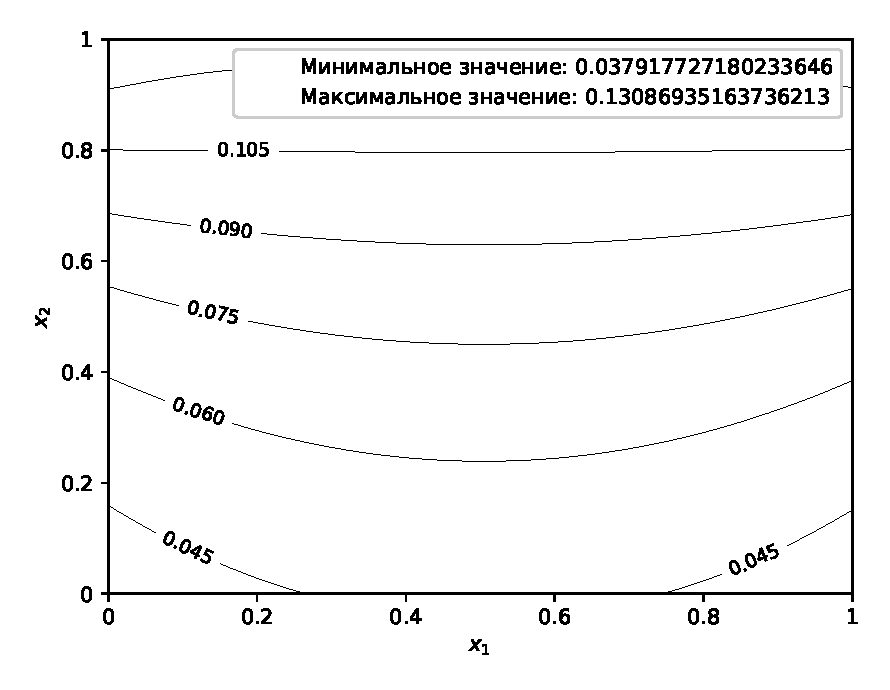
\includegraphics[width=1\linewidth]{boundary/theta_iso_auto} \\ а) $\theta$
    \end{minipage}
    \hfill
    \begin{minipage}[b][][b]{0.49\linewidth}
        \centering
        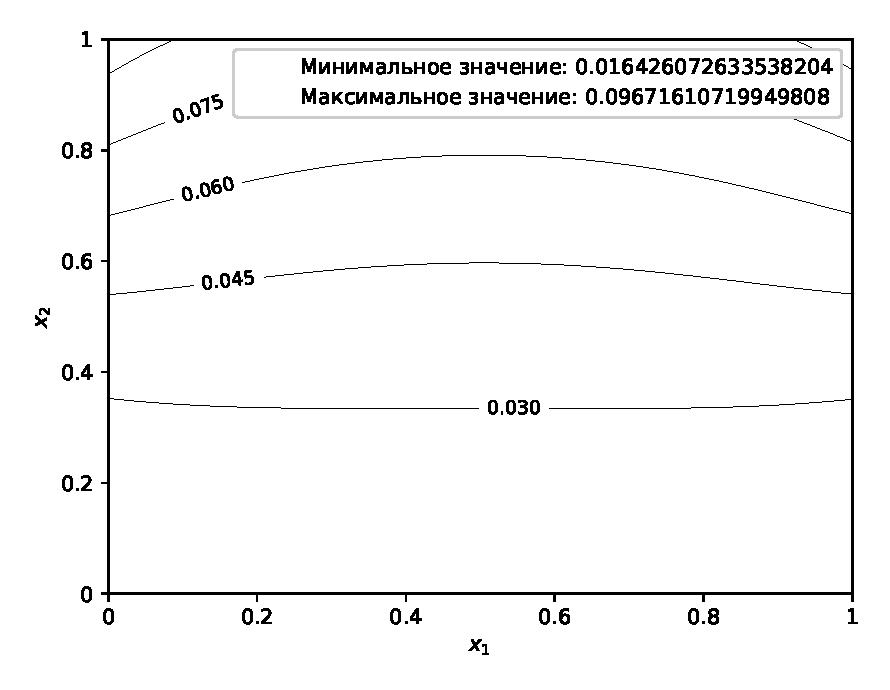
\includegraphics[width=1\linewidth]{boundary/phi_iso_auto} \\ б) $\varphi$
    \end{minipage}
    \caption{Решение граничной задачи}
    \label{fig:4_1:boundary}
\end{figure}


Код, используемый для получения решения представлен в приложении~\ref{lst:boundary}.
Инструментарий для получения изображений можно найти в репозитории~\cite{mesenev-github}.
\begin{remark}
    Алгоритмы численного решения начально-краевых задач для квазилинейных моделей
    также основаны на продложенном выше методе Ньютона и будут изложены при описании
    алгоритмов решения обратных задач.
\end{remark}










    \section{Алгоритмы решения граничных обратных задач}\label{sec:ch4/sec3}

%dvmg368

\subsection{Градиентный спуск и модификации}
\label{subsec:ch4/sec3/grad}
\textit{Градиентный спуск} - это способ минимизации целевой функции
$f(\mathbf{x}), \mathbf{x} \in X$, путем обновления параметров
в направлении, противоположном градиенту целевой функции
$\nabla f(\mathbf{x})$.
Скорость обучения $\eta$ определяет размер шагов, которые мы делаем,
чтобы достичь (локального) минимума.
Иными словами, мы следуем направлению наклона поверхности,
созданной целевой функцией, вниз до тех пор,
пока не достигнем локального минимума.

Известны различные способы модификации градиентного спуска.
Перечислим некоторые из них.

\textbf{Градиентный спуск с проекцией}

Метод градиентного спуска широко используется для минимизации дифференцируемой
функции $f(\mathbf{x})$, итеративно двигаясь в направлении наибольшего убывания.
Алгоритм осуществляется путем обновления параметров
$\mathbf{x} \in \mathbb{X}$, где $\mathbb{X}$ некоторое гильбертово пространство,
в направлении, противоположном
градиенту функции $\nabla f(\mathbf{x})$ с величиной шага
(скорость обучения) $\eta$.
Этот простой, но мощный алгоритм оптимизации используется во
множестве приложений, таких как машинное обучение, компьютерное
зрение и обработка сигналов.
В некоторых случаях задача оптимизации
имеет дополнительные ограничения, которые могут быть включены в
алгоритм градиентного спуска с использованием проекции.
Представим краткий обзор метода градиентного спуска с проекцией.


Цель алгоритма градиентного спуска - минимизировать функцию
$f(\mathbf{x})$, итеративно обновляя параметры следующим образом:

\[ \mathbf{x}_{k+1} = x_k - \eta \nabla f(\mathbf{x}_k), \]
где $\mathbf{x}_k$ - вектор параметров на итерации $k$,
$\eta$ - величина шага, и $\nabla f(\mathbf{x}_k)$ - градиент
функции на итерации $k$.
Когда задача оптимизации включает ограничения, алгоритм
градиентного спуска должен быть изменен, чтобы учесть эти ограничения.
Один из распространенных подходов состоит в использовании проекции
на множество ограничений.


Пусть $\mathcal{C}$ - множество ограничений.
Алгоритм градиентного спуска с проекцией
можно описать следующим образом:
\[ x_{k+1} = \mathcal{P}_{\mathcal{C}}(x_k - \eta \nabla f(x_k)), \]
где $\mathcal{P}_{\mathcal{C}}(\cdot)$ - оператор проекции
на множество ограничений $\mathcal{C}$.
Проекция обеспечивает сохранение обновленного
вектора параметров $\mathbf{x}_{k+1}$ в пределах множества
ограничений, таким образом, удовлетворяя ограничения задачи.

\textbf{Оператор проекции}
Оператор проекции $\mathcal{P}_{\mathcal{C}}(\cdot)$
проецирует заданную точку на множество ограничений $\mathcal{C}$.
Проекция точки $\mathbf{y}$ на множество $\mathcal{C}$ определяется как:
\[
    \mathcal{P}_{\mathcal{C}}(y) =
    \arg \min_{x \in \mathcal{C}} \|y - x\|^2,
\]
где $\|\cdot\|$ обозначает евклидову норму.
Оператор проекции находит точку в множестве ограничений
$\mathcal{C}$, которая ближе всего к заданной точке $\mathbf{y}$.

\textbf{Примеры множеств ограничений}

Множество ограничений может иметь различные формы
в зависимости от задачи оптимизации.
Некоторые распространенные множества ограничений включают:
\begin{itemize}
    \item \textbf{Ограничения-коробки:} Множество ограничений представляет
    собой коробку, определенную как
    $\mathcal{C} = \{\mathbf{x} \in \mathbb{R}^n , | , a_i
    \leq x_i \leq b_i, , i=1,\dots,n\}$.
    В этом случае оператор проекции можно вычислить поэлементно:
    \[
        (\mathcal{P}_{\mathcal{C}}(y))_i =
        \min(\max(y_i, a_i), b_i), \quad i=1,\dots,n.
    \]

    \item \textbf{Ограничения-шары:} Множество ограничений представляет
    собой закрытый шар с радиусом $r$ и центром $\mathbf{c}$,
    определенный как $\mathcal{C} = \{\mathbf{x} \in \mathbb{R}^n , | ,
    \|\mathbf{x} - \mathbf{c}\| \leq r\}$.
    Оператор проекции для этого множества ограничений:
    \[
        \mathcal{P}_{\mathcal{C}}(y) = c
        + \min\left(1, \frac{r}{\|y-c\|}\right)(y-c).
    \]
    \item \textbf{Ограничения-симплексы:} Множество ограничений
    представляет собой симплекс, определенный как
    $\mathcal{C} = \{\mathbf{x} \in \mathbb{R}^n ,
    | , \mathbf{x} \geq \mathbf{0}, , \sum_{i=1}^n x_i = 1\}$.
    Оператор проекции для этого множества ограничений включает
    более сложный алгоритм, такой как тот,
    который представлен, например~\cite{Duchi2011}.
\end{itemize}

\subsection{Алгоритм нахождения квазирешения обратной задачи}
\label{subsec:ch4/sec3/boundary}

Задача нахождения квазирешения обратной
задачи (см.~\ref{subsec:ch2/sec1/subsec1})
\begin{equation}
    \label{eq:4_3:initial}
    \begin{aligned}
        - a \Delta \theta + b \kappa_a(\theta ^ 3 | \theta | - \varphi) = 0,  \\
        - \alpha \Delta \varphi + \kappa_a (\varphi - \theta ^3 | \theta |) = 0.
    \end{aligned}
\end{equation}
\begin{equation}
    \label{eq:4_3:initial-boundary}
    \begin{aligned}
        \Gamma &: \; a \partial_n \theta + \beta (\theta - \theta _b) = 0, \\
        \Gamma_0 \cup \Gamma_2 &: \; \alpha \partial_n \varphi
        + \gamma(\varphi - \theta_b ^4 ) = 0, \\
        \Gamma_1 &: \; \alpha \partial_n \varphi + u(\varphi - \theta_b ^4 ) = 0. \\
    \end{aligned}
\end{equation}
где предполагается, что
\begin{equation}
    \label{eq:4_3:control_bounds}
    0 < u_1 \leq u \leq u_2,
\end{equation}
заключается в минимизации функционала~\eqref{eq:2_1:quality}
\begin{equation}
    \label{eq:4_3:quality}
    J(\theta) = \frac{1}{2} \int_{\Gamma_2} (\theta - \theta_0)^2 d\Gamma
\end{equation}
на решениях начально-краевой задачи~\eqref{eq:4_3:initial}--\eqref{eq:4_3:control_bounds},
с учетом дополнительного условия на участке границы $\Gamma_2$:
\begin{equation}
    \label{eq:4_3:theta_gamma}
    \theta|_{\Gamma_2}=\theta_0.
\end{equation}

Пусть функционал $J(\theta)$ удовлетворяет условиям,
указанным в \autoref{subsec:ch2/sec1/subsec3}.
Для удобства введём переобозначение
$\hat{J}(u)\coloneqq J(\theta(u)), \hat{J}:L^2(\Gamma_1) \to \mathbb{R}$.
Здесь $\theta(u)$ -- температурное поле
задачи~\eqref{eq:2_1:initial}--\eqref{eq:2_1:initial-boundary}
отвечающее управлению $u \in L^2(\Gamma_1)$.

Согласно формуле~\eqref{eq:2_1:therorem_2_eq3}
градиент функционала $\hat{J}(u)$~\cite{Grenkin2016a} имеет вид
\[
    \hat{J}'(u)= (\varphi(u) -\theta_b^4)p_2,
\]
где $\varphi(u)$ есть интенсивность излучения,
$p_2$ -- соответствующая переменная сопряжённой системы.

Предлагаемый алгоритм решения выглядит следующим образом:

%\begin{algorithm}[H]
%    \caption{Алгоритм градиентного спуска с проекцией}
%    \begin{algorithmic}[1]
%        \State Выбираем значение градиентного шага $\lambda$,
%        \State Выбираем количество итераций $N$,
%        \State Выбираем произвольное $u_0 \in U_{ad}$,
%        \For{$k \gets 0,1,2,...,N$}
%            :
%            \State Для полученного $u_k$ расчитываем состояние $y_k = \{\theta_k, \varphi_k\}$ из  (\ref{weak_operational}).
%            \State Расчитываем значение функционала качества $J(\theta_k)$ из (\ref{quality}).
%            \State Расчитываем сопряжённое состояние $p_k=\{p_{1k},p_{2k}\}$ из уравнений \eqref{eq:2_1:therorem_2_eq1}--\eqref{eq:2_1:therorem_2_eq2}, где $ \hat{\theta} := \theta_k, \hat{u}=u_k$.
%            \State Пересчитываем управление $u_{k+1} = P_{ad}\left[ u_k - \lambda (\varphi_k - \theta_b^4)p_{2k} \right]$.
%        \EndFor
%    \end{algorithmic}
%\end{algorithm}

\textbf{Алгоритм градиентного спуска с проекцией}

1.\ Выбор значения шага градиента $\lambda$.

2.\ Выбор числа итераций $N$.

3.\ Выбор начального приближения для управления $u_0 \in U_{ad}$.

4.\ для $k \leftarrow 0,1,2, \ldots, N$ выполнить:

\hspace{1cm} a.\ Для заданного $u_{k}$, вычислить состояние $y_k = \{\theta_k, \varphi_k\}$
системы~\eqref{eq:2_1:weakOperational}.

\hspace{1cm} b.\ Вычислить значение функционала качества
$J(\theta_k)$ из уравнения~\eqref{eq:2_1:quality}.

\hspace{1cm} c.\ Расчитать сопряжённое состояние $p_k=\{p_{1k},p_{2k}\}$ из
уравнений \eqref{eq:2_1:therorem_2_eq1}--\eqref{eq:2_1:therorem_2_eq2},
где $ \hat{\theta} := \theta_k, \hat{u}=u_k$.

\hspace{1cm} d.\  Пересчитать управление
$u_{k+1} = P_{ad}\left[ u_k - \lambda (\varphi_k - \theta_b^4)p_{2k} \right]$.


Значение параметра $\lambda$ выбирается согласованным со значением
градиента $J^{\prime}\left(u_{k}\right)=$ $=\left(\varphi_{k}-\theta_{b}^{4}\right) p_{2k}$
таким образом, чтобы значение $\lambda\left(\varphi_{k}-\theta_{b}^{4}\right) p_{2k}$
определяло значимую поправку для $u_{k}$.
В экспериментах, приведённых ниже, значение параметра $\lambda=20$.

Количество итераций $N$ выбирается достаточным для выполнения условия
$J\left(\theta_{N-1}\right)-J\left(\theta_{N}\right)<10^{-15}$.
Эксперименты показывают хорошее восстановление функции $u$ при $N>10^{5}$.

Оператор проекции $P_{ad} : U \to U_{ad}$ определён следующим образом
\[
    P_{ad}[v] =
    \begin{cases}
        u_1, & \text{если } v \le u_1 \\
        v, & \text{если } u_1 < v < u_2 \\
        u_2, & \text{если } v \ge u_2.
    \end{cases}
\]


\textit{Примеры численного моделирования для двумерного случая.}

Положим $\Omega = \{(x,y), 0 \leq x,y \leq 1\}$, $l = 1$ см.
Граница $\partial\Omega$ состоит из участков:
\[
    \begin{aligned}
        \Gamma_0 & = \{x=\{0,1\}, y \in [0,1]\} \\
        \Gamma_1 & = \{x\in [0,1], y=0\}
        - \text{участок с неизвестными отражающими свойствами}, \\
        \Gamma_2 & = \{x \in [0,1], y=1\} - \text{участок наблюдения}.
    \end{aligned}
\]

Будем также далее считать, что $a = 0.006[\text{см}^2/\text{c}]$,
$b=0.025[\text{см}/\text{с}]$, $\beta = 0.00005[\text{см}/\text{с}]$,
$\kappa=1[\text{см}^{-1}]$, $\kappa_s = 0$, $A = 0$, $\gamma = 0.3$.
Указанные параметры соответствуют стеклу~\cite{Grenkin2016a}.
Температуру на границе $\Omega$ положим равной $\theta_b = (x^2+y^2)/3$.

При указанных параметрах для первого эксперимента выберем следующее тестовое
значение функции $u$ (рис.~\ref{fig:4_3:control}а):
\begin{equation}
    \label{eq:4_3:equation}
    u(x)=
    \begin{cases}
        0.01, & \text{если } x \le 0.5, \\
        0.5, & \text{если } x > 0.5,
    \end{cases}
\end{equation}
и для второго эксперимента (рис.~\ref{fig:4_3:control}б):
\begin{equation}
    \label{eq:4_3:test_function_1}
    u(x)=0.49x+0.01.
\end{equation}

Вычислим решение прямой
задачи~\eqref{eq:2_1:initial}--\eqref{eq:2_1:initial-boundary}
для этих случаев.
Полученное температурное поле на участке наблюдения
$\Gamma_2$ выберем в качестве $\theta_0$.
Далее, применяя предложенный алгоритм находим квазирешение обратной
задачи~\eqref{eq:2_1:initial}--\eqref{eq:2_1:theta_gamma}.
Эффективность алгоритма, а также значение $u_0$ в первом и
втором случаях иллюстрируются на рисунке~\ref{fig:4_3:control}.
На рисунке~\ref{fig:4_3:cost} показана динамика функционала качества по итерациям.
\begin{figure}[h!t]
    \begin{minipage}[b][][b]{0.49\linewidth}
        \centering
        \includegraphics[width=1\linewidth]{dvmg368/3} \\ а) Первый эксперимент
    \end{minipage}
    \hfill
    \begin{minipage}[b][][b]{0.49\linewidth}
        \centering
        \includegraphics[width=1\linewidth]{dvmg368/4} \\ б) Второй эксперимент
    \end{minipage}
    \caption{Значение функционала качества}
    \label{fig:4_3:cost}
\end{figure}

\begin{remark}
    В предложенных примерах потребовалось
    $2 \cdot 10^6$ итераций для нахождения квазирешения $u$.
    В то же время температурное поле на участке наблюдения
    $\Gamma_2$ становится близким к $\theta_0$ уже на $10^2$ итерации.
    Также наблюдается существенное падение скорости уменьшения функционала
    качества с каждой итерацией после того, как среднее значение найденной
    функции контроля становится близко к тестовой функции.
\end{remark}

\begin{figure}[h!t]
    \begin{minipage}[b][][b]{0.49\linewidth}
        \centering
        \includegraphics[width=1\linewidth]{dvmg368/1} \\ а) Первый эксперимент
    \end{minipage}
    \hfill
    \begin{minipage}[b][][b]{0.49\linewidth}
        \centering
        \includegraphics[width=1\linewidth]{dvmg368/2} \\ б) Второй эксперимент
    \end{minipage}
    \caption{Тестовая функция $u$, начальная $u_0$, найденная функция $u_{end}.$}
    \label{fig:4_3:control}
\end{figure}

\subsection{Алгоритм решения задачи оптимального управления для квазистационарной модели}
\label{subsec:ch4/sec3/quasistationary}
%paper03
Задача оптимального управления, поставленная в разделе~\ref{sec:ch2/sec3}
для стационарной модели имеет вид:
\begin{equation*}
    J_{\lambda}(\theta, u)=\frac{1}{2} \int_{0}^{T}
    \int_{\Gamma}\left(\theta-\theta_{b}\right)^{2} d \Gamma d t+\frac{\lambda}{2}
    \int_{0}^{T} \int_{\Gamma} u^{2} d \Gamma d t \rightarrow \inf
\end{equation*}
на решениях задачи
\begin{equation}
    \label{eq:4_3:1}
    \begin{split}
        & \frac{\partial \theta}{\partial t} - a \Delta \theta
        + b \kappa_{a} \left(|\theta| \theta^{3}-\varphi\right) = 0,\\
        & - \alpha \Delta \varphi
        + \kappa_{a} \left(\varphi-|\theta| \theta^{3}\right) = 0,
        \quad x \in \Omega, \quad 0 < t < T;
    \end{split}
\end{equation}
\begin{align}
    a \left(\partial_{n} \theta+\theta\right)=r,
    & \quad \alpha\left(\partial_{n} \varphi
    + \varphi\right) = u \text { на } \Gamma;  \label{eq:4_3:2}\\
    & \left.\theta\right|_{t=0} = \theta_{0}. \label{eq:4_3:3}
\end{align}
Напомним, что эта задача аппрокисимрует задачу с данными типа Коши для температуры.



Приведем алгоритм решения задачи управления.
Пусть
\[
    \widetilde{J}_{\lambda}(u)=J_{\lambda}(\theta(u), u),
\]
где $\theta(u)$ — компонента решения
задачи~\eqref{eq:2_3:1}--\eqref{eq:2_3:2},
соответствующая управлению $u \in U$.
Согласно~\eqref{eq:2_3:15} градиент функционала
$\widetilde{J}_{\lambda}(u)$ определяется
следующим образом: $\widetilde{J}_{\lambda}^{\prime}(u) = \lambda u-p_{2}$.
Здесь $p_{2}$ — соответствующая компонента сопряженного
состояния системы~\eqref{eq:2_3:15}
        \begin{gather*}
            -p_{1}^{\prime}+a A p_{1}+4|\widehat{\theta}|^{3} \kappa_{a}\left(b p_{1}
            -p_{2}\right)=B\left(\theta_{b}-\widehat{\theta}\right), \\
            p_{1}(T)=0,\; \alpha A p_{2}+\kappa_{a}\left(p_{2}-b p_{1}\right)=0,
        \end{gather*}
где $\widehat{\theta}\coloneqq\theta(u)$.
Предлагаемый алгоритм для решения задачи оптимального управления
состоит из следующих шагов:

\textbf{Алгоритм градиентного спуска}

1.\ Выбор значения шага градиента $\varepsilon$,

2.\ Выбор числа итераций $N$,

3.\ Выбор начального приближения для управления $u_{0} \in U$,

4.\ для $k \leftarrow 0,1,2, \ldots, N$ выполнить:

\hspace{1cm} a.\ Для заданного $u_{k}$, вычислить состояние
$y_{k}=\left\{\theta_{k}, \varphi_{k}\right\}$, решение
задачи~\eqref{eq:2_3:1}--\eqref{eq:2_3:3}.

\hspace{1cm} b.\ Вычислить значение функционала качества
$J_{\lambda}\left(\theta_{k}, u_{k}\right)$.

\hspace{1cm} c.\ Из уравнений~\eqref{eq:2_3:15}, вычислить сопряженное
состояние $p_{k}=\left\{p_{1 k}, p_{2 k}\right\}$,
где $\widehat{\theta} \coloneqq \theta_{k}, \widehat{u} \coloneqq u_{k}$.

\hspace{1cm} d.\ Пересчитать управление
$u_{k+1}=u_{k}-\varepsilon\left(\lambda u_{k}-p_{2}\right)$

Параметр $\varepsilon$ выбирается эмпирически таким образом, чтобы
значение $\varepsilon\left(\lambda u_{k}-p_{2}\right)$ являлось
существенной корректировкой для $u_{k+1}$.
Число итераций $N$ выбирается достаточным для
удовлетворения условия $J_{\lambda}\left(\theta_{k}, u_{k}\right)
-J_{\lambda}\left(\theta_{k+1}, u_{k+1}\right)<\delta$, где $\delta>0$
определяет точность вычислений.

Рассмотренный ниже пример иллюстрирует работу предложенного
алгоритма для малых, что важно, значений параметра регуляризации
$\lambda \leq 10^{-12}$.


Заметим, что для численного решения прямой задачи с заданным управлением
был использован метод простой итерации для линеаризации задачи и ее решения
с помощью метода конечных элементов.
Для численного моделирования мы использовали солвер FEniCS~\cite{fenics, dolfin}.
Сравним работу предложенного
алгоритма с результатами статьи~\cite{Chebotarev2019Problem}.
Задача рассматривается в области $\Omega \times(-L, L)$,
где $\Omega=$ $\left\{x=\left(x_{1}, x_{2}\right): 0<x_{1,2}<d\right\}$
и при большом $L$ сводится к двумерной задаче для вычислительной
области $\Omega$.

Для задачи были выбраны следующие значения параметров:
$d=1(\text{м}), a=0.9210^{-4}(\text{м}^{2} / \text{с}),
b=0.19(\text{м} / \text{с})$, $\alpha=0.0333(\text{м}),
\kappa_{a}=1\left(\text{м}^{-1}\right)$.
Параметры соответствуют воздуху при нормальном атмосферном давлении
и температуре $400^{\circ} \text{C}$.
Функции $\theta_{b}, q_{b}$ для граничного условия~\eqref{eq:2_3:5}
задаются следующим образом: $\theta_{b}=\left.\widehat{\theta}\right|_{\Gamma},
q_{b}=\left.\partial_{n} \widehat{\theta}\right|_{\Gamma}$,
где $\widehat{\theta}=$ $\left(x_{1}-0.5\right)^{2}-0.5 x_{2}+0.75$.

Приближенное решение задачи~\eqref{eq:2_3:16},\eqref{eq:2_3:17}
с данными Коши, представленными в~\cite{Chebotarev2019Problem}
(рисунок~\ref{fig:4_3:1}а), было получено путем решения параболической задачи
четвертого порядка для температуры.
Решение стабилизировалось через 120 секунд, но
вычисления на каждом временном шаге были
довольно затратными~\cite{Chebotarev2019Problem}.
\begin{figure}[h!t]
    \begin{minipage}[b][][b]{0.49\linewidth}
        \centering
        \includegraphics[width=1\linewidth]{paper03/1} \\ а) Поле температуры,
        полученное в статье~\cite{Chebotarev2019Problem}
    \end{minipage}
    \hfill
    \begin{minipage}[b][][b]{0.49\linewidth}
        \centering
        \includegraphics[width=1\linewidth]{paper03/2} \\
        б) Поле температуры, полученное предложенным алгоритмом
    \end{minipage}
    \caption{сравнение полученных температурных полей}
    \label{fig:4_3:1}
\end{figure}
На рисунке~\ref{fig:4_3:1}б показано стационарное поле температуры,
полученное с помощью метода, предложенного в данном параграфе.

Представленный пример иллюстрирует, что предложенный
алгоритм успешно находит численное решение
задачи~\eqref{eq:2_3:16},\eqref{eq:2_3:17} с граничными
условиями типа Коши.

%6_Chebotarev

%6_cheb
\label{subsec:ch4/sec3/quasilinear}
Перенос тепла и излучения будет рассматриваться в среде,
состоящей из четырех частей, которые интерпретируются как кровь,
стенки вены, около-венозная ткань и оптическое волокно.
Вычислительная область в цилиндрической системе координат в случае
угловой симметрии схематически изображена на рисунке~\ref{fig:4_3:3}
(линейные размеры указаны в миллиметрах).

\begin{figure}[h!t]
    \centerfloat{\includegraphics[scale=0.35]{6_cheb/1}}
    \caption{Область вычисления}
    \label{fig:4_3:3}
\end{figure}
%\ref{fig:4_3:3}
Для нахождения решения начально-краевой
задачи~\eqref{eq:1_6:1}--\eqref{eq:1_6:3}
мы дискретизируем временной интервал
$(0, T), \quad 0=t_{0}<t_{1}<t_{2}<\ldots<t_{N}=T$.
Для каждого момента времени $t=t_{l}=l \Delta t$, $l=1,2, \ldots, N$,
используется итерационный алгоритм для нахождения решения соответствующей
краевой задачи. $n$-й шаг итерационной процедуры $(n=1,2, \ldots, M)$
записывается следующим образом:
\begin{gather}
    -\operatorname{div}\left(\alpha \nabla \varphi_{n}\right)
    +\beta\left(\varphi_{n}-\theta_{n-1}^{3}
    \left|\theta_{n-1}\right|\right)=g, \label{eq:3_1:22}\\
    \sigma \partial \theta_{n} / \partial t
    -\operatorname{div}\left(k\left(\theta_{n-1}\right)
    \nabla \theta_{n}\right)
    -b\left(\theta_{n-1}^{3}\left|\theta_{n}\right|
    -\varphi_{n}\right)=f, \quad x \in \Omega, \label{eq:3_1:23}\\
    k\left(\theta_{n-1}\right) \partial_{n} \theta_{n}
    +\left.p\left(\theta_{n}-\theta_{b}\right)\right|_{\Gamma}=0,
    \quad \alpha \partial_{n} \varphi_{n}+\left.\gamma
    \left(\varphi_{n}-\theta_{b}^{4}\right)\right|_{\Gamma}=0,\label{eq:3_1:24}
\end{gather}
где производная по времени в~\eqref{eq:3_1:23}
аппроксимируется следующим образом
\[
    \frac{\partial \theta_{n}}{\partial t} \simeq
    \frac{
        \left.\theta_{n}\right|_{t=t_{l}}
        -\left.\theta_{M}\right|_{t=t_{l-1}}
    }{\Delta t},
\]
и функции $\theta_{n}, \theta_{n-1}, \varphi_{n}$
в~\eqref{eq:3_1:22}--\eqref{eq:3_1:24} являются приближениями решения,
соответствующими моменту времени $t=t_{l}$.
Подстрочный индекс функций
$\theta_{n}, \theta_{n-1}$ и $\varphi_{n}$ означает номер итерации.
Для инициализации итерационной процедуры задаем начальное приближение
температуры для каждого момента времени:
\begin{equation}
    \label{eq:3_1:25}
    \left.\theta_{0}\right|_{t=t_{l}}=
    \left.\theta_{M}\right|_{t=t_{l-1}},
    \quad l=1,2, \ldots, N, \left.\quad
    \theta_{M}\right|_{t=t_{0}}=\theta_{i n}.
\end{equation}

В уравнениях~\eqref{eq:3_1:22},\eqref{eq:3_1:23}
$g=P_{\varphi} \chi / \mathcal{M}{\varphi},
f=P{\theta} \chi / \mathcal{M}{\theta}$,
где $P{\varphi}$ - мощность источника, расходуемая на излучение,
$P_{\theta}$ описывает мощность источника, расходуемую на нагрев
кончика волокна, $\chi$ - характеристическая функция части среды,
в которой расположен кончик волокна, деленная на объем кончика волокна,
$\mathcal{M}{\varphi}$ и $\mathcal{M}{\theta}$ - нормализующие коэффициенты
для получения средней интенсивности излучения
и абсолютной температуры из $\varphi$ и $\theta$.

Для реализации каждого шага итерационного
алгоритма~\eqref{eq:3_1:22}--\eqref{eq:3_1:25}
использовался метод конечных элементов с использованием
программного пакета FreeFEM++\cite{Hecht2012}.
Оптические и термофизические параметры среды
взяты из~\cite{Opticalthermal_vanRuijven2014}.
Параметры $\theta_{b}$ и $\theta_{i n}$ соответствуют
температуре $37^{\circ} \text{C}$, а коэффициент $\gamma$ равен 1.
Во всех расчетах начальное положение кончика оптического волокна
соответствует $(r, z)=(0,5)$, и его скорость отката составляет
$2 \text{~мм} / \text{с}$.
Следуя~\cite{van2014optical, Some_Poluektova2014},
мы моделируем теплоперенос потоком пузырьков,
образующихся на горячем кончике волокна, через коэффициент теплопроводности,
зависящий от температуры, как следующим образом: когда температура
в определенной точке достигает $95^{\circ}\text{~C}$ и выше,
коэффициент теплопроводности увеличивается в 200 раз.

Эффективность лазерной абляции можно оценить по поведению
температурных профилей в различных точках вычислительной области.
Основные параметры процедуры лазерной абляции -- мощность лазера,
длина волны излучения, скорость отката оптического волокна и
соотношение между мощностями лазера, затрачиваемыми на
излучение и нагрев кончика волокна.

Отметим,что решение задачи~\eqref{eq:1_6:1}--\eqref{eq:1_6:3} зависит от длины
волны неявным образом, через параметры $\alpha$ и $\beta$,
описывающие свойства излучения среды (смотрите таблицы значений коэффициента
поглощения и коэффициента уменьшения рассеяния, определяющие параметры
$\alpha$ и $\beta$~\cite{Opticalthermal_vanRuijven2014, Some_Poluektova2014}.
Как правило, лазерная абляция осуществляется излучением с длиной волны
от \(810\) до $1950$~нм.
Достаточно широко используемые диапазоны скорости отката волокна и мощности
лазерного излучения составляют $1-3\text{~мм}/\text{с}$
и $5-15$~Вт
соответственно~\cite{
    Mathematical_Mordon2006,
    Opticalthermal_vanRuijven2014,
    Some_Poluektova2014}.


\begin{figure}[h!t]
    \centerfloat{\includegraphics[scale=0.33]{6_cheb/2}}
    \caption{Поведение температуры в точке $(1.5,10)$
        при мощности лазера $10\text{~Вт}$ и следующих длинах волн:
        $810\text{~нм}$ (черный), $1064\text{~нм}$ (красный),
        $1470\text{~нм}$ (зеленый) и $1950\text{~нм}$ (синий).}
    \label{fig:4_3:4}
\end{figure}

Рисунок~\ref{fig:4_3:4} показывает поведение температурных профилей в точке $(1.5,10)$ для
излучения с различными длинами волн: $810 \text{~нм}, 1064 \text{~нм},
1470 \text{~нм}$ и $1950 \text{~нм}$.
Мощность источника устанавливается как $\left(P_{\varphi}, P_{\theta}\right)
=(7 \text{~Вт}, 3 \text{~Вт})$ во всех случаях.
Как видно из рисунка~\ref{fig:4_3:4}, изменение длины волны излучения оказывает
значительное влияние на поведение температурного профиля.
Тем не менее, возможно обеспечить достаточно близкую продолжительность
кипения (когда температура выше $95^{\circ} \text{C}$) для температурных
профилей, соответствующих разным длинам волн, изменив мощность
лазера $P=P_{\varphi}+P_{\theta}$, сохраняя соотношение
$P_{\varphi} / P_{\theta}$ равным $7 / 3$ (рисунок~\ref{fig:4_3:4}).
Отметим, что рассчитанная температура в точках перивенозной ткани,
$(2.5,10)$ и $(3.5,10)$, довольно безопасна (рисунок~\ref{fig:4_3:5}).

Как видно из проведенных экспериментов, использование компьютерного
моделирования является перспективным способом определения оптимальных
параметров излучения, обеспечивающих эффективную и безопасную процедуру ЭВЛА.

На рисунке~\ref{fig:4_3:4} показаны температурные профили
в точке $(1.5, 10)$ для мощности лазера
$10 \text{~Вт}$ и для разных длин волн: $810 \text{~нм}$ (черный),
$1064 \text{~нм}$ (красный), $1470 \text{~нм}$
(зеленый) и $1950 \text{~нм}$ (синий).

\begin{figure}[h!t]
    \centerfloat{\includegraphics[scale=0.33]{6_cheb/3}}
    \caption{Поведение температуры в точке $(1.5,10)$
        для следующих длин волн и мощностей лазера:
        $810 \text{~нм}, P=10 \text{~Вт}$ (черный);
        $1064 \text{~нм}, P=11 \text{~W}$ (красный);
        $1470 \text{~нм}, P=7,5 \text{~W}$ (зеленый);
        $1950 \text{~нм}, P=6 \text{~W}$ (синий).}
    \label{fig:4_3:5}
\end{figure}
На рисунке~\ref{fig:4_3:5} показаны температурные профили в точке $(1.5,10)$ для разных
длин волн и мощности лазера: $810 \text{~нм}$, $P=10 \text{~Вт}$
(черный); $1064 \text{~нм}, P=11 \text{~Вт}$ (красный);
$1470 \text{~нм}, P=7.5 \text{~Вт}$ (зеленый);
$1950 \text{~нм}, P=6 \text{~Вт}$ (синий).


\begin{figure}[h!t]
    \centerfloat{\includegraphics[scale=0.33]{6_cheb/4}}
    \caption{Поведение температуры в точках $(1.5,10)$ (твердое тело),
        $(2.5,10)$ ( пунктирной линией) и $(3,5,10)$ (пунктирной линией).
        Длина волны равна $810 \text{~нм},\left(P_{\varphi},
        P_{\theta}\right)=(7 \text{~W}, 3 \text{~W})$.}
    \label{fig:4_3:6}
\end{figure}
На рисунке~\ref{fig:4_3:6} показаны температурные профили в точках $(1.5,10)$ (сплошной),
$(2.5,10)$ (пунктирный) и $(3.5,10)$ (точка-тире).
Длина волны составляет $810 \text{~нм},\left(P_{\varphi},
P_{\theta}\right)=(7 \text{~Вт}, 3 \text{~Вт})$


%Chebotarev_2 nd, Chebotarev_Park_Mesenev_Kovtanyuk_21

\subsection{Метод штрафов для задачи с фазовыми ограничениями}
\label{subsec:ch4/sec3/subsec5}
Квазилинейная модель радиационного и диффузионного теплообмена в ограниченной области
$\Omega \subset \mathbb{R}^{3}$ с границей $\Gamma=\partial \Omega$
в разделе~\ref{sec:ch3:sec2} представлена в виде начально-краевой задачи
следующим образом:
\begin{equation*}
\begin{aligned}
& \sigma \partial \theta / \partial t-\operatorname{div}(k(\theta) \nabla \theta)-\beta \varphi=u_{1} \chi, \\
& -\operatorname{div}(\alpha \nabla \varphi)+\beta \varphi=u_{2} \chi, \quad x \in \Omega, \quad t \in(0, T), \\
& \theta=\left.0\right|_{\Gamma}, \quad \alpha \partial_{n}
    \varphi+\left.2^{-1} \varphi\right|_{\Gamma}=0,\left.\quad \theta\right|_{t=0}=\theta_{0} .
\end{aligned}
\end{equation*}
Требуется найти неизвестные интенсивности $u_1,\, u_2$ и соответствующие поля $\theta, \, \varphi$
по условию
\[
    J(\theta)=\int_{0}^{T}
    \int_{G_{1}}\left(\theta-\theta_{d}\right)^{2} d x d t \rightarrow \inf,
\]
при ограничениях
\[
    u_{1,2} \geq 0, \quad u_{1}+u_{2} \leq P,\left.\quad \theta\right|_{G_{2}} \leq \theta_{*}.
\]

В разделе~\ref{subsec:ch3/sec2/penalty} показано, что задачу с ограничениями
на температуру в области $G_2$ можно
аппрокисимировать задачей со штрафом $P_\varepsilon$.


Рассмотрим итерационный алгоритм решения задачи оптимального управления
$\left(P_{\varepsilon}\right)$ для случая, когда параметры управления
$u_{1}$ и $u_{2}$ не зависят от времени.
На каждой итерации алгоритма
решается линейно-квадратичная задача оптимального управления,
в которой требуется найти минимум функционала:

\begin{equation}
    \label{eq:3_2:9}
    \begin{aligned}
        &\widehat{J}_{\varepsilon}(\theta)=\int_{0}^{T}
        \int_{G_{1}}\left(\theta-\theta_{d}\right)^{2} d x d t \\
        &+\frac{1}{\varepsilon} \int_{0}^{T}
        \int_{G_{*}}\left(\theta-\theta_{*}\right)^{2} d x d t
        \rightarrow \inf , \quad u \in U_{a d}
    \end{aligned}
\end{equation}

с соответствующими ограничениями
\begin{equation}
    \label{eq:3_2:10}
    \begin{aligned}
        &\sigma \partial \theta / \partial t-\operatorname{div}(k(\widehat{\theta})
        \nabla \theta)=u, \quad x \in \Omega, \quad 0<t<T, \\
        &\left.\theta\right|_{\Gamma}=0, \quad \theta(x, 0)=\theta_{0}.
    \end{aligned}
\end{equation}

Здесь,
\[
    \begin{gathered}
        U_{a d}=\left\{u=u_{1} \chi+u_{2} \beta B^{-1} \chi: u_{1,2} \in \mathbb{R},\right. \\
        \left.u_{1,2} \geq 0, u_{1}+u_{2} \leq P\right\}, \\
        G_{*}=\left\{x \in G_{2}: \hat{\theta}(x, t)>\theta_{*}\right\}.
    \end{gathered}
\]

Функция $\widehat{\theta}$ описывает поле температуры,
найденное на предыдущей итерации.

В качестве зависимости коэффициента теплопроводности от температуры используется
гладкая аппроксимация кусочно-постоянной функции, рассмотренной
в~\cite{Opticalthermal_vanRuijven2014, Some_Poluektova2014, Endovenous_Malskat2014},

Как легко видеть, задача~\eqref{eq:3_2:9},\eqref{eq:3_2:10} сводится к
нахождению минимума квадратичной функции параметров $u_{1}$ и $u_{2}$:

\[
    \widehat{J}_{\varepsilon}\left(u_{1} \theta_{1}+u_{2} \theta_{2}+\theta_{3}\right) \rightarrow \inf
\]
на треугольнике  $\left\{u_{1}, u_{2} \in \mathbb{R}:
u_{1,2} \geq 0, u_{1}+u_{2} \leq P\right\}$.
Функции $\theta_{1}, \theta_{2}$ и $\theta_{3}$
вычисляются заранее как решения следующих линейных
начально-краевых задач для $x \in \Omega, t \in(0, T)$:


\[
    \begin{aligned}
        &\sigma \partial \theta_{1} / \partial t-\operatorname{div}\left(k(\widehat{\theta})
        \nabla \theta_{1}\right)=\chi, &
        \left.\theta_{1}\right|_{\Gamma}=0, \quad \theta_{1}(x, 0)=0, \\
        &\sigma \partial \theta_{2} / \partial t-\operatorname{div}\left(k(\widehat{\theta})
        \nabla \theta_{2}\right)=\beta B^{-1} \chi, &
        \left.\theta_{2}\right|_{\Gamma}=0, \quad \theta_{2}(x, 0)=0, \\
        &\sigma \partial \theta_{3} / \partial t-\operatorname{div}\left(k(\widehat{\theta})
        \nabla \theta_{3}\right)=0, &
        \left.\theta_{3}\right|_{\Gamma}=0, \quad \theta_{3}(x, 0)=\theta_{0}.
    \end{aligned}
\]

При проведении численных экспериментов использовалась область,
аналогичная рассматриваемой в разделе~\ref{subsec:ch4/sec3/quasilinear}
(рисунок~\ref{fig:4_3:3}).
Толщина карбонизированного слоя равна $0,2 \text{~мм}$,
скорость вытягивания волокна $2 \text{~мм}/\text{s}$.
Рассматривалось излучение с длиной волны $1064 \text{~нм}$.
Оптические и теплофизические параметры среды взяты
из~\cite{Opticalthermal_vanRuijven2014, Some_Poluektova2014, Endovenous_Malskat2014}.


Для демонстрации сходимости итерационного алгоритма в качестве
решения прямой начально-краевой задачи для $\left(u_{1}, u_{2}\right)=( 3,7)$
(здесь и далее единицы в ваттах).
Области $G_{1}$ и $G_{2}$ берутся как достаточно малые окрестности
точек $(1.5,10),(3.5,10)$.
Для реализации итерационного алгоритма мы взяли $\varepsilon=0.3$ и $\theta_{*}$,
соответствующие $47^{\circ} \text{C}$.


\begin{figure}[h!t]
    \centerfloat{\includegraphics[scale=0.33]{2_cheb/2}}
    \caption{Температурные профили: желаемая температура (черный),
        1-е (зеленое), 2-е (синее) и 3-е (красное) приближения.}
    \label{fig:4_3:7}
\end{figure}



Аппроксимации решения в точке $(1.5,10)$ показаны на рисунке~\ref{fig:4_3:7}.
Аппроксимации после 1-го, 2-го и 3-го шагов итерационного
алгоритма отмечены зеленым цветом
$\left(u_{1 }, u_{2}\right)=(2.5,4.8)$,
синим  $\left(u_{1}, u_{2}\right)=(3.4,3.5)$
и красным $\left(u_{1}, u_{2}\right)=(4.2,0.9)$ соответственно.
Черная линия показывает желаемую температуру, соответствующую
$\left(u_{1}, u_{2}\right)=(3,7)$.
Максимальное значение температуры в точке $(3.5,10)$ равно $48,8^{\circ}\text{C}$.
Отметим, что при $\left(u_{1}, u_{2}\right)=(3,7)$ максимальное значение
температуры в точке $(3.5,10)$ равно $50,2^{ \circ} \text{C}$.

Данный пример демонстрирует возможность снижения температуры в
околовенозной ткани при сохранении температурного режима внутри вены.

    \section{Алгоритмы решения задач с данными Коши. Примеры.}\label{sec:ch4/sec4}

%VYC0036
\subsection{
    Решение задачи сложного теплообмена
    с граничными условиями типа коши
}\label{subsec:ch4/sec4/subsec1}

Представим итерационный алгоритм решения задачи оптимального управления.
Пусть $\tilde J_\lambda(u)=J_\lambda(\theta(u), u)$, где $\theta(u)$ компонента решения
задачи~\eqref{eq:2_2:eq1},\eqref{eq:2_2:bc2}, соответствующая управлению $u\in U$.

В соответствии с~\eqref{eq:2_2:as} градиент функционала $\tilde J_\lambda(u)$ равен
\[
    \tilde J'_\lambda (u) = \lambda u - p_2.
\]
Здесь $p_2$ -- соответствующая компонента сопряженного
состояния из системы~\eqref{eq:2_2:as}, где $\hat{\theta}\coloneqq\theta(u)$.

%\begin{algorithm}[H]
%    \caption{Алгоритм градиентного спуска}
%    \label{alg:algorithm}
%    \begin{algorithmic}[1]
%        \State Выбираем значение градиентного шага $\varepsilon$,
%        \State Выбираем количество итераций $N$,
%        \State Выбираем начальное приближение для управления $u_0 \in U$,
%        \For{$k \gets 0,1,2,\dots,N$}
%            \State Для данного $u_k$ рассчитываем состояние $y_k = \{\theta_k, \varphi_k\}$ --
%            решение задачи~\eqref{eq:2_2:eq1},\eqref{eq:2_2:bc1}.
%            \State Рассчитываем значение функционала качества $J_\lambda(\theta_k, u_k)$.
%            \State Рассчитываем сопряженное состояние
%$p_k=\{p_{1k},p_{2k}\}$ из уравнений~\eqref{eq:2_2:oc1},
%            где $ \hat{\theta} \coloneqq \theta_k, \hat{u}=u_k$.
%            \State Пересчитываем управление $u_{k+1} = u_k - \varepsilon (\lambda u_k - p_2)$
%        \EndFor
%    \end{algorithmic}
%\end{algorithm}

Значение параметра $\varepsilon$ выбирается эмпирически таким образом, чтобы значение
$\varepsilon (\lambda u_k - p_2)$ являлось существенной поправкой для $u_{k+1}$.
Количество итераций $N$ выбирается достаточным для выполнения условия
$J_\lambda(\theta_k, u_k) - J_\lambda(\theta_{k+1}, u_{k+1}) < \delta$, где $\delta>0$
определяет точность расчетов.

Примеры, рассмотренные ниже, иллюстрируют работоспособность предложенного алгоритма при
малых, что важно, значениях параметра регуляризации $\lambda \leq 10^{-12}$.
В первом примере выполнены тестовые расчеты для куба.
Во втором примере приводится сравнение расчетов по
предложенному алгоритму с результатами работы~\cite{Chebotarev2019Problem}.

Отметим, что для численного решения прямой задачи с заданным управлением использовался
метод простой итерации для линеаризации задачи и ее решения методом конечных элементов.
Решение сопряженной системы, которая является линейной при заданной температуре,
не вызывает трудностей.
Для численного моделирования использовался солвер FEniCS~\cite{fenics, dolfin}.

Исходный код экспериментов можно найти по ссылке~\cite{mesenev-github}.

\textbf{Пример 1.}

Приведем примеры расчетов для куба $\Omega = {(x, y, z), 0 \leq x,y,z \leq l}$.
Будем считать, что $l=1~\text{см}$, $a = 0.006[\text{см}^2/\text{c}]$,
$b=0.025[\text{см}/\text{с}]$, $\kappa_a=1[\text{см}^{-1}]$, $\alpha = 0.(3)[\text{см}]$.
Указанные параметры соответствуют стеклу~\cite{Grenkin2016a}.
Параметр регуляризации $\lambda=10^{-12}.$

Пусть граничные данные $r$ и $u$ в~\eqref{eq:2_2:bc1} имеют вид:
\begin{gather*}
    r = 0.7,\\
    u = \hat u = 0.5.
\end{gather*}
Далее рассчитываем состояние $\theta$ и $\varphi$ как решение
задачи~\eqref{eq:2_2:eq1},\eqref{eq:2_2:bc1} и в качестве $\theta_b$
выбираем граничное значение функции $\theta$ на $\Gamma$.
Значения нормальной производной $\partial_n\theta$ на $\Gamma$
должны соответствовать значениям $q_b=r/a-\theta_b$.
Применяя предложенный алгоритм с начальным приближением $u_0 = 0.1$,
находим приближенное решение $\{\theta_\lambda, \varphi_\lambda, u_\lambda\}$ задачи $CP$.
Для демонстрации того, что алгоритм находит приближенное решение задачи с данными
Коши для температуры, важно сравнить значения $\partial_n\theta_\lambda$ на $\Gamma$ с $q_b.$

На рисунке~\ref{fig:4_4:0}а представлен модуль относительного
отклонения $\partial_n\theta_\lambda$ от $q_b$ на грани куба в плоскости $z=l$,
где $\partial_n\theta_\lambda=\partial\theta_\lambda/\partial z$,
а также динамика функционала качества, определяющего норму
разности $\|\theta_\lambda -\theta_b\|^2_\Gamma$ на рисунке~\ref{fig:4_4:0}б.
На остальных гранях куба значения относительного
отклонения имеют тот же порядок малости.

\begin{figure}[ht]
    \begin{minipage}[b][][b]{0.49\linewidth}
        \centering
        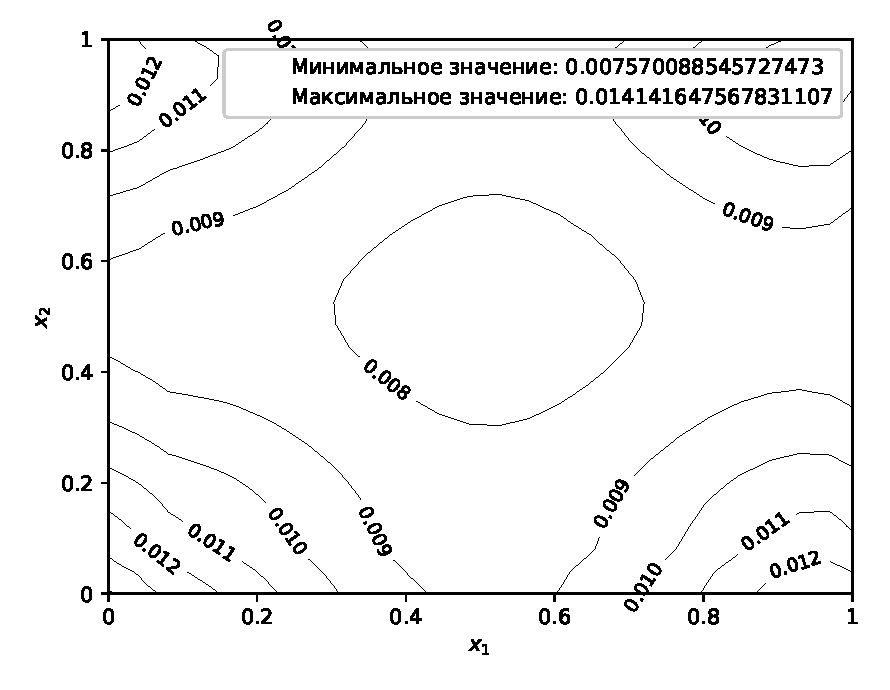
\includegraphics[width=1\linewidth]{jvm-2020/exp1/theta_n_diff_iso}
        \\ а) $|\partial_n\theta_\lambda-q_b|/|q_b|$
    \end{minipage}
    \hfill
    \begin{minipage}[b][][b]{0.49\linewidth}
        \centering
        \includegraphics[width=1\linewidth]{jvm-2020/exp1/quality}
        \\ б) Результаты первого эксперимента
    \end{minipage}
    \caption{Значение функционала качества}
    \label{fig:4_4:0}
\end{figure}

\textbf{Пример 2.}
Сравним работу предложенного алгоритма с результатами статьи~\cite{Chebotarev2019Problem},
где соавтором был один из авторов данной работы.
Задача рассматривается в области $\Omega \times (-L,L)$,
где $\Omega = \{ x = (x_1,x_2) \colon 0 < x_{1,2} < d\}$
и при больших $L$ сводится к двумерной задаче с вычислительной областью $\Omega$.
Выбраны следующие значения параметров задачи:
$d = \mathrm{1(m)}$, $a = 0.92~10^{-4}~\mathrm{(m^2/s)}$, $b= 0.19~\mathrm{(m/s)}$,
$\alpha = 0.0333~\mathrm{(m)}$ и $\kappa_a = 1~\mathrm{(m^{-1})}$.
Параметры соответствуют воздуху при нормальном атмосферном давлении и температуре 400$^\circ$C\@.

Функции $\theta_b$, $q_b$ в краевом условии~\eqref{eq:2_2:bc2} заданы следующим образом:
$\theta_b = \widehat{\theta}|_{\Gamma}$, $q_b = \partial_n \widehat{\theta}|_{\Gamma}$, где
$\widehat{\theta} = (x_1-0.5)^2 - 0.5x_2+0.75$.

Приближенное решение задачи с данными Коши, представленное в~\cite{Chebotarev2019Problem}
получено путем решения эллиптической задачи четвертого
порядка для температуры методом установления по времени.
Использовались $H^2$ конформные конечные элементы Богнера-Фокса-Шмитта и
солвер FeliCs, разработанный в техническом университете Мюнхена.
Решение стабилизировалось через 120 секунд, но вычисления на каждом временном
шаге потребовали довольно значительных затрат~\cite{Chebotarev2019Problem}.

На рис.~\ref{fig:4_4:1}а представлено температурное поле, полученное
предложенным в данной статье методом, достаточно
точно совпадающее с результатом в~\cite{Chebotarev2019Problem}.
Величина $\|\partial_n\theta_\lambda-q_b\|_{L^2(\Gamma)}/\|q_b\|_{L^2(\Gamma)}$ равна $~0.000567$.
Значение функционала качества, определяющего норму разности $\|\theta_\lambda -\theta_b\|^2_\Gamma$,
равно $~0.000255$ и стабилизируется после 10 итераций~\ref{fig:4_4:1}б.

\begin{figure}[ht]
    \begin{minipage}[b][][b]{0.49\linewidth}
        \centering
        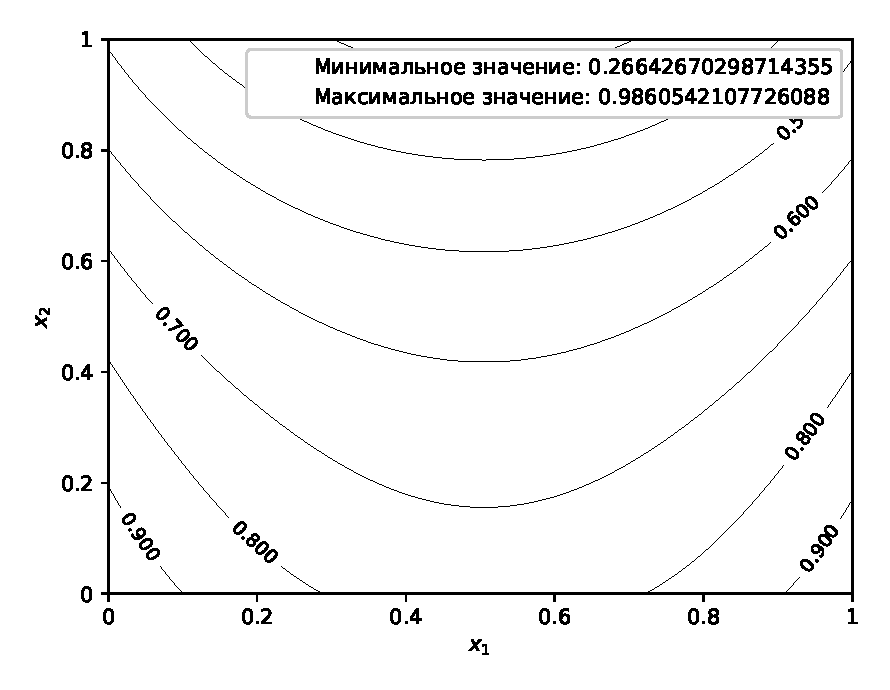
\includegraphics[width=1\linewidth]{jvm-2020/exp2/theta_auto}
        \\ а) Полученное решение $\theta$
    \end{minipage}
    \hfill
    \begin{minipage}[b][][b]{0.49\linewidth}
        \centering
        \includegraphics[width=1\linewidth]{jvm-2020/exp2/quality}
        \\ б) Изменение функционала качества
    \end{minipage}
    \caption{Результаты второго эксперимента}
    \label{fig:4_4:1}
\end{figure}

Представленные численные примеры иллюстрируют, что предложенный алгоритм успешно справляется
с нахождением численного решения задачи~\eqref{eq:2_2:eq1}--\eqref{eq:2_2:bc2}.


\textbf{Пример 3.}
Положим в условии~\eqref{eq:2_2:bc1}
$r=0.8 \cos (x)+0.1,\; u=\hat{u}=y$.
Далее рассчитываем состояние $\theta$ и $\varphi$ как решение
задачи~\eqref{eq:2_2:eq1}--\eqref{eq:2_2:bc2}
и в качестве $\theta_{b}$ выбираем граничные значения функции $\theta$ на Г.
Применяя предложенный алгоритм с начальным приближением $u_{0}=0.1$,
находим приближенное решение задачи $(C)$.
Квадрат разницы тестового и найденного решения представлен на рисунке~\ref{fig:4_4:2}а,
а также динамика функционала качества рисунке~\ref{fig:4_4:2}б.

\begin{figure}[ht]
    \begin{minipage}[b][][b]{0.49\linewidth}
        \centering
        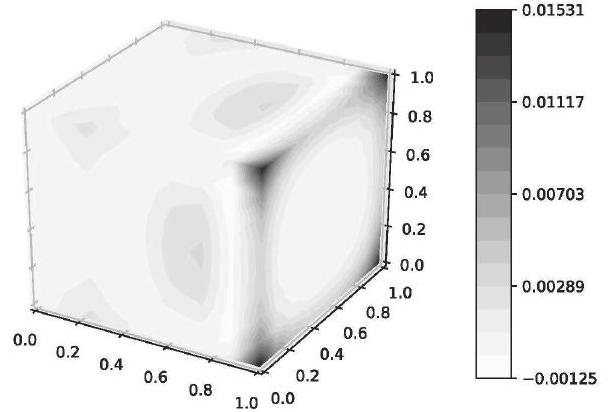
\includegraphics[width=1\linewidth]{jvm-2020/dvmg/1a}
        \\ а) $\left(\hat{u}-u_{100}\right)^{2}$
    \end{minipage}
    \hfill
    \begin{minipage}[b][][b]{0.49\linewidth}
        \centering
        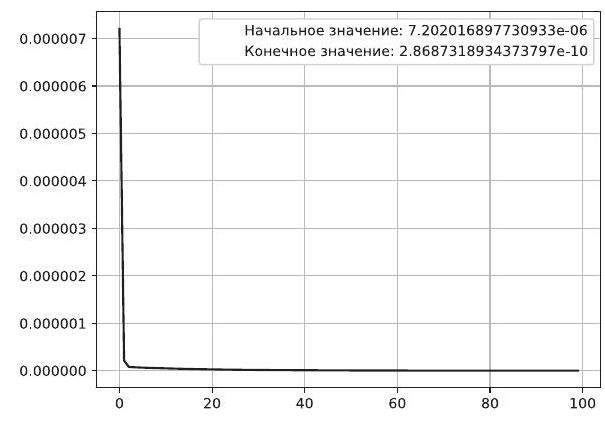
\includegraphics[width=1\linewidth]{jvm-2020/dvmg/1b}
        \\ б) Изменение функционала в зависимости от числа итераций
    \end{minipage}
    \caption{Результаты третьего эксперимента}
    \label{fig:4_4:2}
\end{figure}


\textbf{Пример 4.}
Зададим функции $\theta_{b}, q_{b}$ в краевом условии~\eqref{eq:2_2:bc2}
следующим образом:

\[
    \theta_{b}=0.1 z+0.3, \quad q_{b}=
    \begin{cases}
        0.11, & \text { если } z=1, \\
        0, & \text { если } 0<z<1, \\
        -0.15, & \text { если } z=0.
    \end{cases}
\]


В данном примере оптимальное управление $u$ в качестве тестового не задается.
На рисунках~\ref{fig:4_4:3}а,\ref{fig:4_4:3}б представлен результат работы алгоритма.

\begin{figure}[ht]
    \begin{minipage}[b][][b]{0.49\linewidth}
        \centering
        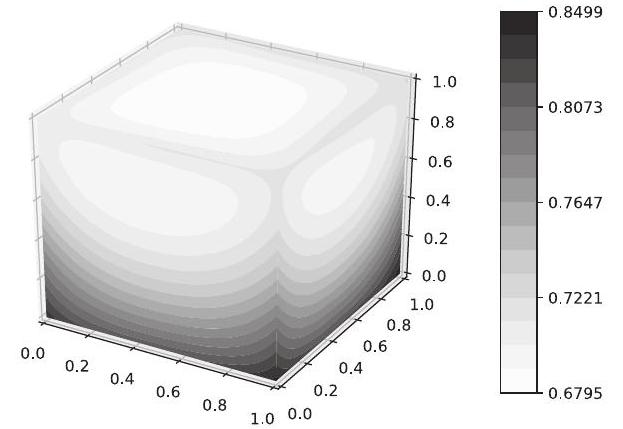
\includegraphics[width=0.9\linewidth]{jvm-2020/dvmg/2a}
        \\ а) Оптимальное управление
    \end{minipage}
    \hfill
    \begin{minipage}[b][][b]{0.49\linewidth}
        \centering
        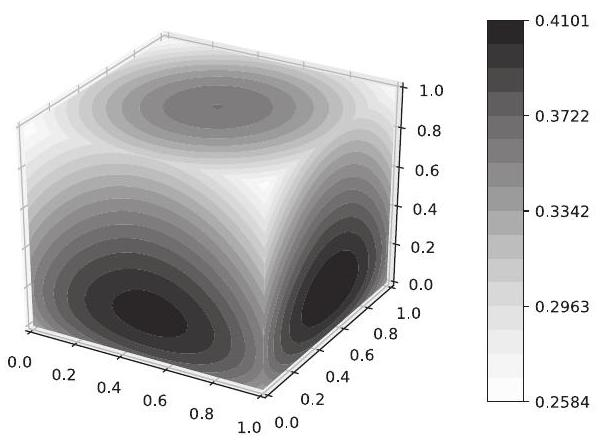
\includegraphics[width=1\linewidth]{jvm-2020/dvmg/2b}
        \\ б) Изменение функционала  %в зависимости от числа итераций
    \end{minipage}
    \caption{Результаты третьего эксперимента}
    \label{fig:4_4:3}
\end{figure}

Компоненты состояния, соответствующие найденному управлению, представлены на
рисунках~\ref{fig:4_4:4}а,\ref{fig:4_4:4}б.


\begin{figure}[ht]
    \begin{minipage}[b][][b]{0.49\linewidth}
        \centering
        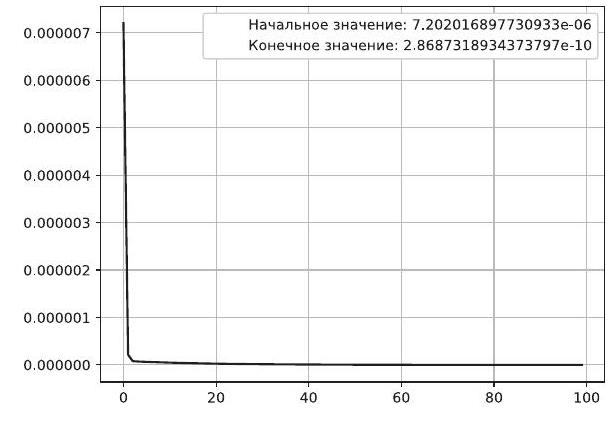
\includegraphics[width=1\linewidth]{jvm-2020/dvmg/3a}
        \\ а) Температура $\theta$
    \end{minipage}
    \hfill
    \begin{minipage}[b][][b]{0.49\linewidth}
        \centering
        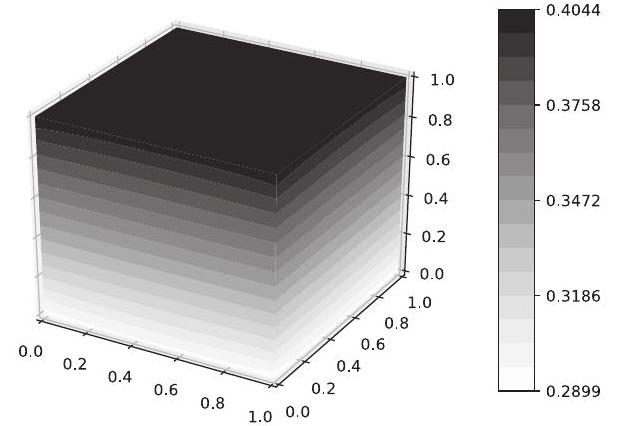
\includegraphics[width=1\linewidth]{jvm-2020/dvmg/3b}
        \\ б) Излучение $\varphi$
    \end{minipage}
    \caption{Результаты третьего эксперимента}
    \label{fig:4_4:4}
\end{figure}

\subsection{
    Задача сложного теплообмена с условиями
    Коши для температуры на части границы
}\label{subsec:ch4/sec4/subsec2}
    %jvm-mesenev-chebotarev

Представим итерационный алгоритм решения задачи оптимального управления.
Пусть $\tilde J_\lambda(u)=J_\lambda(\theta(u), u)$,
где $\theta(u)$ компонента решения
задачи~\eqref{eq:2_4:eq1},\eqref{eq:2_4:bc2},
соответствующая управлению $u\in U$.

В соответствии с~\eqref{eq:2_4:as} градиент функционала $\tilde J_\lambda(u)$ равен
\[ \tilde J'_\lambda (u) = \lambda u - p_2. \]
Здесь $p_2$ -- соответствующая компонента сопряженного состояния из системы ~\eqref{eq:2_4:as},
где $\hat{\theta}\coloneqq\theta(u)$.

%    \begin{algorithm}[H]
%        \caption{Алгоритм градиентного спуска}
%        \label{alg:algorithm}
%        \begin{algorithmic}[1]
%            \State Выбираем значение градиентного шага $\varepsilon$,
%            \State Выбираем количество итераций $N$,
%            \State Выбираем начальное приближение для управления $u_0 \in U$,
%            \For{$k \gets 0,1,2,\dots,N$}
%                \State Для данного $u_k$ рассчитываем состояние $y_k = \{\theta_k, \varphi_k\}$ --
%                решение задачи~\eqref{eq1},\eqref{bc1}.
%                \State Рассчитываем значение целевого функционала $J_\lambda(\theta_k, u_k)$.
%                \State Рассчитываем сопряженное состояние
%$p_k=\{p_{1k},p_{2k}\}$ из уравнений ~\eqref{OC1},
%                где $ \hat{\theta} \coloneqq \theta_k, \hat{u}=u_k$.
%                \State Пересчитываем управление $u_{k+1} = u_k - \varepsilon (\lambda u_k - p_2)$
%            \EndFor
%        \end{algorithmic}
%    \end{algorithm}
Значение параметра $\varepsilon$ выбирается эмпирически таким образом, чтобы значение
$\varepsilon (\lambda u_k - p_2)$ являлось существенной поправкой для $u_{k+1}$.
Количество итераций $N$ выбирается достаточным для выполнения условия
$J_\lambda(\theta_k, u_k) - J_\lambda(\theta_{k+1}, u_{k+1}) < \delta$, где $\delta > 0$
определяет точность расчетов.

Примеры, рассмотренные ниже, иллюстрируют работоспособность предложенного алгоритма при
малых, что важно, значениях параметра регуляризации $\lambda \leq 10^{-12}$.
В первом примере выполнены тестовые расчеты для куба.
Во втором примере рассмотрен куб с внутренней полостью.
Для численного решения прямой задачи с заданным управлением использовался
метод Ньютона для линеаризации задачи и ее решения методом конечных элементов.
Решение сопряженной системы, которая является линейной
при заданной температуре, не вызывает трудностей.
Для численного моделирования использовался солвер FEniCS~\cite{fenics},\cite{dolfin}.

Исходный код экспериментов можно найти по ссылке~\cite{mesenev-github}.

\textbf{Пример 1.}
Рассмотрим куб $\Omega = {(x, y, z), 0 \leq x,y,z \leq l}$ с границей
$\Gamma \equiv \Gamma_1 \cup \Gamma_2$, где
\[
    \Gamma_1 = \{(x, y, z), 0 \leq x,y, \leq l, z \in 0, l\}, \;
    \Gamma_2 = \partial \Omega \setminus \hat{\Gamma_1}.
\]
Будем считать, что
$l = 1~\text{см}$,
$a = 0.6[\text{см}^2/\text{c}]$,
$b = 0.025[\text{см}/\text{с}]$,
$\kappa_a = 1[\text{см}^{-1}]$,
$\alpha = 0.(3)[\text{см}]$.
Указанные параметры соответствуют стеклу~\cite{Grenkin2016a}.
Параметр регуляризации $\lambda=10^{-12}$.

Пусть граничные данные $q_b$ и $\theta_b$ в~\eqref{eq:2_4:bc1},\eqref{eq:2_4:bc2} имеют вид:
\begin{gather*}
    q_b = 0.5, \quad
    \theta_b = 0.1 + z/2
\end{gather*}
на все границе, а также начальное управление $u_0 = 0$.
Используя предложенный алгоритм решим задачу оптимального управления.

\begin{figure}[ht]
    \begin{minipage}[b][][b]{0.49\linewidth}
        \centering
        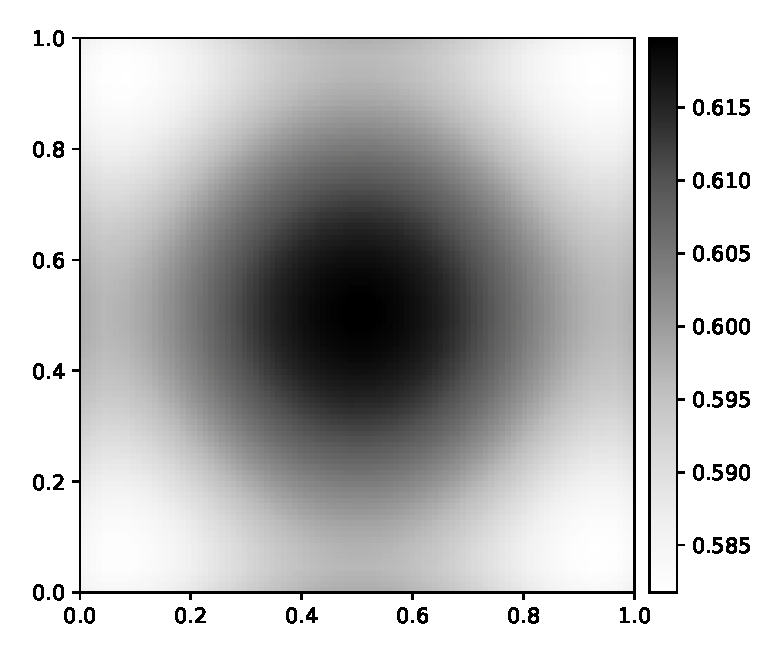
\includegraphics[width=1\linewidth]{jvm-2022/1_theta}
        \\ а) $\theta|_{z=1}$
    \end{minipage}
    \hfill
    \begin{minipage}[b][][b]{0.49\linewidth}
        \centering
        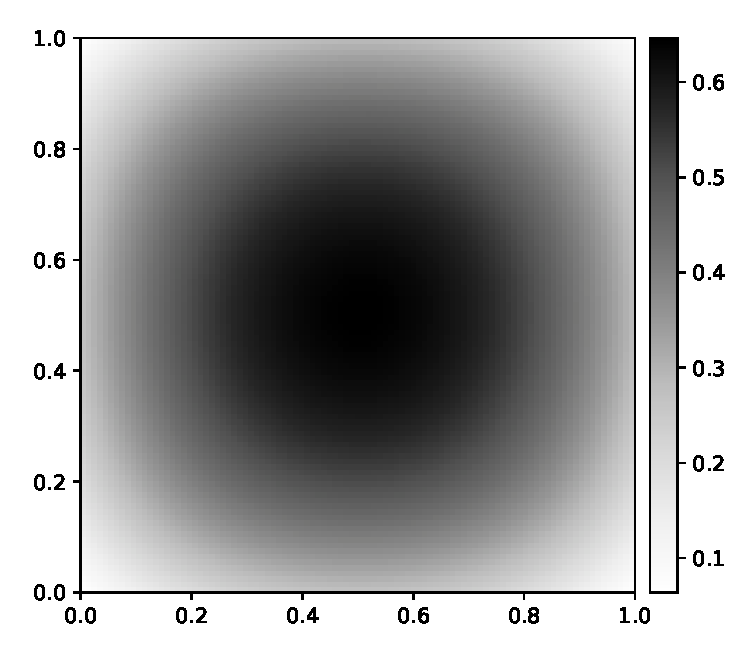
\includegraphics[width=1\linewidth]{jvm-2022/1_phi}
        \\ б) $\phi|_{z=1}$
    \end{minipage}
    \caption{Результаты первого эксперимента}
    \label{fig:4_4:5}
\end{figure}

На фиг.~\ref{fig:4_4:5}а,~\ref{fig:4_4:5}б представлены
полученные решения $\theta$ и $\phi$.
Начальное значение функционала качества равно $~0.025$ и
через сотню итераций становится равным $~5.e-05$.

\textbf{Пример 2.}
Рассмотрим двумерный случай: имеется квадрат
$S = \{(x, y), 0 \leq x,y,z \leq 1~\text{см.}\}$ с
круговой полостью $R$ с центром $b_0 =\{0.5, 0.5\}$
$R = \{r, \| r - b_0 \| \leq 0.15~\text{см.} \}$.
Рассматриваемая область $\Omega = S \setminus R$.
$\Gamma \equiv \partial \Omega = \partial C \cup \partial B$ при чём
\[
    \Gamma_2 = \partial R,
    \Gamma_1 = \partial S \setminus \Gamma_2.
\]
Параметры среды возьмём из примера 1.
Граничные данные $q_b$ и $\theta_b$ положим равными
\begin{gather*}
    \theta_b = 0.5, \\
    q_b =
    \begin{cases}
        0.2, & \text{если } x \in \Gamma_1 \\
        -0.2, & \text{если } x \in \Gamma_2.
    \end{cases}
\end{gather*}

\begin{figure}[ht]
    \begin{minipage}[b][][b]{0.49\linewidth}
        \centering
        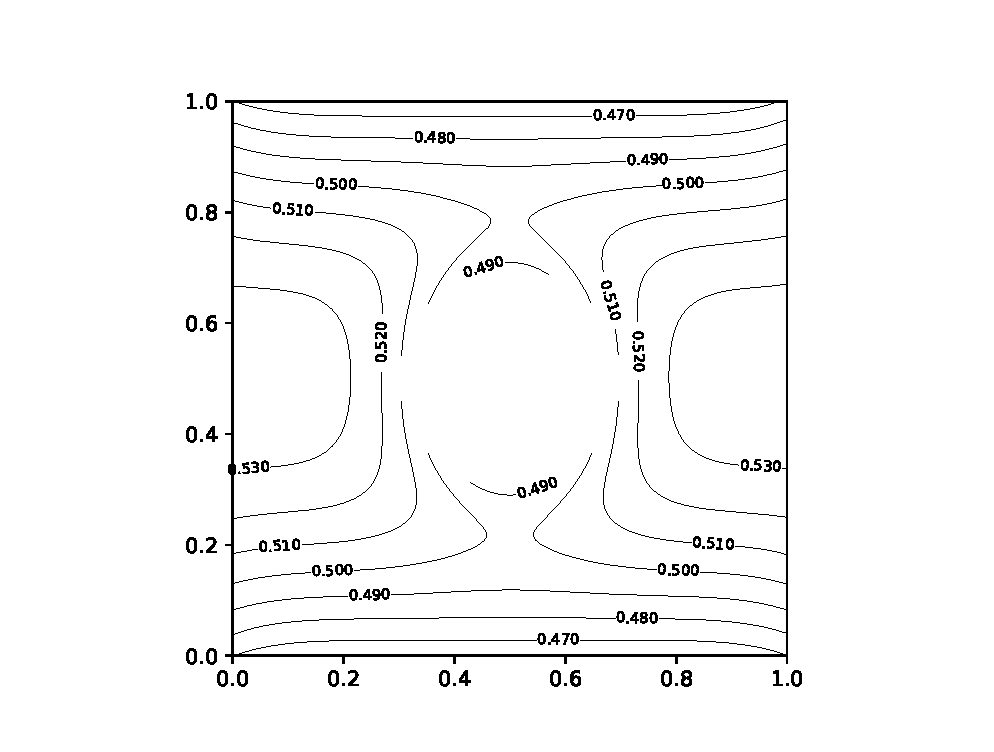
\includegraphics[width=1\linewidth]{jvm-2022/2_theta}
        \\ а) $\theta$
    \end{minipage}
    \hfill
    \begin{minipage}[b][][b]{0.49\linewidth}
        \centering
        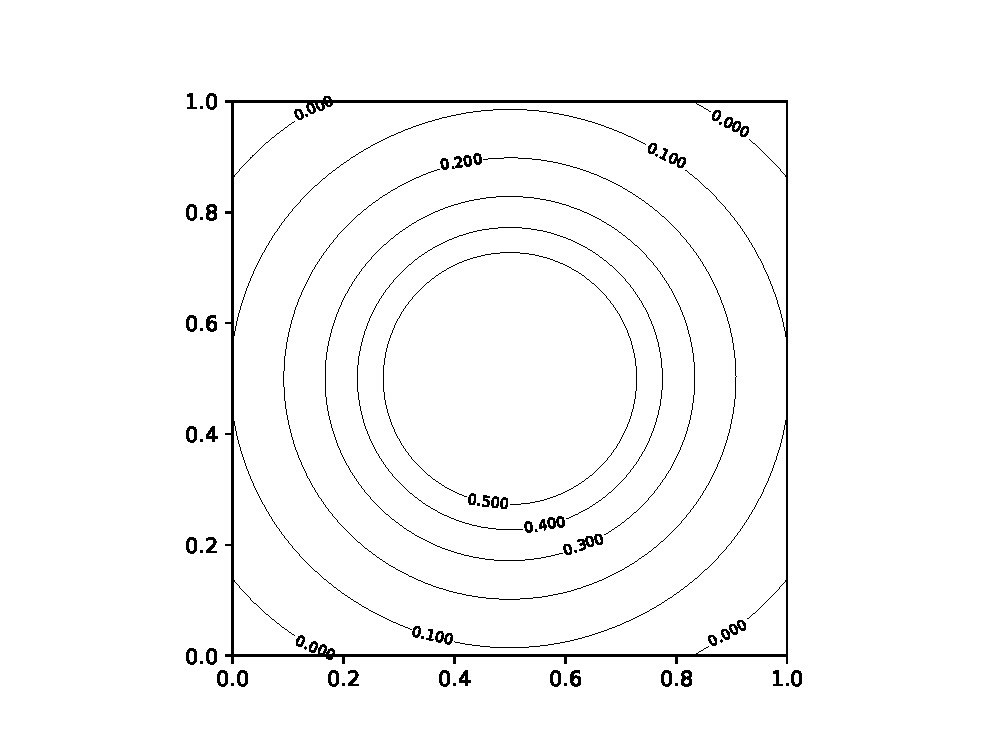
\includegraphics[width=1\linewidth]{jvm-2022/2_phi}
        \\ б) $\phi$
    \end{minipage}
    \caption{Результаты второго эксперимента}
    \label{fig:4_4:6}
\end{figure}
Начальное значение функционала качества $~0.045$.
После тридцати итераций $~6.2-05$.
Полученное состояние представлено рисунками ~\ref{fig:4_4:6}а,\ref{fig:4_4:6}б.


Представленные численные примеры демонстрируют,
что предложенный алгоритм успешно справляется
с нахождением численного решения задачи~\eqref{eq:2_4:eq1}--\eqref{eq:2_4:bc2}.



    \chapter*{Заключение}                       % Заголовок
\addcontentsline{toc}{chapter}{Заключение}  % Добавляем его в оглавление

%% Согласно ГОСТ Р 7.0.11-2011:
%% 5.3.3 В заключении диссертации излагают итоги выполненного исследования, рекомендации, перспективы дальнейшей разработки темы.
%% 9.2.3 В заключении автореферата диссертации излагают итоги данного исследования, рекомендации и перспективы дальнейшей разработки темы.
%% Поэтому имеет смысл сделать эту часть общей и загрузить из одного файла в автореферат и в диссертацию:

%% Согласно ГОСТ Р 7.0.11-2011:
%% 5.3.3 В заключении диссертации излагают итоги выполненного исследования, рекомендации, перспективы дальнейшей разработки темы.
%% 9.2.3 В заключении автореферата диссертации излагают итоги данного исследования, рекомендации и перспективы дальнейшей разработки темы.
В диссертации доказано существование квазирешения задачи нахождения
коэффициента отражения участка границы для стационарной модели,
по дополнительной информации о температурном поле.
Экспериментально поверена устойчивость получаемых
решений методом градиентного спуска.
Таким образом, получены важные с теоретической точки зрения результаты,
которые могут быть полезны при дальнейшем использовании
стационарных моделей сложного теплообмена и анализе обратных
задач в рамках нестационарных моделей сложного теплообмена.
Развитые методы исследования начально-краевых задач могут
применяться для изучения различных моделей, описываемых нелинейными
уравнениями со сходной структурой.

Разработанный комплекс программ для постановки численных экспериментов
показал свою надёжность и может в дальнейшем быть использован как
пример для решения подобных задач.

Разработан комплекс программ для проведения вычислительных экспериментов.
Для презентации результатов расчётов, помимо самих солверов,
был разработан программный комплекс для отрисовки
полученных расчётов в трёхмерных областях.

Исследование нестационарных моделей сложного теплообмена и соответствующих им
обратных задач является крайне перспективной областью математического моделирования
и в то же время достаточно сложной для теоретического
анализа и реализации численных решений.

В заключении автор выражает искреннюю благодарность научному руководителю
Чеботареву А.\ Ю.\ за его поддержку,
помощь, терпеливость и личный пример,
который сделал данную работу возможной.

Особую признательность автор хочет выразить Байдину А.\ В.,
Бризицкому Р.\ В., Артемьевой И.\ Л., чья поддержка оказалась
неоценимой в написании данной работы,
Кленину А.\ С., который стал источником мотивации в написании данного труда,
и Алексееву Г.\ В.\ за помощь в первых шагах научной деятельности автора.

Автор хотел бы отдельно поблагодарить Месенева В.\ П.\
за его неоценимый вклад в становление автора и бесконечную сопричастность к данной работе.
      % Заключение
%    \input{Dissertation/acronyms}        % Список сокращений и условных обозначений
%    \input{Dissertation/dictionary}      % Словарь терминов
    \input{Dissertation/references}      % Список литературы
    \clearpage
\ifdefmacro{\microtypesetup}{\microtypesetup{protrusion=false}}{} % не рекомендуется применять пакет микротипографики к автоматически генерируемым спискам
\listoffigures  % Список изображений

%%% Список таблиц %%%
% (ГОСТ Р 7.0.11-2011, 5.3.10)
%\clearpage
%\listoftables   % Список таблиц
\ifdefmacro{\microtypesetup}{\microtypesetup{protrusion=true}}{}
\newpage
           % Списки таблиц и изображений (иллюстративный материал)

    \setcounter{totalchapter}{\value{chapter}} % Подсчёт количества глав

%%% Настройки для приложений
    \appendix
% Оформление заголовков приложений ближе к ГОСТ:
    \setlength{\midchapskip}{20pt}
    \renewcommand*{\afterchapternum}{\par\nobreak\vskip \midchapskip}
    \renewcommand\thechapter{\Asbuk{chapter}} % Чтобы приложения русскими буквами нумеровались

    \chapter{Приложения}
\label{ch:ch5}

\lstinputlisting[lastline=78,language=Python,
    caption={Решение краевой задачи с использованием солвера FEniCS},label={lst:boundary}]{listings/boundary.py}

%\lstinputlisting[lastline=78,language=Python,
%caption={Моделирование квазилинейной задачи при различных функциях $k(\theta)$},
%label={lst:theta_gap}]{listings/theta_gap.py}
        % Приложения

    \setcounter{totalappendix}{\value{chapter}} % Подсчёт количества приложений

\end{document}
